\documentclass[10pt]{report}
\usepackage{lmodern}
\usepackage{graphicx}
\usepackage{varwidth}
\usepackage{enumitem}
\usepackage{amsmath}
\usepackage{amssymb}
\usepackage{mathtools}
\usepackage{pifont}
\usepackage{arydshln}
\usepackage{tikz}
\usepackage{lscape}
\usepackage{bm}
\usepackage{nicefrac}
\usepackage{physics}
\usepackage{fontsize}
\usepackage[landscape]{geometry}
\geometry{a4paper, total={296mm,210mm}, left=-5mm, top=0mm}
\renewcommand{\labelenumi}{\bfseries(\alph{enumi})\phantom{x}}
\newcommand\omicron{o}
\hfuzz=50pt
\setlist[enumerate]{leftmargin=0pt,itemindent=34pt}
\pagenumbering{gobble}
\setlength{\tabcolsep}{0pt}
\begin{document}
\thispagestyle{empty}
\begin{tabular}{c:c}
\begin{minipage}[c][104.5mm][t]{0.5\linewidth}
\begin{center}
\vspace{7mm}
{\huge Volné extrémy, skupina \textit{Alpha $\alpha$} -\romannumeral1}\\[5mm]
\textit{Jméno:}\phantom{xxxxxxxxxxxxxxxxxxxxxxxxxxxxxxxxxxxxxxxxxxxxxxxxxxxxxxxxxxxxxxxxx}\\[5mm]
\begin{minipage}{0.95\linewidth}
\begin{center}
Cílem je najít \textbf{volné extrémy} funkce $f(x,y)$ zadané v \textbf{(a)}.\\Postupuj podle krokú v \textbf{(b)} až \textbf{(f)}. Pokud se medzivýsledky shodujú s těmi za otazníky,\\tak napravo obarvi příslušející kroužek načerno. \textbf{Spolu odevzdejte výsledné slovo}.
\end{center}
\end{minipage}
\\[1mm]
\begin{minipage}{0.79\linewidth}
\begin{center}
\begin{varwidth}{\linewidth}
\begin{enumerate}
\normalsize
\item $f(x,y)=x^3-6x^2-15x-1+24y+3y^2-y^3$\quad \dotfill\; ???\;\dotfill \quad vybarvi
\item Najdi parciální derivaci podle $x$, $\pdv{f}{x}=$\quad \dotfill\; ???\;\dotfill \quad $3x^2-12x-15$
\item Najdi stacionární body v $x$\quad \dotfill\; ???\;\dotfill \quad $x_1+x_2=4$
\item Najdi parciální derivaci podle $y$, $\pdv{f}{y}=$\quad \dotfill\; ???\;\dotfill \quad $-3y^2+6y+24$
\item Najdi stacionární body v $y$\quad \dotfill\; ???\;\dotfill \quad $y_1+y_2=2$
\item Najdi funkční hodnoty vo všech stacionárních bodech \\ \phantom{xxxxxx} a vyber tu najvětší. $f_{\text{max}}(x,y)=$\quad \dotfill\; ???\;\dotfill \quad $-21$
\end{enumerate}
\end{varwidth}
\end{center}
\end{minipage}
\begin{minipage}{0.20\linewidth}
\begin{center}
{\Huge\bfseries 1.} \\[2mm]
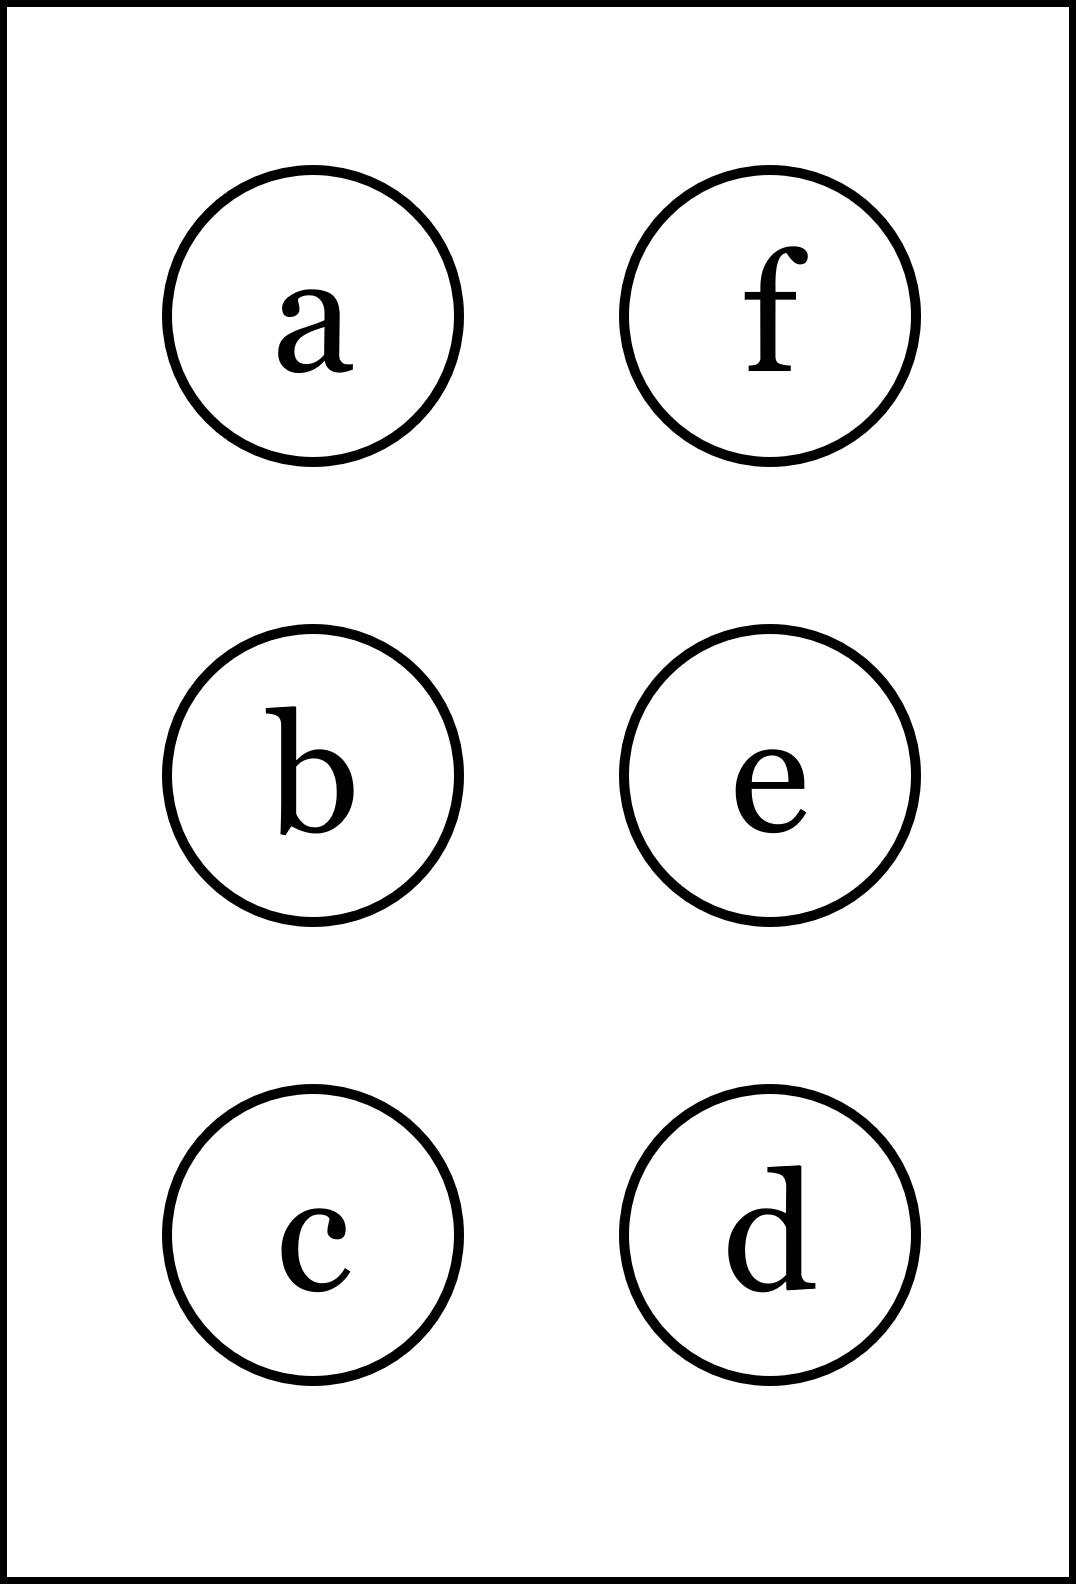
\includegraphics[height=40mm]{../images/braille.png}
{\small Písmeno Braillovej abecedy}
\end{center}
\end{minipage}
\end{center}
\end{minipage}
&
\begin{minipage}[c][104.5mm][t]{0.5\linewidth}
\begin{center}
\vspace{7mm}
{\huge Volné extrémy, skupina \textit{Alpha $\alpha$} -\romannumeral2}\\[5mm]
\textit{Jméno:}\phantom{xxxxxxxxxxxxxxxxxxxxxxxxxxxxxxxxxxxxxxxxxxxxxxxxxxxxxxxxxxxxxxxxx}\\[5mm]
\begin{minipage}{0.95\linewidth}
\begin{center}
Cílem je najít \textbf{volné extrémy} funkce $f(x,y)$ zadané v \textbf{(a)}.\\Postupuj podle krokú v \textbf{(b)} až \textbf{(f)}. Pokud se medzivýsledky shodujú s těmi za otazníky,\\tak napravo obarvi příslušející kroužek načerno. \textbf{Spolu odevzdejte výsledné slovo}.
\end{center}
\end{minipage}
\\[1mm]
\begin{minipage}{0.79\linewidth}
\begin{center}
\begin{varwidth}{\linewidth}
\begin{enumerate}
\normalsize
\item $f(x,y)=-x^3-9x^2+21x-2-45y+3y^2+y^3$\quad \dotfill\; ???\;\dotfill \quad vybarvi
\item Najdi parciální derivaci podle $x$, $\pdv{f}{x}=$\quad \dotfill\; ???\;\dotfill \quad $-3x^2-9x+21$
\item Najdi stacionární body v $x$\quad \dotfill\; ???\;\dotfill \quad $x_1+x_2=-6$
\item Najdi parciální derivaci podle $y$, $\pdv{f}{y}=$\quad \dotfill\; ???\;\dotfill \quad $3y^2+6y-36$
\item Najdi stacionární body v $y$\quad \dotfill\; ???\;\dotfill \quad $y_1+y_2=-2$
\item Najdi funkční hodnoty vo všech stacionárních bodech \\ \phantom{xxxxxx} a vyber tu najvětší. $f_{\text{max}}(x,y)=$\quad \dotfill\; ???\;\dotfill \quad $-72$
\end{enumerate}
\end{varwidth}
\end{center}
\end{minipage}
\begin{minipage}{0.20\linewidth}
\begin{center}
{\Huge\bfseries 2.} \\[2mm]
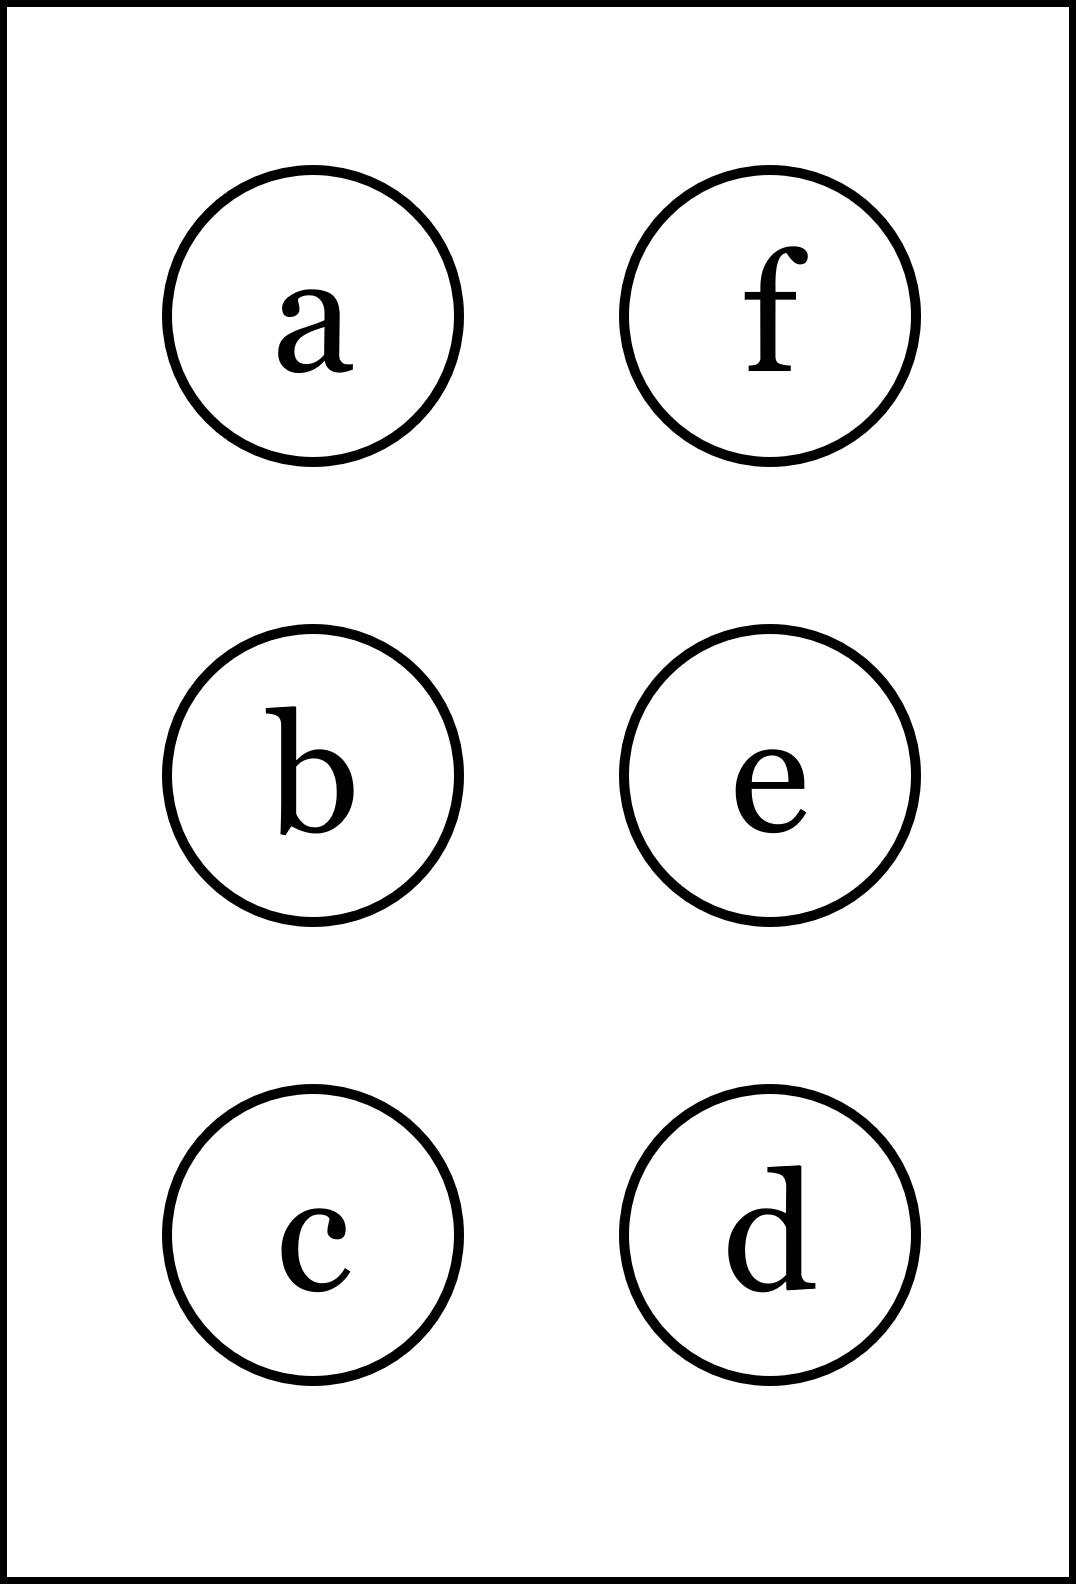
\includegraphics[height=40mm]{../images/braille.png}
{\small Písmeno Braillovej abecedy}
\end{center}
\end{minipage}
\end{center}
\end{minipage}
\\ \hdashline
\begin{minipage}[c][104.5mm][t]{0.5\linewidth}
\begin{center}
\vspace{7mm}
{\huge Volné extrémy, skupina \textit{Alpha $\alpha$} -\romannumeral3}\\[5mm]
\textit{Jméno:}\phantom{xxxxxxxxxxxxxxxxxxxxxxxxxxxxxxxxxxxxxxxxxxxxxxxxxxxxxxxxxxxxxxxxx}\\[5mm]
\begin{minipage}{0.95\linewidth}
\begin{center}
Cílem je najít \textbf{volné extrémy} funkce $f(x,y)$ zadané v \textbf{(a)}.\\Postupuj podle krokú v \textbf{(b)} až \textbf{(f)}. Pokud se medzivýsledky shodujú s těmi za otazníky,\\tak napravo obarvi příslušející kroužek načerno. \textbf{Spolu odevzdejte výsledné slovo}.
\end{center}
\end{minipage}
\\[1mm]
\begin{minipage}{0.79\linewidth}
\begin{center}
\begin{varwidth}{\linewidth}
\begin{enumerate}
\normalsize
\item $f(x,y)=x^3+6x^2+9x-1+21y+9y^2-y^3$\quad \dotfill\; ???\;\dotfill \quad vybarvi
\item Najdi parciální derivaci podle $x$, $\pdv{f}{x}=$\quad \dotfill\; ???\;\dotfill \quad $3x^2+12x+9$
\item Najdi stacionární body v $x$\quad \dotfill\; ???\;\dotfill \quad $x_1+x_2=-4$
\item Najdi parciální derivaci podle $y$, $\pdv{f}{y}=$\quad \dotfill\; ???\;\dotfill \quad $-3y^2+18y+12$
\item Najdi stacionární body v $y$\quad \dotfill\; ???\;\dotfill \quad $y_1+y_2=6$
\item Najdi funkční hodnoty vo všech stacionárních bodech \\ \phantom{xxxxxx} a vyber tu najvětší. $f_{\text{max}}(x,y)=$\quad \dotfill\; ???\;\dotfill \quad $-12$
\end{enumerate}
\end{varwidth}
\end{center}
\end{minipage}
\begin{minipage}{0.20\linewidth}
\begin{center}
{\Huge\bfseries 3.} \\[2mm]
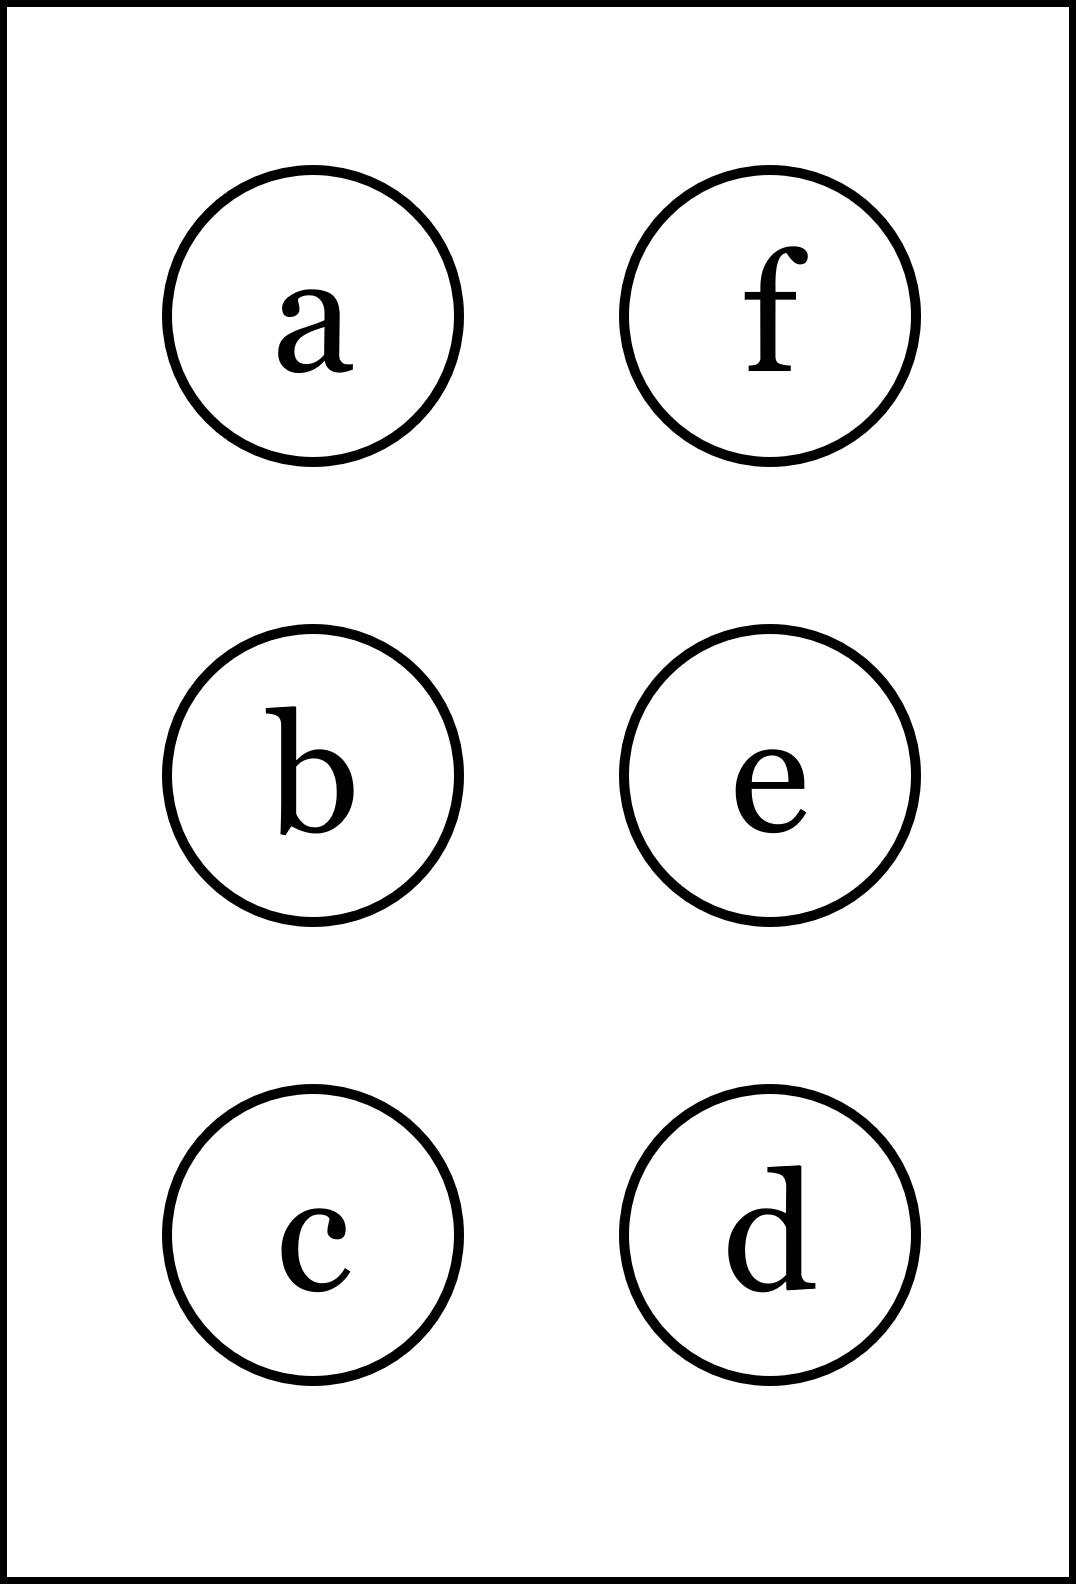
\includegraphics[height=40mm]{../images/braille.png}
{\small Písmeno Braillovej abecedy}
\end{center}
\end{minipage}
\end{center}
\end{minipage}
&
\begin{minipage}[c][104.5mm][t]{0.5\linewidth}
\begin{center}
\vspace{7mm}
{\huge Volné extrémy, skupina \textit{Alpha $\alpha$} -\romannumeral4}\\[5mm]
\textit{Jméno:}\phantom{xxxxxxxxxxxxxxxxxxxxxxxxxxxxxxxxxxxxxxxxxxxxxxxxxxxxxxxxxxxxxxxxx}\\[5mm]
\begin{minipage}{0.95\linewidth}
\begin{center}
Cílem je najít \textbf{volné extrémy} funkce $f(x,y)$ zadané v \textbf{(a)}.\\Postupuj podle krokú v \textbf{(b)} až \textbf{(f)}. Pokud se medzivýsledky shodujú s těmi za otazníky,\\tak napravo obarvi příslušející kroužek načerno. \textbf{Spolu odevzdejte výsledné slovo}.
\end{center}
\end{minipage}
\\[1mm]
\begin{minipage}{0.79\linewidth}
\begin{center}
\begin{varwidth}{\linewidth}
\begin{enumerate}
\normalsize
\item $f(x,y)=-4x^3-12x^2+36x+3-96y-12y^2+4y^3$\quad \dotfill\; ???\;\dotfill \quad vybarvi
\item Najdi parciální derivaci podle $x$, $\pdv{f}{x}=$\quad \dotfill\; ???\;\dotfill \quad $-12x^2-12x+36$
\item Najdi stacionární body v $x$\quad \dotfill\; ???\;\dotfill \quad $x_1+x_2=-1$
\item Najdi parciální derivaci podle $y$, $\pdv{f}{y}=$\quad \dotfill\; ???\;\dotfill \quad $12y^2-24y-72$
\item Najdi stacionární body v $y$\quad \dotfill\; ???\;\dotfill \quad $y_1+y_2=2$
\item Najdi funkční hodnoty vo všech stacionárních bodech \\ \phantom{xxxxxx} a vyber tu najvětší. $f_{\text{max}}(x,y)=$\quad \dotfill\; ???\;\dotfill \quad $135$
\end{enumerate}
\end{varwidth}
\end{center}
\end{minipage}
\begin{minipage}{0.20\linewidth}
\begin{center}
{\Huge\bfseries 4.} \\[2mm]
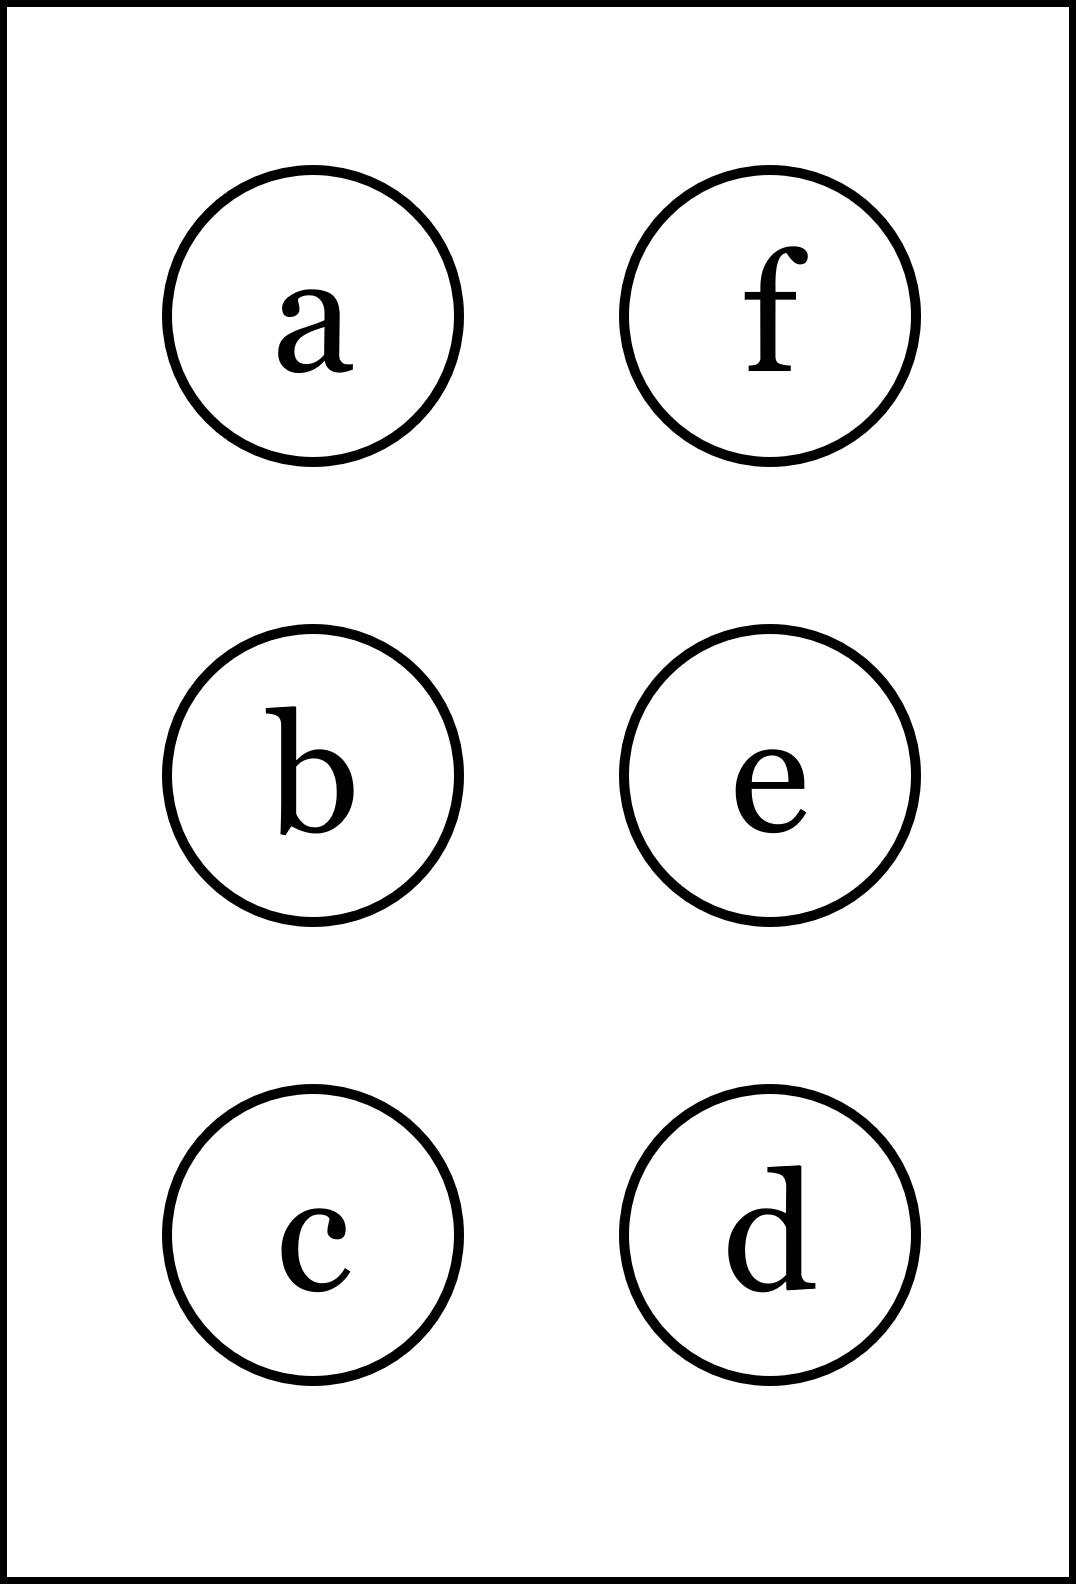
\includegraphics[height=40mm]{../images/braille.png}
{\small Písmeno Braillovej abecedy}
\end{center}
\end{minipage}
\end{center}
\end{minipage}
%
\end{tabular}
\newpage
\thispagestyle{empty}
\begin{tabular}{c:c}
\begin{minipage}[c][104.5mm][t]{0.5\linewidth}
\begin{center}
\vspace{7mm}
{\huge Volné extrémy, skupina \textit{Beta $\beta$} -\romannumeral1}\\[5mm]
\textit{Jméno:}\phantom{xxxxxxxxxxxxxxxxxxxxxxxxxxxxxxxxxxxxxxxxxxxxxxxxxxxxxxxxxxxxxxxxx}\\[5mm]
\begin{minipage}{0.95\linewidth}
\begin{center}
Cílem je najít \textbf{volné extrémy} funkce $f(x,y)$ zadané v \textbf{(a)}.\\Postupuj podle krokú v \textbf{(b)} až \textbf{(f)}. Pokud se medzivýsledky shodujú s těmi za otazníky,\\tak napravo obarvi příslušející kroužek načerno. \textbf{Spolu odevzdejte výsledné slovo}.
\end{center}
\end{minipage}
\\[1mm]
\begin{minipage}{0.79\linewidth}
\begin{center}
\begin{varwidth}{\linewidth}
\begin{enumerate}
\normalsize
\item $f(x,y)=-6x^3-18x^2+144x-3+45y-30y^2+5y^3$\quad \dotfill\; ???\;\dotfill \quad vybarvi
\item Najdi parciální derivaci podle $x$, $\pdv{f}{x}=$\quad \dotfill\; ???\;\dotfill \quad $-18x^2-18x+144$
\item Najdi stacionární body v $x$\quad \dotfill\; ???\;\dotfill \quad $x_1+x_2=-1$
\item Najdi parciální derivaci podle $y$, $\pdv{f}{y}=$\quad \dotfill\; ???\;\dotfill \quad $15y^2-60y+15$
\item Najdi stacionární body v $y$\quad \dotfill\; ???\;\dotfill \quad $y_1+y_2=4$
\item Najdi funkční hodnoty vo všech stacionárních bodech \\ \phantom{xxxxxx} a vyber tu najvětší. $f_{\text{max}}(x,y)=$\quad \dotfill\; ???\;\dotfill \quad $-483$
\end{enumerate}
\end{varwidth}
\end{center}
\end{minipage}
\begin{minipage}{0.20\linewidth}
\begin{center}
{\Huge\bfseries 1.} \\[2mm]
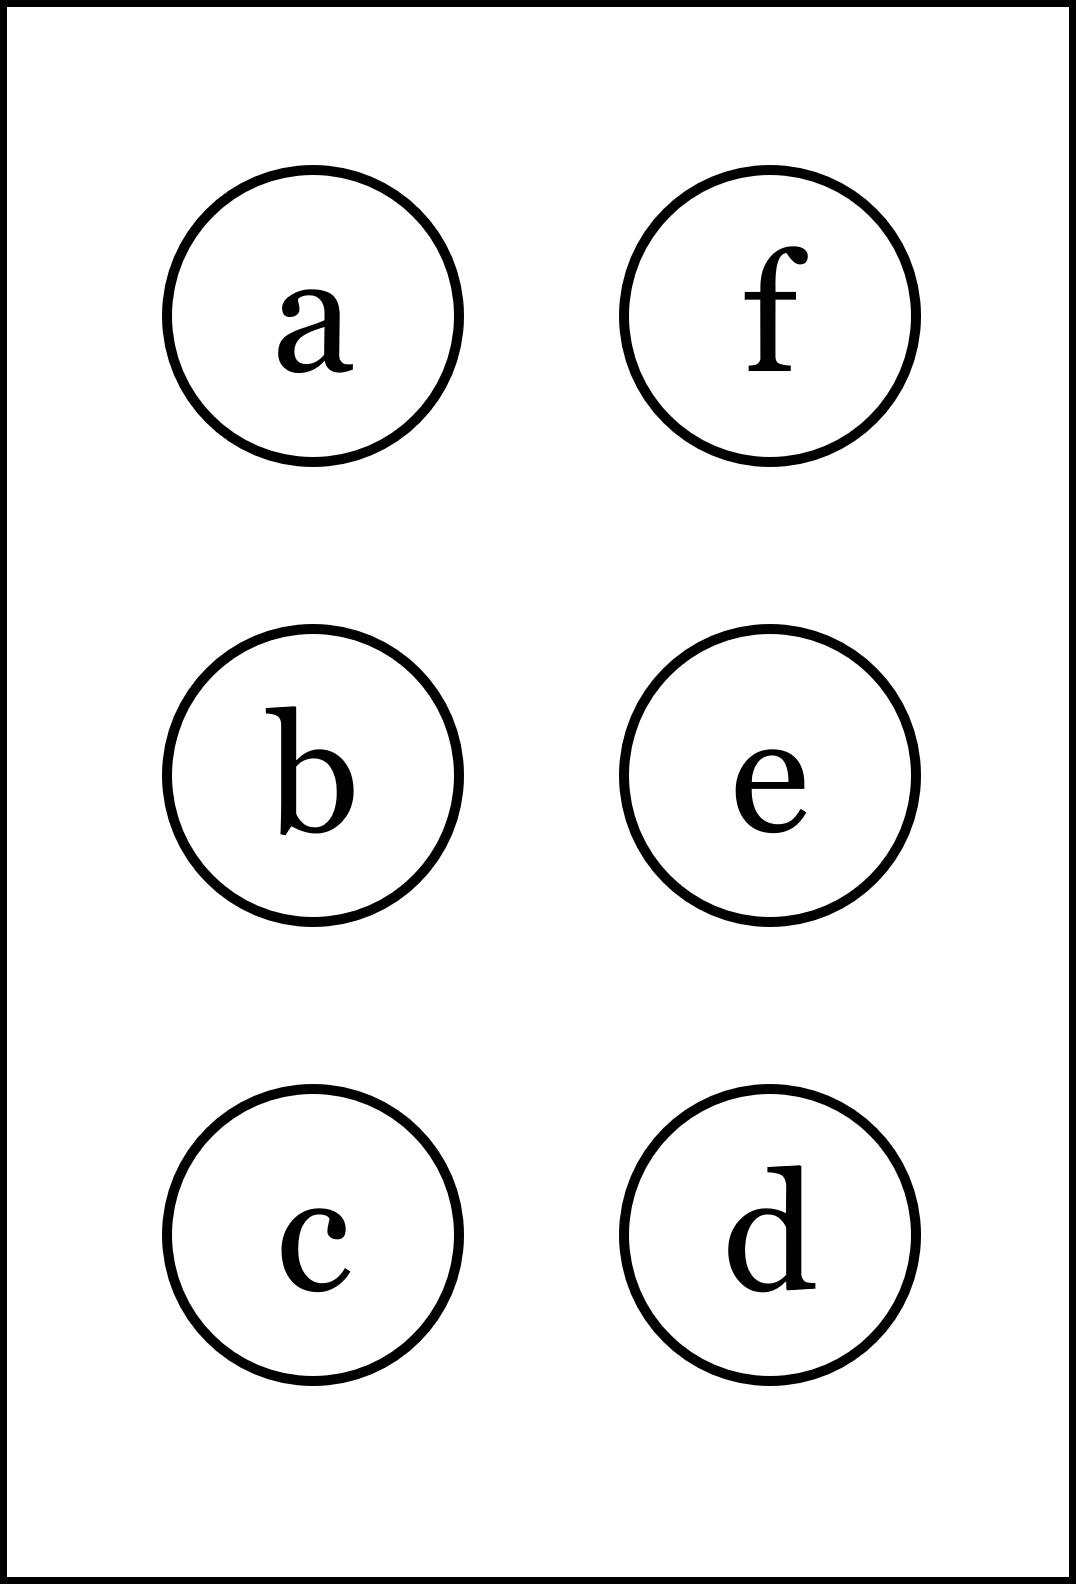
\includegraphics[height=40mm]{../images/braille.png}
{\small Písmeno Braillovej abecedy}
\end{center}
\end{minipage}
\end{center}
\end{minipage}
&
\begin{minipage}[c][104.5mm][t]{0.5\linewidth}
\begin{center}
\vspace{7mm}
{\huge Volné extrémy, skupina \textit{Beta $\beta$} -\romannumeral2}\\[5mm]
\textit{Jméno:}\phantom{xxxxxxxxxxxxxxxxxxxxxxxxxxxxxxxxxxxxxxxxxxxxxxxxxxxxxxxxxxxxxxxxx}\\[5mm]
\begin{minipage}{0.95\linewidth}
\begin{center}
Cílem je najít \textbf{volné extrémy} funkce $f(x,y)$ zadané v \textbf{(a)}.\\Postupuj podle krokú v \textbf{(b)} až \textbf{(f)}. Pokud se medzivýsledky shodujú s těmi za otazníky,\\tak napravo obarvi příslušející kroužek načerno. \textbf{Spolu odevzdejte výsledné slovo}.
\end{center}
\end{minipage}
\\[1mm]
\begin{minipage}{0.79\linewidth}
\begin{center}
\begin{varwidth}{\linewidth}
\begin{enumerate}
\normalsize
\item $f(x,y)=x^3-3x^2-24x-1+36y+12y^2-4y^3$\quad \dotfill\; ???\;\dotfill \quad vybarvi
\item Najdi parciální derivaci podle $x$, $\pdv{f}{x}=$\quad \dotfill\; ???\;\dotfill \quad $3x^2-6x-24$
\item Najdi stacionární body v $x$\quad \dotfill\; ???\;\dotfill \quad $x_1+x_2=2$
\item Najdi parciální derivaci podle $y$, $\pdv{f}{y}=$\quad \dotfill\; ???\;\dotfill \quad $-12y^2+24y+24$
\item Najdi stacionární body v $y$\quad \dotfill\; ???\;\dotfill \quad $y_1+y_2=2$
\item Najdi funkční hodnoty vo všech stacionárních bodech \\ \phantom{xxxxxx} a vyber tu najvětší. $f_{\text{max}}(x,y)=$\quad \dotfill\; ???\;\dotfill \quad $7$
\end{enumerate}
\end{varwidth}
\end{center}
\end{minipage}
\begin{minipage}{0.20\linewidth}
\begin{center}
{\Huge\bfseries 2.} \\[2mm]
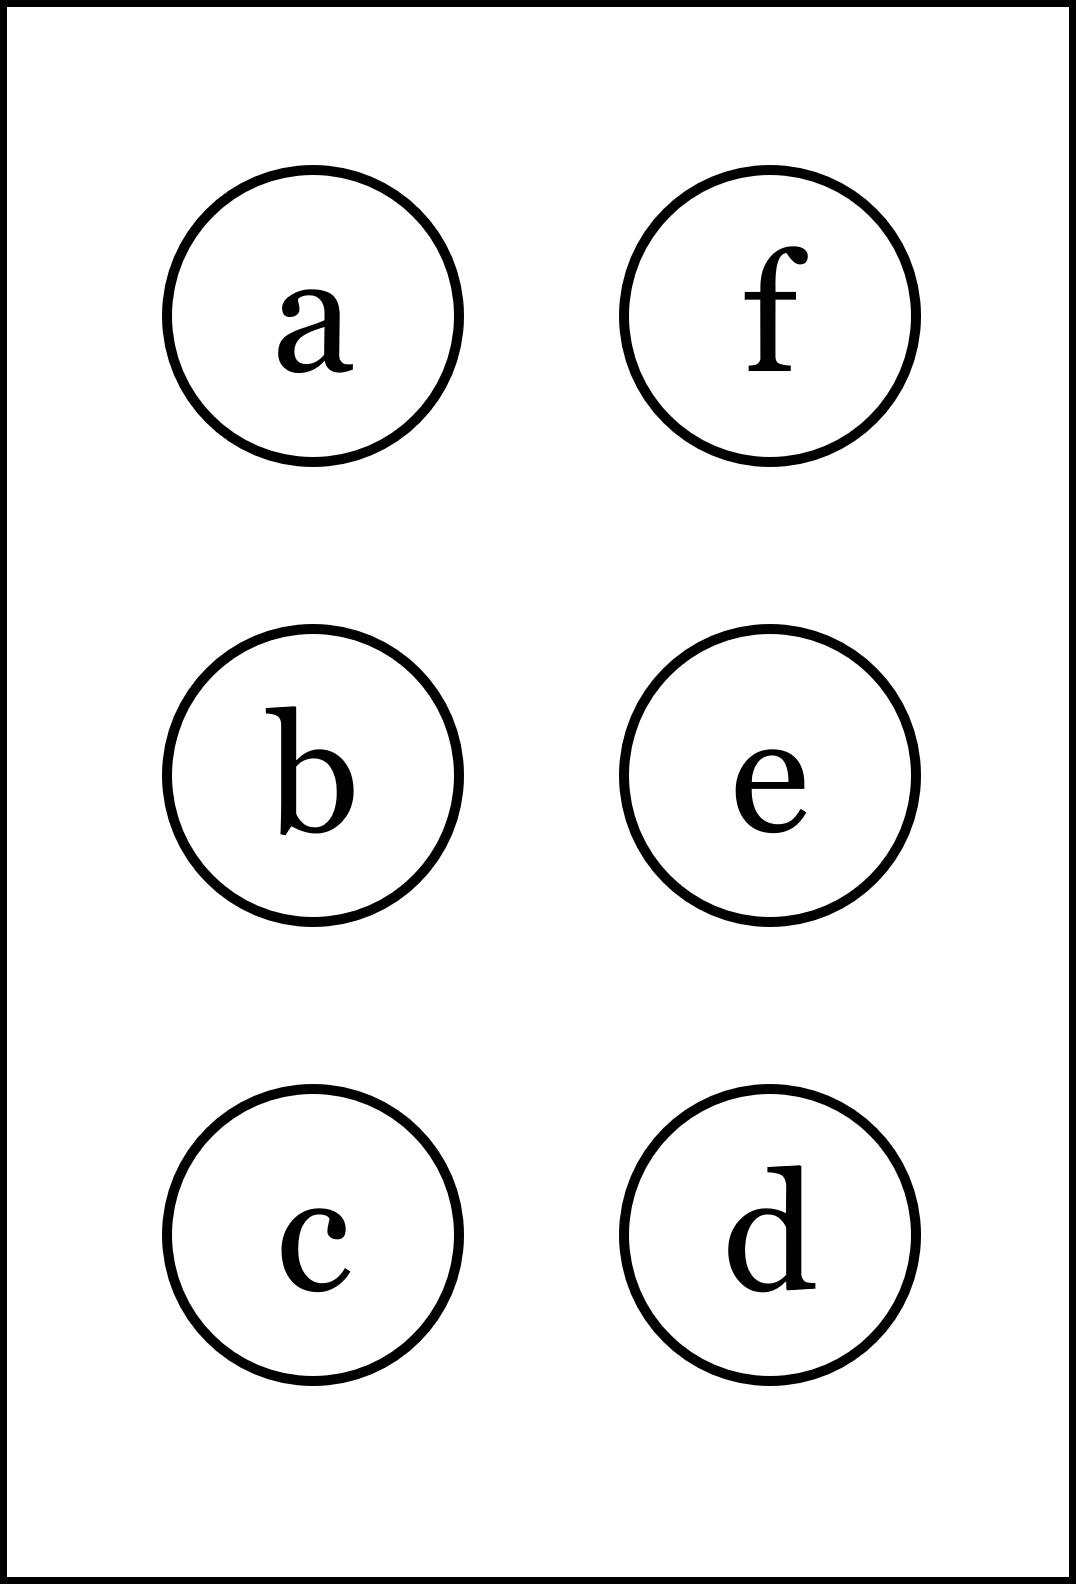
\includegraphics[height=40mm]{../images/braille.png}
{\small Písmeno Braillovej abecedy}
\end{center}
\end{minipage}
\end{center}
\end{minipage}
\\ \hdashline
\begin{minipage}[c][104.5mm][t]{0.5\linewidth}
\begin{center}
\vspace{7mm}
{\huge Volné extrémy, skupina \textit{Beta $\beta$} -\romannumeral3}\\[5mm]
\textit{Jméno:}\phantom{xxxxxxxxxxxxxxxxxxxxxxxxxxxxxxxxxxxxxxxxxxxxxxxxxxxxxxxxxxxxxxxxx}\\[5mm]
\begin{minipage}{0.95\linewidth}
\begin{center}
Cílem je najít \textbf{volné extrémy} funkce $f(x,y)$ zadané v \textbf{(a)}.\\Postupuj podle krokú v \textbf{(b)} až \textbf{(f)}. Pokud se medzivýsledky shodujú s těmi za otazníky,\\tak napravo obarvi příslušející kroužek načerno. \textbf{Spolu odevzdejte výsledné slovo}.
\end{center}
\end{minipage}
\\[1mm]
\begin{minipage}{0.79\linewidth}
\begin{center}
\begin{varwidth}{\linewidth}
\begin{enumerate}
\normalsize
\item $f(x,y)=-x^3-9x^2+81x-7+48y+6y^2-2y^3$\quad \dotfill\; ???\;\dotfill \quad nebarvi
\item Najdi parciální derivaci podle $x$, $\pdv{f}{x}=$\quad \dotfill\; ???\;\dotfill \quad $-3x^2-18x+81$
\item Najdi stacionární body v $x$\quad \dotfill\; ???\;\dotfill \quad $x_1+x_2=-5$
\item Najdi parciální derivaci podle $y$, $\pdv{f}{y}=$\quad \dotfill\; ???\;\dotfill \quad $-6y^2+12y+36$
\item Najdi stacionární body v $y$\quad \dotfill\; ???\;\dotfill \quad $y_1+y_2=3$
\item Najdi funkční hodnoty vo všech stacionárních bodech \\ \phantom{xxxxxx} a vyber tu najvětší. $f_{\text{max}}(x,y)=$\quad \dotfill\; ???\;\dotfill \quad $288$
\end{enumerate}
\end{varwidth}
\end{center}
\end{minipage}
\begin{minipage}{0.20\linewidth}
\begin{center}
{\Huge\bfseries 3.} \\[2mm]
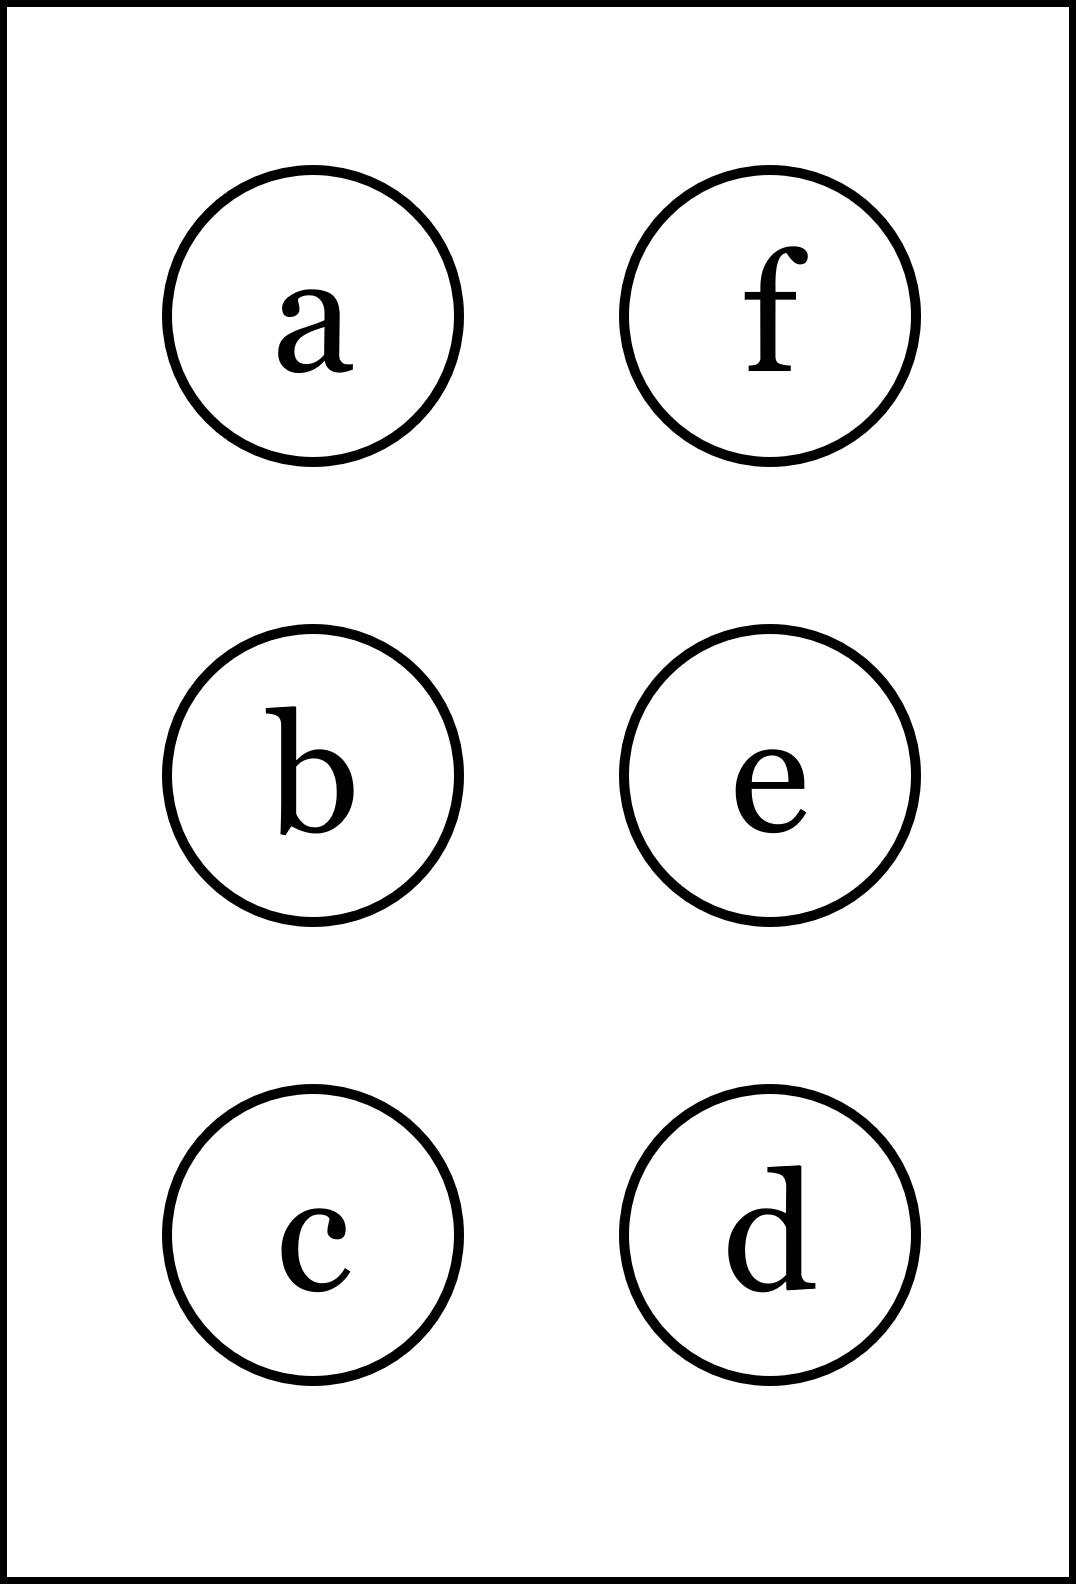
\includegraphics[height=40mm]{../images/braille.png}
{\small Písmeno Braillovej abecedy}
\end{center}
\end{minipage}
\end{center}
\end{minipage}
&
\begin{minipage}[c][104.5mm][t]{0.5\linewidth}
\begin{center}
\vspace{7mm}
{\huge Volné extrémy, skupina \textit{Beta $\beta$} -\romannumeral4}\\[5mm]
\textit{Jméno:}\phantom{xxxxxxxxxxxxxxxxxxxxxxxxxxxxxxxxxxxxxxxxxxxxxxxxxxxxxxxxxxxxxxxxx}\\[5mm]
\begin{minipage}{0.95\linewidth}
\begin{center}
Cílem je najít \textbf{volné extrémy} funkce $f(x,y)$ zadané v \textbf{(a)}.\\Postupuj podle krokú v \textbf{(b)} až \textbf{(f)}. Pokud se medzivýsledky shodujú s těmi za otazníky,\\tak napravo obarvi příslušející kroužek načerno. \textbf{Spolu odevzdejte výsledné slovo}.
\end{center}
\end{minipage}
\\[1mm]
\begin{minipage}{0.79\linewidth}
\begin{center}
\begin{varwidth}{\linewidth}
\begin{enumerate}
\normalsize
\item $f(x,y)=-6x^3+36x^2+90x+2+75y+30y^2-5y^3$\quad \dotfill\; ???\;\dotfill \quad vybarvi
\item Najdi parciální derivaci podle $x$, $\pdv{f}{x}=$\quad \dotfill\; ???\;\dotfill \quad $-18x^2+36x+90$
\item Najdi stacionární body v $x$\quad \dotfill\; ???\;\dotfill \quad $x_1+x_2=4$
\item Najdi parciální derivaci podle $y$, $\pdv{f}{y}=$\quad \dotfill\; ???\;\dotfill \quad $-15y^2+60y+45$
\item Najdi stacionární body v $y$\quad \dotfill\; ???\;\dotfill \quad $y_1+y_2=5$
\item Najdi funkční hodnoty vo všech stacionárních bodech \\ \phantom{xxxxxx} a vyber tu najvětší. $f_{\text{max}}(x,y)=$\quad \dotfill\; ???\;\dotfill \quad $562$
\end{enumerate}
\end{varwidth}
\end{center}
\end{minipage}
\begin{minipage}{0.20\linewidth}
\begin{center}
{\Huge\bfseries 4.} \\[2mm]
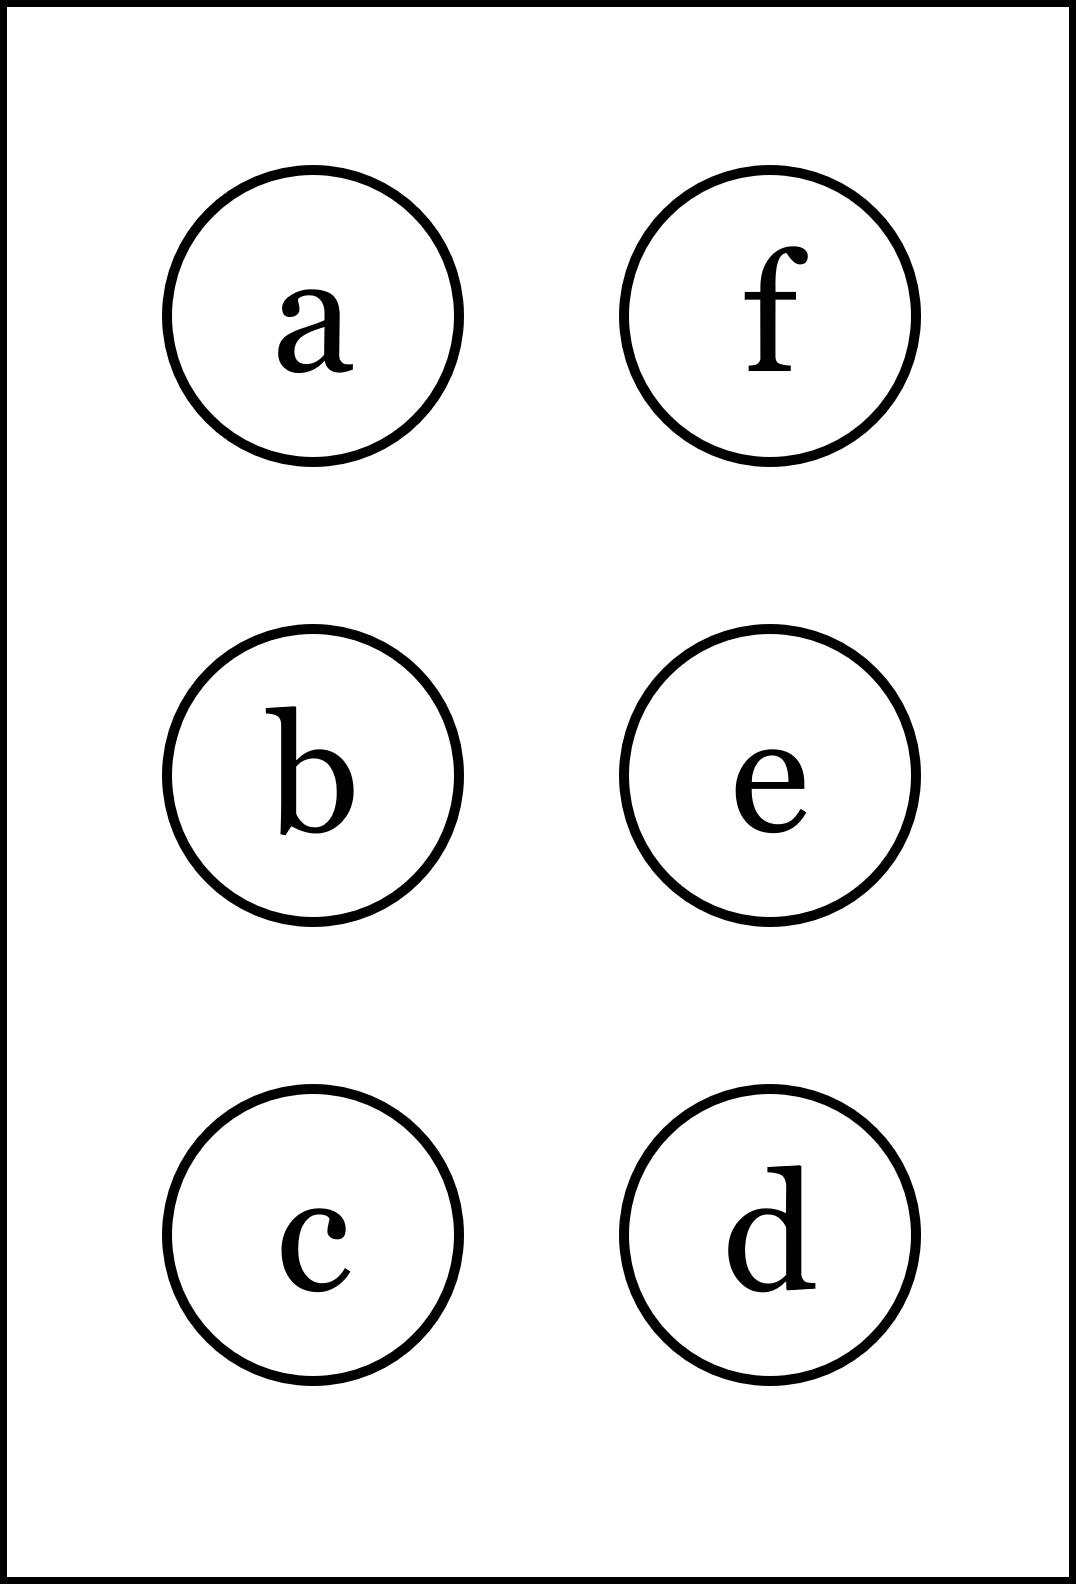
\includegraphics[height=40mm]{../images/braille.png}
{\small Písmeno Braillovej abecedy}
\end{center}
\end{minipage}
\end{center}
\end{minipage}
%
\end{tabular}
\newpage
\thispagestyle{empty}
\begin{tabular}{c:c}
\begin{minipage}[c][104.5mm][t]{0.5\linewidth}
\begin{center}
\vspace{7mm}
{\huge Volné extrémy, skupina \textit{Gamma $\gamma$} -\romannumeral1}\\[5mm]
\textit{Jméno:}\phantom{xxxxxxxxxxxxxxxxxxxxxxxxxxxxxxxxxxxxxxxxxxxxxxxxxxxxxxxxxxxxxxxxx}\\[5mm]
\begin{minipage}{0.95\linewidth}
\begin{center}
Cílem je najít \textbf{volné extrémy} funkce $f(x,y)$ zadané v \textbf{(a)}.\\Postupuj podle krokú v \textbf{(b)} až \textbf{(f)}. Pokud se medzivýsledky shodujú s těmi za otazníky,\\tak napravo obarvi příslušející kroužek načerno. \textbf{Spolu odevzdejte výsledné slovo}.
\end{center}
\end{minipage}
\\[1mm]
\begin{minipage}{0.79\linewidth}
\begin{center}
\begin{varwidth}{\linewidth}
\begin{enumerate}
\normalsize
\item $f(x,y)=-x^3+6x^2+15x-4-9y-6y^2-y^3$\quad \dotfill\; ???\;\dotfill \quad vybarvi
\item Najdi parciální derivaci podle $x$, $\pdv{f}{x}=$\quad \dotfill\; ???\;\dotfill \quad $-3x^2+12x+15$
\item Najdi stacionární body v $x$\quad \dotfill\; ???\;\dotfill \quad $x_1+x_2=4$
\item Najdi parciální derivaci podle $y$, $\pdv{f}{y}=$\quad \dotfill\; ???\;\dotfill \quad $-3y^2-12y-9$
\item Najdi stacionární body v $y$\quad \dotfill\; ???\;\dotfill \quad $y_1+y_2=-3$
\item Najdi funkční hodnoty vo všech stacionárních bodech \\ \phantom{xxxxxx} a vyber tu najvětší. $f_{\text{max}}(x,y)=$\quad \dotfill\; ???\;\dotfill \quad $-12$
\end{enumerate}
\end{varwidth}
\end{center}
\end{minipage}
\begin{minipage}{0.20\linewidth}
\begin{center}
{\Huge\bfseries 1.} \\[2mm]
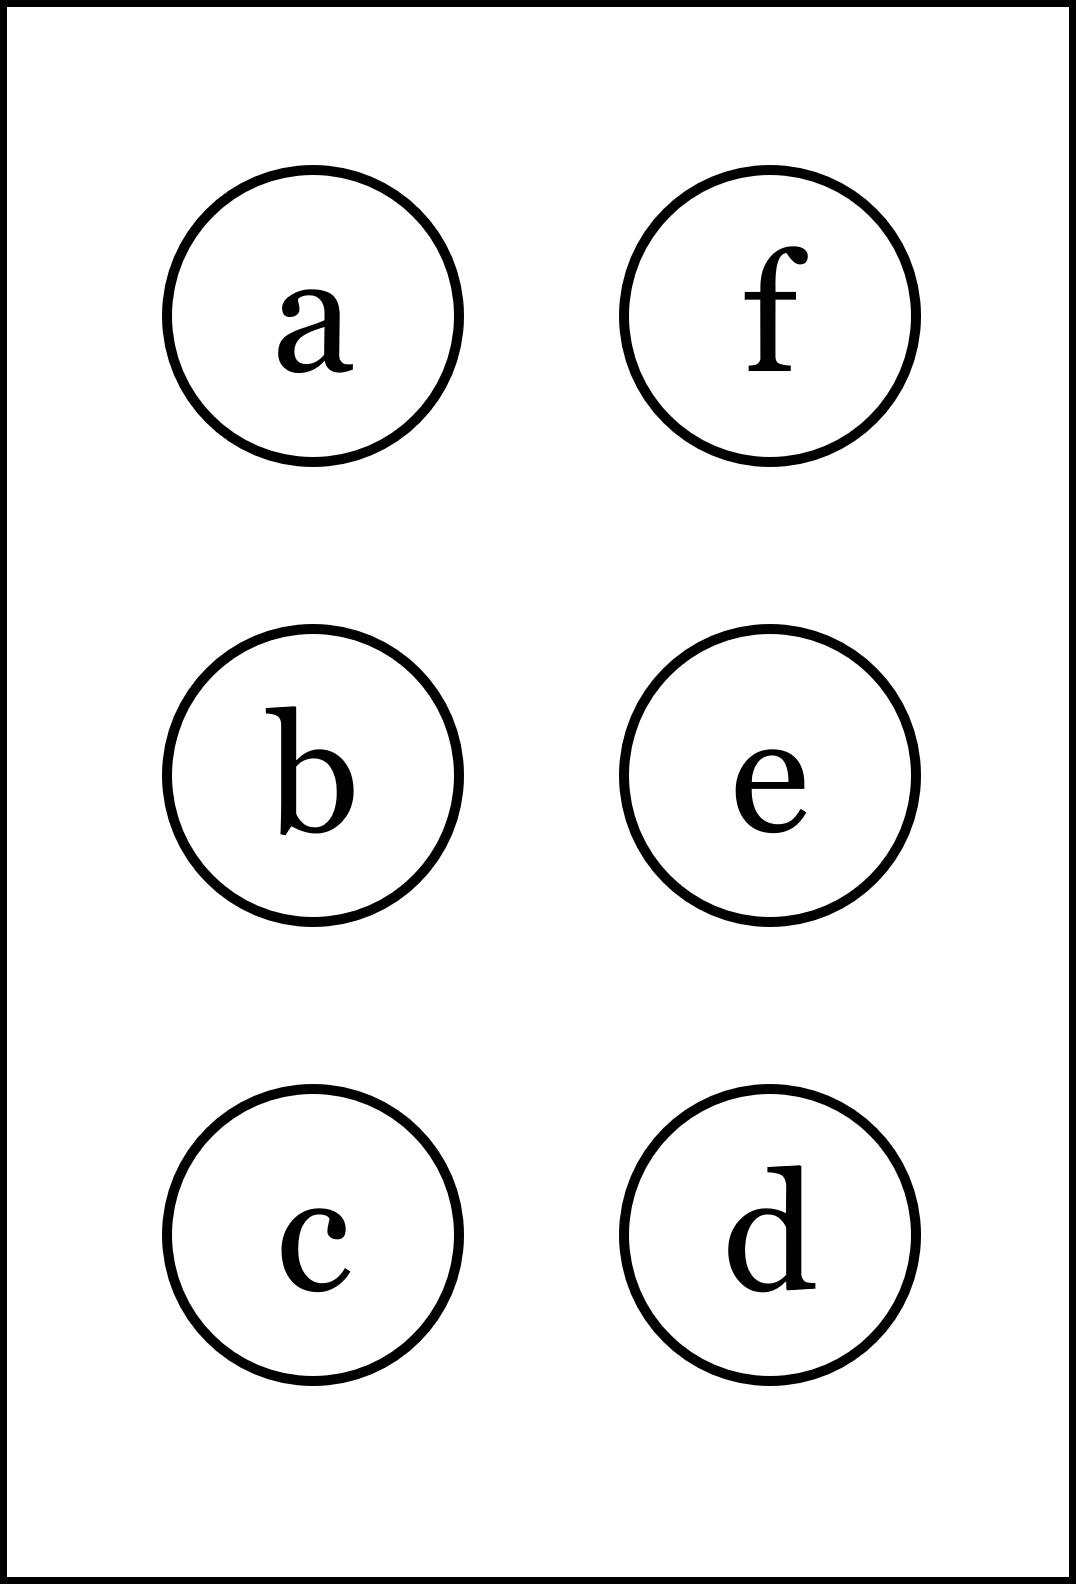
\includegraphics[height=40mm]{../images/braille.png}
{\small Písmeno Braillovej abecedy}
\end{center}
\end{minipage}
\end{center}
\end{minipage}
&
\begin{minipage}[c][104.5mm][t]{0.5\linewidth}
\begin{center}
\vspace{7mm}
{\huge Volné extrémy, skupina \textit{Gamma $\gamma$} -\romannumeral2}\\[5mm]
\textit{Jméno:}\phantom{xxxxxxxxxxxxxxxxxxxxxxxxxxxxxxxxxxxxxxxxxxxxxxxxxxxxxxxxxxxxxxxxx}\\[5mm]
\begin{minipage}{0.95\linewidth}
\begin{center}
Cílem je najít \textbf{volné extrémy} funkce $f(x,y)$ zadané v \textbf{(a)}.\\Postupuj podle krokú v \textbf{(b)} až \textbf{(f)}. Pokud se medzivýsledky shodujú s těmi za otazníky,\\tak napravo obarvi příslušející kroužek načerno. \textbf{Spolu odevzdejte výsledné slovo}.
\end{center}
\end{minipage}
\\[1mm]
\begin{minipage}{0.79\linewidth}
\begin{center}
\begin{varwidth}{\linewidth}
\begin{enumerate}
\normalsize
\item $f(x,y)=2x^3-12x^2-72x+4-24y+3y^2+y^3$\quad \dotfill\; ???\;\dotfill \quad vybarvi
\item Najdi parciální derivaci podle $x$, $\pdv{f}{x}=$\quad \dotfill\; ???\;\dotfill \quad $6x^2-12x-72$
\item Najdi stacionární body v $x$\quad \dotfill\; ???\;\dotfill \quad $x_1+x_2=5$
\item Najdi parciální derivaci podle $y$, $\pdv{f}{y}=$\quad \dotfill\; ???\;\dotfill \quad $3y^2+6y-18$
\item Najdi stacionární body v $y$\quad \dotfill\; ???\;\dotfill \quad $y_1+y_2=-1$
\item Najdi funkční hodnoty vo všech stacionárních bodech \\ \phantom{xxxxxx} a vyber tu najvětší. $f_{\text{max}}(x,y)=$\quad \dotfill\; ???\;\dotfill \quad $56$
\end{enumerate}
\end{varwidth}
\end{center}
\end{minipage}
\begin{minipage}{0.20\linewidth}
\begin{center}
{\Huge\bfseries 2.} \\[2mm]
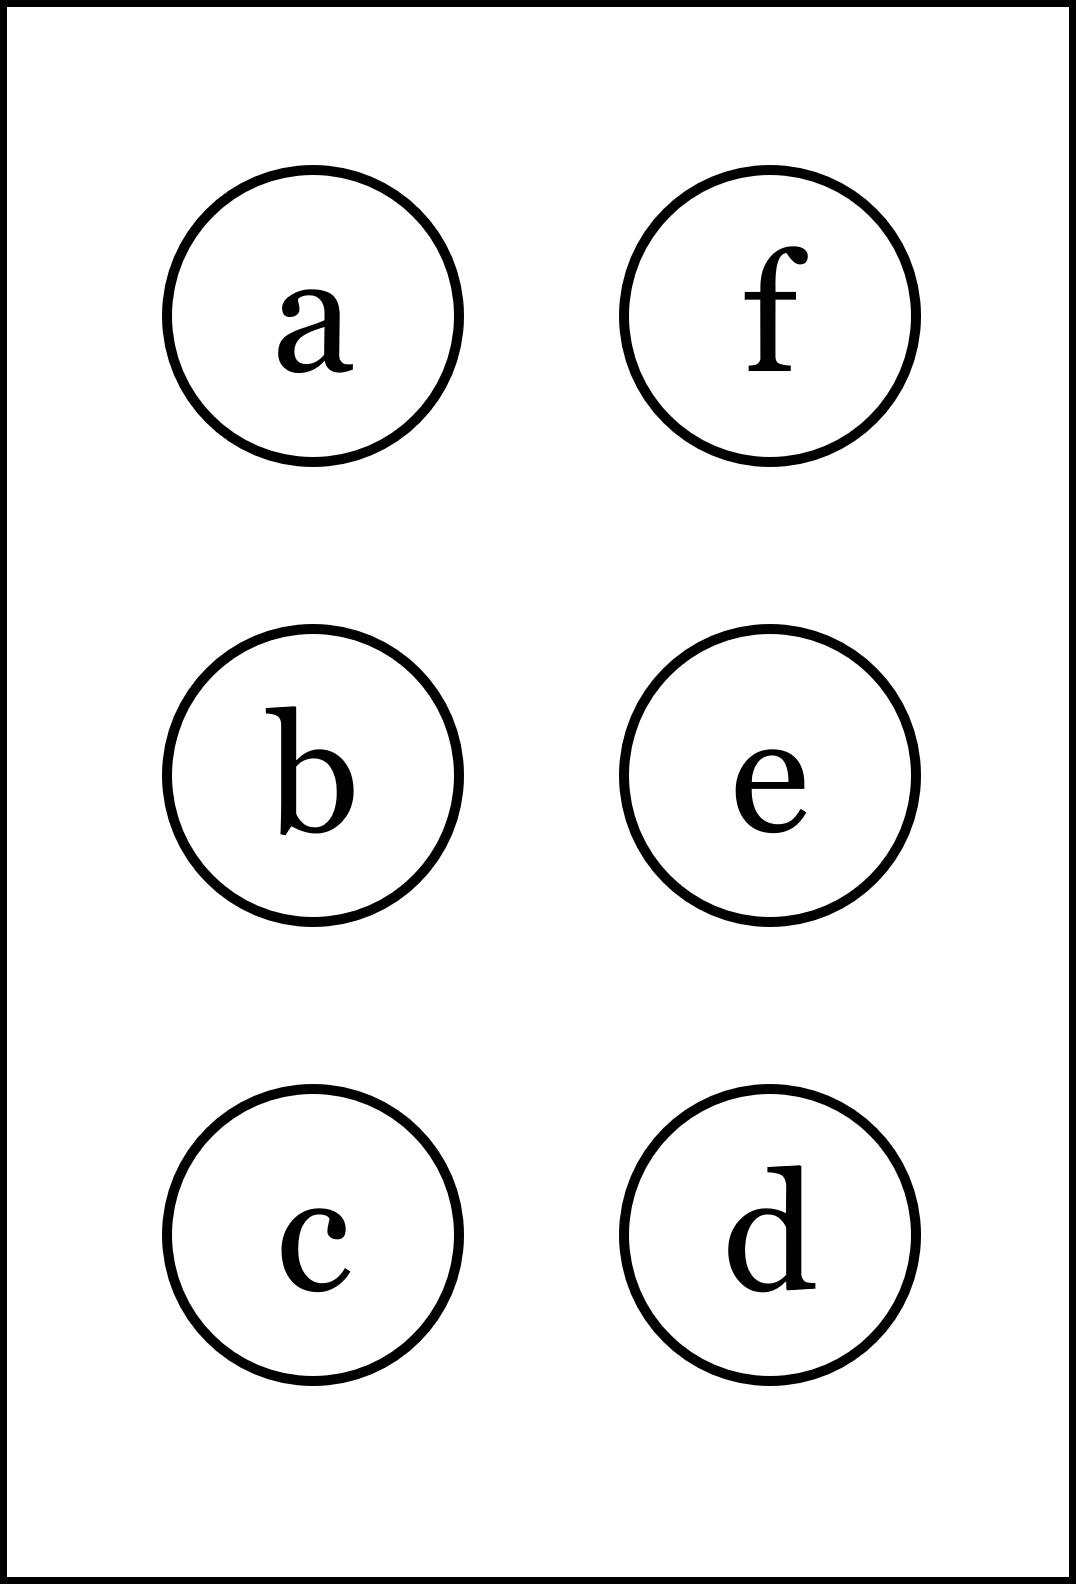
\includegraphics[height=40mm]{../images/braille.png}
{\small Písmeno Braillovej abecedy}
\end{center}
\end{minipage}
\end{center}
\end{minipage}
\\ \hdashline
\begin{minipage}[c][104.5mm][t]{0.5\linewidth}
\begin{center}
\vspace{7mm}
{\huge Volné extrémy, skupina \textit{Gamma $\gamma$} -\romannumeral3}\\[5mm]
\textit{Jméno:}\phantom{xxxxxxxxxxxxxxxxxxxxxxxxxxxxxxxxxxxxxxxxxxxxxxxxxxxxxxxxxxxxxxxxx}\\[5mm]
\begin{minipage}{0.95\linewidth}
\begin{center}
Cílem je najít \textbf{volné extrémy} funkce $f(x,y)$ zadané v \textbf{(a)}.\\Postupuj podle krokú v \textbf{(b)} až \textbf{(f)}. Pokud se medzivýsledky shodujú s těmi za otazníky,\\tak napravo obarvi příslušející kroužek načerno. \textbf{Spolu odevzdejte výsledné slovo}.
\end{center}
\end{minipage}
\\[1mm]
\begin{minipage}{0.79\linewidth}
\begin{center}
\begin{varwidth}{\linewidth}
\begin{enumerate}
\normalsize
\item $f(x,y)=-x^3-6x^2-9x-7+72y-12y^2-2y^3$\quad \dotfill\; ???\;\dotfill \quad vybarvi
\item Najdi parciální derivaci podle $x$, $\pdv{f}{x}=$\quad \dotfill\; ???\;\dotfill \quad $-3x^2-6x-9$
\item Najdi stacionární body v $x$\quad \dotfill\; ???\;\dotfill \quad $x_1+x_2=-4$
\item Najdi parciální derivaci podle $y$, $\pdv{f}{y}=$\quad \dotfill\; ???\;\dotfill \quad $-6y^2-24y+48$
\item Najdi stacionární body v $y$\quad \dotfill\; ???\;\dotfill \quad $y_1+y_2=-4$
\item Najdi funkční hodnoty vo všech stacionárních bodech \\ \phantom{xxxxxx} a vyber tu najvětší. $f_{\text{max}}(x,y)=$\quad \dotfill\; ???\;\dotfill \quad $77$
\end{enumerate}
\end{varwidth}
\end{center}
\end{minipage}
\begin{minipage}{0.20\linewidth}
\begin{center}
{\Huge\bfseries 3.} \\[2mm]
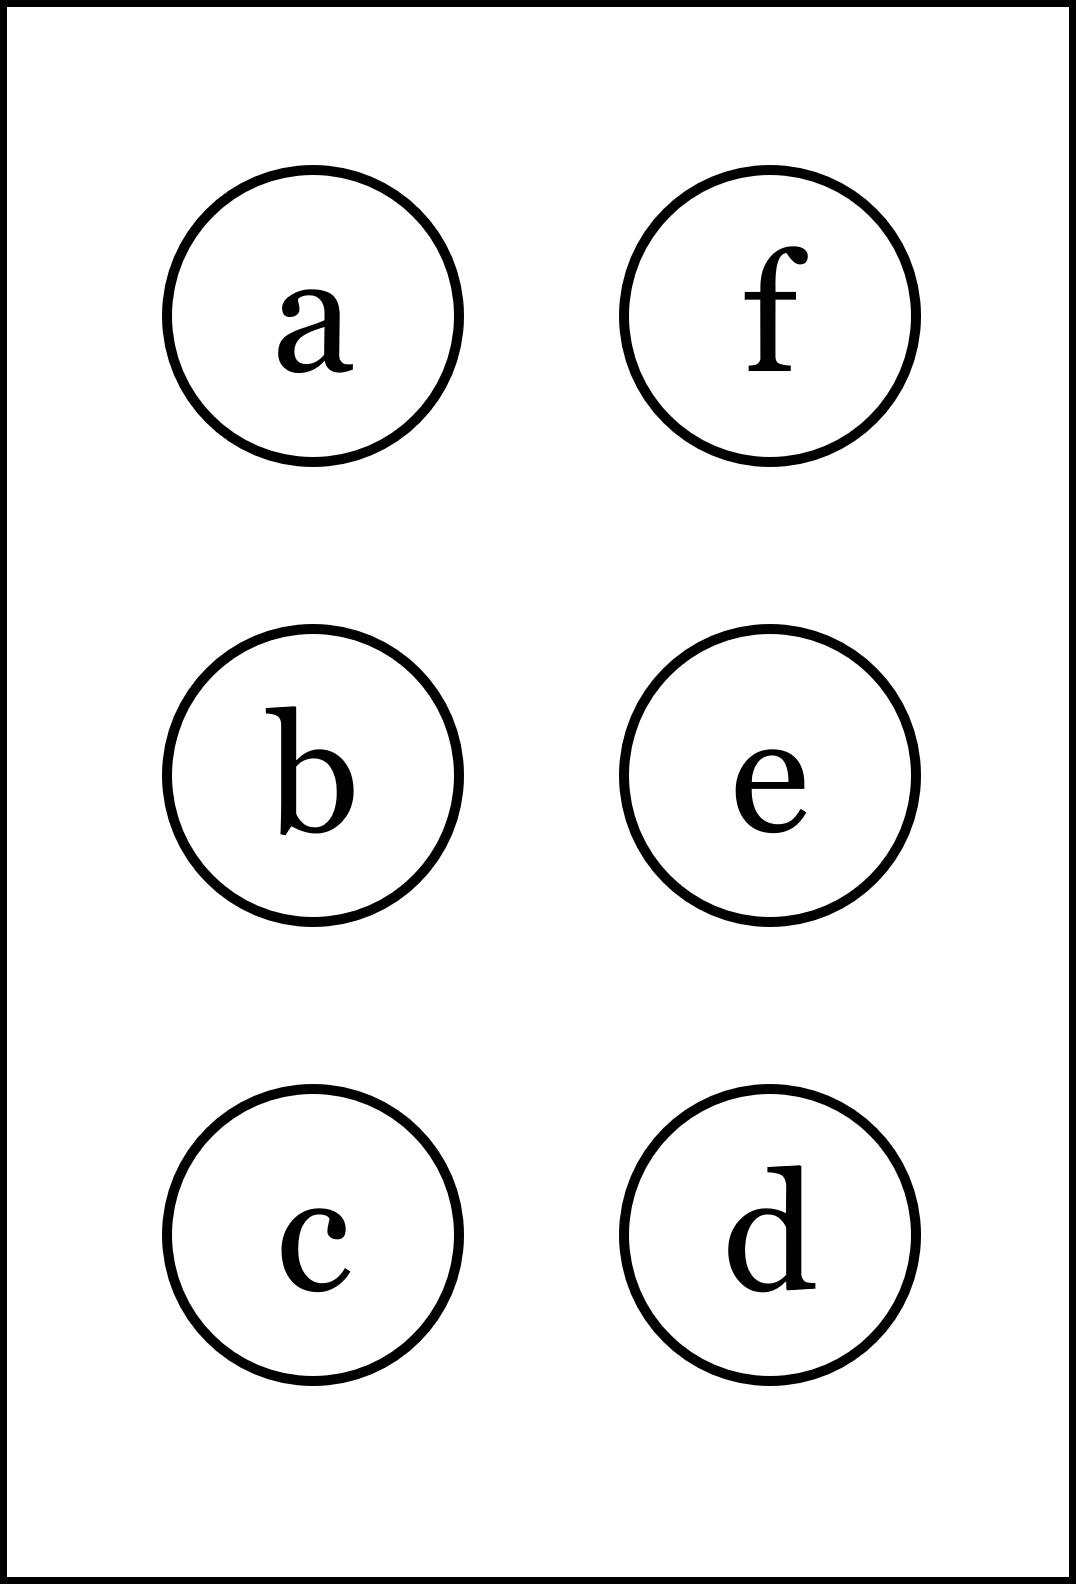
\includegraphics[height=40mm]{../images/braille.png}
{\small Písmeno Braillovej abecedy}
\end{center}
\end{minipage}
\end{center}
\end{minipage}
&
\begin{minipage}[c][104.5mm][t]{0.5\linewidth}
\begin{center}
\vspace{7mm}
{\huge Volné extrémy, skupina \textit{Gamma $\gamma$} -\romannumeral4}\\[5mm]
\textit{Jméno:}\phantom{xxxxxxxxxxxxxxxxxxxxxxxxxxxxxxxxxxxxxxxxxxxxxxxxxxxxxxxxxxxxxxxxx}\\[5mm]
\begin{minipage}{0.95\linewidth}
\begin{center}
Cílem je najít \textbf{volné extrémy} funkce $f(x,y)$ zadané v \textbf{(a)}.\\Postupuj podle krokú v \textbf{(b)} až \textbf{(f)}. Pokud se medzivýsledky shodujú s těmi za otazníky,\\tak napravo obarvi příslušející kroužek načerno. \textbf{Spolu odevzdejte výsledné slovo}.
\end{center}
\end{minipage}
\\[1mm]
\begin{minipage}{0.79\linewidth}
\begin{center}
\begin{varwidth}{\linewidth}
\begin{enumerate}
\normalsize
\item $f(x,y)=-2x^3+6x^2+18x-2+36y+6y^2-y^3$\quad \dotfill\; ???\;\dotfill \quad vybarvi
\item Najdi parciální derivaci podle $x$, $\pdv{f}{x}=$\quad \dotfill\; ???\;\dotfill \quad $-6x^2+6x+18$
\item Najdi stacionární body v $x$\quad \dotfill\; ???\;\dotfill \quad $x_1+x_2=3$
\item Najdi parciální derivaci podle $y$, $\pdv{f}{y}=$\quad \dotfill\; ???\;\dotfill \quad $-3y^2+12y+24$
\item Najdi stacionární body v $y$\quad \dotfill\; ???\;\dotfill \quad $y_1+y_2=5$
\item Najdi funkční hodnoty vo všech stacionárních bodech \\ \phantom{xxxxxx} a vyber tu najvětší. $f_{\text{max}}(x,y)=$\quad \dotfill\; ???\;\dotfill \quad $12$
\end{enumerate}
\end{varwidth}
\end{center}
\end{minipage}
\begin{minipage}{0.20\linewidth}
\begin{center}
{\Huge\bfseries 4.} \\[2mm]
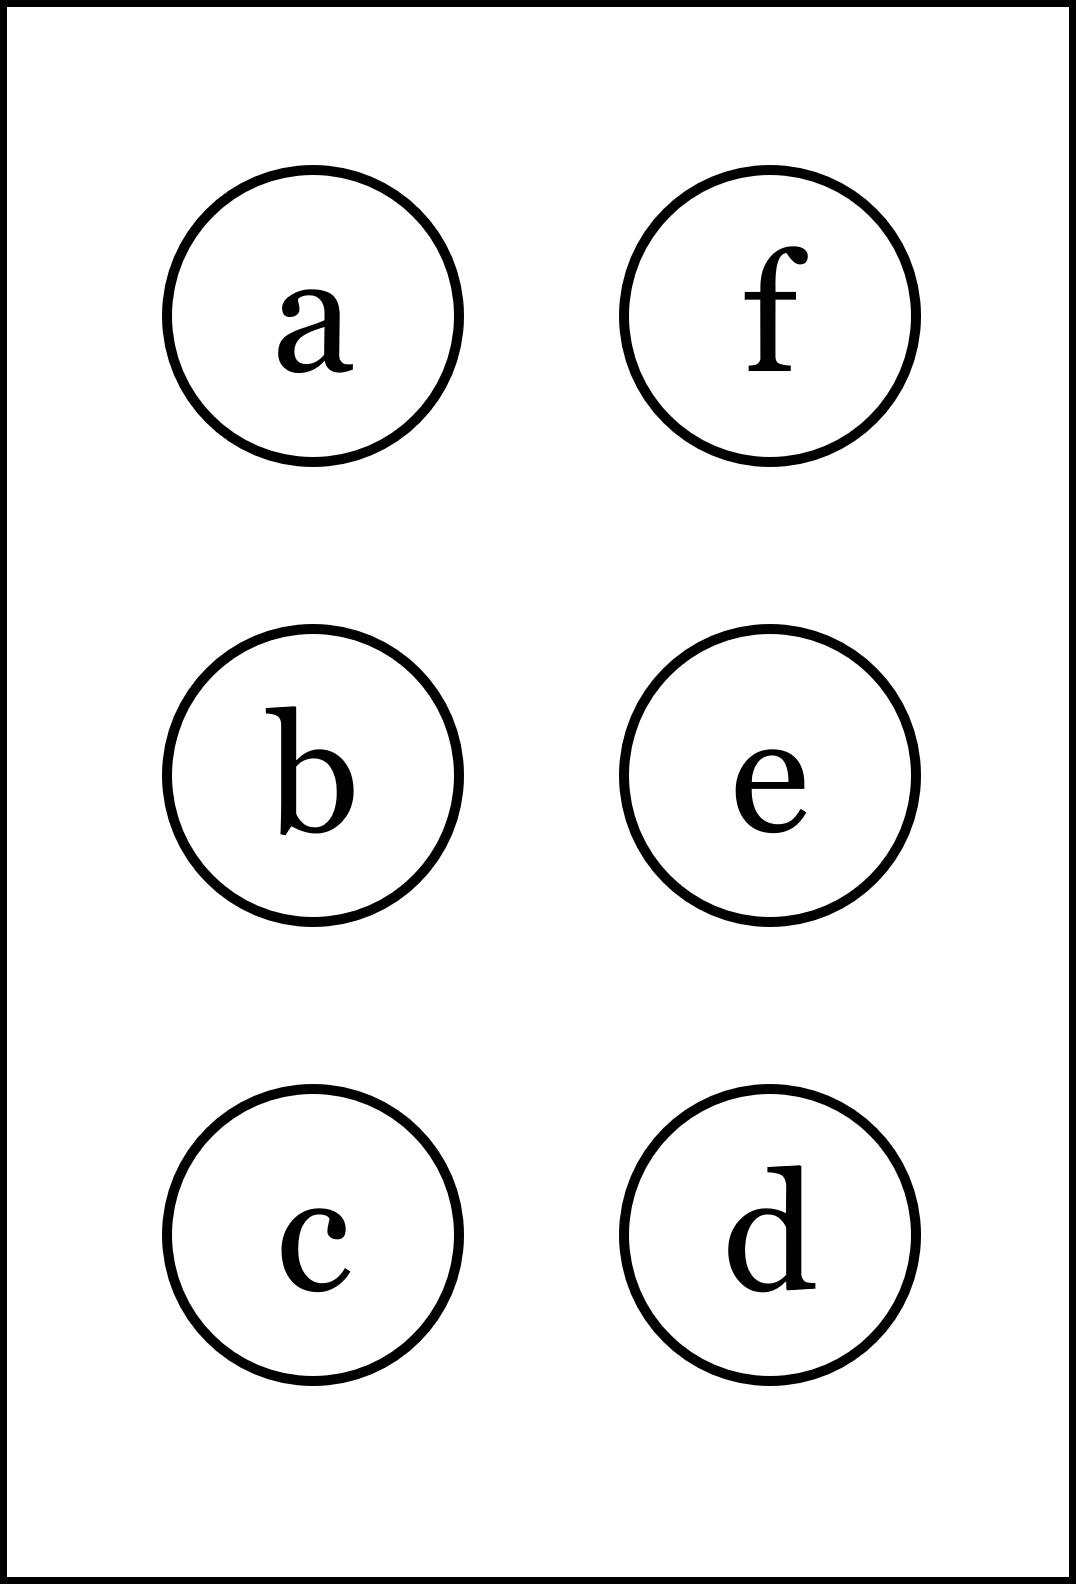
\includegraphics[height=40mm]{../images/braille.png}
{\small Písmeno Braillovej abecedy}
\end{center}
\end{minipage}
\end{center}
\end{minipage}
%
\end{tabular}
\newpage
\thispagestyle{empty}
\begin{tabular}{c:c}
\begin{minipage}[c][104.5mm][t]{0.5\linewidth}
\begin{center}
\vspace{7mm}
{\huge Volné extrémy, skupina \textit{Delta $\delta$} -\romannumeral1}\\[5mm]
\textit{Jméno:}\phantom{xxxxxxxxxxxxxxxxxxxxxxxxxxxxxxxxxxxxxxxxxxxxxxxxxxxxxxxxxxxxxxxxx}\\[5mm]
\begin{minipage}{0.95\linewidth}
\begin{center}
Cílem je najít \textbf{volné extrémy} funkce $f(x,y)$ zadané v \textbf{(a)}.\\Postupuj podle krokú v \textbf{(b)} až \textbf{(f)}. Pokud se medzivýsledky shodujú s těmi za otazníky,\\tak napravo obarvi příslušející kroužek načerno. \textbf{Spolu odevzdejte výsledné slovo}.
\end{center}
\end{minipage}
\\[1mm]
\begin{minipage}{0.79\linewidth}
\begin{center}
\begin{varwidth}{\linewidth}
\begin{enumerate}
\normalsize
\item $f(x,y)=-7x^3-21x^2+63x+4-45y-3y^2+y^3$\quad \dotfill\; ???\;\dotfill \quad vybarvi
\item Najdi parciální derivaci podle $x$, $\pdv{f}{x}=$\quad \dotfill\; ???\;\dotfill \quad $-21x^2-21x+63$
\item Najdi stacionární body v $x$\quad \dotfill\; ???\;\dotfill \quad $x_1+x_2=-2$
\item Najdi parciální derivaci podle $y$, $\pdv{f}{y}=$\quad \dotfill\; ???\;\dotfill \quad $3y^2-6y-36$
\item Najdi stacionární body v $y$\quad \dotfill\; ???\;\dotfill \quad $y_1+y_2=2$
\item Najdi funkční hodnoty vo všech stacionárních bodech \\ \phantom{xxxxxx} a vyber tu najvětší. $f_{\text{max}}(x,y)=$\quad \dotfill\; ???\;\dotfill \quad $-360$
\end{enumerate}
\end{varwidth}
\end{center}
\end{minipage}
\begin{minipage}{0.20\linewidth}
\begin{center}
{\Huge\bfseries 1.} \\[2mm]
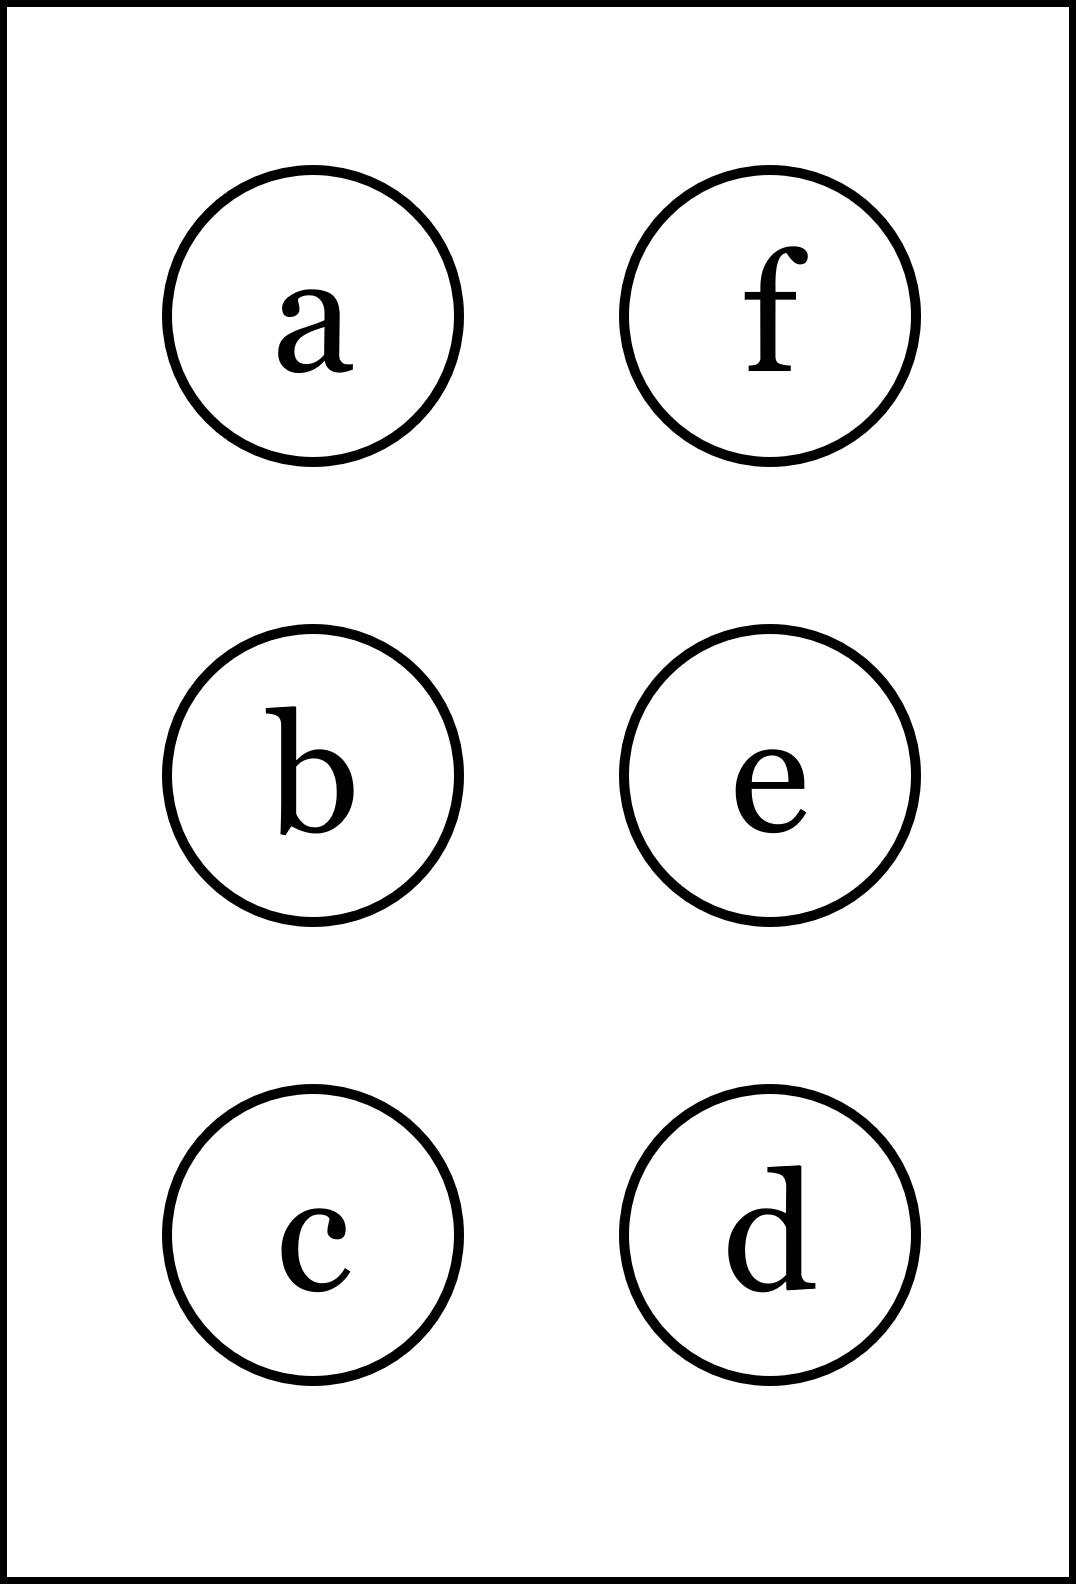
\includegraphics[height=40mm]{../images/braille.png}
{\small Písmeno Braillovej abecedy}
\end{center}
\end{minipage}
\end{center}
\end{minipage}
&
\begin{minipage}[c][104.5mm][t]{0.5\linewidth}
\begin{center}
\vspace{7mm}
{\huge Volné extrémy, skupina \textit{Delta $\delta$} -\romannumeral2}\\[5mm]
\textit{Jméno:}\phantom{xxxxxxxxxxxxxxxxxxxxxxxxxxxxxxxxxxxxxxxxxxxxxxxxxxxxxxxxxxxxxxxxx}\\[5mm]
\begin{minipage}{0.95\linewidth}
\begin{center}
Cílem je najít \textbf{volné extrémy} funkce $f(x,y)$ zadané v \textbf{(a)}.\\Postupuj podle krokú v \textbf{(b)} až \textbf{(f)}. Pokud se medzivýsledky shodujú s těmi za otazníky,\\tak napravo obarvi příslušející kroužek načerno. \textbf{Spolu odevzdejte výsledné slovo}.
\end{center}
\end{minipage}
\\[1mm]
\begin{minipage}{0.79\linewidth}
\begin{center}
\begin{varwidth}{\linewidth}
\begin{enumerate}
\normalsize
\item $f(x,y)=-x^3+9x^2+21x-3-15y-9y^2-y^3$\quad \dotfill\; ???\;\dotfill \quad nebarvi
\item Najdi parciální derivaci podle $x$, $\pdv{f}{x}=$\quad \dotfill\; ???\;\dotfill \quad $-3x^2+18x+21$
\item Najdi stacionární body v $x$\quad \dotfill\; ???\;\dotfill \quad $x_1+x_2=6$
\item Najdi parciální derivaci podle $y$, $\pdv{f}{y}=$\quad \dotfill\; ???\;\dotfill \quad $-3y^2-18y-6$
\item Najdi stacionární body v $y$\quad \dotfill\; ???\;\dotfill \quad $y_1+y_2=-5$
\item Najdi funkční hodnoty vo všech stacionárních bodech \\ \phantom{xxxxxx} a vyber tu najvětší. $f_{\text{max}}(x,y)=$\quad \dotfill\; ???\;\dotfill \quad $249$
\end{enumerate}
\end{varwidth}
\end{center}
\end{minipage}
\begin{minipage}{0.20\linewidth}
\begin{center}
{\Huge\bfseries 2.} \\[2mm]
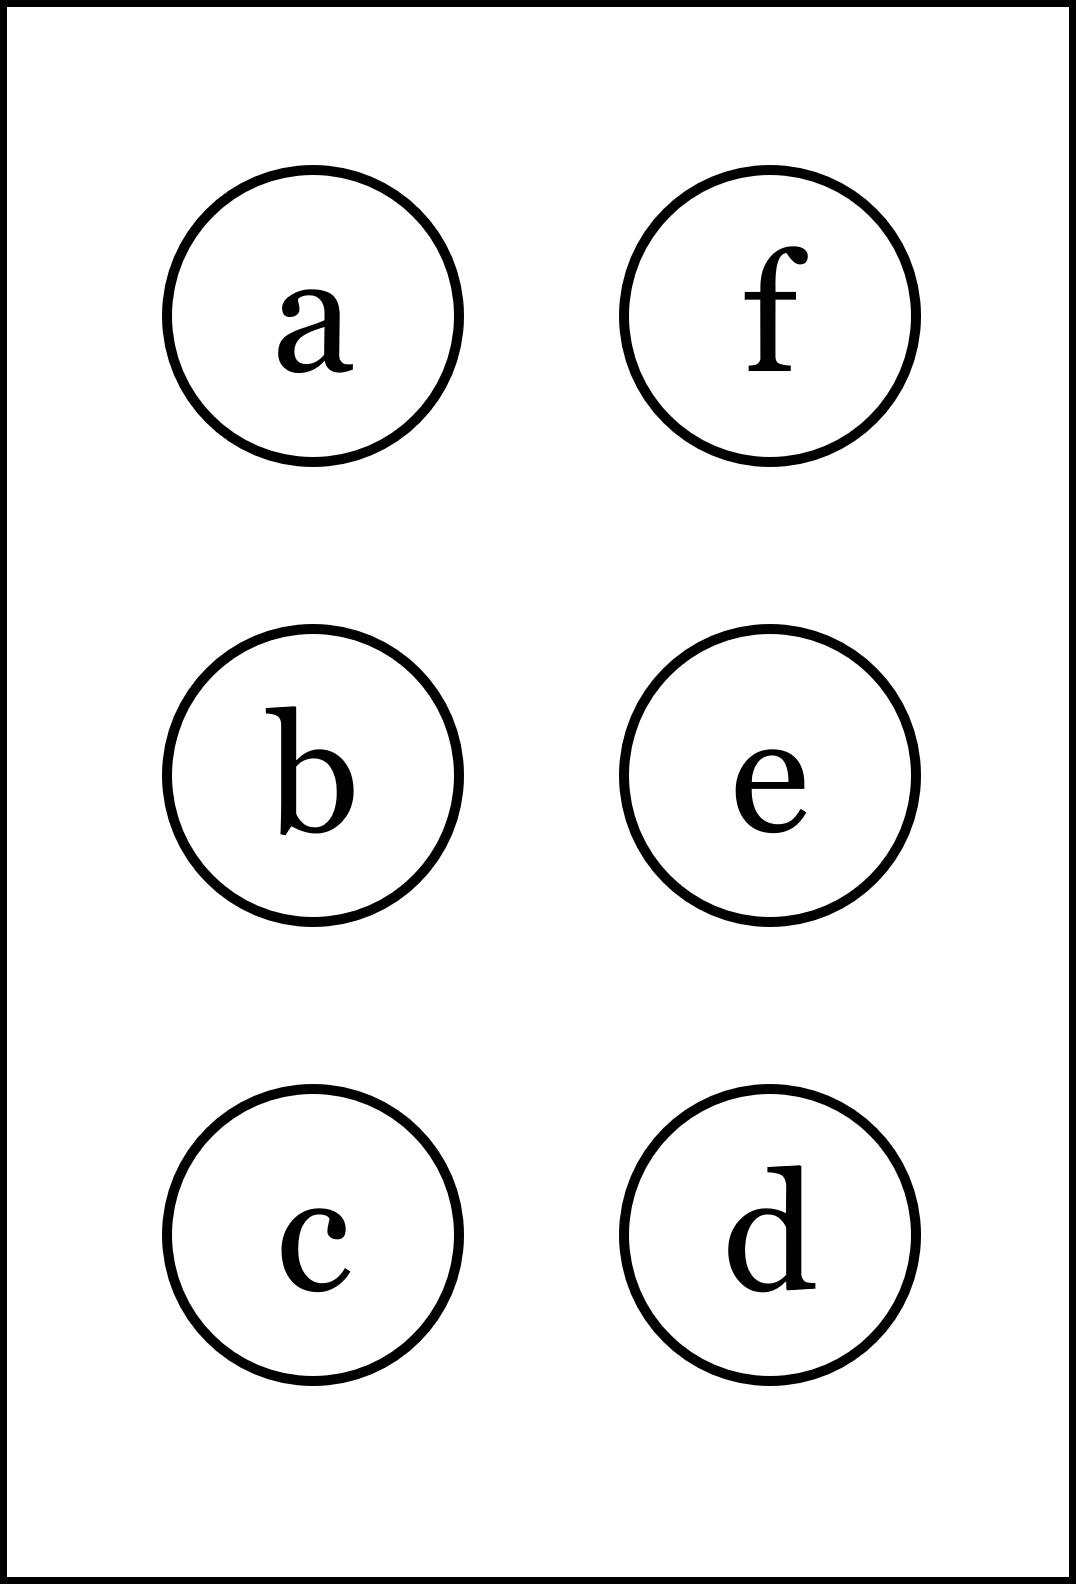
\includegraphics[height=40mm]{../images/braille.png}
{\small Písmeno Braillovej abecedy}
\end{center}
\end{minipage}
\end{center}
\end{minipage}
\\ \hdashline
\begin{minipage}[c][104.5mm][t]{0.5\linewidth}
\begin{center}
\vspace{7mm}
{\huge Volné extrémy, skupina \textit{Delta $\delta$} -\romannumeral3}\\[5mm]
\textit{Jméno:}\phantom{xxxxxxxxxxxxxxxxxxxxxxxxxxxxxxxxxxxxxxxxxxxxxxxxxxxxxxxxxxxxxxxxx}\\[5mm]
\begin{minipage}{0.95\linewidth}
\begin{center}
Cílem je najít \textbf{volné extrémy} funkce $f(x,y)$ zadané v \textbf{(a)}.\\Postupuj podle krokú v \textbf{(b)} až \textbf{(f)}. Pokud se medzivýsledky shodujú s těmi za otazníky,\\tak napravo obarvi příslušející kroužek načerno. \textbf{Spolu odevzdejte výsledné slovo}.
\end{center}
\end{minipage}
\\[1mm]
\begin{minipage}{0.79\linewidth}
\begin{center}
\begin{varwidth}{\linewidth}
\begin{enumerate}
\normalsize
\item $f(x,y)=2x^3+12x^2+18x+5+54y-18y^2-6y^3$\quad \dotfill\; ???\;\dotfill \quad vybarvi
\item Najdi parciální derivaci podle $x$, $\pdv{f}{x}=$\quad \dotfill\; ???\;\dotfill \quad $6x^2+12x+18$
\item Najdi stacionární body v $x$\quad \dotfill\; ???\;\dotfill \quad $x_1+x_2=-3$
\item Najdi parciální derivaci podle $y$, $\pdv{f}{y}=$\quad \dotfill\; ???\;\dotfill \quad $-18y^2-36y+36$
\item Najdi stacionární body v $y$\quad \dotfill\; ???\;\dotfill \quad $y_1+y_2=-2$
\item Najdi funkční hodnoty vo všech stacionárních bodech \\ \phantom{xxxxxx} a vyber tu najvětší. $f_{\text{max}}(x,y)=$\quad \dotfill\; ???\;\dotfill \quad $-165$
\end{enumerate}
\end{varwidth}
\end{center}
\end{minipage}
\begin{minipage}{0.20\linewidth}
\begin{center}
{\Huge\bfseries 3.} \\[2mm]
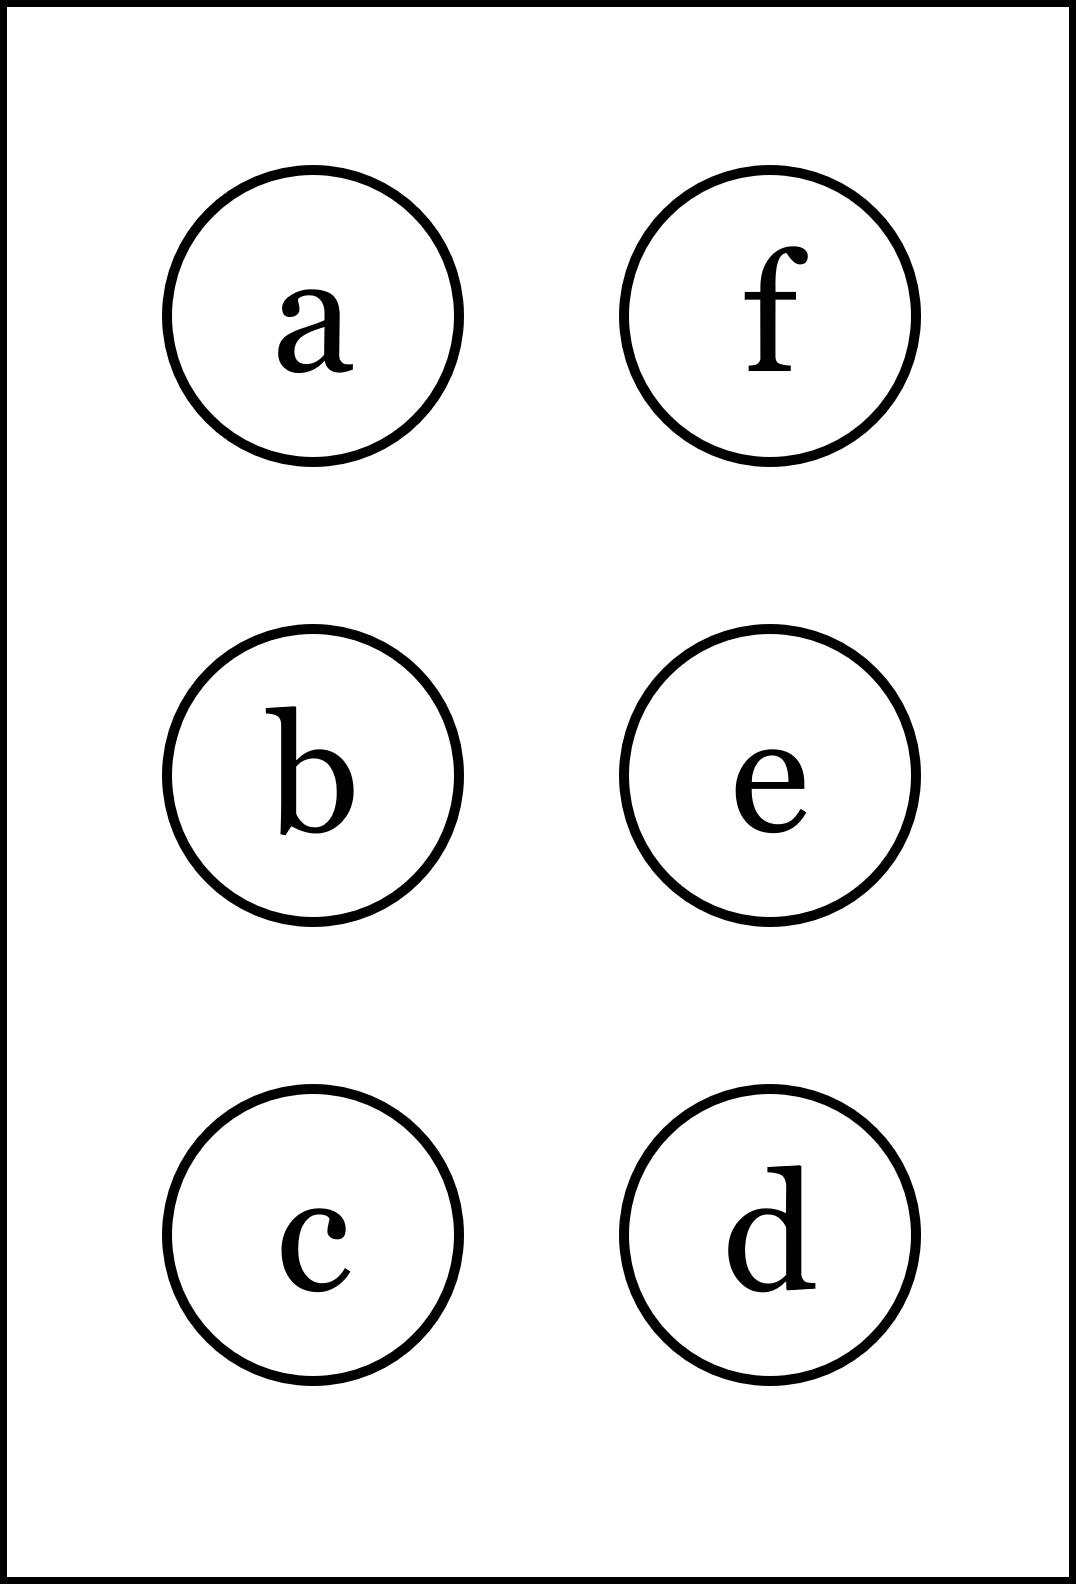
\includegraphics[height=40mm]{../images/braille.png}
{\small Písmeno Braillovej abecedy}
\end{center}
\end{minipage}
\end{center}
\end{minipage}
&
\begin{minipage}[c][104.5mm][t]{0.5\linewidth}
\begin{center}
\vspace{7mm}
{\huge Volné extrémy, skupina \textit{Delta $\delta$} -\romannumeral4}\\[5mm]
\textit{Jméno:}\phantom{xxxxxxxxxxxxxxxxxxxxxxxxxxxxxxxxxxxxxxxxxxxxxxxxxxxxxxxxxxxxxxxxx}\\[5mm]
\begin{minipage}{0.95\linewidth}
\begin{center}
Cílem je najít \textbf{volné extrémy} funkce $f(x,y)$ zadané v \textbf{(a)}.\\Postupuj podle krokú v \textbf{(b)} až \textbf{(f)}. Pokud se medzivýsledky shodujú s těmi za otazníky,\\tak napravo obarvi příslušející kroužek načerno. \textbf{Spolu odevzdejte výsledné slovo}.
\end{center}
\end{minipage}
\\[1mm]
\begin{minipage}{0.79\linewidth}
\begin{center}
\begin{varwidth}{\linewidth}
\begin{enumerate}
\normalsize
\item $f(x,y)=-4x^3+12x^2+36x+1-75y+30y^2+5y^3$\quad \dotfill\; ???\;\dotfill \quad vybarvi
\item Najdi parciální derivaci podle $x$, $\pdv{f}{x}=$\quad \dotfill\; ???\;\dotfill \quad $-12x^2+24x+36$
\item Najdi stacionární body v $x$\quad \dotfill\; ???\;\dotfill \quad $x_1+x_2=2$
\item Najdi parciální derivaci podle $y$, $\pdv{f}{y}=$\quad \dotfill\; ???\;\dotfill \quad $15y^2+60y-45$
\item Najdi stacionární body v $y$\quad \dotfill\; ???\;\dotfill \quad $y_1+y_2=-3$
\item Najdi funkční hodnoty vo všech stacionárních bodech \\ \phantom{xxxxxx} a vyber tu najvětší. $f_{\text{max}}(x,y)=$\quad \dotfill\; ???\;\dotfill \quad $69$
\end{enumerate}
\end{varwidth}
\end{center}
\end{minipage}
\begin{minipage}{0.20\linewidth}
\begin{center}
{\Huge\bfseries 4.} \\[2mm]
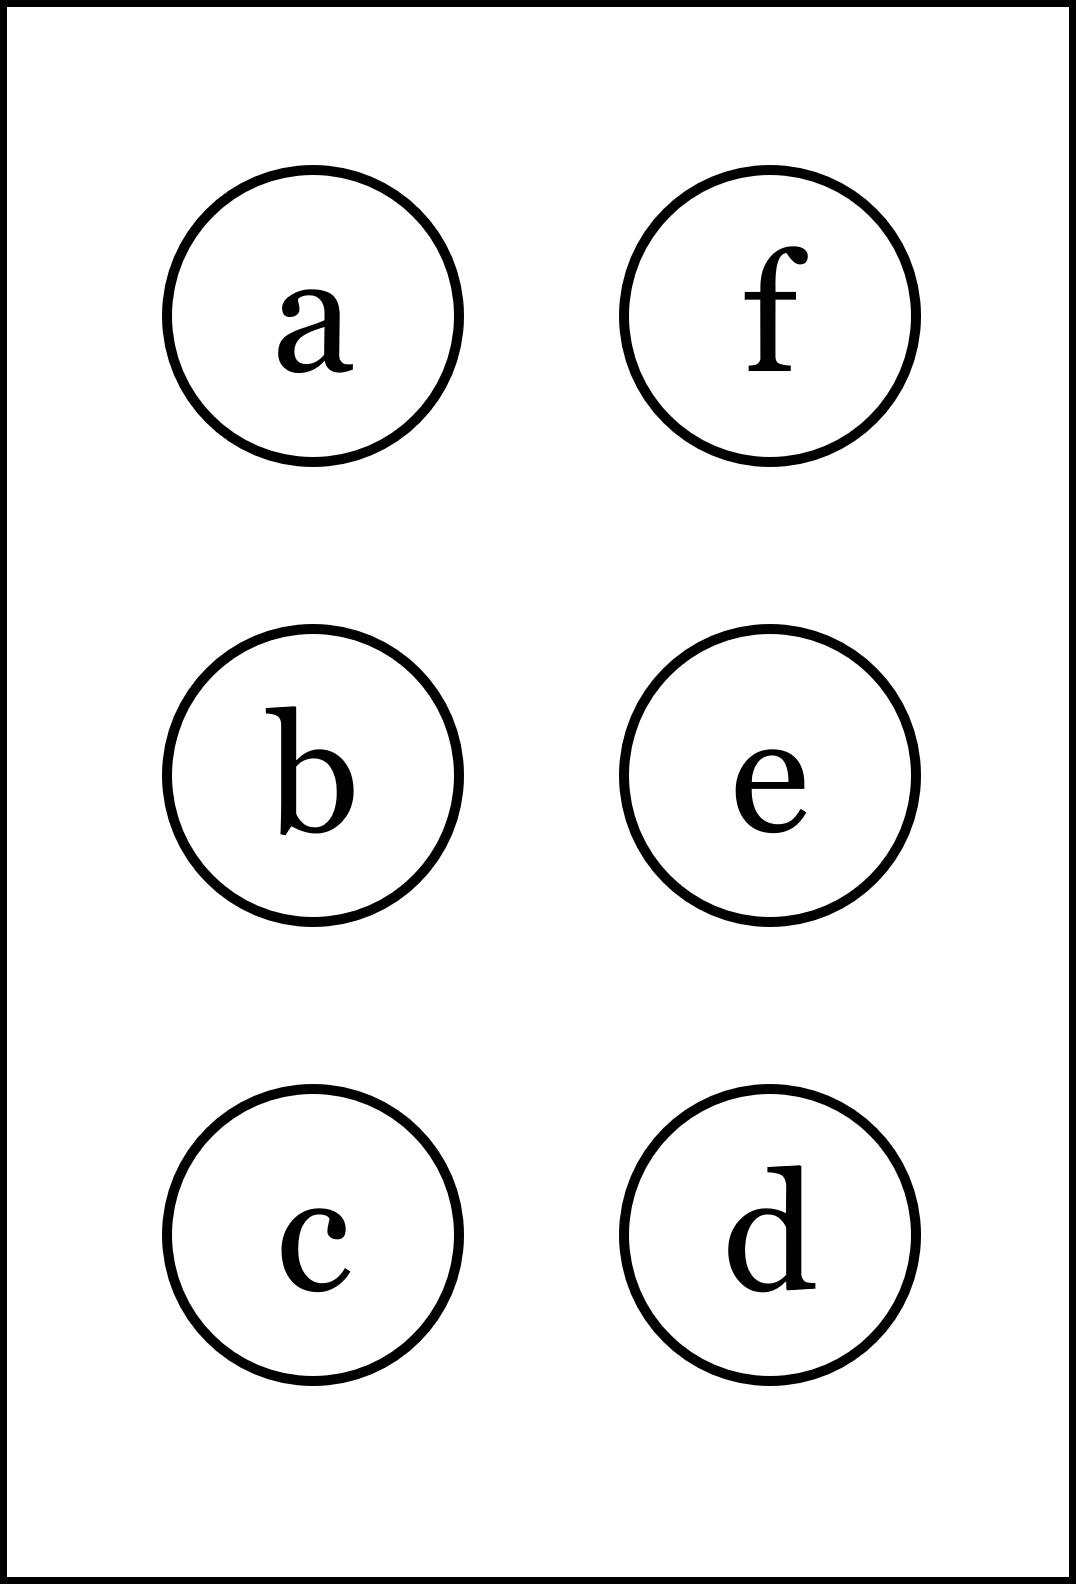
\includegraphics[height=40mm]{../images/braille.png}
{\small Písmeno Braillovej abecedy}
\end{center}
\end{minipage}
\end{center}
\end{minipage}
%
\end{tabular}
\newpage
\thispagestyle{empty}
\begin{tabular}{c:c}
\begin{minipage}[c][104.5mm][t]{0.5\linewidth}
\begin{center}
\vspace{7mm}
{\huge Volné extrémy, skupina \textit{Epsilon $\epsilon$} -\romannumeral1}\\[5mm]
\textit{Jméno:}\phantom{xxxxxxxxxxxxxxxxxxxxxxxxxxxxxxxxxxxxxxxxxxxxxxxxxxxxxxxxxxxxxxxxx}\\[5mm]
\begin{minipage}{0.95\linewidth}
\begin{center}
Cílem je najít \textbf{volné extrémy} funkce $f(x,y)$ zadané v \textbf{(a)}.\\Postupuj podle krokú v \textbf{(b)} až \textbf{(f)}. Pokud se medzivýsledky shodujú s těmi za otazníky,\\tak napravo obarvi příslušející kroužek načerno. \textbf{Spolu odevzdejte výsledné slovo}.
\end{center}
\end{minipage}
\\[1mm]
\begin{minipage}{0.79\linewidth}
\begin{center}
\begin{varwidth}{\linewidth}
\begin{enumerate}
\normalsize
\item $f(x,y)=4x^3+12x^2-36x+3-45y-30y^2-5y^3$\quad \dotfill\; ???\;\dotfill \quad vybarvi
\item Najdi parciální derivaci podle $x$, $\pdv{f}{x}=$\quad \dotfill\; ???\;\dotfill \quad $12x^2+24x-36$
\item Najdi stacionární body v $x$\quad \dotfill\; ???\;\dotfill \quad $x_1+x_2=-1$
\item Najdi parciální derivaci podle $y$, $\pdv{f}{y}=$\quad \dotfill\; ???\;\dotfill \quad $-15y^2-60y-15$
\item Najdi stacionární body v $y$\quad \dotfill\; ???\;\dotfill \quad $y_1+y_2=-3$
\item Najdi funkční hodnoty vo všech stacionárních bodech \\ \phantom{xxxxxx} a vyber tu najvětší. $f_{\text{max}}(x,y)=$\quad \dotfill\; ???\;\dotfill \quad $-17$
\end{enumerate}
\end{varwidth}
\end{center}
\end{minipage}
\begin{minipage}{0.20\linewidth}
\begin{center}
{\Huge\bfseries 1.} \\[2mm]
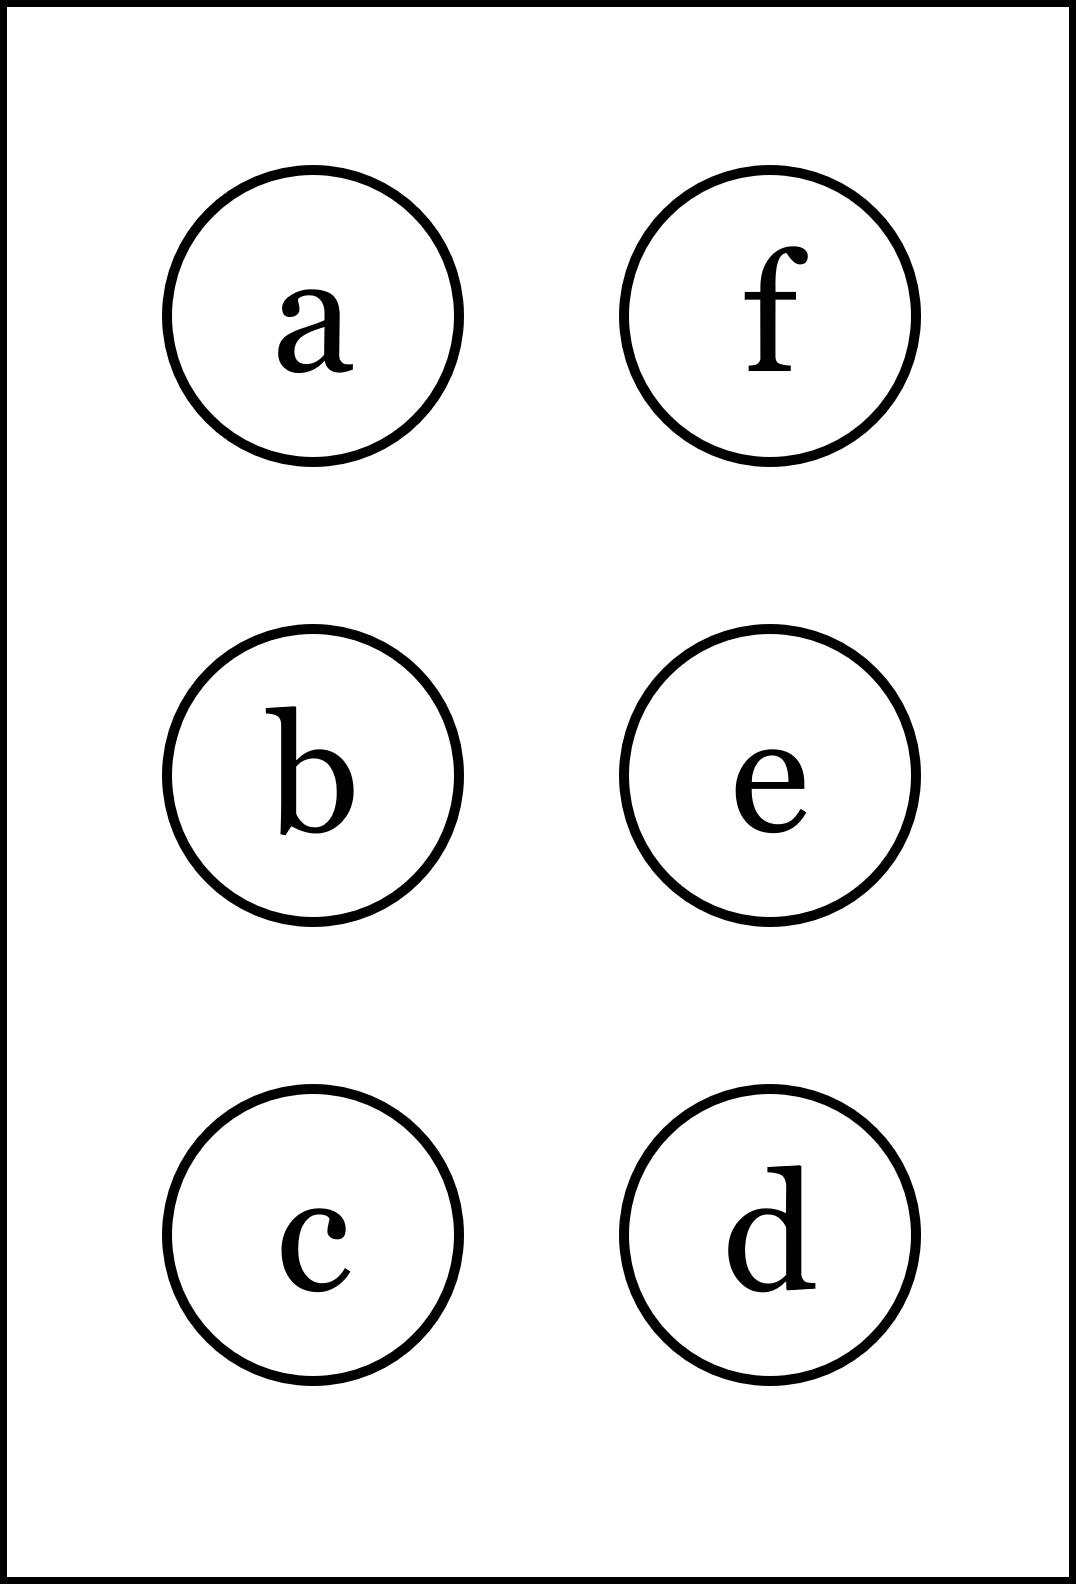
\includegraphics[height=40mm]{../images/braille.png}
{\small Písmeno Braillovej abecedy}
\end{center}
\end{minipage}
\end{center}
\end{minipage}
&
\begin{minipage}[c][104.5mm][t]{0.5\linewidth}
\begin{center}
\vspace{7mm}
{\huge Volné extrémy, skupina \textit{Epsilon $\epsilon$} -\romannumeral2}\\[5mm]
\textit{Jméno:}\phantom{xxxxxxxxxxxxxxxxxxxxxxxxxxxxxxxxxxxxxxxxxxxxxxxxxxxxxxxxxxxxxxxxx}\\[5mm]
\begin{minipage}{0.95\linewidth}
\begin{center}
Cílem je najít \textbf{volné extrémy} funkce $f(x,y)$ zadané v \textbf{(a)}.\\Postupuj podle krokú v \textbf{(b)} až \textbf{(f)}. Pokud se medzivýsledky shodujú s těmi za otazníky,\\tak napravo obarvi příslušející kroužek načerno. \textbf{Spolu odevzdejte výsledné slovo}.
\end{center}
\end{minipage}
\\[1mm]
\begin{minipage}{0.79\linewidth}
\begin{center}
\begin{varwidth}{\linewidth}
\begin{enumerate}
\normalsize
\item $f(x,y)=-x^3+9x^2+21x-6-9y-3y^2+y^3$\quad \dotfill\; ???\;\dotfill \quad vybarvi
\item Najdi parciální derivaci podle $x$, $\pdv{f}{x}=$\quad \dotfill\; ???\;\dotfill \quad $-3x^2+9x+21$
\item Najdi stacionární body v $x$\quad \dotfill\; ???\;\dotfill \quad $x_1+x_2=7$
\item Najdi parciální derivaci podle $y$, $\pdv{f}{y}=$\quad \dotfill\; ???\;\dotfill \quad $3y^2-6y-9$
\item Najdi stacionární body v $y$\quad \dotfill\; ???\;\dotfill \quad $y_1+y_2=3$
\item Najdi funkční hodnoty vo všech stacionárních bodech \\ \phantom{xxxxxx} a vyber tu najvětší. $f_{\text{max}}(x,y)=$\quad \dotfill\; ???\;\dotfill \quad $212$
\end{enumerate}
\end{varwidth}
\end{center}
\end{minipage}
\begin{minipage}{0.20\linewidth}
\begin{center}
{\Huge\bfseries 2.} \\[2mm]
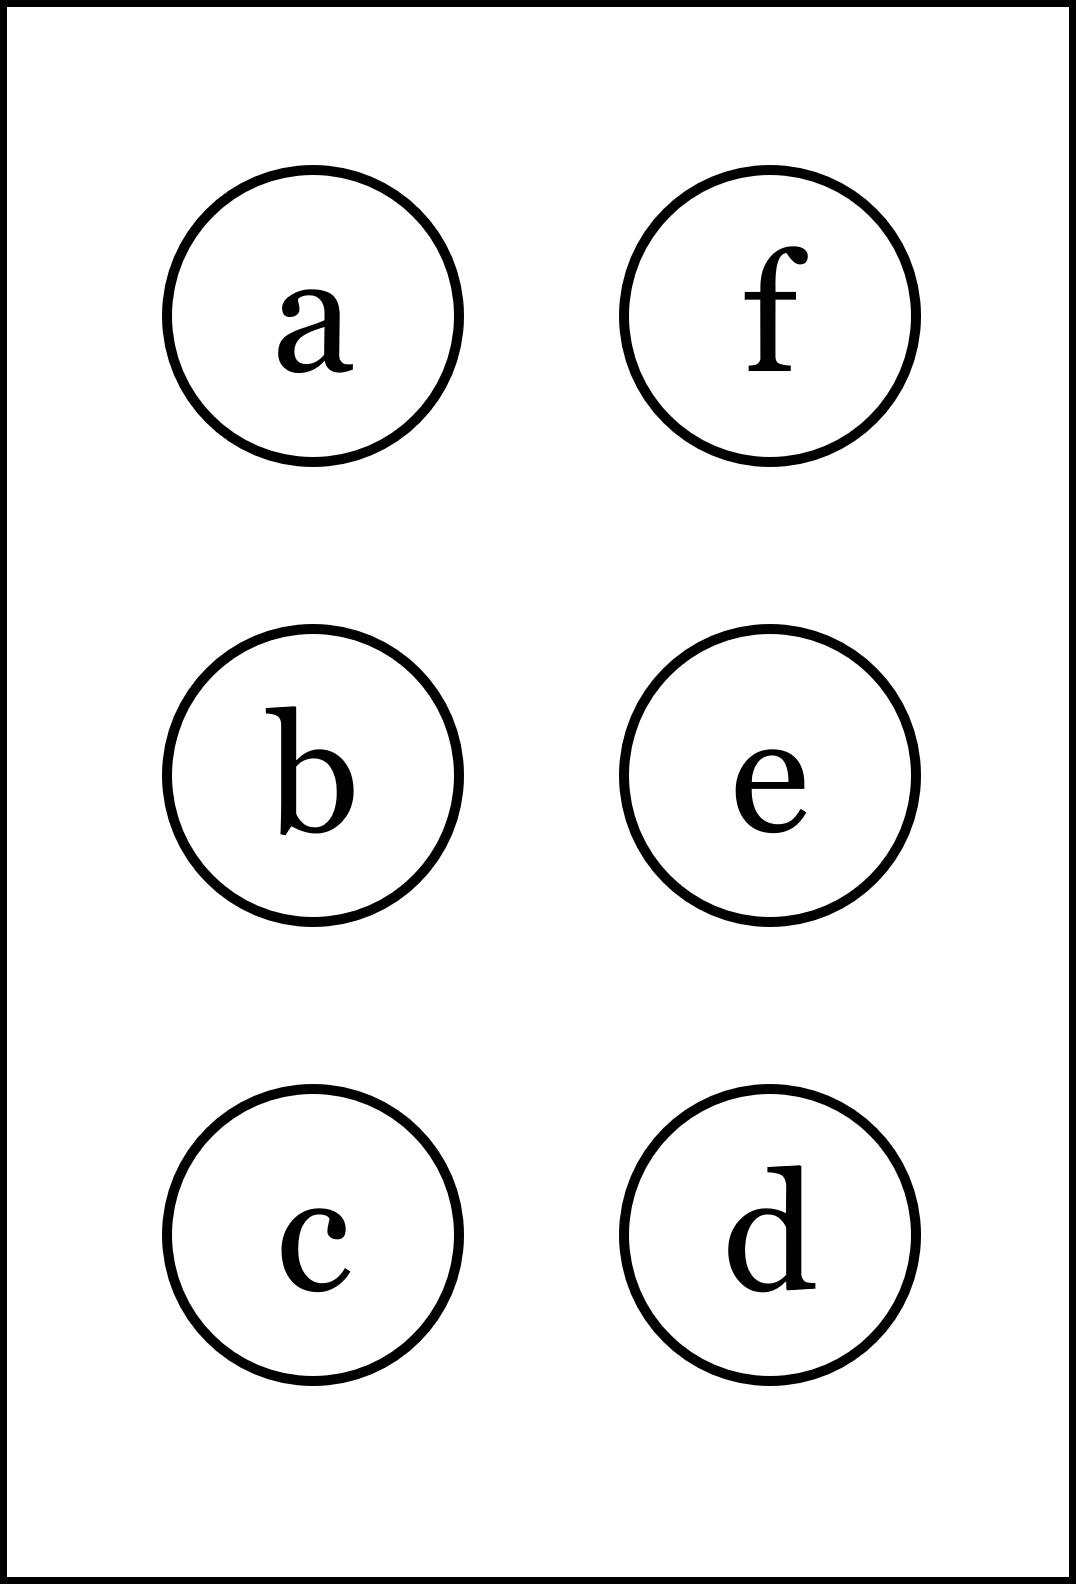
\includegraphics[height=40mm]{../images/braille.png}
{\small Písmeno Braillovej abecedy}
\end{center}
\end{minipage}
\end{center}
\end{minipage}
\\ \hdashline
\begin{minipage}[c][104.5mm][t]{0.5\linewidth}
\begin{center}
\vspace{7mm}
{\huge Volné extrémy, skupina \textit{Epsilon $\epsilon$} -\romannumeral3}\\[5mm]
\textit{Jméno:}\phantom{xxxxxxxxxxxxxxxxxxxxxxxxxxxxxxxxxxxxxxxxxxxxxxxxxxxxxxxxxxxxxxxxx}\\[5mm]
\begin{minipage}{0.95\linewidth}
\begin{center}
Cílem je najít \textbf{volné extrémy} funkce $f(x,y)$ zadané v \textbf{(a)}.\\Postupuj podle krokú v \textbf{(b)} až \textbf{(f)}. Pokud se medzivýsledky shodujú s těmi za otazníky,\\tak napravo obarvi příslušející kroužek načerno. \textbf{Spolu odevzdejte výsledné slovo}.
\end{center}
\end{minipage}
\\[1mm]
\begin{minipage}{0.79\linewidth}
\begin{center}
\begin{varwidth}{\linewidth}
\begin{enumerate}
\normalsize
\item $f(x,y)=2x^3-12x^2-30x-2-108y-18y^2+3y^3$\quad \dotfill\; ???\;\dotfill \quad vybarvi
\item Najdi parciální derivaci podle $x$, $\pdv{f}{x}=$\quad \dotfill\; ???\;\dotfill \quad $6x^2-24x-30$
\item Najdi stacionární body v $x$\quad \dotfill\; ???\;\dotfill \quad $x_1+x_2=5$
\item Najdi parciální derivaci podle $y$, $\pdv{f}{y}=$\quad \dotfill\; ???\;\dotfill \quad $9y^2-36y-72$
\item Najdi stacionární body v $y$\quad \dotfill\; ???\;\dotfill \quad $y_1+y_2=5$
\item Najdi funkční hodnoty vo všech stacionárních bodech \\ \phantom{xxxxxx} a vyber tu najvětší. $f_{\text{max}}(x,y)=$\quad \dotfill\; ???\;\dotfill \quad $-850$
\end{enumerate}
\end{varwidth}
\end{center}
\end{minipage}
\begin{minipage}{0.20\linewidth}
\begin{center}
{\Huge\bfseries 3.} \\[2mm]
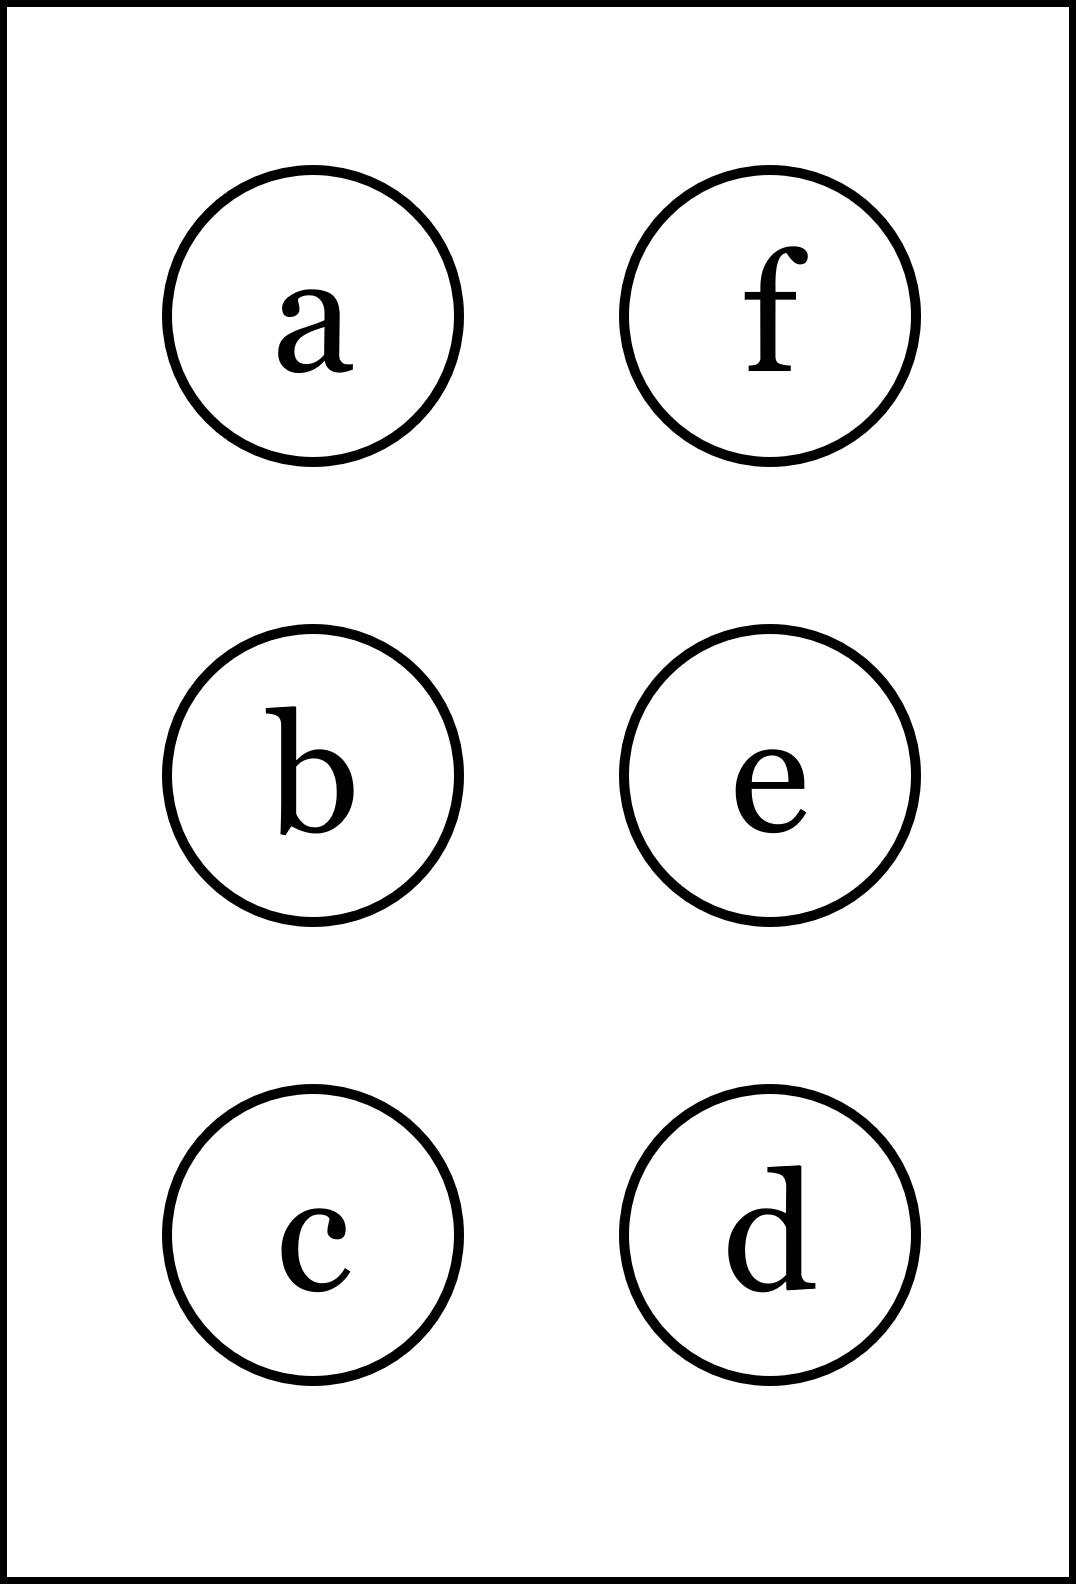
\includegraphics[height=40mm]{../images/braille.png}
{\small Písmeno Braillovej abecedy}
\end{center}
\end{minipage}
\end{center}
\end{minipage}
&
\begin{minipage}[c][104.5mm][t]{0.5\linewidth}
\begin{center}
\vspace{7mm}
{\huge Volné extrémy, skupina \textit{Epsilon $\epsilon$} -\romannumeral4}\\[5mm]
\textit{Jméno:}\phantom{xxxxxxxxxxxxxxxxxxxxxxxxxxxxxxxxxxxxxxxxxxxxxxxxxxxxxxxxxxxxxxxxx}\\[5mm]
\begin{minipage}{0.95\linewidth}
\begin{center}
Cílem je najít \textbf{volné extrémy} funkce $f(x,y)$ zadané v \textbf{(a)}.\\Postupuj podle krokú v \textbf{(b)} až \textbf{(f)}. Pokud se medzivýsledky shodujú s těmi za otazníky,\\tak napravo obarvi příslušející kroužek načerno. \textbf{Spolu odevzdejte výsledné slovo}.
\end{center}
\end{minipage}
\\[1mm]
\begin{minipage}{0.79\linewidth}
\begin{center}
\begin{varwidth}{\linewidth}
\begin{enumerate}
\normalsize
\item $f(x,y)=2x^3-12x^2-30x+3-9y-6y^2-y^3$\quad \dotfill\; ???\;\dotfill \quad vybarvi
\item Najdi parciální derivaci podle $x$, $\pdv{f}{x}=$\quad \dotfill\; ???\;\dotfill \quad $6x^2-12x-30$
\item Najdi stacionární body v $x$\quad \dotfill\; ???\;\dotfill \quad $x_1+x_2=5$
\item Najdi parciální derivaci podle $y$, $\pdv{f}{y}=$\quad \dotfill\; ???\;\dotfill \quad $-3y^2-12y-3$
\item Najdi stacionární body v $y$\quad \dotfill\; ???\;\dotfill \quad $y_1+y_2=-3$
\item Najdi funkční hodnoty vo všech stacionárních bodech \\ \phantom{xxxxxx} a vyber tu najvětší. $f_{\text{max}}(x,y)=$\quad \dotfill\; ???\;\dotfill \quad $-197$
\end{enumerate}
\end{varwidth}
\end{center}
\end{minipage}
\begin{minipage}{0.20\linewidth}
\begin{center}
{\Huge\bfseries 4.} \\[2mm]
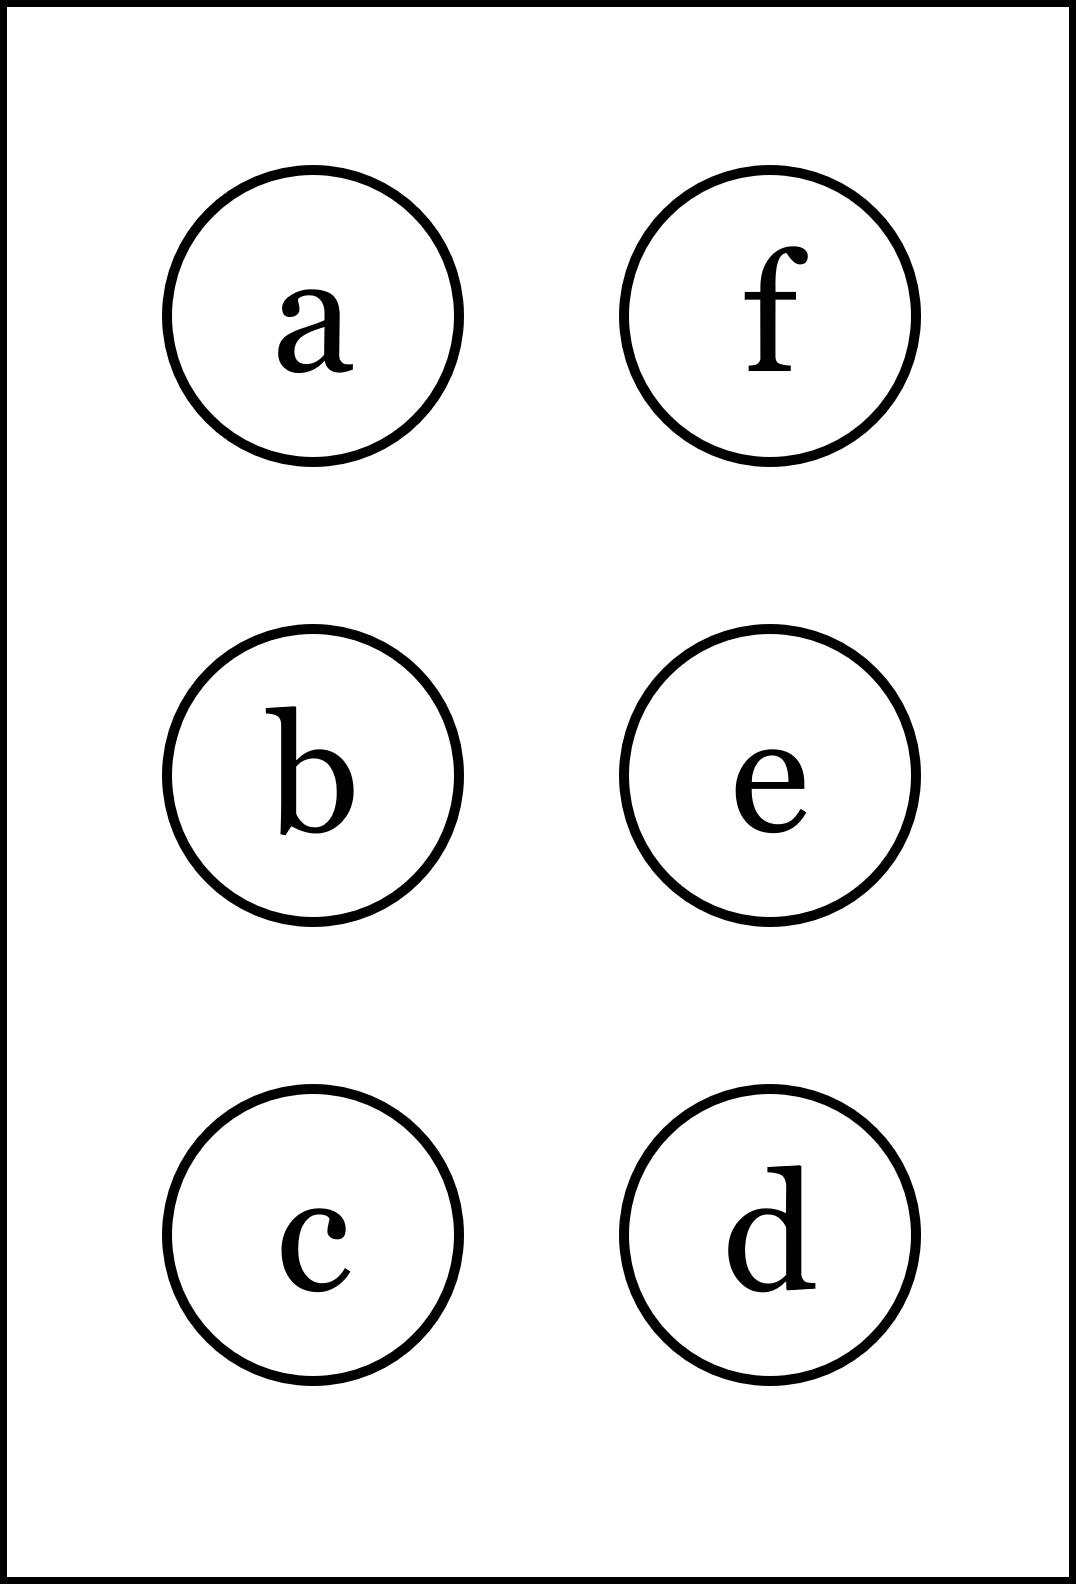
\includegraphics[height=40mm]{../images/braille.png}
{\small Písmeno Braillovej abecedy}
\end{center}
\end{minipage}
\end{center}
\end{minipage}
%
\end{tabular}
\newpage
\thispagestyle{empty}
\begin{tabular}{c:c}
\begin{minipage}[c][104.5mm][t]{0.5\linewidth}
\begin{center}
\vspace{7mm}
{\huge Volné extrémy, skupina \textit{Zeta $\zeta$} -\romannumeral1}\\[5mm]
\textit{Jméno:}\phantom{xxxxxxxxxxxxxxxxxxxxxxxxxxxxxxxxxxxxxxxxxxxxxxxxxxxxxxxxxxxxxxxxx}\\[5mm]
\begin{minipage}{0.95\linewidth}
\begin{center}
Cílem je najít \textbf{volné extrémy} funkce $f(x,y)$ zadané v \textbf{(a)}.\\Postupuj podle krokú v \textbf{(b)} až \textbf{(f)}. Pokud se medzivýsledky shodujú s těmi za otazníky,\\tak napravo obarvi příslušející kroužek načerno. \textbf{Spolu odevzdejte výsledné slovo}.
\end{center}
\end{minipage}
\\[1mm]
\begin{minipage}{0.79\linewidth}
\begin{center}
\begin{varwidth}{\linewidth}
\begin{enumerate}
\normalsize
\item $f(x,y)=-3x^3+18x^2+108x-2+48y+6y^2-2y^3$\quad \dotfill\; ???\;\dotfill \quad vybarvi
\item Najdi parciální derivaci podle $x$, $\pdv{f}{x}=$\quad \dotfill\; ???\;\dotfill \quad $-9x^2+36x+108$
\item Najdi stacionární body v $x$\quad \dotfill\; ???\;\dotfill \quad $x_1+x_2=5$
\item Najdi parciální derivaci podle $y$, $\pdv{f}{y}=$\quad \dotfill\; ???\;\dotfill \quad $-6y^2+12y+36$
\item Najdi stacionární body v $y$\quad \dotfill\; ???\;\dotfill \quad $y_1+y_2=2$
\item Najdi funkční hodnoty vo všech stacionárních bodech \\ \phantom{xxxxxx} a vyber tu najvětší. $f_{\text{max}}(x,y)=$\quad \dotfill\; ???\;\dotfill \quad $590$
\end{enumerate}
\end{varwidth}
\end{center}
\end{minipage}
\begin{minipage}{0.20\linewidth}
\begin{center}
{\Huge\bfseries 1.} \\[2mm]
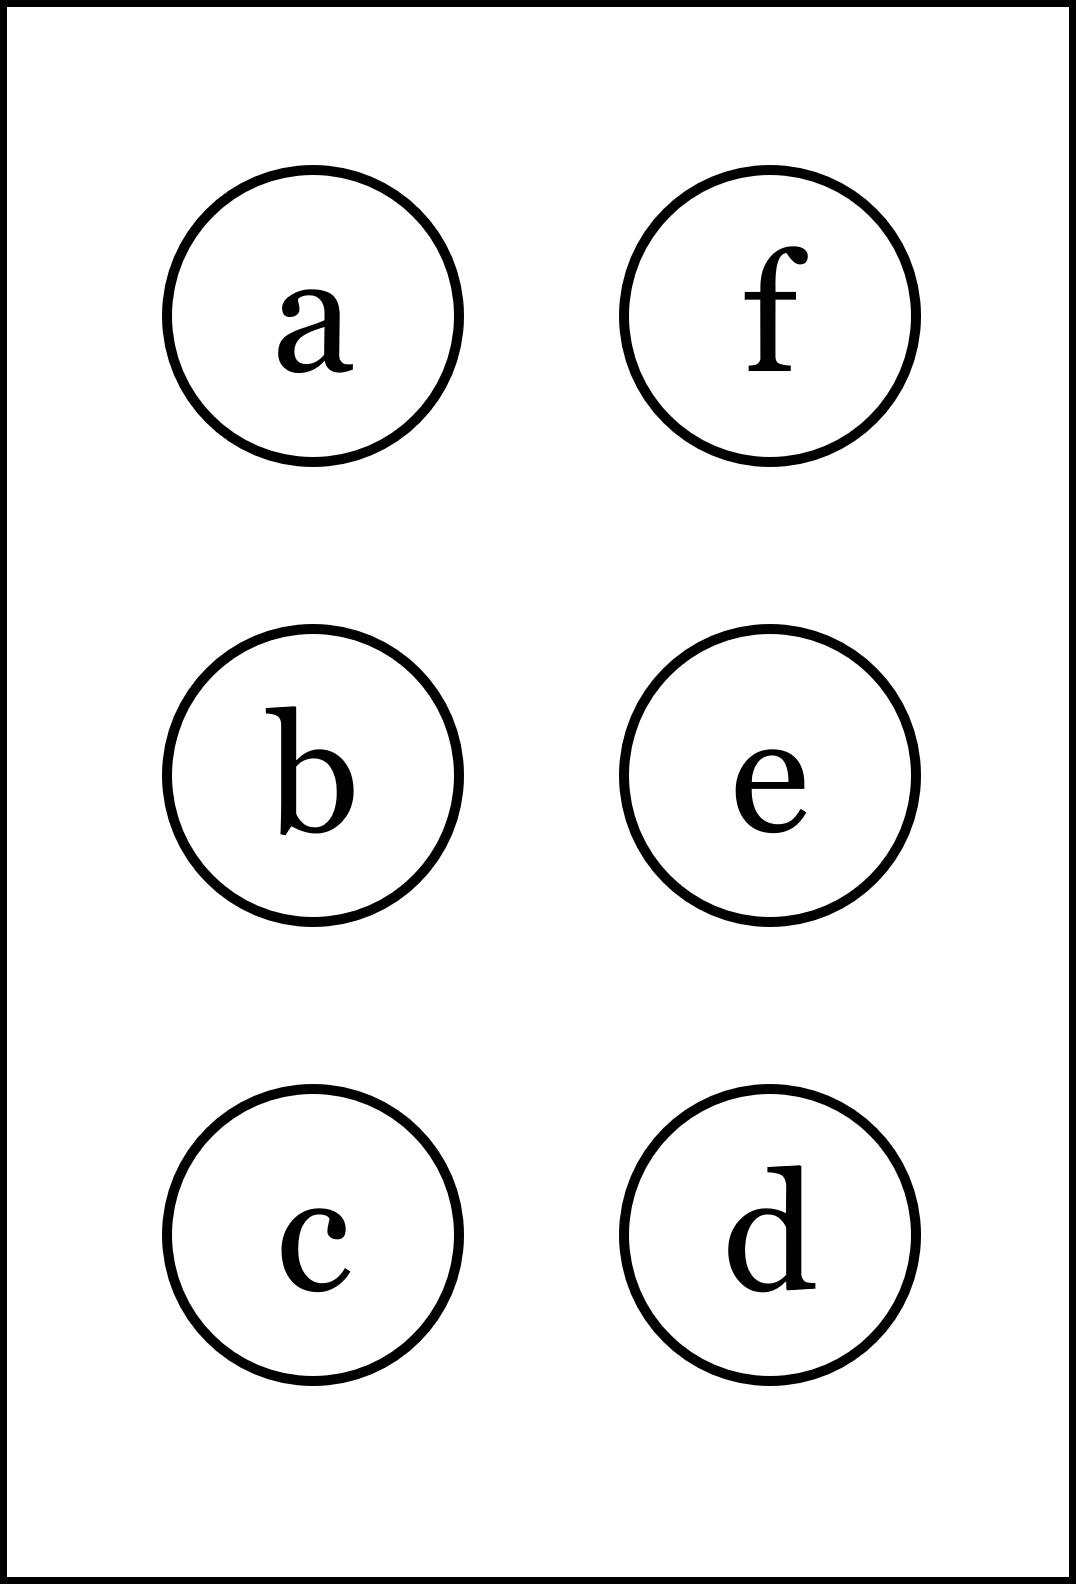
\includegraphics[height=40mm]{../images/braille.png}
{\small Písmeno Braillovej abecedy}
\end{center}
\end{minipage}
\end{center}
\end{minipage}
&
\begin{minipage}[c][104.5mm][t]{0.5\linewidth}
\begin{center}
\vspace{7mm}
{\huge Volné extrémy, skupina \textit{Zeta $\zeta$} -\romannumeral2}\\[5mm]
\textit{Jméno:}\phantom{xxxxxxxxxxxxxxxxxxxxxxxxxxxxxxxxxxxxxxxxxxxxxxxxxxxxxxxxxxxxxxxxx}\\[5mm]
\begin{minipage}{0.95\linewidth}
\begin{center}
Cílem je najít \textbf{volné extrémy} funkce $f(x,y)$ zadané v \textbf{(a)}.\\Postupuj podle krokú v \textbf{(b)} až \textbf{(f)}. Pokud se medzivýsledky shodujú s těmi za otazníky,\\tak napravo obarvi příslušející kroužek načerno. \textbf{Spolu odevzdejte výsledné slovo}.
\end{center}
\end{minipage}
\\[1mm]
\begin{minipage}{0.79\linewidth}
\begin{center}
\begin{varwidth}{\linewidth}
\begin{enumerate}
\normalsize
\item $f(x,y)=-3x^3-18x^2+45x-5+144y-18y^2-6y^3$\quad \dotfill\; ???\;\dotfill \quad vybarvi
\item Najdi parciální derivaci podle $x$, $\pdv{f}{x}=$\quad \dotfill\; ???\;\dotfill \quad $-9x^2-18x+45$
\item Najdi stacionární body v $x$\quad \dotfill\; ???\;\dotfill \quad $x_1+x_2=-4$
\item Najdi parciální derivaci podle $y$, $\pdv{f}{y}=$\quad \dotfill\; ???\;\dotfill \quad $-18y^2-36y+108$
\item Najdi stacionární body v $y$\quad \dotfill\; ???\;\dotfill \quad $y_1+y_2=-2$
\item Najdi funkční hodnoty vo všech stacionárních bodech \\ \phantom{xxxxxx} a vyber tu najvětší. $f_{\text{max}}(x,y)=$\quad \dotfill\; ???\;\dotfill \quad $-785$
\end{enumerate}
\end{varwidth}
\end{center}
\end{minipage}
\begin{minipage}{0.20\linewidth}
\begin{center}
{\Huge\bfseries 2.} \\[2mm]
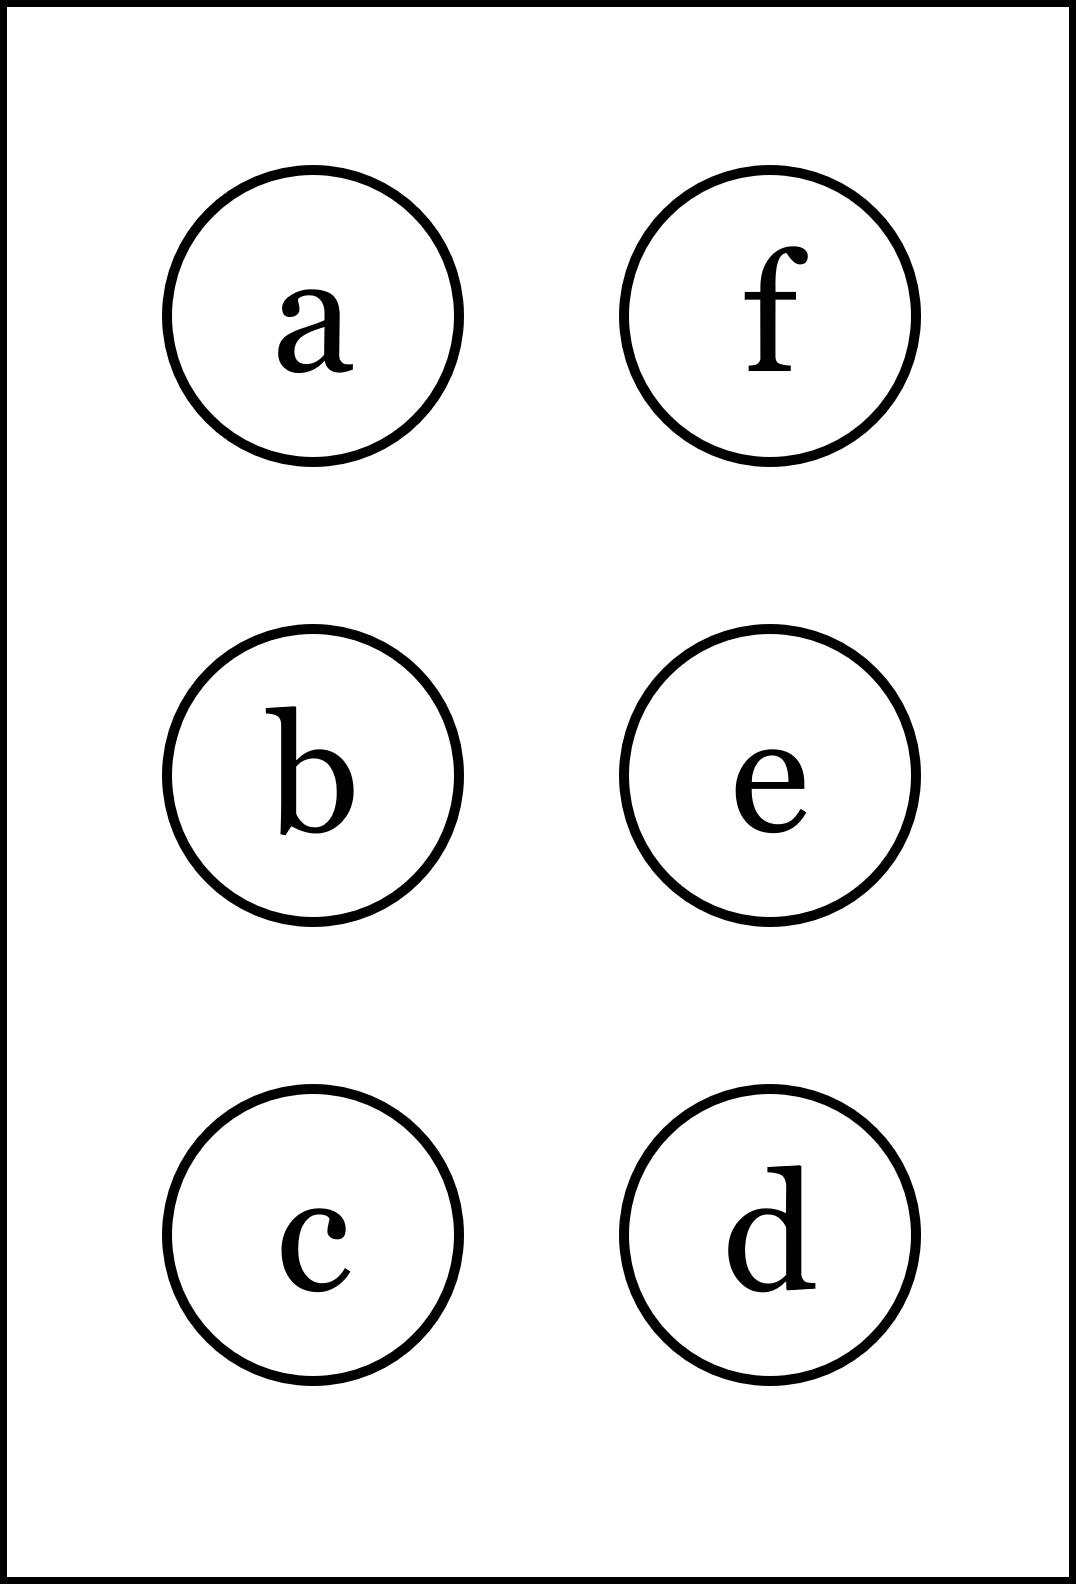
\includegraphics[height=40mm]{../images/braille.png}
{\small Písmeno Braillovej abecedy}
\end{center}
\end{minipage}
\end{center}
\end{minipage}
\\ \hdashline
\begin{minipage}[c][104.5mm][t]{0.5\linewidth}
\begin{center}
\vspace{7mm}
{\huge Volné extrémy, skupina \textit{Zeta $\zeta$} -\romannumeral3}\\[5mm]
\textit{Jméno:}\phantom{xxxxxxxxxxxxxxxxxxxxxxxxxxxxxxxxxxxxxxxxxxxxxxxxxxxxxxxxxxxxxxxxx}\\[5mm]
\begin{minipage}{0.95\linewidth}
\begin{center}
Cílem je najít \textbf{volné extrémy} funkce $f(x,y)$ zadané v \textbf{(a)}.\\Postupuj podle krokú v \textbf{(b)} až \textbf{(f)}. Pokud se medzivýsledky shodujú s těmi za otazníky,\\tak napravo obarvi příslušející kroužek načerno. \textbf{Spolu odevzdejte výsledné slovo}.
\end{center}
\end{minipage}
\\[1mm]
\begin{minipage}{0.79\linewidth}
\begin{center}
\begin{varwidth}{\linewidth}
\begin{enumerate}
\normalsize
\item $f(x,y)=-6x^3-36x^2-54x+6+9y+6y^2+y^3$\quad \dotfill\; ???\;\dotfill \quad vybarvi
\item Najdi parciální derivaci podle $x$, $\pdv{f}{x}=$\quad \dotfill\; ???\;\dotfill \quad $-18x^2-72x-54$
\item Najdi stacionární body v $x$\quad \dotfill\; ???\;\dotfill \quad $x_1+x_2=-4$
\item Najdi parciální derivaci podle $y$, $\pdv{f}{y}=$\quad \dotfill\; ???\;\dotfill \quad $3y^2+12y-9$
\item Najdi stacionární body v $y$\quad \dotfill\; ???\;\dotfill \quad $y_1+y_2=-4$
\item Najdi funkční hodnoty vo všech stacionárních bodech \\ \phantom{xxxxxx} a vyber tu najvětší. $f_{\text{max}}(x,y)=$\quad \dotfill\; ???\;\dotfill \quad $2$
\end{enumerate}
\end{varwidth}
\end{center}
\end{minipage}
\begin{minipage}{0.20\linewidth}
\begin{center}
{\Huge\bfseries 3.} \\[2mm]
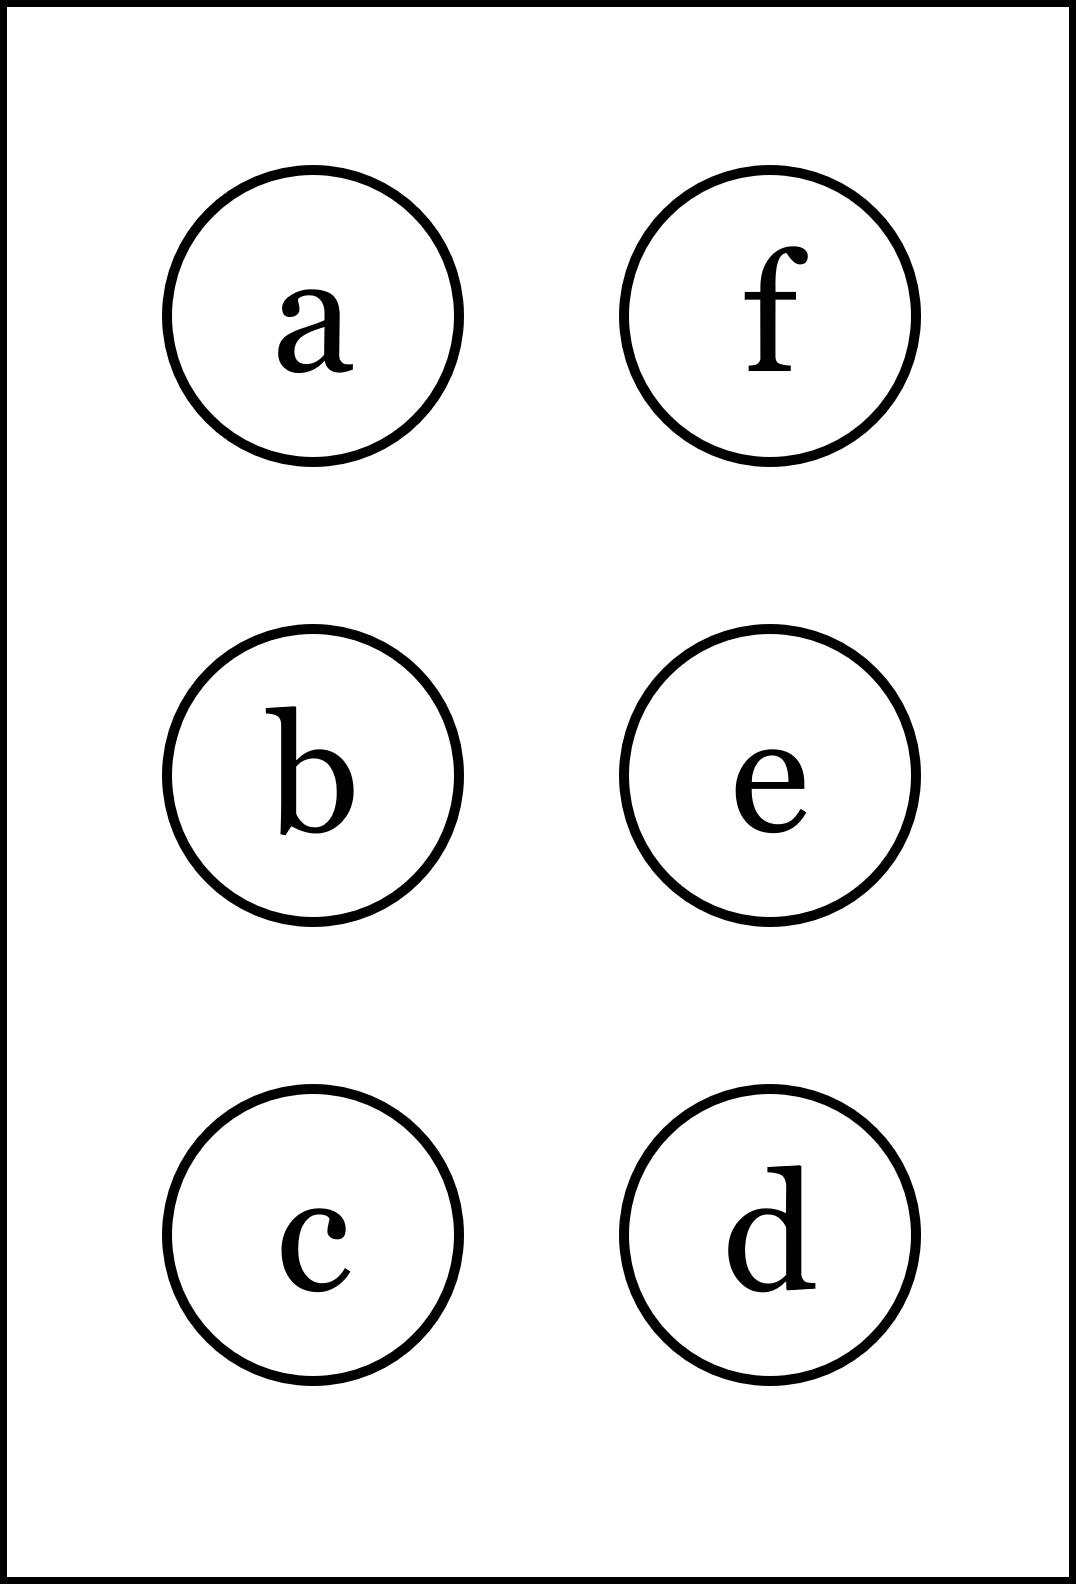
\includegraphics[height=40mm]{../images/braille.png}
{\small Písmeno Braillovej abecedy}
\end{center}
\end{minipage}
\end{center}
\end{minipage}
&
\begin{minipage}[c][104.5mm][t]{0.5\linewidth}
\begin{center}
\vspace{7mm}
{\huge Volné extrémy, skupina \textit{Zeta $\zeta$} -\romannumeral4}\\[5mm]
\textit{Jméno:}\phantom{xxxxxxxxxxxxxxxxxxxxxxxxxxxxxxxxxxxxxxxxxxxxxxxxxxxxxxxxxxxxxxxxx}\\[5mm]
\begin{minipage}{0.95\linewidth}
\begin{center}
Cílem je najít \textbf{volné extrémy} funkce $f(x,y)$ zadané v \textbf{(a)}.\\Postupuj podle krokú v \textbf{(b)} až \textbf{(f)}. Pokud se medzivýsledky shodujú s těmi za otazníky,\\tak napravo obarvi příslušející kroužek načerno. \textbf{Spolu odevzdejte výsledné slovo}.
\end{center}
\end{minipage}
\\[1mm]
\begin{minipage}{0.79\linewidth}
\begin{center}
\begin{varwidth}{\linewidth}
\begin{enumerate}
\normalsize
\item $f(x,y)=4x^3+12x^2-96x-3+63y-6y^2-y^3$\quad \dotfill\; ???\;\dotfill \quad vybarvi
\item Najdi parciální derivaci podle $x$, $\pdv{f}{x}=$\quad \dotfill\; ???\;\dotfill \quad $12x^2+12x-96$
\item Najdi stacionární body v $x$\quad \dotfill\; ???\;\dotfill \quad $x_1+x_2=-1$
\item Najdi parciální derivaci podle $y$, $\pdv{f}{y}=$\quad \dotfill\; ???\;\dotfill \quad $-3y^2-12y+45$
\item Najdi stacionární body v $y$\quad \dotfill\; ???\;\dotfill \quad $y_1+y_2=-3$
\item Najdi funkční hodnoty vo všech stacionárních bodech \\ \phantom{xxxxxx} a vyber tu najvětší. $f_{\text{max}}(x,y)=$\quad \dotfill\; ???\;\dotfill \quad $-507$
\end{enumerate}
\end{varwidth}
\end{center}
\end{minipage}
\begin{minipage}{0.20\linewidth}
\begin{center}
{\Huge\bfseries 4.} \\[2mm]
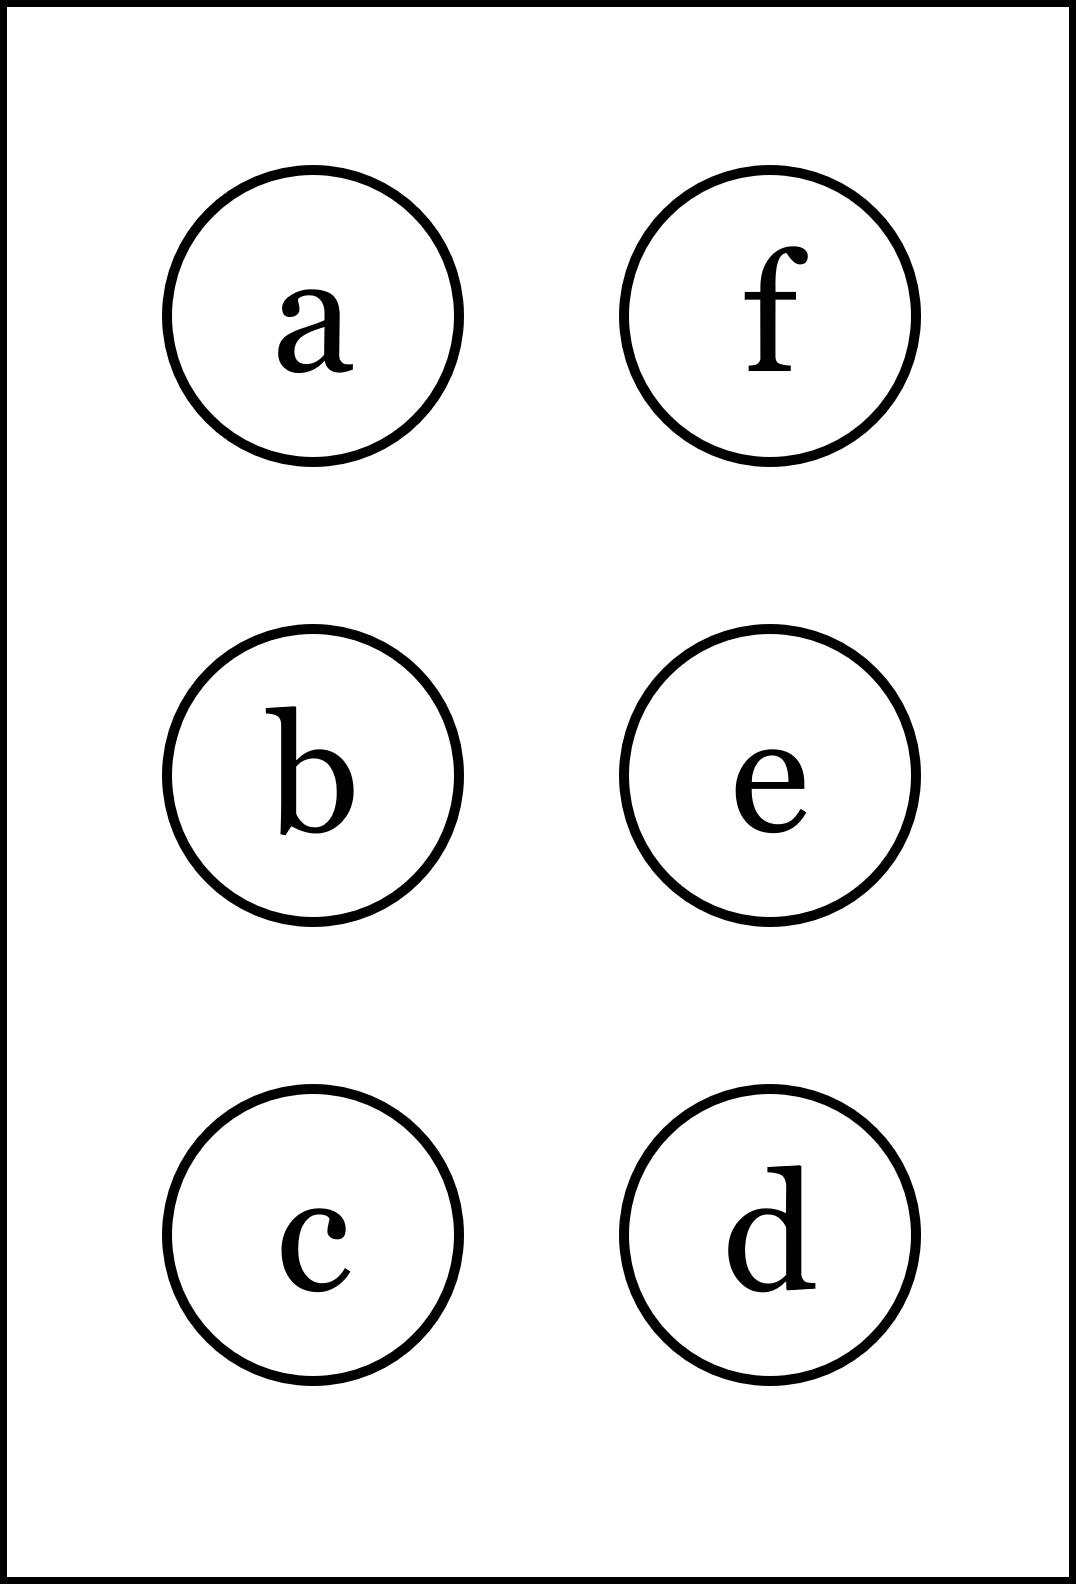
\includegraphics[height=40mm]{../images/braille.png}
{\small Písmeno Braillovej abecedy}
\end{center}
\end{minipage}
\end{center}
\end{minipage}
%
\end{tabular}
\newpage
\thispagestyle{empty}
\begin{tabular}{c:c}
\begin{minipage}[c][104.5mm][t]{0.5\linewidth}
\begin{center}
\vspace{7mm}
{\huge Volné extrémy, skupina \textit{Eta $\eta$} -\romannumeral1}\\[5mm]
\textit{Jméno:}\phantom{xxxxxxxxxxxxxxxxxxxxxxxxxxxxxxxxxxxxxxxxxxxxxxxxxxxxxxxxxxxxxxxxx}\\[5mm]
\begin{minipage}{0.95\linewidth}
\begin{center}
Cílem je najít \textbf{volné extrémy} funkce $f(x,y)$ zadané v \textbf{(a)}.\\Postupuj podle krokú v \textbf{(b)} až \textbf{(f)}. Pokud se medzivýsledky shodujú s těmi za otazníky,\\tak napravo obarvi příslušející kroužek načerno. \textbf{Spolu odevzdejte výsledné slovo}.
\end{center}
\end{minipage}
\\[1mm]
\begin{minipage}{0.79\linewidth}
\begin{center}
\begin{varwidth}{\linewidth}
\begin{enumerate}
\normalsize
\item $f(x,y)=3x^3-18x^2-45x-2+45y-18y^2-3y^3$\quad \dotfill\; ???\;\dotfill \quad vybarvi
\item Najdi parciální derivaci podle $x$, $\pdv{f}{x}=$\quad \dotfill\; ???\;\dotfill \quad $9x^2-18x-45$
\item Najdi stacionární body v $x$\quad \dotfill\; ???\;\dotfill \quad $x_1+x_2=4$
\item Najdi parciální derivaci podle $y$, $\pdv{f}{y}=$\quad \dotfill\; ???\;\dotfill \quad $-9y^2-36y+45$
\item Najdi stacionární body v $y$\quad \dotfill\; ???\;\dotfill \quad $y_1+y_2=-3$
\item Najdi funkční hodnoty vo všech stacionárních bodech \\ \phantom{xxxxxx} a vyber tu najvětší. $f_{\text{max}}(x,y)=$\quad \dotfill\; ???\;\dotfill \quad $-602$
\end{enumerate}
\end{varwidth}
\end{center}
\end{minipage}
\begin{minipage}{0.20\linewidth}
\begin{center}
{\Huge\bfseries 1.} \\[2mm]
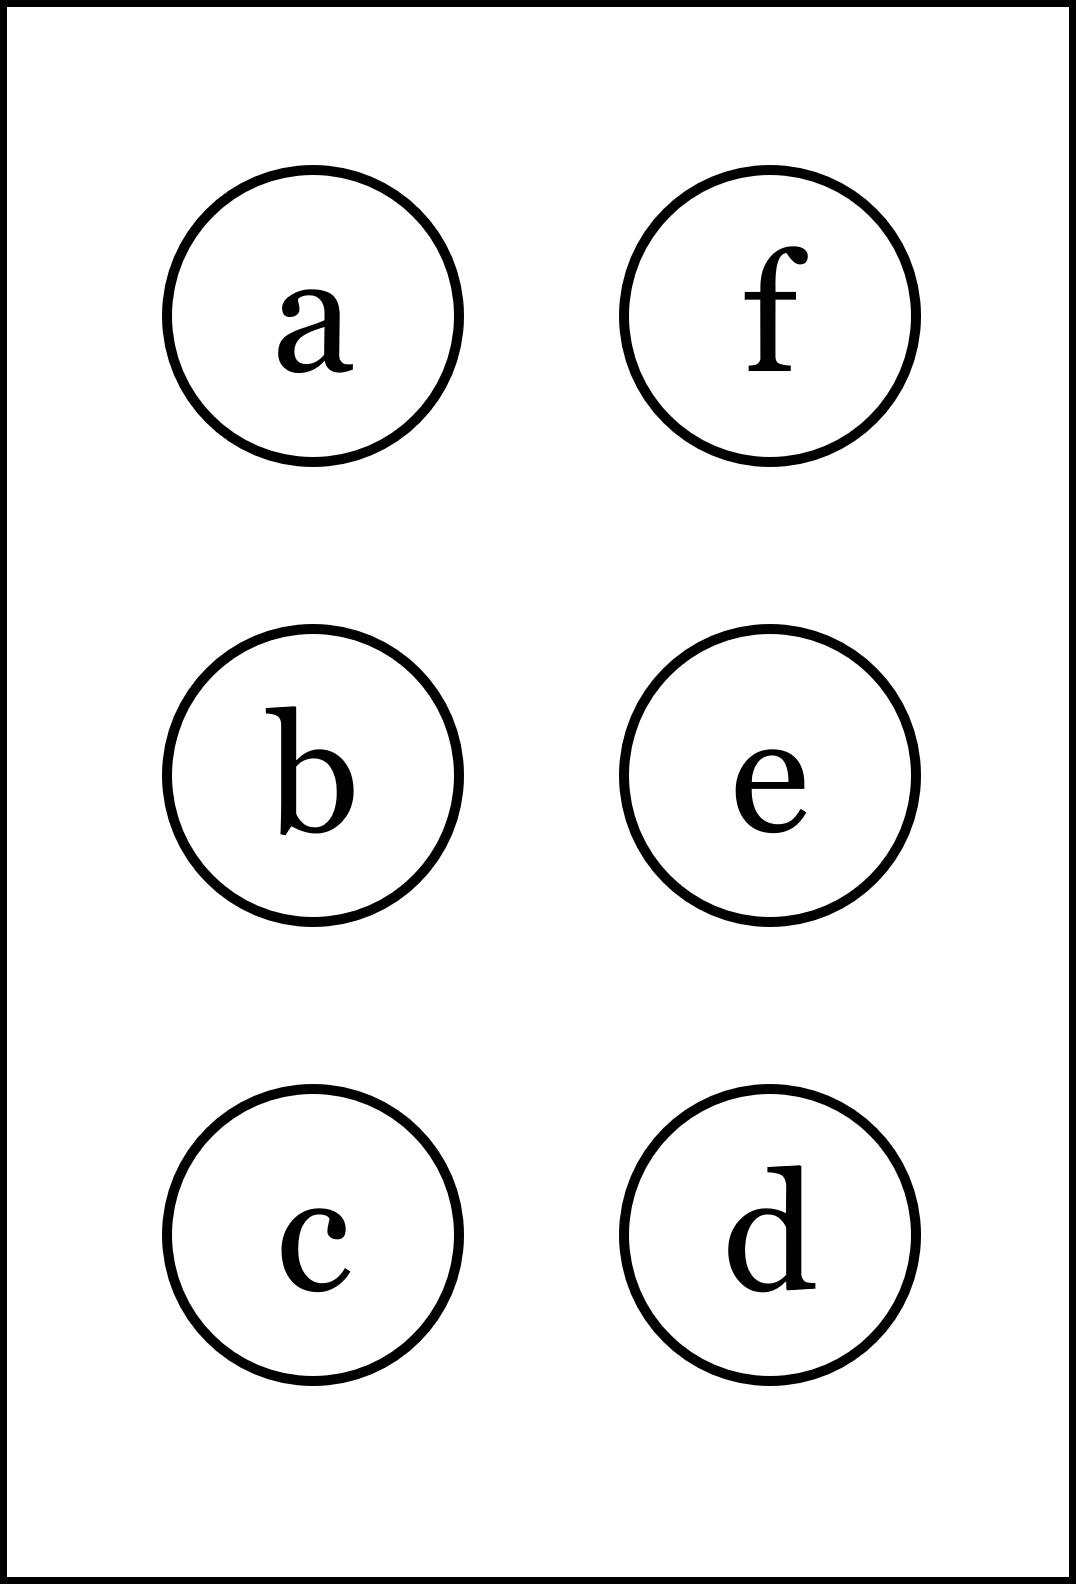
\includegraphics[height=40mm]{../images/braille.png}
{\small Písmeno Braillovej abecedy}
\end{center}
\end{minipage}
\end{center}
\end{minipage}
&
\begin{minipage}[c][104.5mm][t]{0.5\linewidth}
\begin{center}
\vspace{7mm}
{\huge Volné extrémy, skupina \textit{Eta $\eta$} -\romannumeral2}\\[5mm]
\textit{Jméno:}\phantom{xxxxxxxxxxxxxxxxxxxxxxxxxxxxxxxxxxxxxxxxxxxxxxxxxxxxxxxxxxxxxxxxx}\\[5mm]
\begin{minipage}{0.95\linewidth}
\begin{center}
Cílem je najít \textbf{volné extrémy} funkce $f(x,y)$ zadané v \textbf{(a)}.\\Postupuj podle krokú v \textbf{(b)} až \textbf{(f)}. Pokud se medzivýsledky shodujú s těmi za otazníky,\\tak napravo obarvi příslušející kroužek načerno. \textbf{Spolu odevzdejte výsledné slovo}.
\end{center}
\end{minipage}
\\[1mm]
\begin{minipage}{0.79\linewidth}
\begin{center}
\begin{varwidth}{\linewidth}
\begin{enumerate}
\normalsize
\item $f(x,y)=-4x^3-12x^2+96x-1-9y+6y^2-y^3$\quad \dotfill\; ???\;\dotfill \quad vybarvi
\item Najdi parciální derivaci podle $x$, $\pdv{f}{x}=$\quad \dotfill\; ???\;\dotfill \quad $-12x^2-24x+96$
\item Najdi stacionární body v $x$\quad \dotfill\; ???\;\dotfill \quad $x_1+x_2=-2$
\item Najdi parciální derivaci podle $y$, $\pdv{f}{y}=$\quad \dotfill\; ???\;\dotfill \quad $-3y^2+12y-3$
\item Najdi stacionární body v $y$\quad \dotfill\; ???\;\dotfill \quad $y_1+y_2=4$
\item Najdi funkční hodnoty vo všech stacionárních bodech \\ \phantom{xxxxxx} a vyber tu najvětší. $f_{\text{max}}(x,y)=$\quad \dotfill\; ???\;\dotfill \quad $107$
\end{enumerate}
\end{varwidth}
\end{center}
\end{minipage}
\begin{minipage}{0.20\linewidth}
\begin{center}
{\Huge\bfseries 2.} \\[2mm]
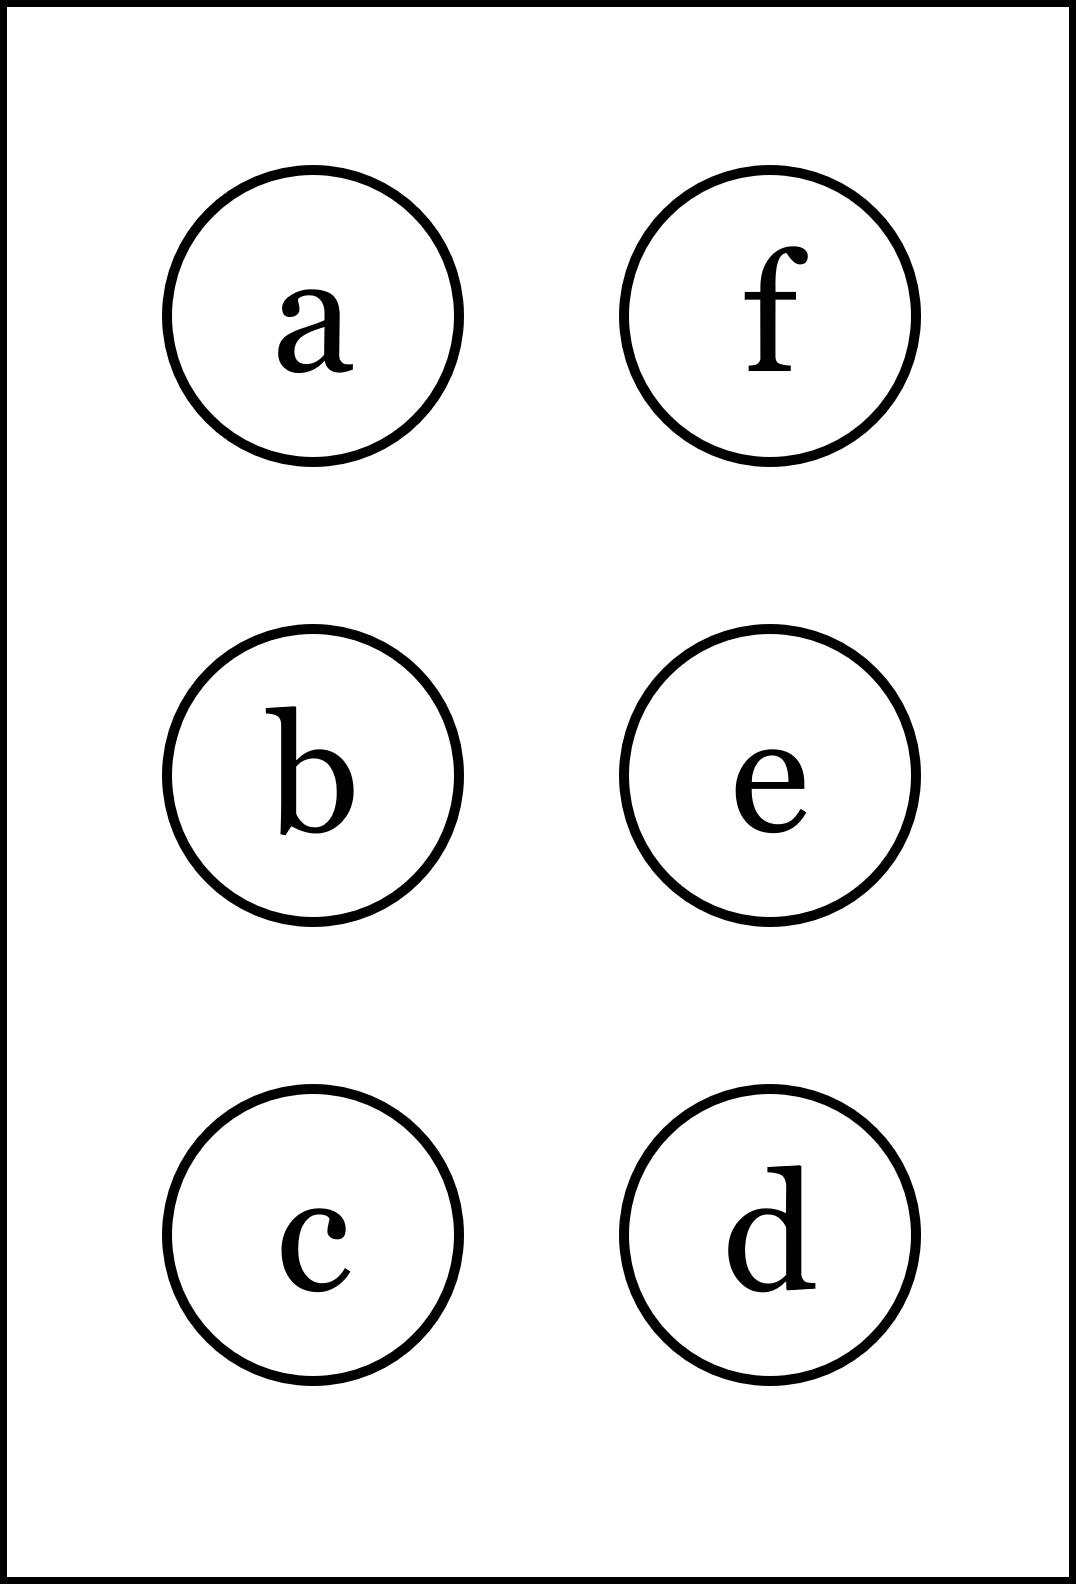
\includegraphics[height=40mm]{../images/braille.png}
{\small Písmeno Braillovej abecedy}
\end{center}
\end{minipage}
\end{center}
\end{minipage}
\\ \hdashline
\begin{minipage}[c][104.5mm][t]{0.5\linewidth}
\begin{center}
\vspace{7mm}
{\huge Volné extrémy, skupina \textit{Eta $\eta$} -\romannumeral3}\\[5mm]
\textit{Jméno:}\phantom{xxxxxxxxxxxxxxxxxxxxxxxxxxxxxxxxxxxxxxxxxxxxxxxxxxxxxxxxxxxxxxxxx}\\[5mm]
\begin{minipage}{0.95\linewidth}
\begin{center}
Cílem je najít \textbf{volné extrémy} funkce $f(x,y)$ zadané v \textbf{(a)}.\\Postupuj podle krokú v \textbf{(b)} až \textbf{(f)}. Pokud se medzivýsledky shodujú s těmi za otazníky,\\tak napravo obarvi příslušející kroužek načerno. \textbf{Spolu odevzdejte výsledné slovo}.
\end{center}
\end{minipage}
\\[1mm]
\begin{minipage}{0.79\linewidth}
\begin{center}
\begin{varwidth}{\linewidth}
\begin{enumerate}
\normalsize
\item $f(x,y)=-x^3+6x^2-9x+7+216y-36y^2-6y^3$\quad \dotfill\; ???\;\dotfill \quad vybarvi
\item Najdi parciální derivaci podle $x$, $\pdv{f}{x}=$\quad \dotfill\; ???\;\dotfill \quad $-3x^2+6x-9$
\item Najdi stacionární body v $x$\quad \dotfill\; ???\;\dotfill \quad $x_1+x_2=4$
\item Najdi parciální derivaci podle $y$, $\pdv{f}{y}=$\quad \dotfill\; ???\;\dotfill \quad $-18y^2-72y+144$
\item Najdi stacionární body v $y$\quad \dotfill\; ???\;\dotfill \quad $y_1+y_2=-4$
\item Najdi funkční hodnoty vo všech stacionárních bodech \\ \phantom{xxxxxx} a vyber tu najvětší. $f_{\text{max}}(x,y)=$\quad \dotfill\; ???\;\dotfill \quad $247$
\end{enumerate}
\end{varwidth}
\end{center}
\end{minipage}
\begin{minipage}{0.20\linewidth}
\begin{center}
{\Huge\bfseries 3.} \\[2mm]
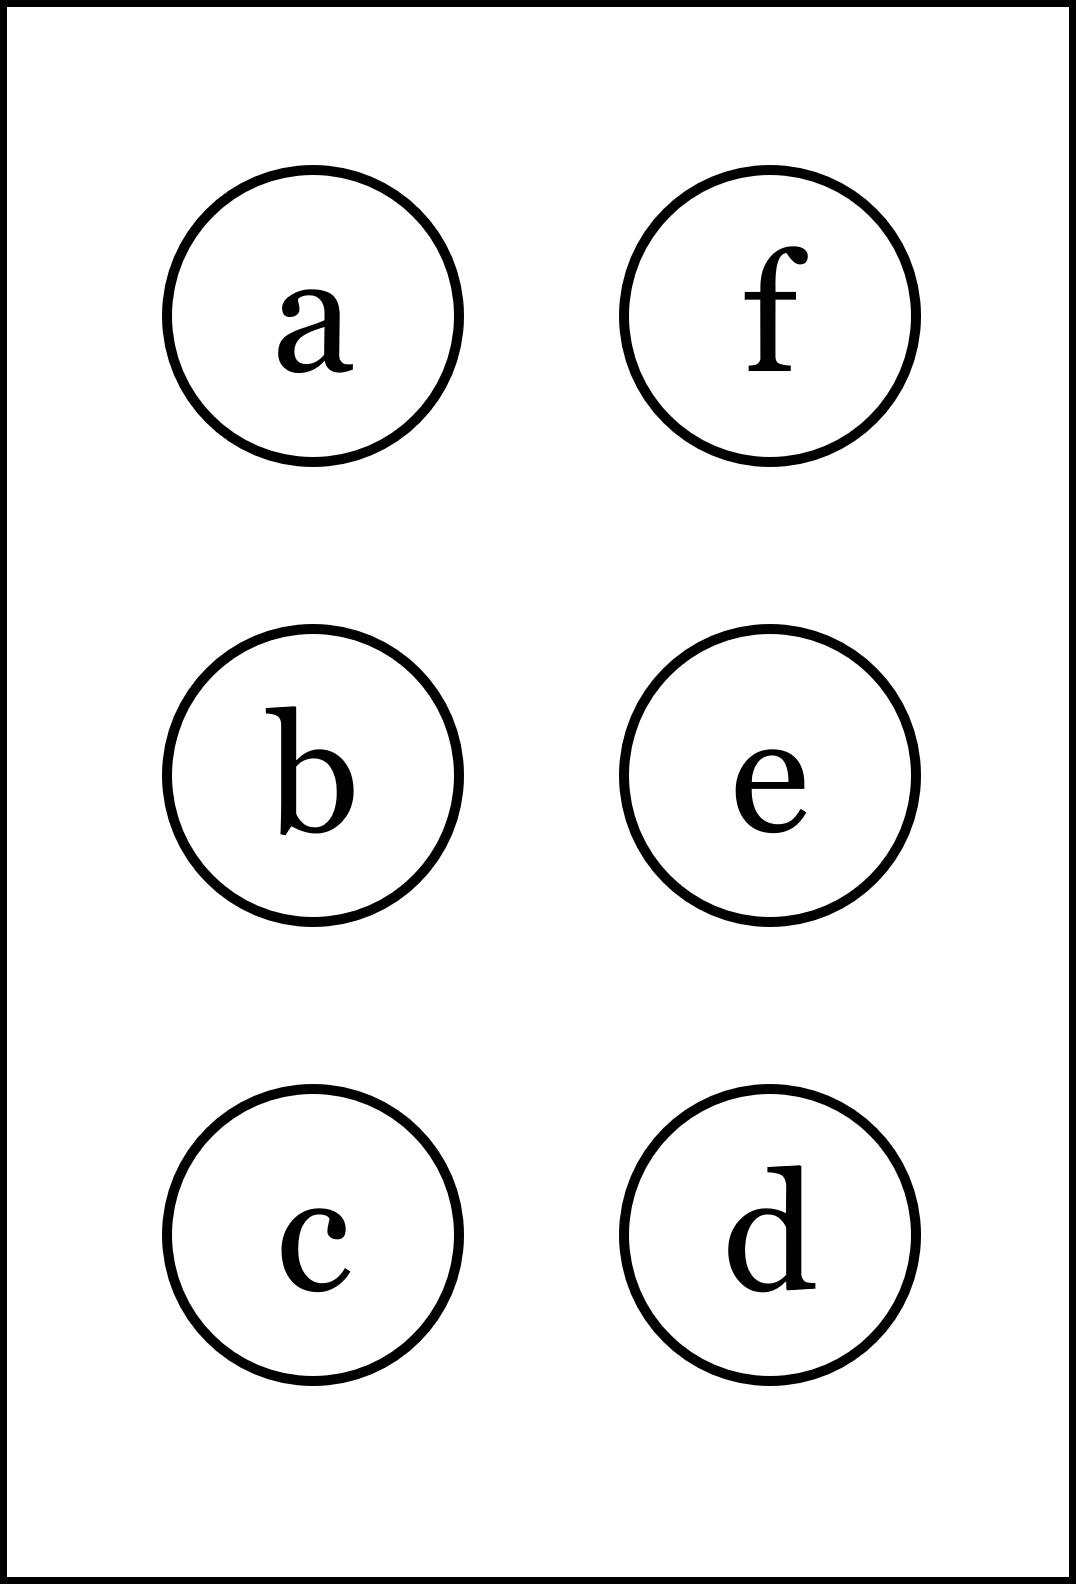
\includegraphics[height=40mm]{../images/braille.png}
{\small Písmeno Braillovej abecedy}
\end{center}
\end{minipage}
\end{center}
\end{minipage}
&
\begin{minipage}[c][104.5mm][t]{0.5\linewidth}
\begin{center}
\vspace{7mm}
{\huge Volné extrémy, skupina \textit{Eta $\eta$} -\romannumeral4}\\[5mm]
\textit{Jméno:}\phantom{xxxxxxxxxxxxxxxxxxxxxxxxxxxxxxxxxxxxxxxxxxxxxxxxxxxxxxxxxxxxxxxxx}\\[5mm]
\begin{minipage}{0.95\linewidth}
\begin{center}
Cílem je najít \textbf{volné extrémy} funkce $f(x,y)$ zadané v \textbf{(a)}.\\Postupuj podle krokú v \textbf{(b)} až \textbf{(f)}. Pokud se medzivýsledky shodujú s těmi za otazníky,\\tak napravo obarvi příslušející kroužek načerno. \textbf{Spolu odevzdejte výsledné slovo}.
\end{center}
\end{minipage}
\\[1mm]
\begin{minipage}{0.79\linewidth}
\begin{center}
\begin{varwidth}{\linewidth}
\begin{enumerate}
\normalsize
\item $f(x,y)=-x^3-6x^2+15x-1-9y-3y^2+y^3$\quad \dotfill\; ???\;\dotfill \quad vybarvi
\item Najdi parciální derivaci podle $x$, $\pdv{f}{x}=$\quad \dotfill\; ???\;\dotfill \quad $-3x^2-6x+15$
\item Najdi stacionární body v $x$\quad \dotfill\; ???\;\dotfill \quad $x_1+x_2=-3$
\item Najdi parciální derivaci podle $y$, $\pdv{f}{y}=$\quad \dotfill\; ???\;\dotfill \quad $3y^2-6y-6$
\item Najdi stacionární body v $y$\quad \dotfill\; ???\;\dotfill \quad $y_1+y_2=3$
\item Najdi funkční hodnoty vo všech stacionárních bodech \\ \phantom{xxxxxx} a vyber tu najvětší. $f_{\text{max}}(x,y)=$\quad \dotfill\; ???\;\dotfill \quad $-128$
\end{enumerate}
\end{varwidth}
\end{center}
\end{minipage}
\begin{minipage}{0.20\linewidth}
\begin{center}
{\Huge\bfseries 4.} \\[2mm]
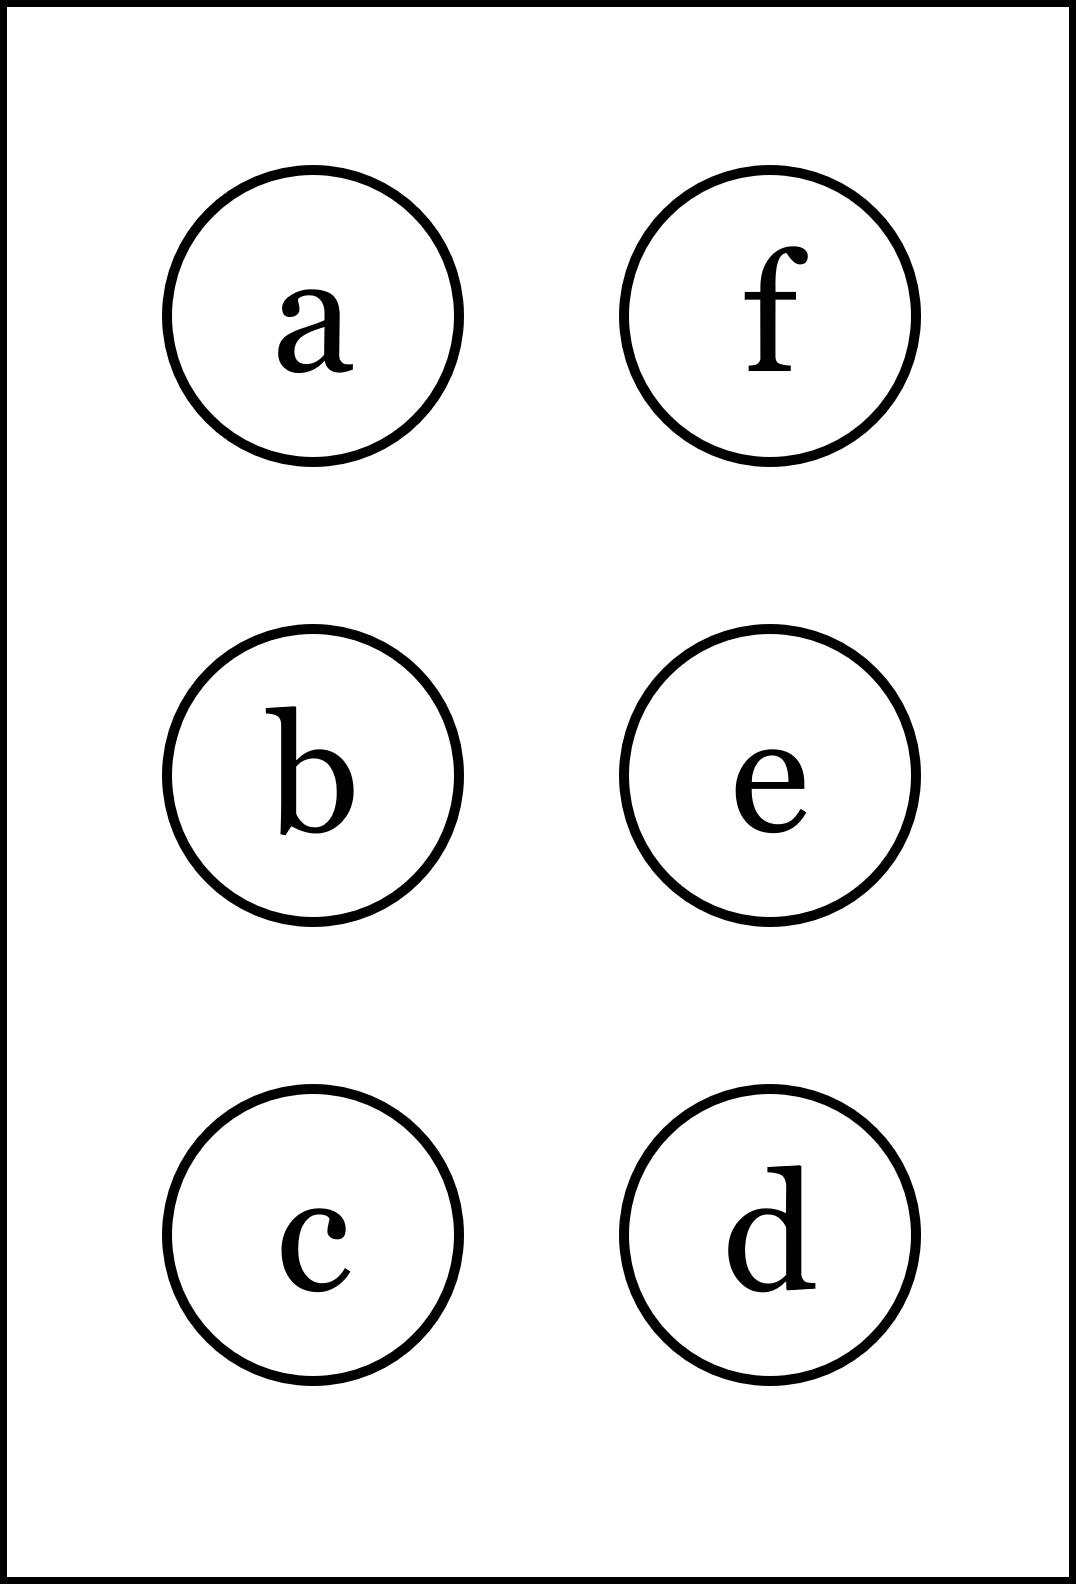
\includegraphics[height=40mm]{../images/braille.png}
{\small Písmeno Braillovej abecedy}
\end{center}
\end{minipage}
\end{center}
\end{minipage}
%
\end{tabular}
\newpage
\thispagestyle{empty}
\begin{tabular}{c:c}
\begin{minipage}[c][104.5mm][t]{0.5\linewidth}
\begin{center}
\vspace{7mm}
{\huge Volné extrémy, skupina \textit{Theta $\theta$} -\romannumeral1}\\[5mm]
\textit{Jméno:}\phantom{xxxxxxxxxxxxxxxxxxxxxxxxxxxxxxxxxxxxxxxxxxxxxxxxxxxxxxxxxxxxxxxxx}\\[5mm]
\begin{minipage}{0.95\linewidth}
\begin{center}
Cílem je najít \textbf{volné extrémy} funkce $f(x,y)$ zadané v \textbf{(a)}.\\Postupuj podle krokú v \textbf{(b)} až \textbf{(f)}. Pokud se medzivýsledky shodujú s těmi za otazníky,\\tak napravo obarvi příslušející kroužek načerno. \textbf{Spolu odevzdejte výsledné slovo}.
\end{center}
\end{minipage}
\\[1mm]
\begin{minipage}{0.79\linewidth}
\begin{center}
\begin{varwidth}{\linewidth}
\begin{enumerate}
\normalsize
\item $f(x,y)=-4x^3-24x^2+60x+4-18y-12y^2-2y^3$\quad \dotfill\; ???\;\dotfill \quad nebarvi
\item Najdi parciální derivaci podle $x$, $\pdv{f}{x}=$\quad \dotfill\; ???\;\dotfill \quad $-12x^2-48x+60$
\item Najdi stacionární body v $x$\quad \dotfill\; ???\;\dotfill \quad $x_1+x_2=-3$
\item Najdi parciální derivaci podle $y$, $\pdv{f}{y}=$\quad \dotfill\; ???\;\dotfill \quad $-6y^2-24y-6$
\item Najdi stacionární body v $y$\quad \dotfill\; ???\;\dotfill \quad $y_1+y_2=-3$
\item Najdi funkční hodnoty vo všech stacionárních bodech \\ \phantom{xxxxxx} a vyber tu najvětší. $f_{\text{max}}(x,y)=$\quad \dotfill\; ???\;\dotfill \quad $44$
\end{enumerate}
\end{varwidth}
\end{center}
\end{minipage}
\begin{minipage}{0.20\linewidth}
\begin{center}
{\Huge\bfseries 1.} \\[2mm]
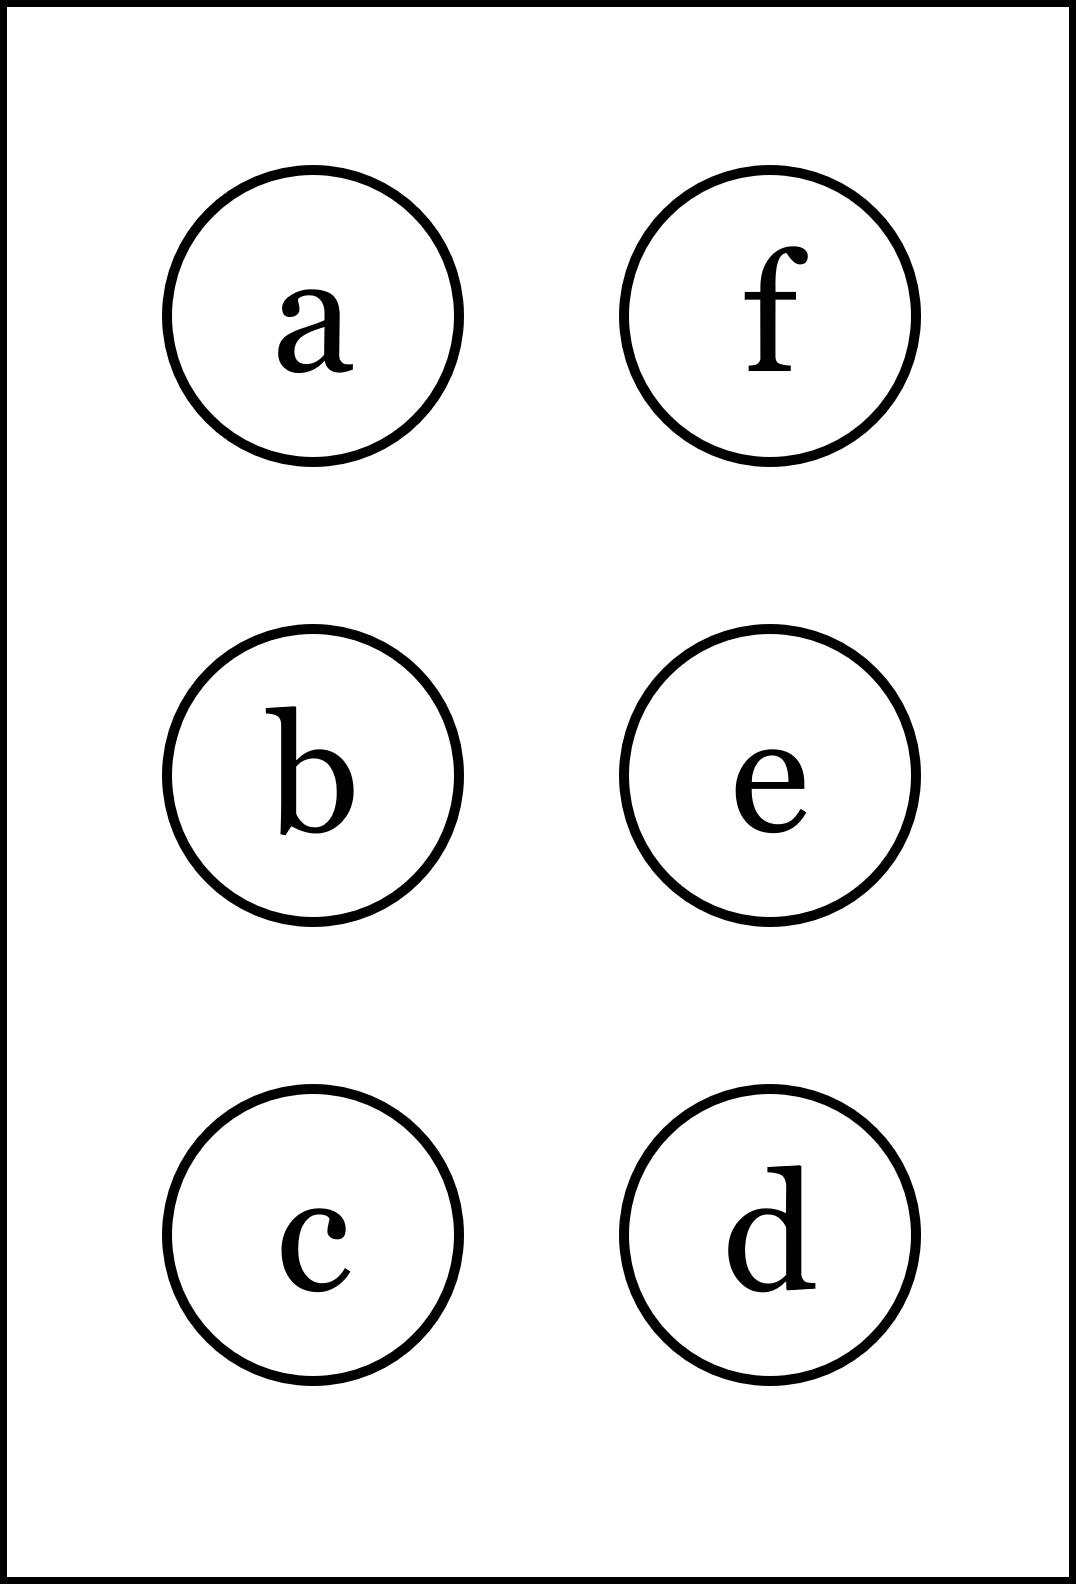
\includegraphics[height=40mm]{../images/braille.png}
{\small Písmeno Braillovej abecedy}
\end{center}
\end{minipage}
\end{center}
\end{minipage}
&
\begin{minipage}[c][104.5mm][t]{0.5\linewidth}
\begin{center}
\vspace{7mm}
{\huge Volné extrémy, skupina \textit{Theta $\theta$} -\romannumeral2}\\[5mm]
\textit{Jméno:}\phantom{xxxxxxxxxxxxxxxxxxxxxxxxxxxxxxxxxxxxxxxxxxxxxxxxxxxxxxxxxxxxxxxxx}\\[5mm]
\begin{minipage}{0.95\linewidth}
\begin{center}
Cílem je najít \textbf{volné extrémy} funkce $f(x,y)$ zadané v \textbf{(a)}.\\Postupuj podle krokú v \textbf{(b)} až \textbf{(f)}. Pokud se medzivýsledky shodujú s těmi za otazníky,\\tak napravo obarvi příslušející kroužek načerno. \textbf{Spolu odevzdejte výsledné slovo}.
\end{center}
\end{minipage}
\\[1mm]
\begin{minipage}{0.79\linewidth}
\begin{center}
\begin{varwidth}{\linewidth}
\begin{enumerate}
\normalsize
\item $f(x,y)=-x^3+9x^2-15x+1+9y+6y^2+y^3$\quad \dotfill\; ???\;\dotfill \quad vybarvi
\item Najdi parciální derivaci podle $x$, $\pdv{f}{x}=$\quad \dotfill\; ???\;\dotfill \quad $-3x^2+18x-15$
\item Najdi stacionární body v $x$\quad \dotfill\; ???\;\dotfill \quad $x_1+x_2=7$
\item Najdi parciální derivaci podle $y$, $\pdv{f}{y}=$\quad \dotfill\; ???\;\dotfill \quad $3y^2+12y+3$
\item Najdi stacionární body v $y$\quad \dotfill\; ???\;\dotfill \quad $y_1+y_2=-4$
\item Najdi funkční hodnoty vo všech stacionárních bodech \\ \phantom{xxxxxx} a vyber tu najvětší. $f_{\text{max}}(x,y)=$\quad \dotfill\; ???\;\dotfill \quad $26$
\end{enumerate}
\end{varwidth}
\end{center}
\end{minipage}
\begin{minipage}{0.20\linewidth}
\begin{center}
{\Huge\bfseries 2.} \\[2mm]
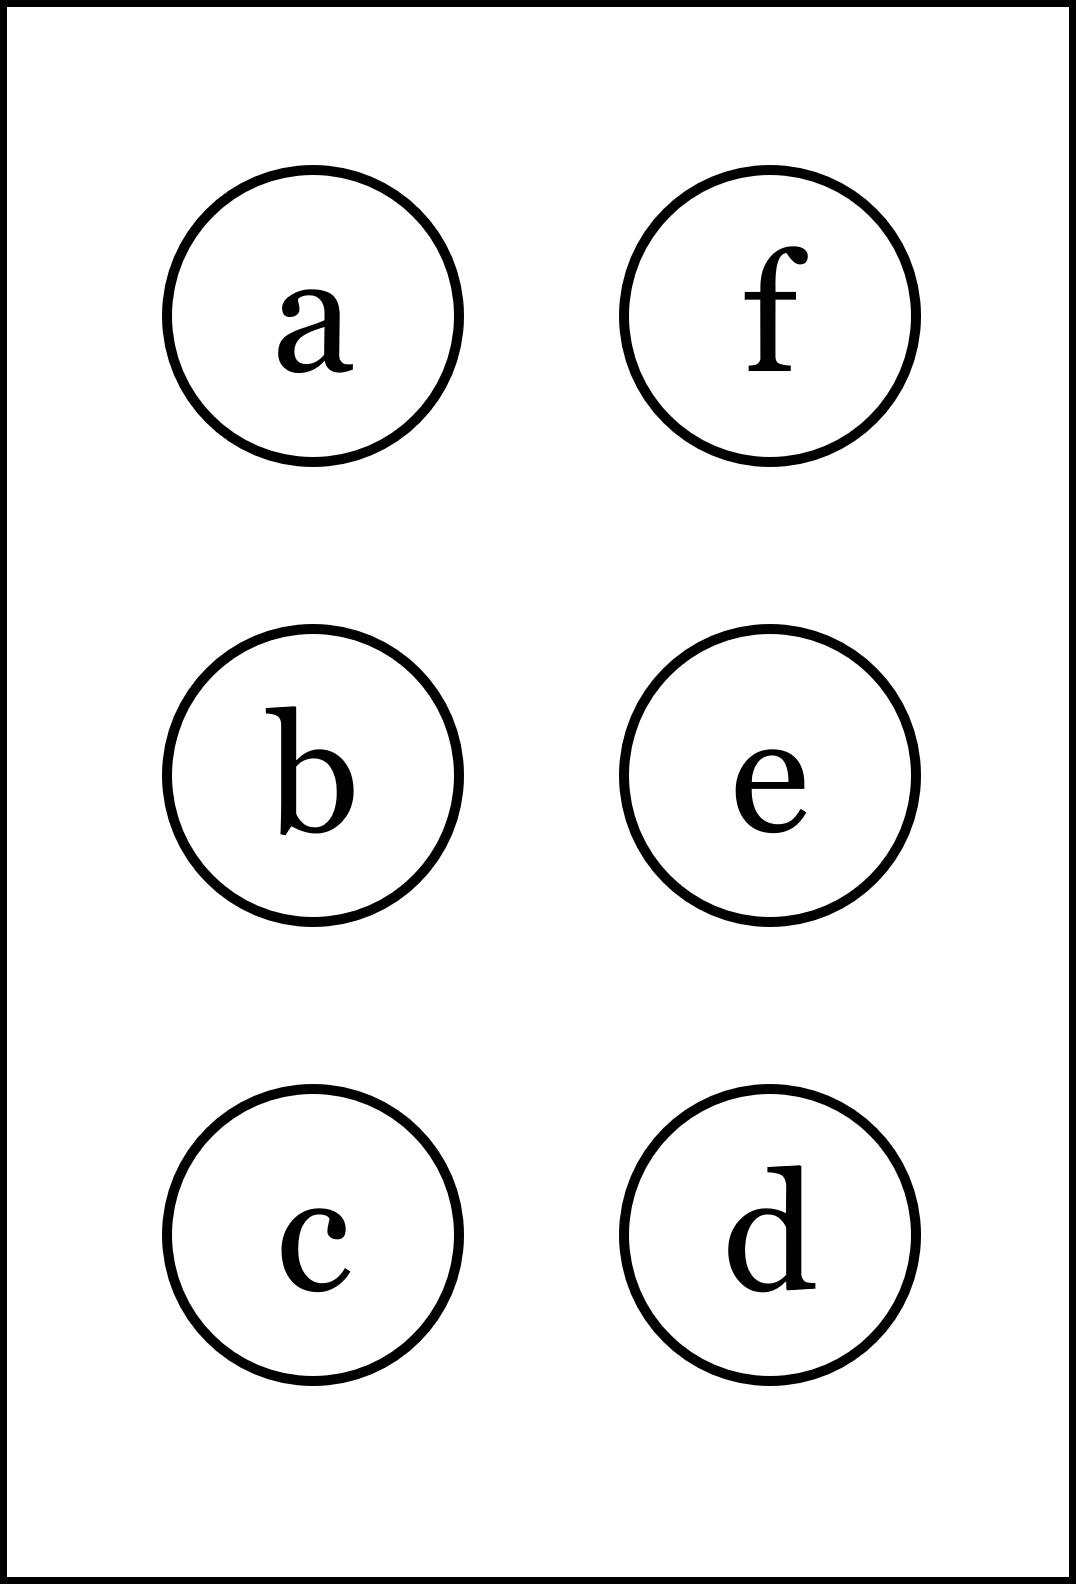
\includegraphics[height=40mm]{../images/braille.png}
{\small Písmeno Braillovej abecedy}
\end{center}
\end{minipage}
\end{center}
\end{minipage}
\\ \hdashline
\begin{minipage}[c][104.5mm][t]{0.5\linewidth}
\begin{center}
\vspace{7mm}
{\huge Volné extrémy, skupina \textit{Theta $\theta$} -\romannumeral3}\\[5mm]
\textit{Jméno:}\phantom{xxxxxxxxxxxxxxxxxxxxxxxxxxxxxxxxxxxxxxxxxxxxxxxxxxxxxxxxxxxxxxxxx}\\[5mm]
\begin{minipage}{0.95\linewidth}
\begin{center}
Cílem je najít \textbf{volné extrémy} funkce $f(x,y)$ zadané v \textbf{(a)}.\\Postupuj podle krokú v \textbf{(b)} až \textbf{(f)}. Pokud se medzivýsledky shodujú s těmi za otazníky,\\tak napravo obarvi příslušející kroužek načerno. \textbf{Spolu odevzdejte výsledné slovo}.
\end{center}
\end{minipage}
\\[1mm]
\begin{minipage}{0.79\linewidth}
\begin{center}
\begin{varwidth}{\linewidth}
\begin{enumerate}
\normalsize
\item $f(x,y)=2x^3-12x^2+18x-7-36y+12y^2+4y^3$\quad \dotfill\; ???\;\dotfill \quad vybarvi
\item Najdi parciální derivaci podle $x$, $\pdv{f}{x}=$\quad \dotfill\; ???\;\dotfill \quad $6x^2-24x+18$
\item Najdi stacionární body v $x$\quad \dotfill\; ???\;\dotfill \quad $x_1+x_2=4$
\item Najdi parciální derivaci podle $y$, $\pdv{f}{y}=$\quad \dotfill\; ???\;\dotfill \quad $12y^2+24y-24$
\item Najdi stacionární body v $y$\quad \dotfill\; ???\;\dotfill \quad $y_1+y_2=-1$
\item Najdi funkční hodnoty vo všech stacionárních bodech \\ \phantom{xxxxxx} a vyber tu najvětší. $f_{\text{max}}(x,y)=$\quad \dotfill\; ???\;\dotfill \quad $-19$
\end{enumerate}
\end{varwidth}
\end{center}
\end{minipage}
\begin{minipage}{0.20\linewidth}
\begin{center}
{\Huge\bfseries 3.} \\[2mm]
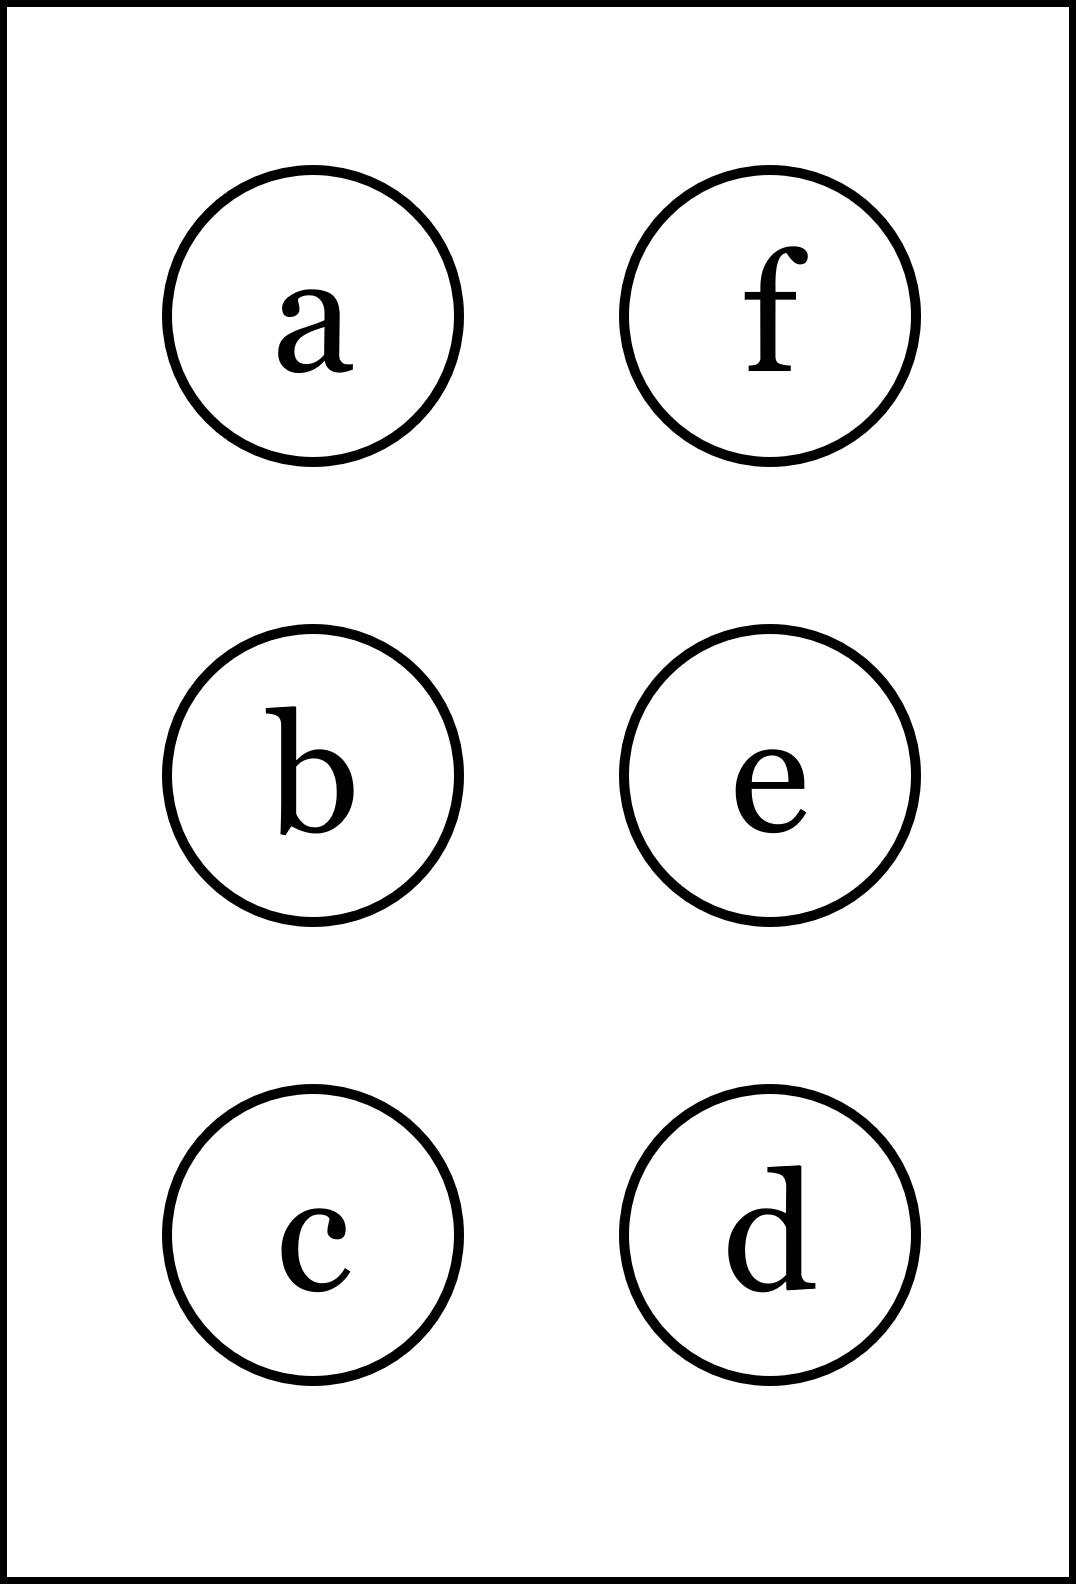
\includegraphics[height=40mm]{../images/braille.png}
{\small Písmeno Braillovej abecedy}
\end{center}
\end{minipage}
\end{center}
\end{minipage}
&
\begin{minipage}[c][104.5mm][t]{0.5\linewidth}
\begin{center}
\vspace{7mm}
{\huge Volné extrémy, skupina \textit{Theta $\theta$} -\romannumeral4}\\[5mm]
\textit{Jméno:}\phantom{xxxxxxxxxxxxxxxxxxxxxxxxxxxxxxxxxxxxxxxxxxxxxxxxxxxxxxxxxxxxxxxxx}\\[5mm]
\begin{minipage}{0.95\linewidth}
\begin{center}
Cílem je najít \textbf{volné extrémy} funkce $f(x,y)$ zadané v \textbf{(a)}.\\Postupuj podle krokú v \textbf{(b)} až \textbf{(f)}. Pokud se medzivýsledky shodujú s těmi za otazníky,\\tak napravo obarvi příslušející kroužek načerno. \textbf{Spolu odevzdejte výsledné slovo}.
\end{center}
\end{minipage}
\\[1mm]
\begin{minipage}{0.79\linewidth}
\begin{center}
\begin{varwidth}{\linewidth}
\begin{enumerate}
\normalsize
\item $f(x,y)=-5x^3+15x^2+45x+1-72y-9y^2+3y^3$\quad \dotfill\; ???\;\dotfill \quad vybarvi
\item Najdi parciální derivaci podle $x$, $\pdv{f}{x}=$\quad \dotfill\; ???\;\dotfill \quad $-15x^2+15x+45$
\item Najdi stacionární body v $x$\quad \dotfill\; ???\;\dotfill \quad $x_1+x_2=2$
\item Najdi parciální derivaci podle $y$, $\pdv{f}{y}=$\quad \dotfill\; ???\;\dotfill \quad $9y^2-18y-72$
\item Najdi stacionární body v $y$\quad \dotfill\; ???\;\dotfill \quad $y_1+y_2=3$
\item Najdi funkční hodnoty vo všech stacionárních bodech \\ \phantom{xxxxxx} a vyber tu najvětší. $f_{\text{max}}(x,y)=$\quad \dotfill\; ???\;\dotfill \quad $-264$
\end{enumerate}
\end{varwidth}
\end{center}
\end{minipage}
\begin{minipage}{0.20\linewidth}
\begin{center}
{\Huge\bfseries 4.} \\[2mm]
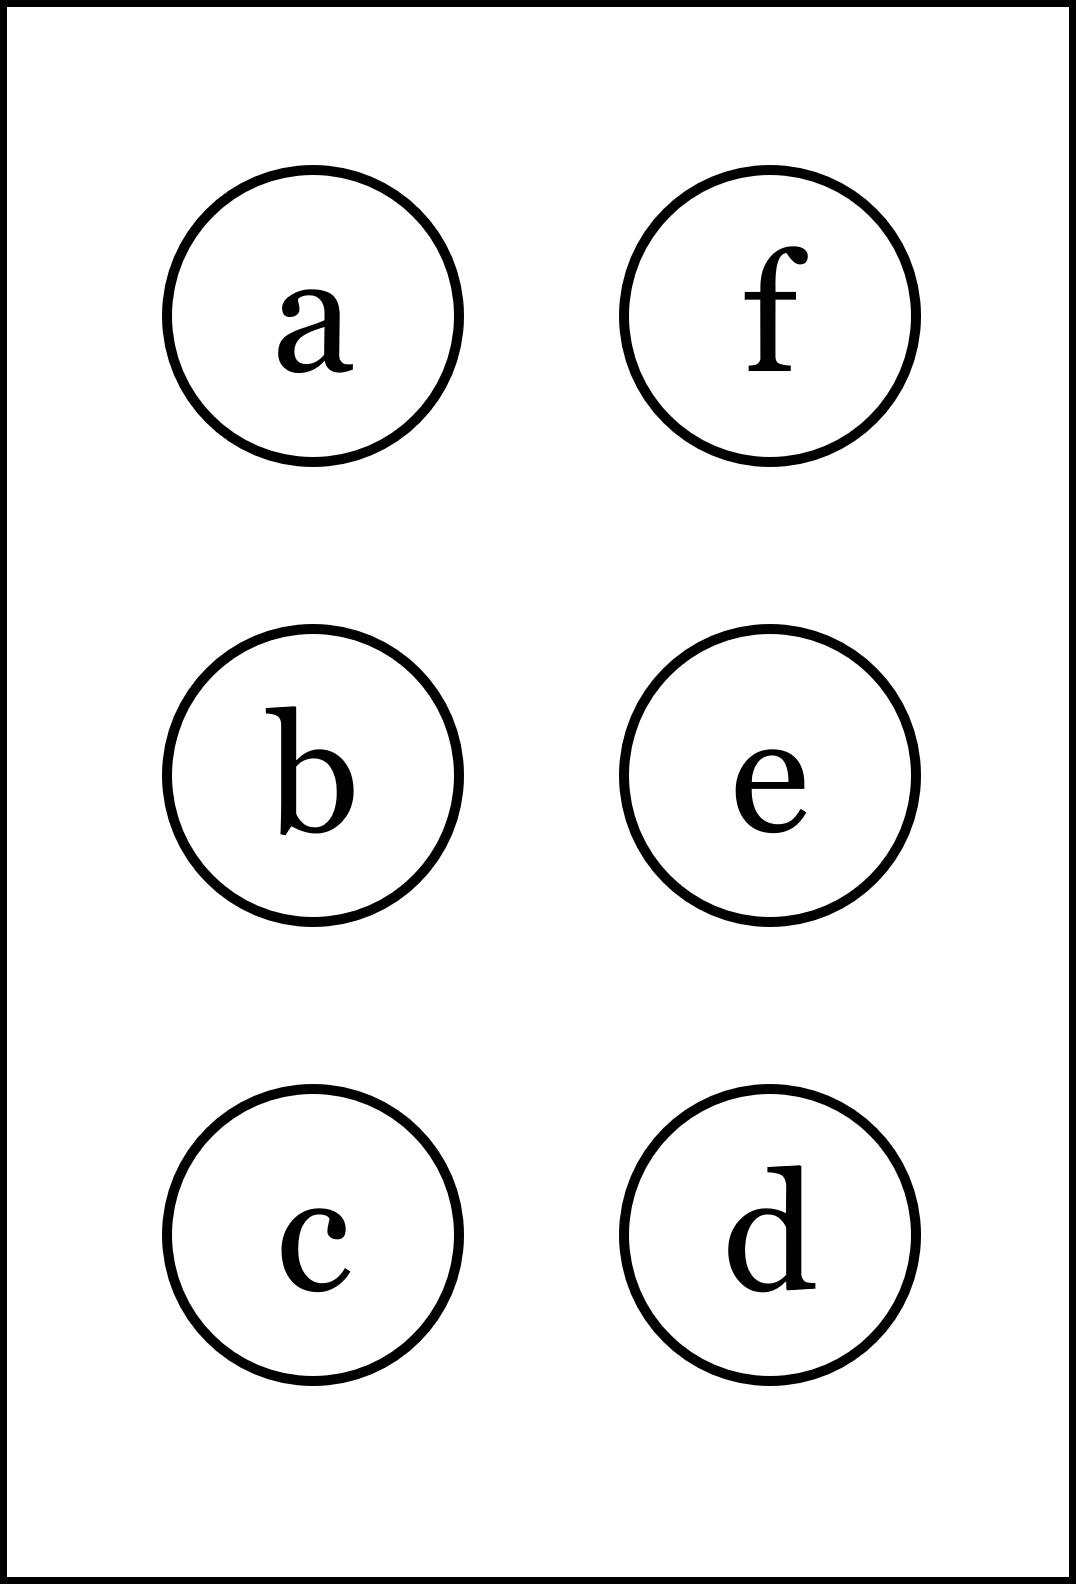
\includegraphics[height=40mm]{../images/braille.png}
{\small Písmeno Braillovej abecedy}
\end{center}
\end{minipage}
\end{center}
\end{minipage}
%
\end{tabular}
\newpage
\thispagestyle{empty}
\begin{tabular}{c:c}
\begin{minipage}[c][104.5mm][t]{0.5\linewidth}
\begin{center}
\vspace{7mm}
{\huge Volné extrémy, skupina \textit{Iota $\iota$} -\romannumeral1}\\[5mm]
\textit{Jméno:}\phantom{xxxxxxxxxxxxxxxxxxxxxxxxxxxxxxxxxxxxxxxxxxxxxxxxxxxxxxxxxxxxxxxxx}\\[5mm]
\begin{minipage}{0.95\linewidth}
\begin{center}
Cílem je najít \textbf{volné extrémy} funkce $f(x,y)$ zadané v \textbf{(a)}.\\Postupuj podle krokú v \textbf{(b)} až \textbf{(f)}. Pokud se medzivýsledky shodujú s těmi za otazníky,\\tak napravo obarvi příslušející kroužek načerno. \textbf{Spolu odevzdejte výsledné slovo}.
\end{center}
\end{minipage}
\\[1mm]
\begin{minipage}{0.79\linewidth}
\begin{center}
\begin{varwidth}{\linewidth}
\begin{enumerate}
\normalsize
\item $f(x,y)=-x^3-3x^2+9x+6-9y+3y^2+y^3$\quad \dotfill\; ???\;\dotfill \quad nebarvi
\item Najdi parciální derivaci podle $x$, $\pdv{f}{x}=$\quad \dotfill\; ???\;\dotfill \quad $-3x^2-3x+9$
\item Najdi stacionární body v $x$\quad \dotfill\; ???\;\dotfill \quad $x_1+x_2=-2$
\item Najdi parciální derivaci podle $y$, $\pdv{f}{y}=$\quad \dotfill\; ???\;\dotfill \quad $3y^2+6y-9$
\item Najdi stacionární body v $y$\quad \dotfill\; ???\;\dotfill \quad $y_1+y_2=-1$
\item Najdi funkční hodnoty vo všech stacionárních bodech \\ \phantom{xxxxxx} a vyber tu najvětší. $f_{\text{max}}(x,y)=$\quad \dotfill\; ???\;\dotfill \quad $38$
\end{enumerate}
\end{varwidth}
\end{center}
\end{minipage}
\begin{minipage}{0.20\linewidth}
\begin{center}
{\Huge\bfseries 1.} \\[2mm]
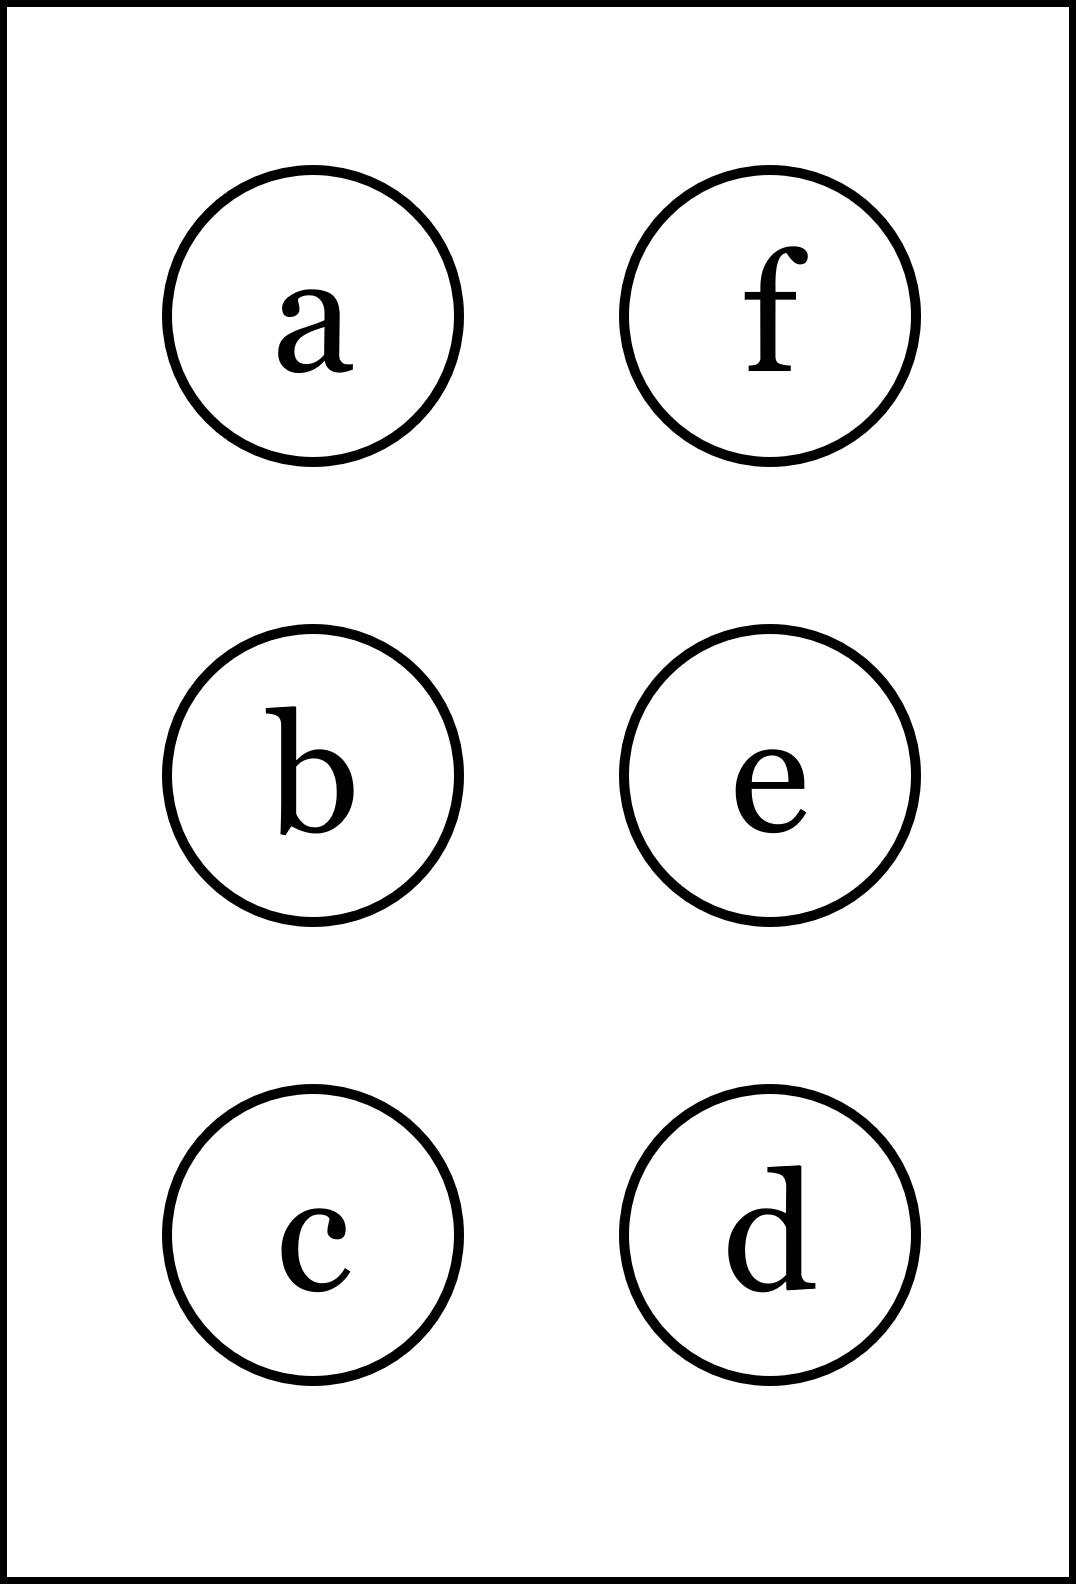
\includegraphics[height=40mm]{../images/braille.png}
{\small Písmeno Braillovej abecedy}
\end{center}
\end{minipage}
\end{center}
\end{minipage}
&
\begin{minipage}[c][104.5mm][t]{0.5\linewidth}
\begin{center}
\vspace{7mm}
{\huge Volné extrémy, skupina \textit{Iota $\iota$} -\romannumeral2}\\[5mm]
\textit{Jméno:}\phantom{xxxxxxxxxxxxxxxxxxxxxxxxxxxxxxxxxxxxxxxxxxxxxxxxxxxxxxxxxxxxxxxxx}\\[5mm]
\begin{minipage}{0.95\linewidth}
\begin{center}
Cílem je najít \textbf{volné extrémy} funkce $f(x,y)$ zadané v \textbf{(a)}.\\Postupuj podle krokú v \textbf{(b)} až \textbf{(f)}. Pokud se medzivýsledky shodujú s těmi za otazníky,\\tak napravo obarvi příslušející kroužek načerno. \textbf{Spolu odevzdejte výsledné slovo}.
\end{center}
\end{minipage}
\\[1mm]
\begin{minipage}{0.79\linewidth}
\begin{center}
\begin{varwidth}{\linewidth}
\begin{enumerate}
\normalsize
\item $f(x,y)=-x^3-6x^2+15x+4+15y-6y^2-y^3$\quad \dotfill\; ???\;\dotfill \quad nebarvi
\item Najdi parciální derivaci podle $x$, $\pdv{f}{x}=$\quad \dotfill\; ???\;\dotfill \quad $-3x^2-12x+15$
\item Najdi stacionární body v $x$\quad \dotfill\; ???\;\dotfill \quad $x_1+x_2=-4$
\item Najdi parciální derivaci podle $y$, $\pdv{f}{y}=$\quad \dotfill\; ???\;\dotfill \quad $-3y^2-12y+9$
\item Najdi stacionární body v $y$\quad \dotfill\; ???\;\dotfill \quad $y_1+y_2=-3$
\item Najdi funkční hodnoty vo všech stacionárních bodech \\ \phantom{xxxxxx} a vyber tu najvětší. $f_{\text{max}}(x,y)=$\quad \dotfill\; ???\;\dotfill \quad $20$
\end{enumerate}
\end{varwidth}
\end{center}
\end{minipage}
\begin{minipage}{0.20\linewidth}
\begin{center}
{\Huge\bfseries 2.} \\[2mm]
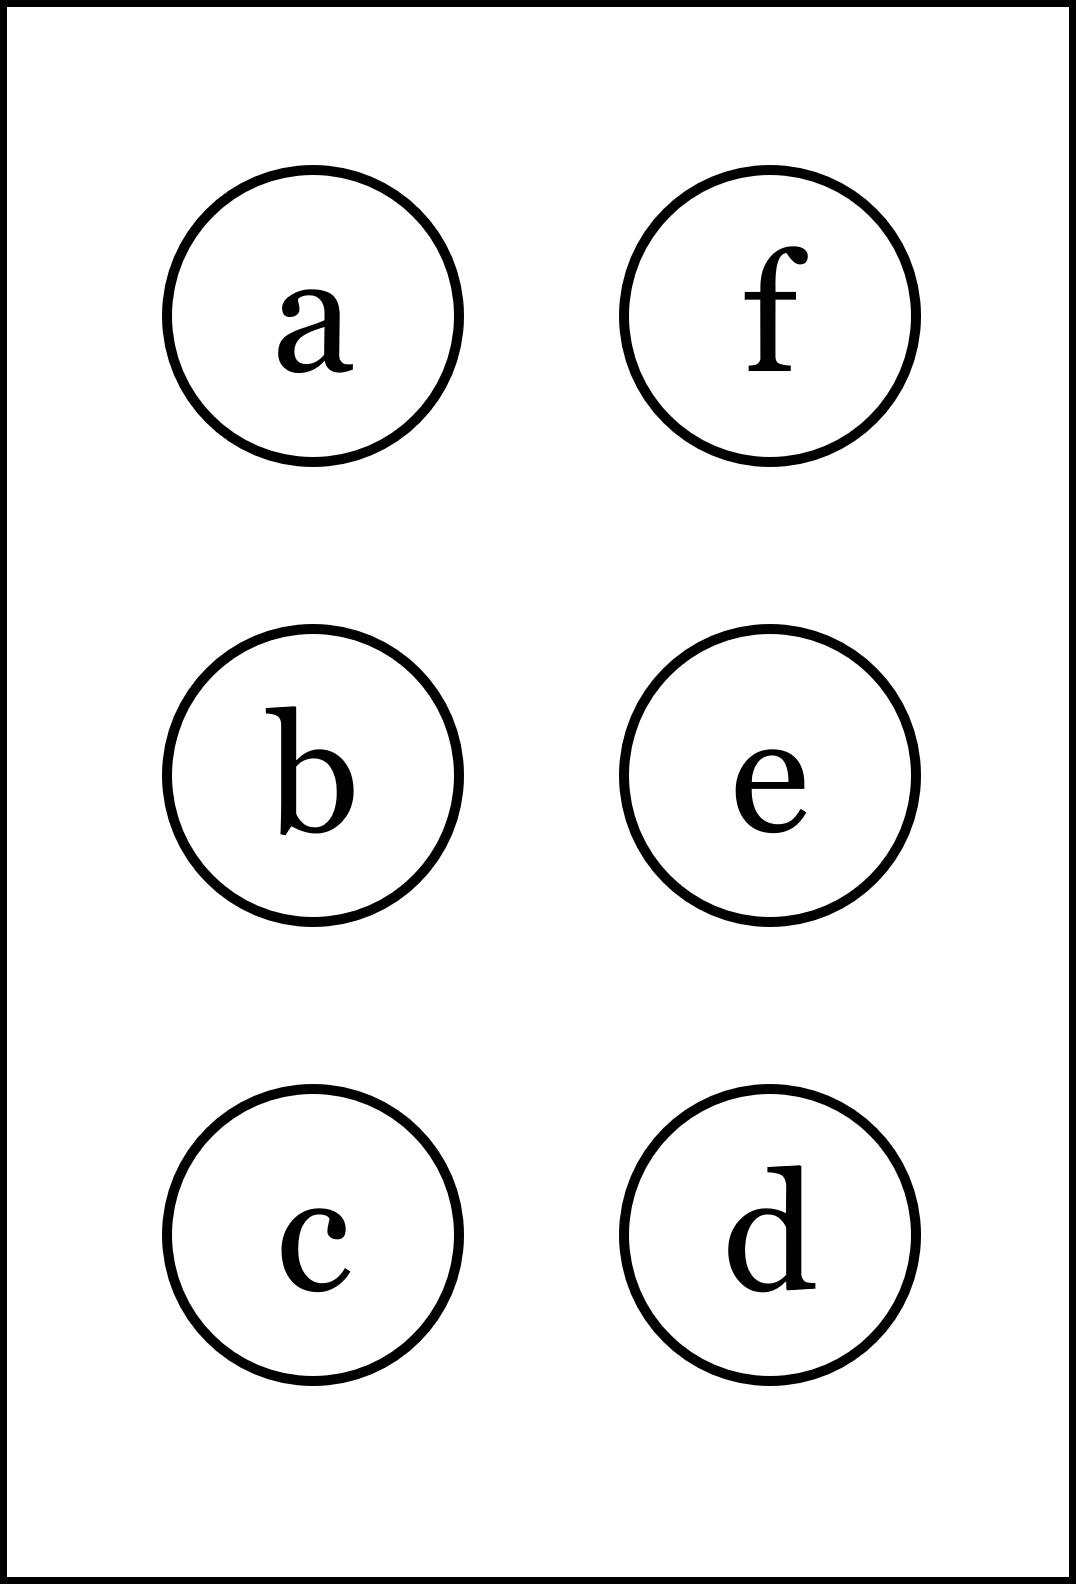
\includegraphics[height=40mm]{../images/braille.png}
{\small Písmeno Braillovej abecedy}
\end{center}
\end{minipage}
\end{center}
\end{minipage}
\\ \hdashline
\begin{minipage}[c][104.5mm][t]{0.5\linewidth}
\begin{center}
\vspace{7mm}
{\huge Volné extrémy, skupina \textit{Iota $\iota$} -\romannumeral3}\\[5mm]
\textit{Jméno:}\phantom{xxxxxxxxxxxxxxxxxxxxxxxxxxxxxxxxxxxxxxxxxxxxxxxxxxxxxxxxxxxxxxxxx}\\[5mm]
\begin{minipage}{0.95\linewidth}
\begin{center}
Cílem je najít \textbf{volné extrémy} funkce $f(x,y)$ zadané v \textbf{(a)}.\\Postupuj podle krokú v \textbf{(b)} až \textbf{(f)}. Pokud se medzivýsledky shodujú s těmi za otazníky,\\tak napravo obarvi příslušející kroužek načerno. \textbf{Spolu odevzdejte výsledné slovo}.
\end{center}
\end{minipage}
\\[1mm]
\begin{minipage}{0.79\linewidth}
\begin{center}
\begin{varwidth}{\linewidth}
\begin{enumerate}
\normalsize
\item $f(x,y)=-4x^3-12x^2+36x+5+45y-3y^2-y^3$\quad \dotfill\; ???\;\dotfill \quad nebarvi
\item Najdi parciální derivaci podle $x$, $\pdv{f}{x}=$\quad \dotfill\; ???\;\dotfill \quad $-12x^2-24x+36$
\item Najdi stacionární body v $x$\quad \dotfill\; ???\;\dotfill \quad $x_1+x_2=-2$
\item Najdi parciální derivaci podle $y$, $\pdv{f}{y}=$\quad \dotfill\; ???\;\dotfill \quad $-3y^2-6y+36$
\item Najdi stacionární body v $y$\quad \dotfill\; ???\;\dotfill \quad $y_1+y_2=-2$
\item Najdi funkční hodnoty vo všech stacionárních bodech \\ \phantom{xxxxxx} a vyber tu najvětší. $f_{\text{max}}(x,y)=$\quad \dotfill\; ???\;\dotfill \quad $106$
\end{enumerate}
\end{varwidth}
\end{center}
\end{minipage}
\begin{minipage}{0.20\linewidth}
\begin{center}
{\Huge\bfseries 3.} \\[2mm]
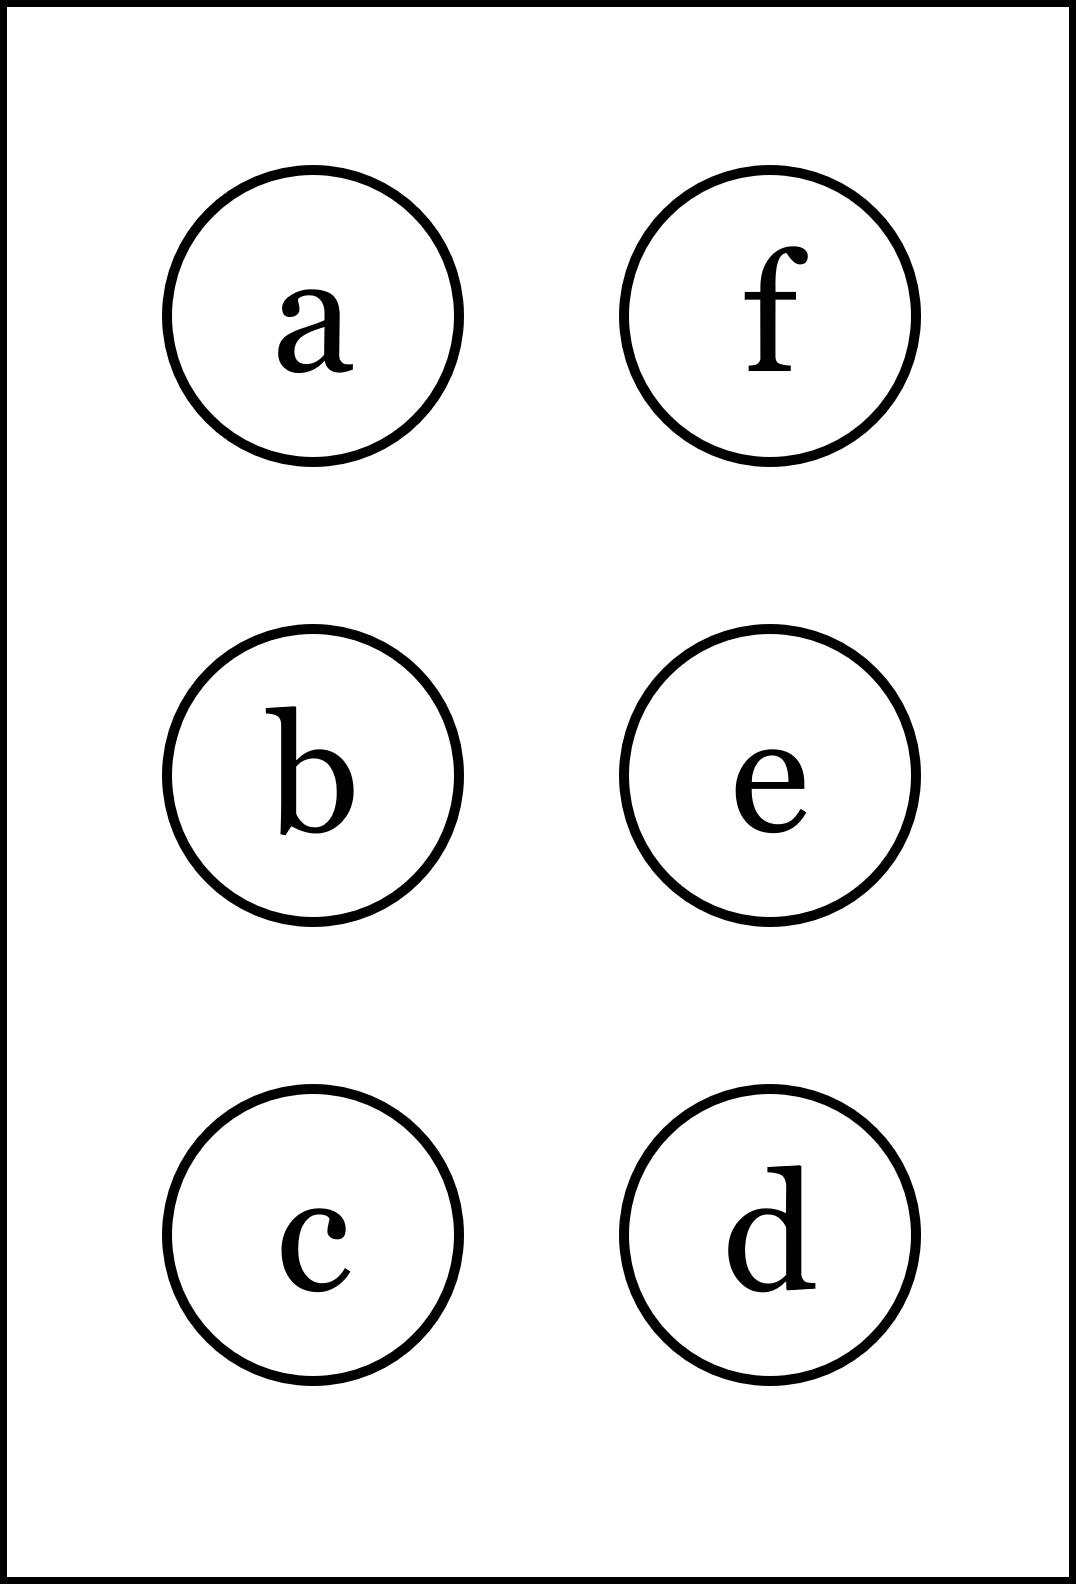
\includegraphics[height=40mm]{../images/braille.png}
{\small Písmeno Braillovej abecedy}
\end{center}
\end{minipage}
\end{center}
\end{minipage}
&
\begin{minipage}[c][104.5mm][t]{0.5\linewidth}
\begin{center}
\vspace{7mm}
{\huge Volné extrémy, skupina \textit{Iota $\iota$} -\romannumeral4}\\[5mm]
\textit{Jméno:}\phantom{xxxxxxxxxxxxxxxxxxxxxxxxxxxxxxxxxxxxxxxxxxxxxxxxxxxxxxxxxxxxxxxxx}\\[5mm]
\begin{minipage}{0.95\linewidth}
\begin{center}
Cílem je najít \textbf{volné extrémy} funkce $f(x,y)$ zadané v \textbf{(a)}.\\Postupuj podle krokú v \textbf{(b)} až \textbf{(f)}. Pokud se medzivýsledky shodujú s těmi za otazníky,\\tak napravo obarvi příslušející kroužek načerno. \textbf{Spolu odevzdejte výsledné slovo}.
\end{center}
\end{minipage}
\\[1mm]
\begin{minipage}{0.79\linewidth}
\begin{center}
\begin{varwidth}{\linewidth}
\begin{enumerate}
\normalsize
\item $f(x,y)=-5x^3-15x^2+45x-2-45y+3y^2+y^3$\quad \dotfill\; ???\;\dotfill \quad vybarvi
\item Najdi parciální derivaci podle $x$, $\pdv{f}{x}=$\quad \dotfill\; ???\;\dotfill \quad $-15x^2-15x+45$
\item Najdi stacionární body v $x$\quad \dotfill\; ???\;\dotfill \quad $x_1+x_2=-1$
\item Najdi parciální derivaci podle $y$, $\pdv{f}{y}=$\quad \dotfill\; ???\;\dotfill \quad $3y^2+6y-36$
\item Najdi stacionární body v $y$\quad \dotfill\; ???\;\dotfill \quad $y_1+y_2=-1$
\item Najdi funkční hodnoty vo všech stacionárních bodech \\ \phantom{xxxxxx} a vyber tu najvětší. $f_{\text{max}}(x,y)=$\quad \dotfill\; ???\;\dotfill \quad $-58$
\end{enumerate}
\end{varwidth}
\end{center}
\end{minipage}
\begin{minipage}{0.20\linewidth}
\begin{center}
{\Huge\bfseries 4.} \\[2mm]
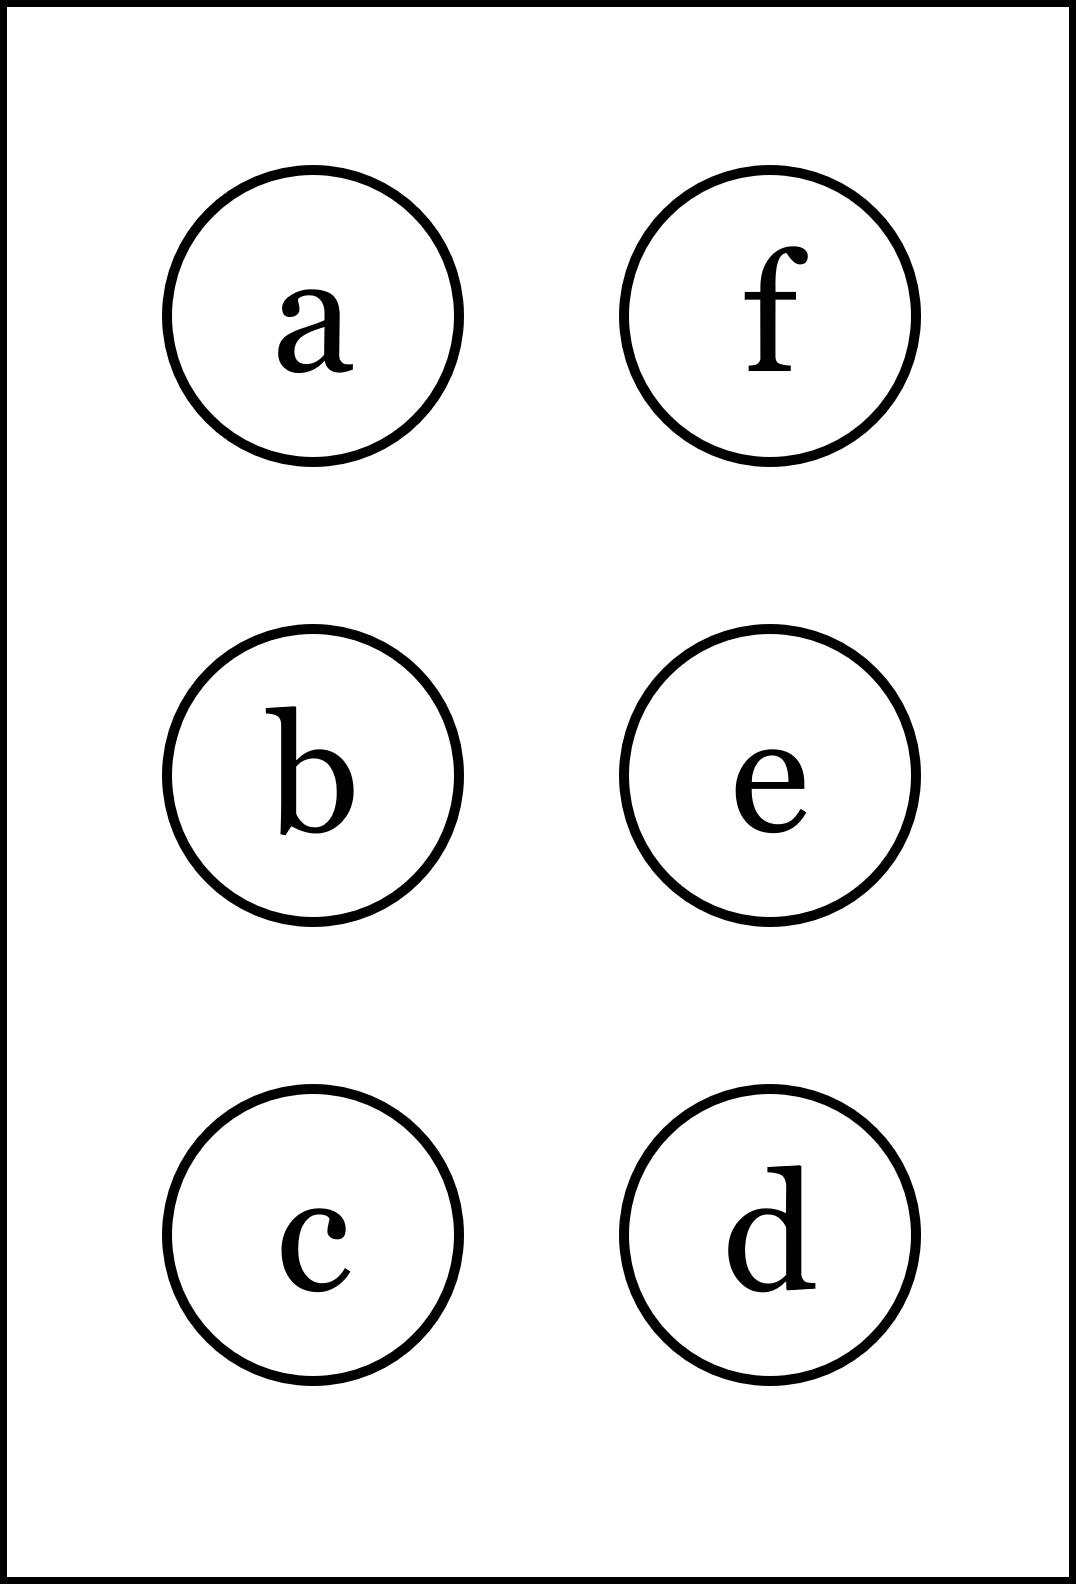
\includegraphics[height=40mm]{../images/braille.png}
{\small Písmeno Braillovej abecedy}
\end{center}
\end{minipage}
\end{center}
\end{minipage}
%
\end{tabular}
\newpage
\thispagestyle{empty}
\begin{tabular}{c:c}
\begin{minipage}[c][104.5mm][t]{0.5\linewidth}
\begin{center}
\vspace{7mm}
{\huge Volné extrémy, skupina \textit{Kappa $\kappa$} -\romannumeral1}\\[5mm]
\textit{Jméno:}\phantom{xxxxxxxxxxxxxxxxxxxxxxxxxxxxxxxxxxxxxxxxxxxxxxxxxxxxxxxxxxxxxxxxx}\\[5mm]
\begin{minipage}{0.95\linewidth}
\begin{center}
Cílem je najít \textbf{volné extrémy} funkce $f(x,y)$ zadané v \textbf{(a)}.\\Postupuj podle krokú v \textbf{(b)} až \textbf{(f)}. Pokud se medzivýsledky shodujú s těmi za otazníky,\\tak napravo obarvi příslušející kroužek načerno. \textbf{Spolu odevzdejte výsledné slovo}.
\end{center}
\end{minipage}
\\[1mm]
\begin{minipage}{0.79\linewidth}
\begin{center}
\begin{varwidth}{\linewidth}
\begin{enumerate}
\normalsize
\item $f(x,y)=-x^3+9x^2+48x+2-48y-9y^2+y^3$\quad \dotfill\; ???\;\dotfill \quad vybarvi
\item Najdi parciální derivaci podle $x$, $\pdv{f}{x}=$\quad \dotfill\; ???\;\dotfill \quad $-3x^2+18x+48$
\item Najdi stacionární body v $x$\quad \dotfill\; ???\;\dotfill \quad $x_1+x_2=6$
\item Najdi parciální derivaci podle $y$, $\pdv{f}{y}=$\quad \dotfill\; ???\;\dotfill \quad $3y^2-18y-30$
\item Najdi stacionární body v $y$\quad \dotfill\; ???\;\dotfill \quad $y_1+y_2=6$
\item Najdi funkční hodnoty vo všech stacionárních bodech \\ \phantom{xxxxxx} a vyber tu najvětší. $f_{\text{max}}(x,y)=$\quad \dotfill\; ???\;\dotfill \quad $-498$
\end{enumerate}
\end{varwidth}
\end{center}
\end{minipage}
\begin{minipage}{0.20\linewidth}
\begin{center}
{\Huge\bfseries 1.} \\[2mm]
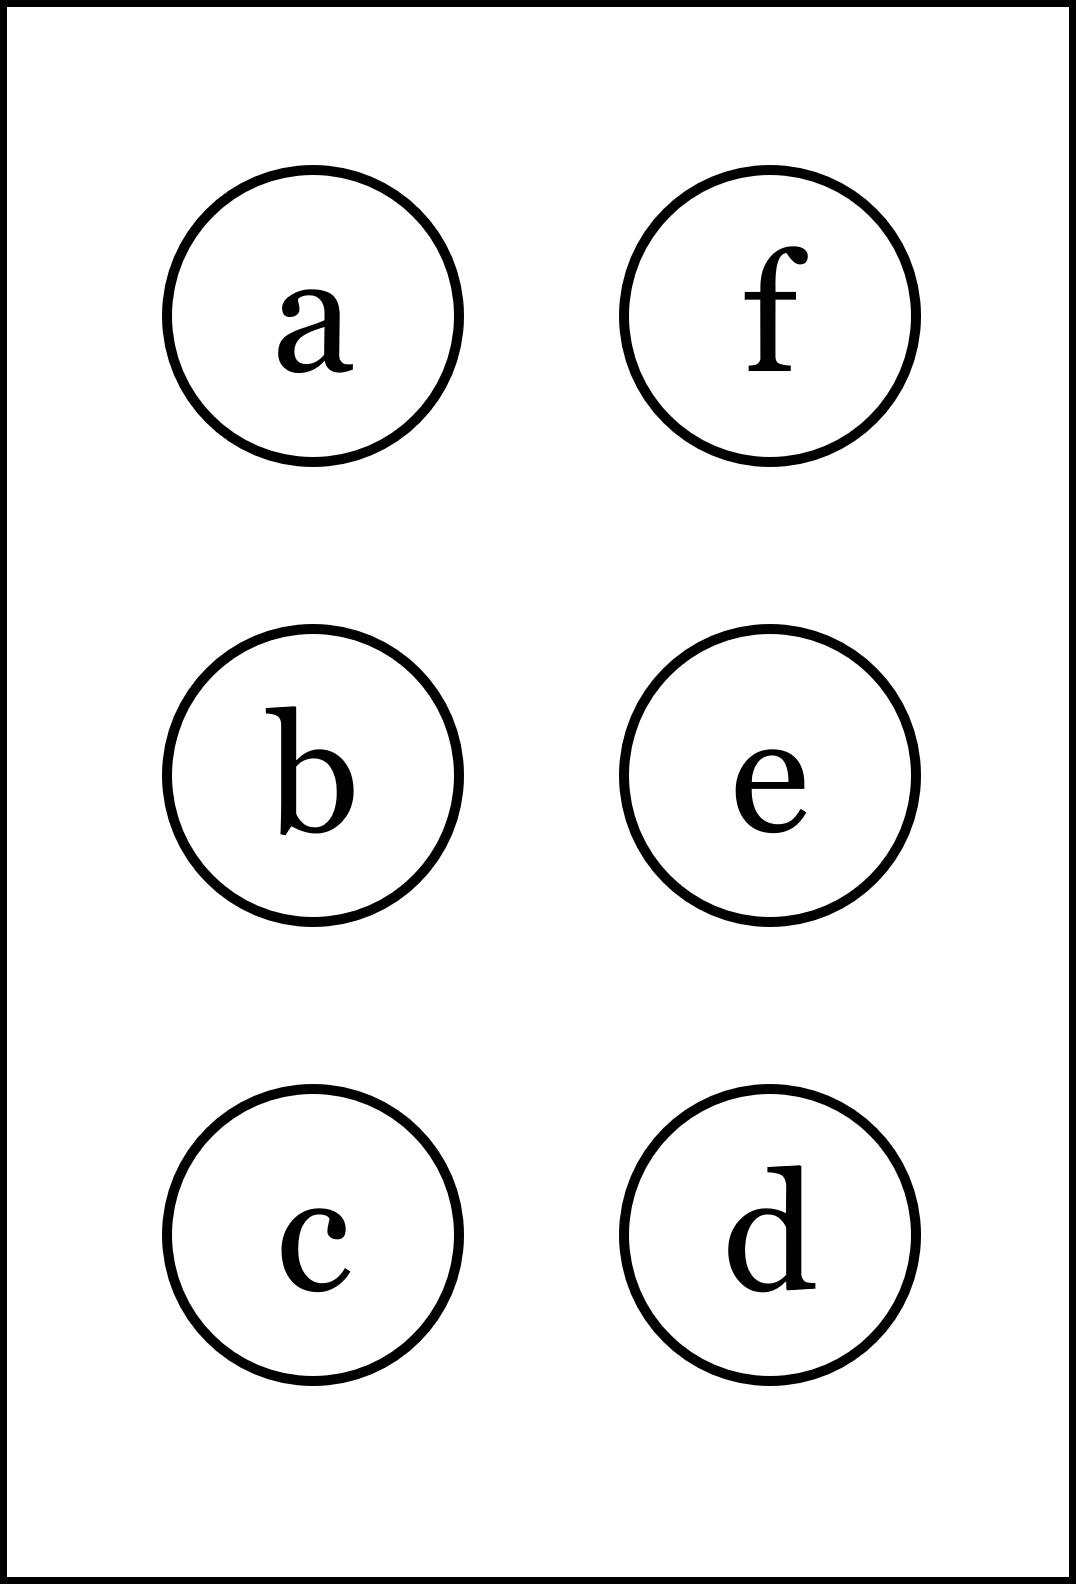
\includegraphics[height=40mm]{../images/braille.png}
{\small Písmeno Braillovej abecedy}
\end{center}
\end{minipage}
\end{center}
\end{minipage}
&
\begin{minipage}[c][104.5mm][t]{0.5\linewidth}
\begin{center}
\vspace{7mm}
{\huge Volné extrémy, skupina \textit{Kappa $\kappa$} -\romannumeral2}\\[5mm]
\textit{Jméno:}\phantom{xxxxxxxxxxxxxxxxxxxxxxxxxxxxxxxxxxxxxxxxxxxxxxxxxxxxxxxxxxxxxxxxx}\\[5mm]
\begin{minipage}{0.95\linewidth}
\begin{center}
Cílem je najít \textbf{volné extrémy} funkce $f(x,y)$ zadané v \textbf{(a)}.\\Postupuj podle krokú v \textbf{(b)} až \textbf{(f)}. Pokud se medzivýsledky shodujú s těmi za otazníky,\\tak napravo obarvi příslušející kroužek načerno. \textbf{Spolu odevzdejte výsledné slovo}.
\end{center}
\end{minipage}
\\[1mm]
\begin{minipage}{0.79\linewidth}
\begin{center}
\begin{varwidth}{\linewidth}
\begin{enumerate}
\normalsize
\item $f(x,y)=2x^3+6x^2-48x+3-15y-6y^2+y^3$\quad \dotfill\; ???\;\dotfill \quad vybarvi
\item Najdi parciální derivaci podle $x$, $\pdv{f}{x}=$\quad \dotfill\; ???\;\dotfill \quad $6x^2+6x-48$
\item Najdi stacionární body v $x$\quad \dotfill\; ???\;\dotfill \quad $x_1+x_2=-2$
\item Najdi parciální derivaci podle $y$, $\pdv{f}{y}=$\quad \dotfill\; ???\;\dotfill \quad $3y^2-12y-15$
\item Najdi stacionární body v $y$\quad \dotfill\; ???\;\dotfill \quad $y_1+y_2=5$
\item Najdi funkční hodnoty vo všech stacionárních bodech \\ \phantom{xxxxxx} a vyber tu najvětší. $f_{\text{max}}(x,y)=$\quad \dotfill\; ???\;\dotfill \quad $-153$
\end{enumerate}
\end{varwidth}
\end{center}
\end{minipage}
\begin{minipage}{0.20\linewidth}
\begin{center}
{\Huge\bfseries 2.} \\[2mm]
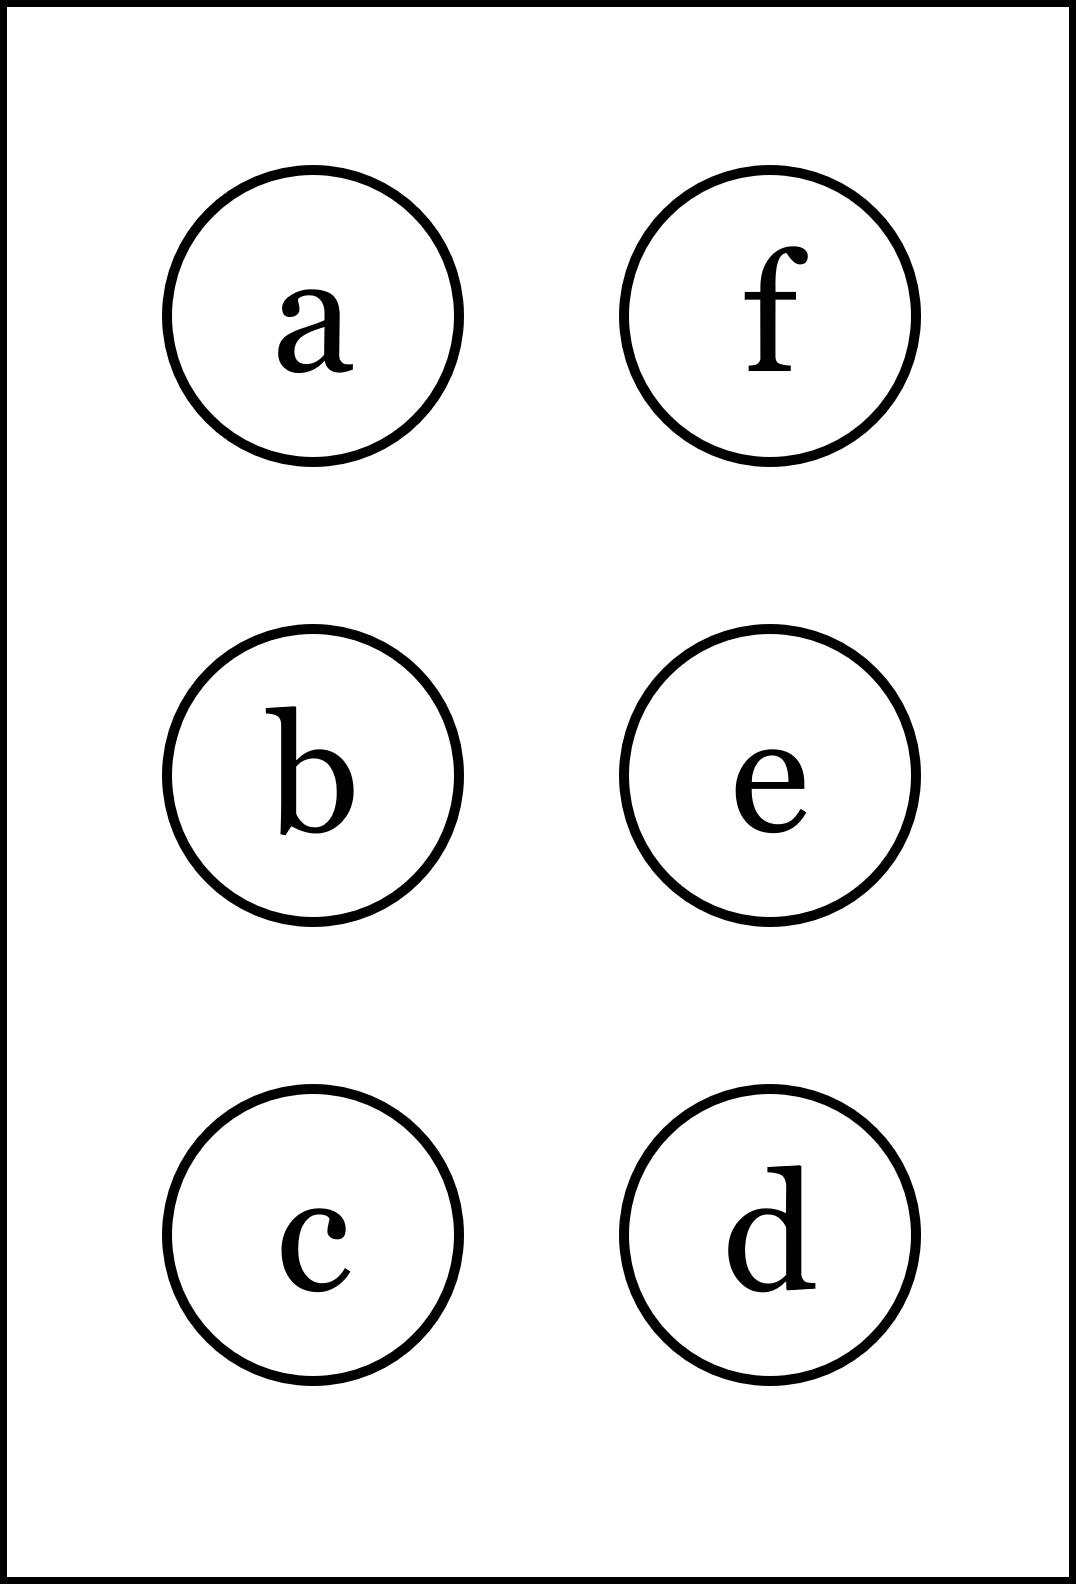
\includegraphics[height=40mm]{../images/braille.png}
{\small Písmeno Braillovej abecedy}
\end{center}
\end{minipage}
\end{center}
\end{minipage}
\\ \hdashline
\begin{minipage}[c][104.5mm][t]{0.5\linewidth}
\begin{center}
\vspace{7mm}
{\huge Volné extrémy, skupina \textit{Kappa $\kappa$} -\romannumeral3}\\[5mm]
\textit{Jméno:}\phantom{xxxxxxxxxxxxxxxxxxxxxxxxxxxxxxxxxxxxxxxxxxxxxxxxxxxxxxxxxxxxxxxxx}\\[5mm]
\begin{minipage}{0.95\linewidth}
\begin{center}
Cílem je najít \textbf{volné extrémy} funkce $f(x,y)$ zadané v \textbf{(a)}.\\Postupuj podle krokú v \textbf{(b)} až \textbf{(f)}. Pokud se medzivýsledky shodujú s těmi za otazníky,\\tak napravo obarvi příslušející kroužek načerno. \textbf{Spolu odevzdejte výsledné slovo}.
\end{center}
\end{minipage}
\\[1mm]
\begin{minipage}{0.79\linewidth}
\begin{center}
\begin{varwidth}{\linewidth}
\begin{enumerate}
\normalsize
\item $f(x,y)=-4x^3-12x^2+36x-6+9y+3y^2-y^3$\quad \dotfill\; ???\;\dotfill \quad vybarvi
\item Najdi parciální derivaci podle $x$, $\pdv{f}{x}=$\quad \dotfill\; ???\;\dotfill \quad $-12x^2-12x+36$
\item Najdi stacionární body v $x$\quad \dotfill\; ???\;\dotfill \quad $x_1+x_2=-2$
\item Najdi parciální derivaci podle $y$, $\pdv{f}{y}=$\quad \dotfill\; ???\;\dotfill \quad $-3y^2+6y+6$
\item Najdi stacionární body v $y$\quad \dotfill\; ???\;\dotfill \quad $y_1+y_2=3$
\item Najdi funkční hodnoty vo všech stacionárních bodech \\ \phantom{xxxxxx} a vyber tu najvětší. $f_{\text{max}}(x,y)=$\quad \dotfill\; ???\;\dotfill \quad $9$
\end{enumerate}
\end{varwidth}
\end{center}
\end{minipage}
\begin{minipage}{0.20\linewidth}
\begin{center}
{\Huge\bfseries 3.} \\[2mm]
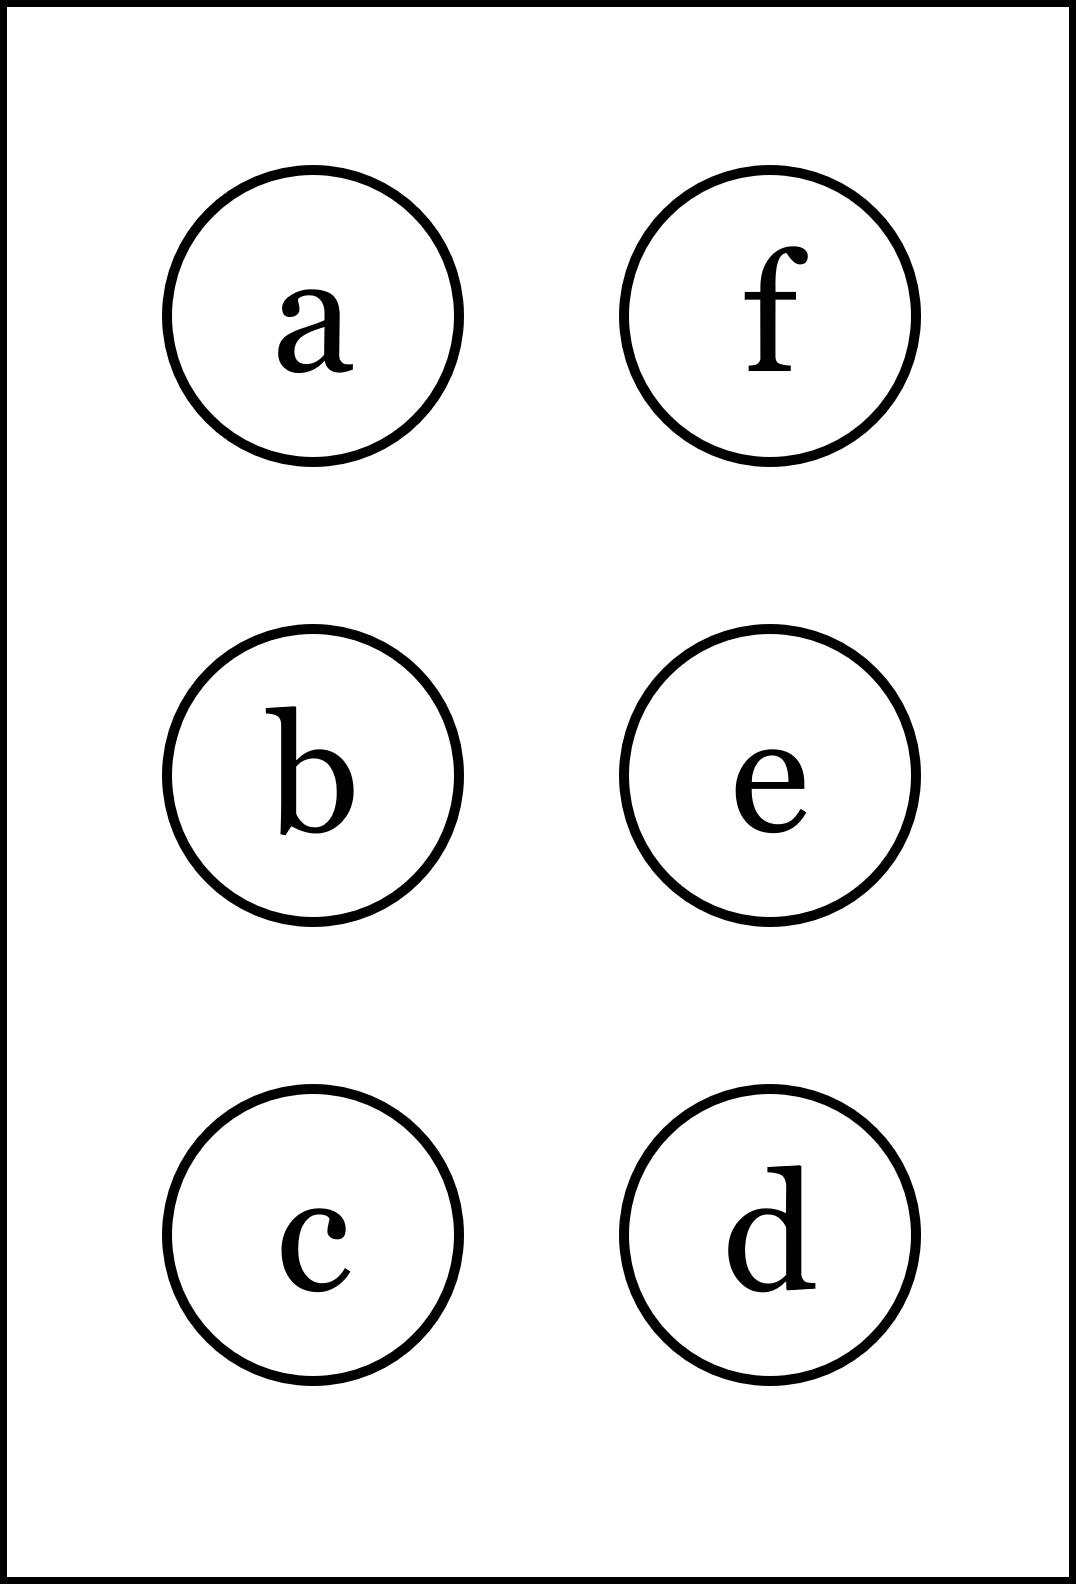
\includegraphics[height=40mm]{../images/braille.png}
{\small Písmeno Braillovej abecedy}
\end{center}
\end{minipage}
\end{center}
\end{minipage}
&
\begin{minipage}[c][104.5mm][t]{0.5\linewidth}
\begin{center}
\vspace{7mm}
{\huge Volné extrémy, skupina \textit{Kappa $\kappa$} -\romannumeral4}\\[5mm]
\textit{Jméno:}\phantom{xxxxxxxxxxxxxxxxxxxxxxxxxxxxxxxxxxxxxxxxxxxxxxxxxxxxxxxxxxxxxxxxx}\\[5mm]
\begin{minipage}{0.95\linewidth}
\begin{center}
Cílem je najít \textbf{volné extrémy} funkce $f(x,y)$ zadané v \textbf{(a)}.\\Postupuj podle krokú v \textbf{(b)} až \textbf{(f)}. Pokud se medzivýsledky shodujú s těmi za otazníky,\\tak napravo obarvi příslušející kroužek načerno. \textbf{Spolu odevzdejte výsledné slovo}.
\end{center}
\end{minipage}
\\[1mm]
\begin{minipage}{0.79\linewidth}
\begin{center}
\begin{varwidth}{\linewidth}
\begin{enumerate}
\normalsize
\item $f(x,y)=-x^3-6x^2-9x+5-18y-6y^2+2y^3$\quad \dotfill\; ???\;\dotfill \quad vybarvi
\item Najdi parciální derivaci podle $x$, $\pdv{f}{x}=$\quad \dotfill\; ???\;\dotfill \quad $-3x^2-6x-9$
\item Najdi stacionární body v $x$\quad \dotfill\; ???\;\dotfill \quad $x_1+x_2=-3$
\item Najdi parciální derivaci podle $y$, $\pdv{f}{y}=$\quad \dotfill\; ???\;\dotfill \quad $6y^2-12y-12$
\item Najdi stacionární body v $y$\quad \dotfill\; ???\;\dotfill \quad $y_1+y_2=3$
\item Najdi funkční hodnoty vo všech stacionárních bodech \\ \phantom{xxxxxx} a vyber tu najvětší. $f_{\text{max}}(x,y)=$\quad \dotfill\; ???\;\dotfill \quad $-49$
\end{enumerate}
\end{varwidth}
\end{center}
\end{minipage}
\begin{minipage}{0.20\linewidth}
\begin{center}
{\Huge\bfseries 4.} \\[2mm]
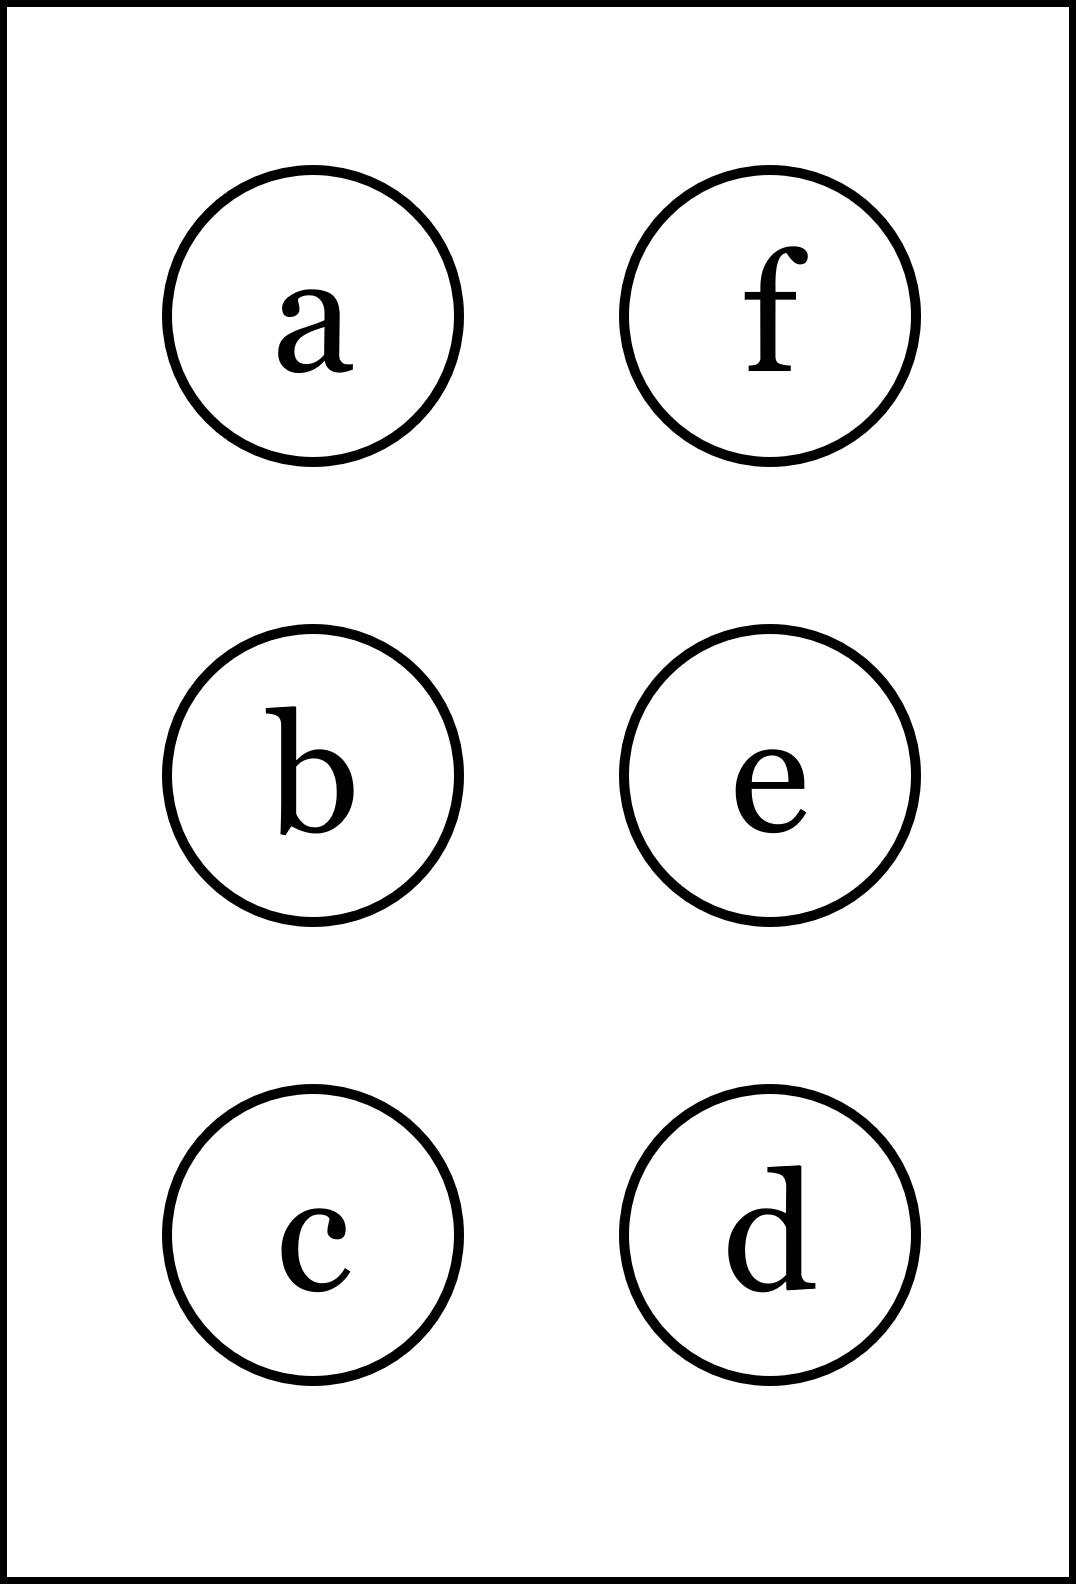
\includegraphics[height=40mm]{../images/braille.png}
{\small Písmeno Braillovej abecedy}
\end{center}
\end{minipage}
\end{center}
\end{minipage}
%
\end{tabular}
\newpage
\thispagestyle{empty}
\begin{tabular}{c:c}
\begin{minipage}[c][104.5mm][t]{0.5\linewidth}
\begin{center}
\vspace{7mm}
{\huge Volné extrémy, skupina \textit{Lambda $\lambda$} -\romannumeral1}\\[5mm]
\textit{Jméno:}\phantom{xxxxxxxxxxxxxxxxxxxxxxxxxxxxxxxxxxxxxxxxxxxxxxxxxxxxxxxxxxxxxxxxx}\\[5mm]
\begin{minipage}{0.95\linewidth}
\begin{center}
Cílem je najít \textbf{volné extrémy} funkce $f(x,y)$ zadané v \textbf{(a)}.\\Postupuj podle krokú v \textbf{(b)} až \textbf{(f)}. Pokud se medzivýsledky shodujú s těmi za otazníky,\\tak napravo obarvi příslušející kroužek načerno. \textbf{Spolu odevzdejte výsledné slovo}.
\end{center}
\end{minipage}
\\[1mm]
\begin{minipage}{0.79\linewidth}
\begin{center}
\begin{varwidth}{\linewidth}
\begin{enumerate}
\normalsize
\item $f(x,y)=x^3+9x^2+15x-1+72y+9y^2-3y^3$\quad \dotfill\; ???\;\dotfill \quad vybarvi
\item Najdi parciální derivaci podle $x$, $\pdv{f}{x}=$\quad \dotfill\; ???\;\dotfill \quad $3x^2+9x+15$
\item Najdi stacionární body v $x$\quad \dotfill\; ???\;\dotfill \quad $x_1+x_2=-6$
\item Najdi parciální derivaci podle $y$, $\pdv{f}{y}=$\quad \dotfill\; ???\;\dotfill \quad $-9y^2+18y+72$
\item Najdi stacionární body v $y$\quad \dotfill\; ???\;\dotfill \quad $y_1+y_2=2$
\item Najdi funkční hodnoty vo všech stacionárních bodech \\ \phantom{xxxxxx} a vyber tu najvětší. $f_{\text{max}}(x,y)=$\quad \dotfill\; ???\;\dotfill \quad $-60$
\end{enumerate}
\end{varwidth}
\end{center}
\end{minipage}
\begin{minipage}{0.20\linewidth}
\begin{center}
{\Huge\bfseries 1.} \\[2mm]
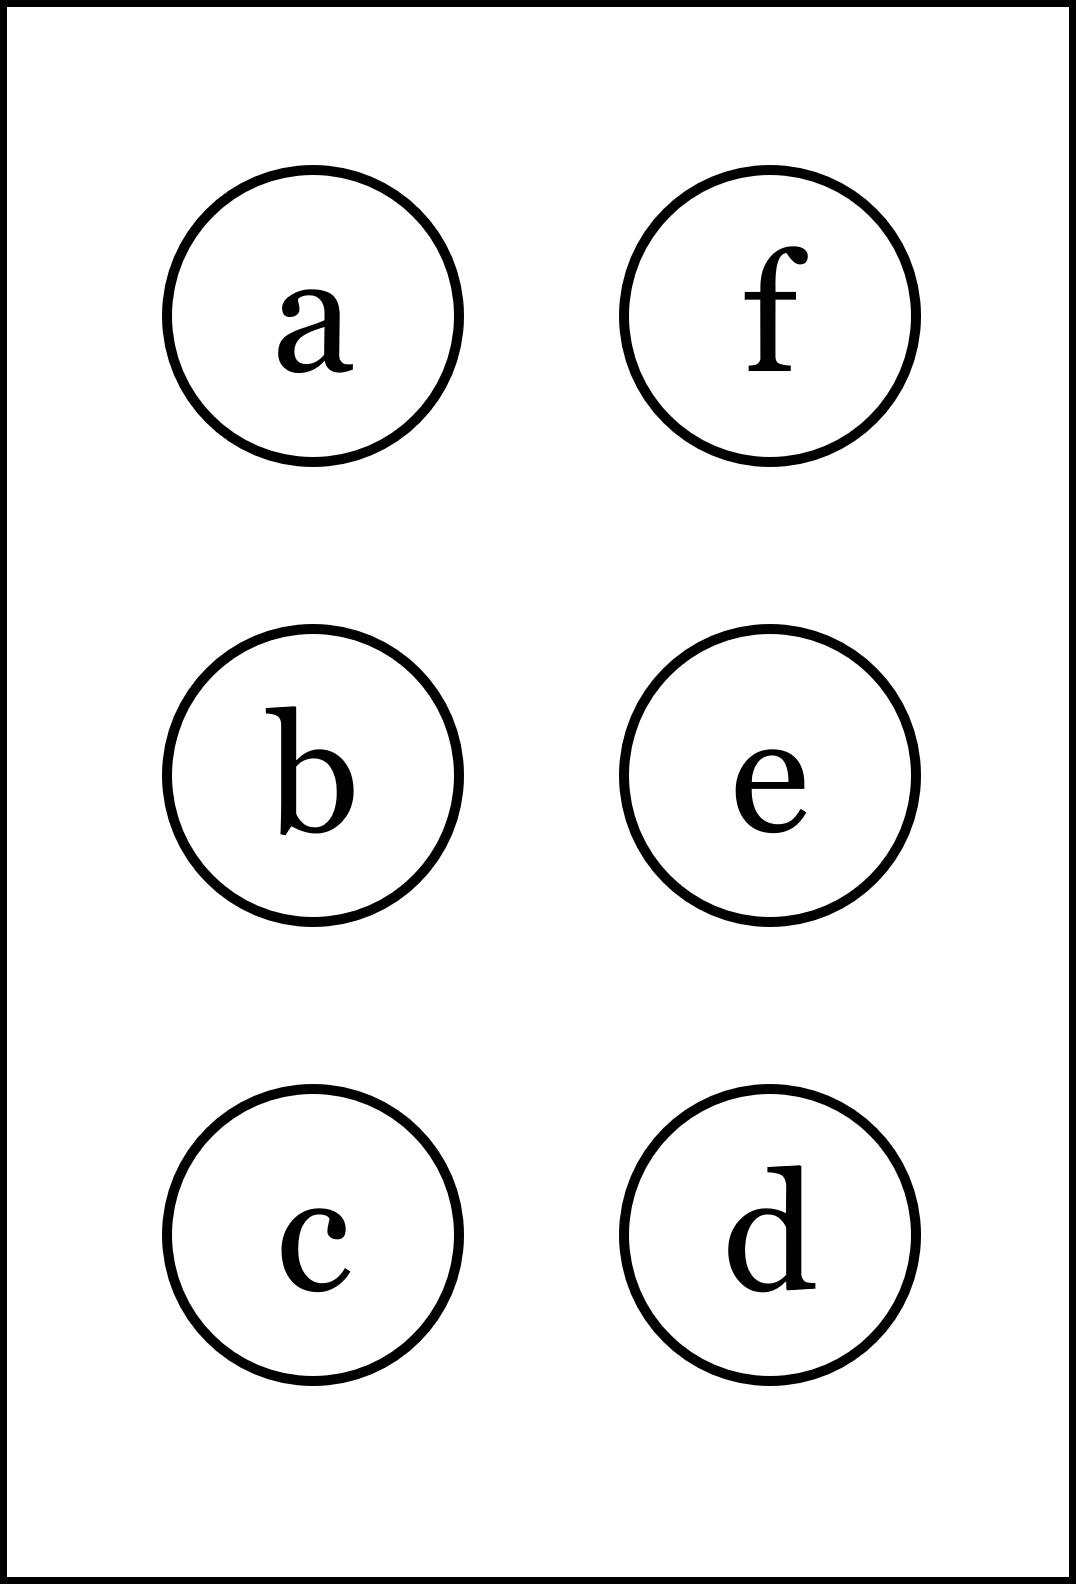
\includegraphics[height=40mm]{../images/braille.png}
{\small Písmeno Braillovej abecedy}
\end{center}
\end{minipage}
\end{center}
\end{minipage}
&
\begin{minipage}[c][104.5mm][t]{0.5\linewidth}
\begin{center}
\vspace{7mm}
{\huge Volné extrémy, skupina \textit{Lambda $\lambda$} -\romannumeral2}\\[5mm]
\textit{Jméno:}\phantom{xxxxxxxxxxxxxxxxxxxxxxxxxxxxxxxxxxxxxxxxxxxxxxxxxxxxxxxxxxxxxxxxx}\\[5mm]
\begin{minipage}{0.95\linewidth}
\begin{center}
Cílem je najít \textbf{volné extrémy} funkce $f(x,y)$ zadané v \textbf{(a)}.\\Postupuj podle krokú v \textbf{(b)} až \textbf{(f)}. Pokud se medzivýsledky shodujú s těmi za otazníky,\\tak napravo obarvi příslušející kroužek načerno. \textbf{Spolu odevzdejte výsledné slovo}.
\end{center}
\end{minipage}
\\[1mm]
\begin{minipage}{0.79\linewidth}
\begin{center}
\begin{varwidth}{\linewidth}
\begin{enumerate}
\normalsize
\item $f(x,y)=3x^3+9x^2-27x-3-18y+6y^2+2y^3$\quad \dotfill\; ???\;\dotfill \quad nebarvi
\item Najdi parciální derivaci podle $x$, $\pdv{f}{x}=$\quad \dotfill\; ???\;\dotfill \quad $9x^2+18x-27$
\item Najdi stacionární body v $x$\quad \dotfill\; ???\;\dotfill \quad $x_1+x_2=-1$
\item Najdi parciální derivaci podle $y$, $\pdv{f}{y}=$\quad \dotfill\; ???\;\dotfill \quad $6y^2+12y-12$
\item Najdi stacionární body v $y$\quad \dotfill\; ???\;\dotfill \quad $y_1+y_2=-1$
\item Najdi funkční hodnoty vo všech stacionárních bodech \\ \phantom{xxxxxx} a vyber tu najvětší. $f_{\text{max}}(x,y)=$\quad \dotfill\; ???\;\dotfill \quad $132$
\end{enumerate}
\end{varwidth}
\end{center}
\end{minipage}
\begin{minipage}{0.20\linewidth}
\begin{center}
{\Huge\bfseries 2.} \\[2mm]
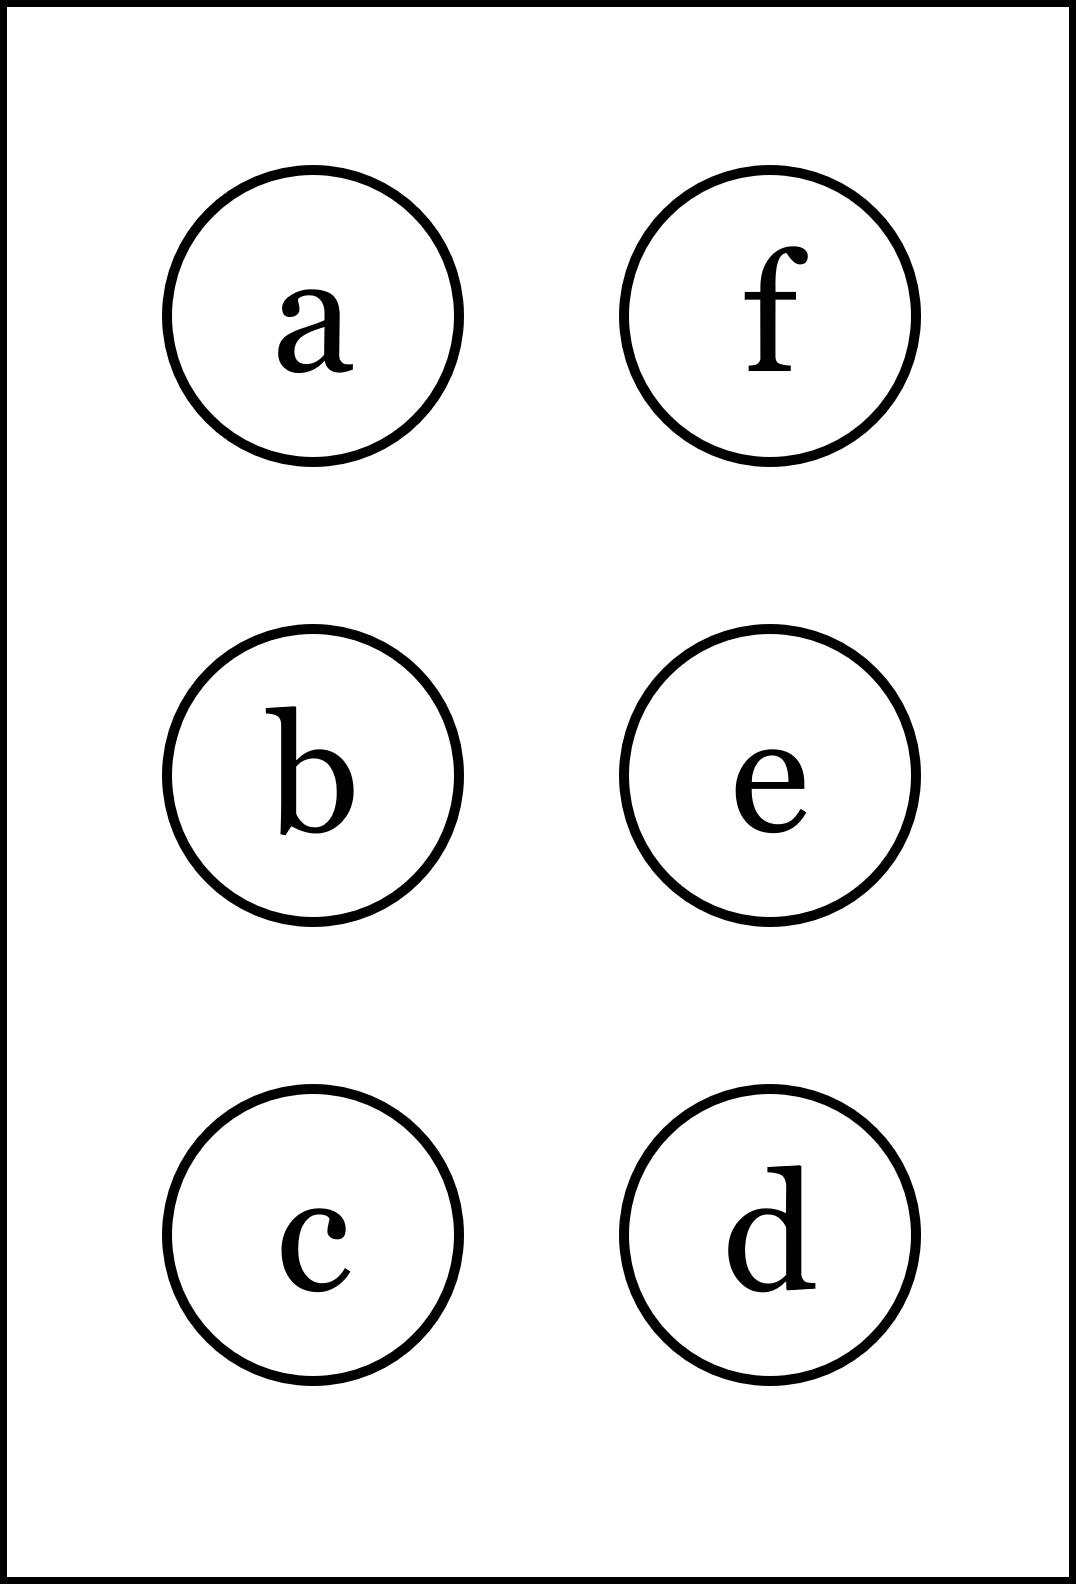
\includegraphics[height=40mm]{../images/braille.png}
{\small Písmeno Braillovej abecedy}
\end{center}
\end{minipage}
\end{center}
\end{minipage}
\\ \hdashline
\begin{minipage}[c][104.5mm][t]{0.5\linewidth}
\begin{center}
\vspace{7mm}
{\huge Volné extrémy, skupina \textit{Lambda $\lambda$} -\romannumeral3}\\[5mm]
\textit{Jméno:}\phantom{xxxxxxxxxxxxxxxxxxxxxxxxxxxxxxxxxxxxxxxxxxxxxxxxxxxxxxxxxxxxxxxxx}\\[5mm]
\begin{minipage}{0.95\linewidth}
\begin{center}
Cílem je najít \textbf{volné extrémy} funkce $f(x,y)$ zadané v \textbf{(a)}.\\Postupuj podle krokú v \textbf{(b)} až \textbf{(f)}. Pokud se medzivýsledky shodujú s těmi za otazníky,\\tak napravo obarvi příslušející kroužek načerno. \textbf{Spolu odevzdejte výsledné slovo}.
\end{center}
\end{minipage}
\\[1mm]
\begin{minipage}{0.79\linewidth}
\begin{center}
\begin{varwidth}{\linewidth}
\begin{enumerate}
\normalsize
\item $f(x,y)=-3x^3+9x^2+27x-5+21y+9y^2-y^3$\quad \dotfill\; ???\;\dotfill \quad vybarvi
\item Najdi parciální derivaci podle $x$, $\pdv{f}{x}=$\quad \dotfill\; ???\;\dotfill \quad $-9x^2+9x+27$
\item Najdi stacionární body v $x$\quad \dotfill\; ???\;\dotfill \quad $x_1+x_2=2$
\item Najdi parciální derivaci podle $y$, $\pdv{f}{y}=$\quad \dotfill\; ???\;\dotfill \quad $-3y^2+18y+12$
\item Najdi stacionární body v $y$\quad \dotfill\; ???\;\dotfill \quad $y_1+y_2=7$
\item Najdi funkční hodnoty vo všech stacionárních bodech \\ \phantom{xxxxxx} a vyber tu najvětší. $f_{\text{max}}(x,y)=$\quad \dotfill\; ???\;\dotfill \quad $321$
\end{enumerate}
\end{varwidth}
\end{center}
\end{minipage}
\begin{minipage}{0.20\linewidth}
\begin{center}
{\Huge\bfseries 3.} \\[2mm]
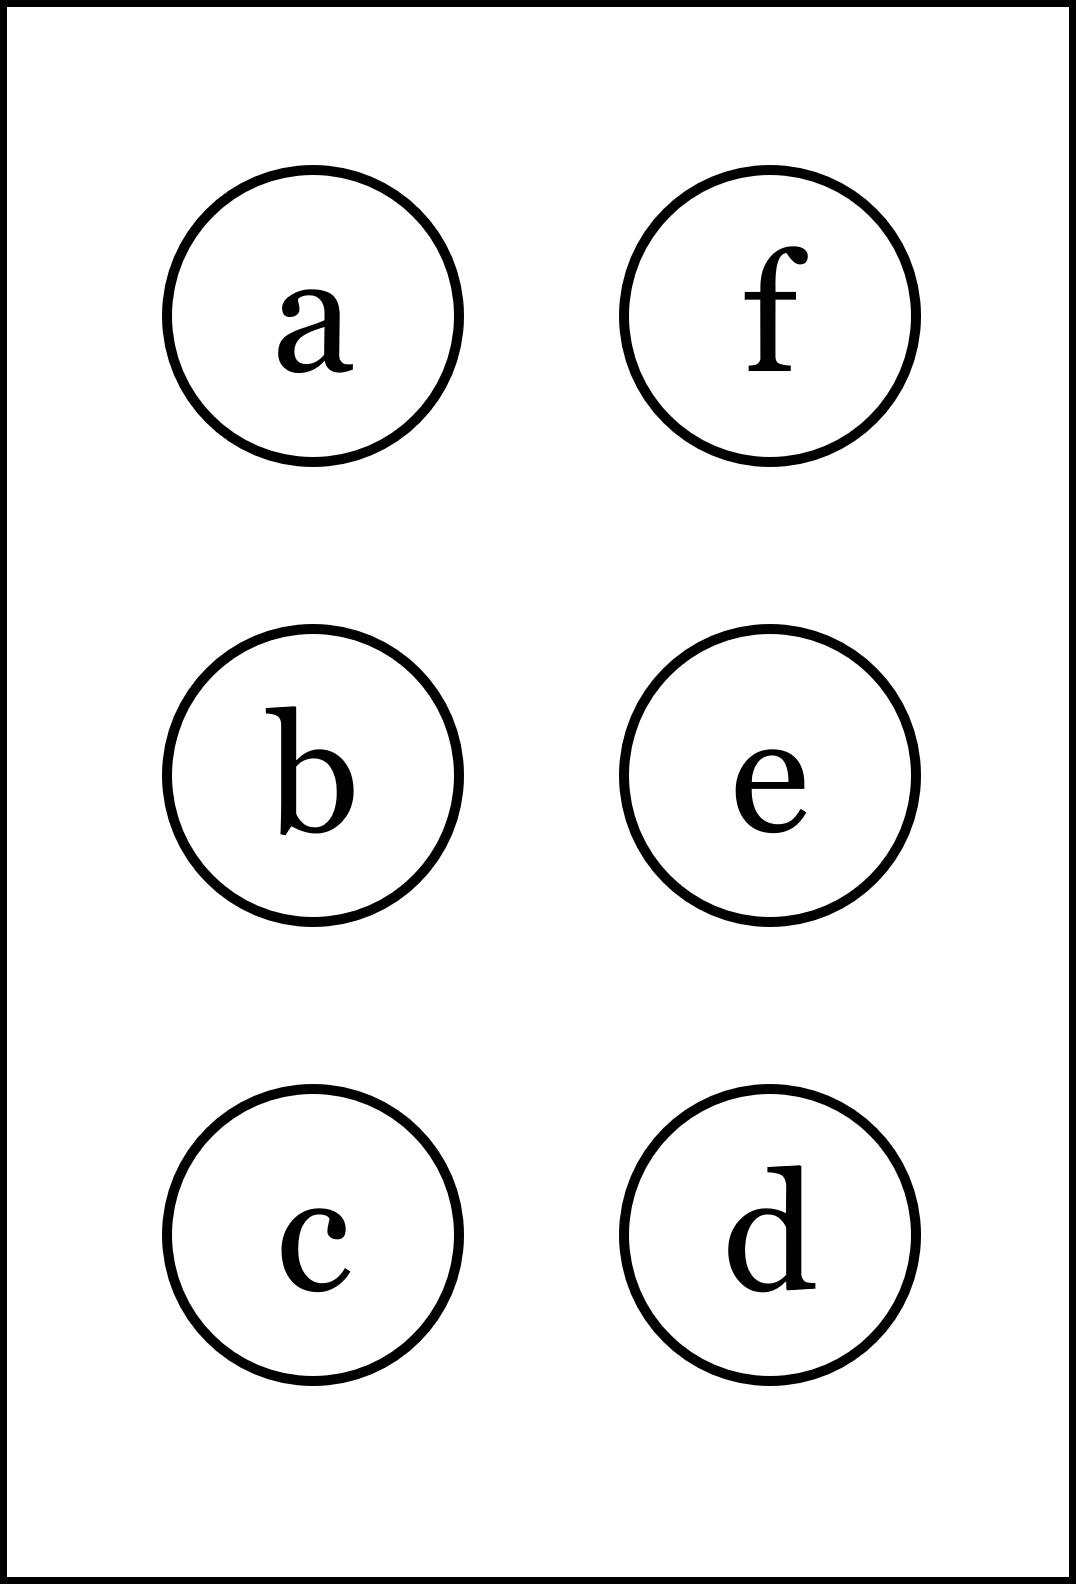
\includegraphics[height=40mm]{../images/braille.png}
{\small Písmeno Braillovej abecedy}
\end{center}
\end{minipage}
\end{center}
\end{minipage}
&
\begin{minipage}[c][104.5mm][t]{0.5\linewidth}
\begin{center}
\vspace{7mm}
{\huge Volné extrémy, skupina \textit{Lambda $\lambda$} -\romannumeral4}\\[5mm]
\textit{Jméno:}\phantom{xxxxxxxxxxxxxxxxxxxxxxxxxxxxxxxxxxxxxxxxxxxxxxxxxxxxxxxxxxxxxxxxx}\\[5mm]
\begin{minipage}{0.95\linewidth}
\begin{center}
Cílem je najít \textbf{volné extrémy} funkce $f(x,y)$ zadané v \textbf{(a)}.\\Postupuj podle krokú v \textbf{(b)} až \textbf{(f)}. Pokud se medzivýsledky shodujú s těmi za otazníky,\\tak napravo obarvi příslušející kroužek načerno. \textbf{Spolu odevzdejte výsledné slovo}.
\end{center}
\end{minipage}
\\[1mm]
\begin{minipage}{0.79\linewidth}
\begin{center}
\begin{varwidth}{\linewidth}
\begin{enumerate}
\normalsize
\item $f(x,y)=3x^3+18x^2-108x+4+9y+3y^2-y^3$\quad \dotfill\; ???\;\dotfill \quad vybarvi
\item Najdi parciální derivaci podle $x$, $\pdv{f}{x}=$\quad \dotfill\; ???\;\dotfill \quad $9x^2+18x-108$
\item Najdi stacionární body v $x$\quad \dotfill\; ???\;\dotfill \quad $x_1+x_2=-3$
\item Najdi parciální derivaci podle $y$, $\pdv{f}{y}=$\quad \dotfill\; ???\;\dotfill \quad $-3y^2+6y+6$
\item Najdi stacionární body v $y$\quad \dotfill\; ???\;\dotfill \quad $y_1+y_2=3$
\item Najdi funkční hodnoty vo všech stacionárních bodech \\ \phantom{xxxxxx} a vyber tu najvětší. $f_{\text{max}}(x,y)=$\quad \dotfill\; ???\;\dotfill \quad $647$
\end{enumerate}
\end{varwidth}
\end{center}
\end{minipage}
\begin{minipage}{0.20\linewidth}
\begin{center}
{\Huge\bfseries 4.} \\[2mm]
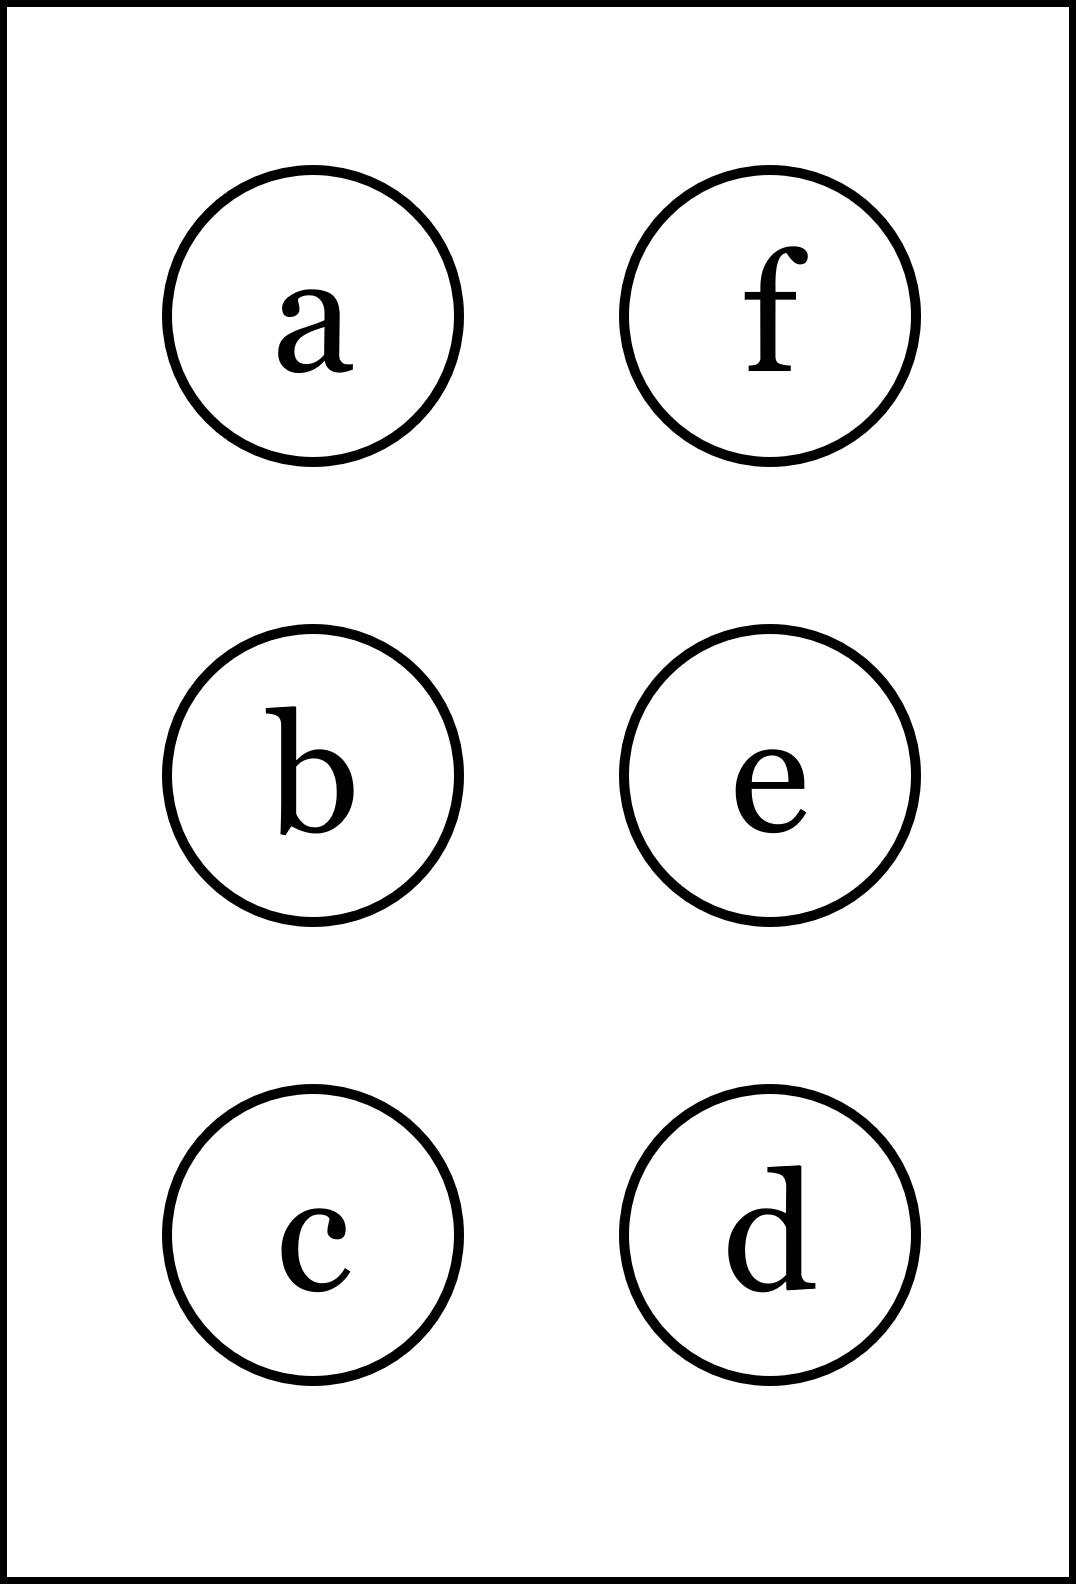
\includegraphics[height=40mm]{../images/braille.png}
{\small Písmeno Braillovej abecedy}
\end{center}
\end{minipage}
\end{center}
\end{minipage}
%
\end{tabular}
\newpage
\thispagestyle{empty}
\begin{tabular}{c:c}
\begin{minipage}[c][104.5mm][t]{0.5\linewidth}
\begin{center}
\vspace{7mm}
{\huge Volné extrémy, skupina \textit{Mu $\mu$} -\romannumeral1}\\[5mm]
\textit{Jméno:}\phantom{xxxxxxxxxxxxxxxxxxxxxxxxxxxxxxxxxxxxxxxxxxxxxxxxxxxxxxxxxxxxxxxxx}\\[5mm]
\begin{minipage}{0.95\linewidth}
\begin{center}
Cílem je najít \textbf{volné extrémy} funkce $f(x,y)$ zadané v \textbf{(a)}.\\Postupuj podle krokú v \textbf{(b)} až \textbf{(f)}. Pokud se medzivýsledky shodujú s těmi za otazníky,\\tak napravo obarvi příslušející kroužek načerno. \textbf{Spolu odevzdejte výsledné slovo}.
\end{center}
\end{minipage}
\\[1mm]
\begin{minipage}{0.79\linewidth}
\begin{center}
\begin{varwidth}{\linewidth}
\begin{enumerate}
\normalsize
\item $f(x,y)=x^3-6x^2-63x-1-60y+24y^2+4y^3$\quad \dotfill\; ???\;\dotfill \quad vybarvi
\item Najdi parciální derivaci podle $x$, $\pdv{f}{x}=$\quad \dotfill\; ???\;\dotfill \quad $3x^2-6x-63$
\item Najdi stacionární body v $x$\quad \dotfill\; ???\;\dotfill \quad $x_1+x_2=5$
\item Najdi parciální derivaci podle $y$, $\pdv{f}{y}=$\quad \dotfill\; ???\;\dotfill \quad $12y^2+48y-36$
\item Najdi stacionární body v $y$\quad \dotfill\; ???\;\dotfill \quad $y_1+y_2=-4$
\item Najdi funkční hodnoty vo všech stacionárních bodech \\ \phantom{xxxxxx} a vyber tu najvětší. $f_{\text{max}}(x,y)=$\quad \dotfill\; ???\;\dotfill \quad $75$
\end{enumerate}
\end{varwidth}
\end{center}
\end{minipage}
\begin{minipage}{0.20\linewidth}
\begin{center}
{\Huge\bfseries 1.} \\[2mm]
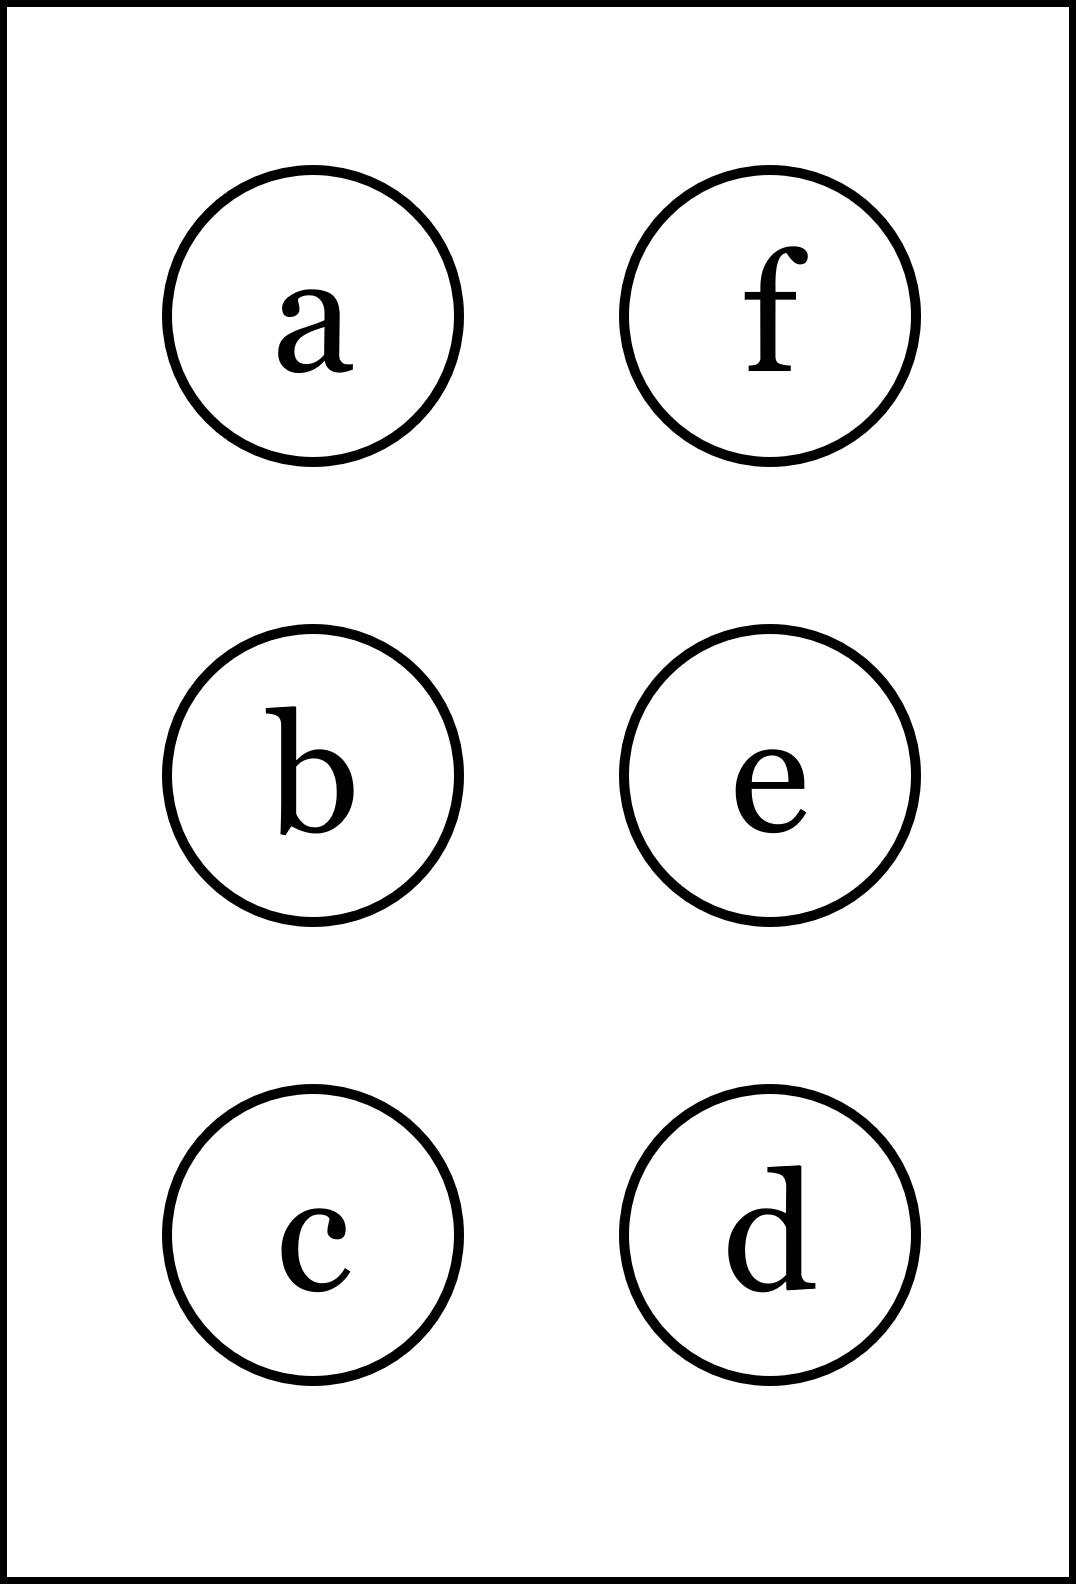
\includegraphics[height=40mm]{../images/braille.png}
{\small Písmeno Braillovej abecedy}
\end{center}
\end{minipage}
\end{center}
\end{minipage}
&
\begin{minipage}[c][104.5mm][t]{0.5\linewidth}
\begin{center}
\vspace{7mm}
{\huge Volné extrémy, skupina \textit{Mu $\mu$} -\romannumeral2}\\[5mm]
\textit{Jméno:}\phantom{xxxxxxxxxxxxxxxxxxxxxxxxxxxxxxxxxxxxxxxxxxxxxxxxxxxxxxxxxxxxxxxxx}\\[5mm]
\begin{minipage}{0.95\linewidth}
\begin{center}
Cílem je najít \textbf{volné extrémy} funkce $f(x,y)$ zadané v \textbf{(a)}.\\Postupuj podle krokú v \textbf{(b)} až \textbf{(f)}. Pokud se medzivýsledky shodujú s těmi za otazníky,\\tak napravo obarvi příslušející kroužek načerno. \textbf{Spolu odevzdejte výsledné slovo}.
\end{center}
\end{minipage}
\\[1mm]
\begin{minipage}{0.79\linewidth}
\begin{center}
\begin{varwidth}{\linewidth}
\begin{enumerate}
\normalsize
\item $f(x,y)=4x^3-12x^2-36x+5-24y-9y^2-y^3$\quad \dotfill\; ???\;\dotfill \quad vybarvi
\item Najdi parciální derivaci podle $x$, $\pdv{f}{x}=$\quad \dotfill\; ???\;\dotfill \quad $12x^2-12x-36$
\item Najdi stacionární body v $x$\quad \dotfill\; ???\;\dotfill \quad $x_1+x_2=2$
\item Najdi parciální derivaci podle $y$, $\pdv{f}{y}=$\quad \dotfill\; ???\;\dotfill \quad $-3y^2-18y-24$
\item Najdi stacionární body v $y$\quad \dotfill\; ???\;\dotfill \quad $y_1+y_2=-5$
\item Najdi funkční hodnoty vo všech stacionárních bodech \\ \phantom{xxxxxx} a vyber tu najvětší. $f_{\text{max}}(x,y)=$\quad \dotfill\; ???\;\dotfill \quad $-87$
\end{enumerate}
\end{varwidth}
\end{center}
\end{minipage}
\begin{minipage}{0.20\linewidth}
\begin{center}
{\Huge\bfseries 2.} \\[2mm]
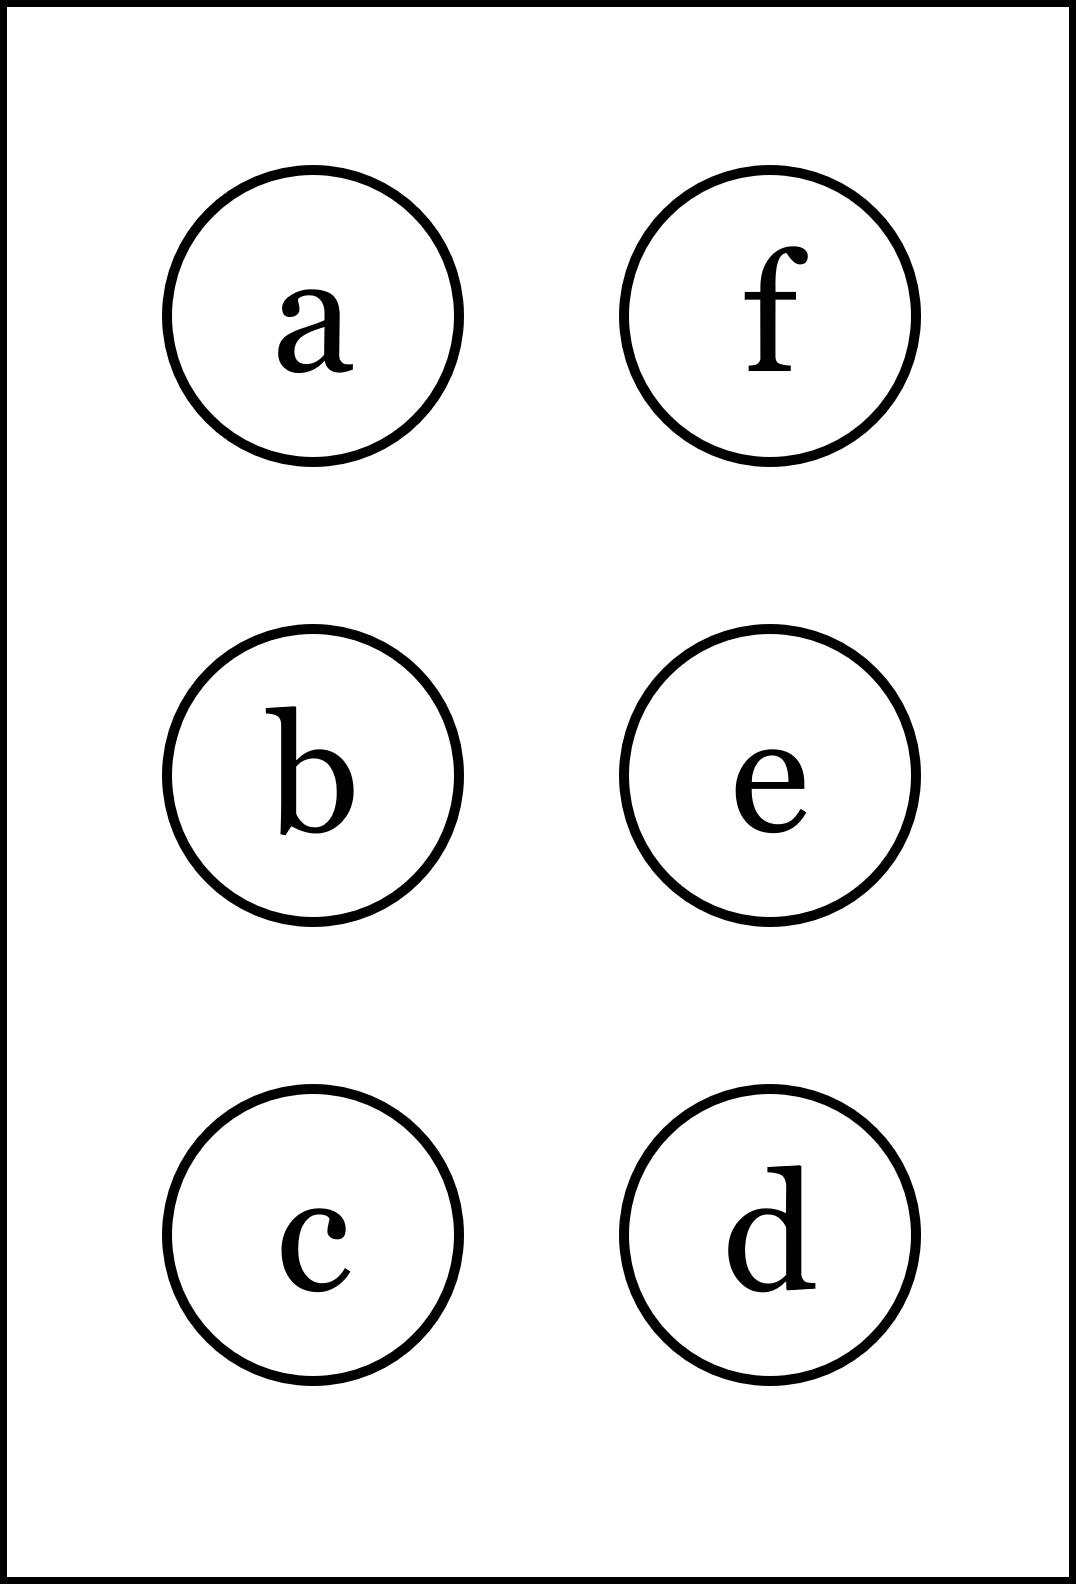
\includegraphics[height=40mm]{../images/braille.png}
{\small Písmeno Braillovej abecedy}
\end{center}
\end{minipage}
\end{center}
\end{minipage}
\\ \hdashline
\begin{minipage}[c][104.5mm][t]{0.5\linewidth}
\begin{center}
\vspace{7mm}
{\huge Volné extrémy, skupina \textit{Mu $\mu$} -\romannumeral3}\\[5mm]
\textit{Jméno:}\phantom{xxxxxxxxxxxxxxxxxxxxxxxxxxxxxxxxxxxxxxxxxxxxxxxxxxxxxxxxxxxxxxxxx}\\[5mm]
\begin{minipage}{0.95\linewidth}
\begin{center}
Cílem je najít \textbf{volné extrémy} funkce $f(x,y)$ zadané v \textbf{(a)}.\\Postupuj podle krokú v \textbf{(b)} až \textbf{(f)}. Pokud se medzivýsledky shodujú s těmi za otazníky,\\tak napravo obarvi příslušející kroužek načerno. \textbf{Spolu odevzdejte výsledné slovo}.
\end{center}
\end{minipage}
\\[1mm]
\begin{minipage}{0.79\linewidth}
\begin{center}
\begin{varwidth}{\linewidth}
\begin{enumerate}
\normalsize
\item $f(x,y)=-6x^3-36x^2+90x+1+9y+3y^2-y^3$\quad \dotfill\; ???\;\dotfill \quad vybarvi
\item Najdi parciální derivaci podle $x$, $\pdv{f}{x}=$\quad \dotfill\; ???\;\dotfill \quad $-18x^2-72x+90$
\item Najdi stacionární body v $x$\quad \dotfill\; ???\;\dotfill \quad $x_1+x_2=-4$
\item Najdi parciální derivaci podle $y$, $\pdv{f}{y}=$\quad \dotfill\; ???\;\dotfill \quad $-3y^2+6y+18$
\item Najdi stacionární body v $y$\quad \dotfill\; ???\;\dotfill \quad $y_1+y_2=2$
\item Najdi funkční hodnoty vo všech stacionárních bodech \\ \phantom{xxxxxx} a vyber tu najvětší. $f_{\text{max}}(x,y)=$\quad \dotfill\; ???\;\dotfill \quad $-604$
\end{enumerate}
\end{varwidth}
\end{center}
\end{minipage}
\begin{minipage}{0.20\linewidth}
\begin{center}
{\Huge\bfseries 3.} \\[2mm]
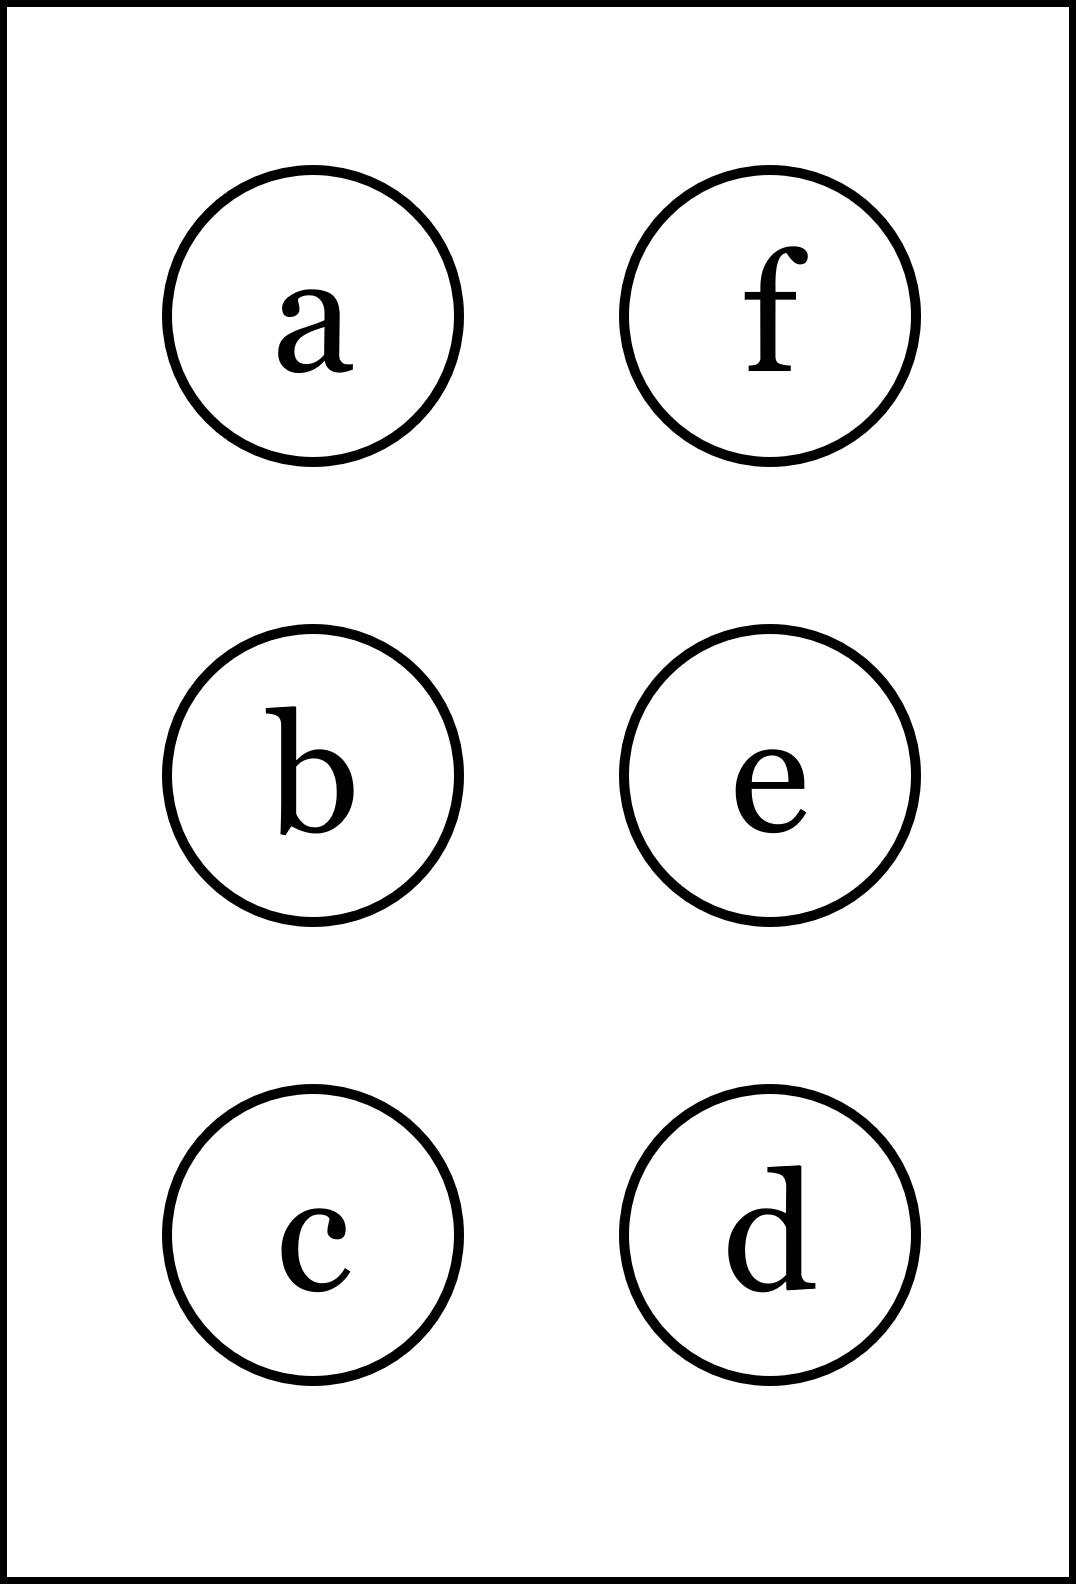
\includegraphics[height=40mm]{../images/braille.png}
{\small Písmeno Braillovej abecedy}
\end{center}
\end{minipage}
\end{center}
\end{minipage}
&
\begin{minipage}[c][104.5mm][t]{0.5\linewidth}
\begin{center}
\vspace{7mm}
{\huge Volné extrémy, skupina \textit{Mu $\mu$} -\romannumeral4}\\[5mm]
\textit{Jméno:}\phantom{xxxxxxxxxxxxxxxxxxxxxxxxxxxxxxxxxxxxxxxxxxxxxxxxxxxxxxxxxxxxxxxxx}\\[5mm]
\begin{minipage}{0.95\linewidth}
\begin{center}
Cílem je najít \textbf{volné extrémy} funkce $f(x,y)$ zadané v \textbf{(a)}.\\Postupuj podle krokú v \textbf{(b)} až \textbf{(f)}. Pokud se medzivýsledky shodujú s těmi za otazníky,\\tak napravo obarvi příslušející kroužek načerno. \textbf{Spolu odevzdejte výsledné slovo}.
\end{center}
\end{minipage}
\\[1mm]
\begin{minipage}{0.79\linewidth}
\begin{center}
\begin{varwidth}{\linewidth}
\begin{enumerate}
\normalsize
\item $f(x,y)=x^3+6x^2-36x+4-60y+24y^2+4y^3$\quad \dotfill\; ???\;\dotfill \quad vybarvi
\item Najdi parciální derivaci podle $x$, $\pdv{f}{x}=$\quad \dotfill\; ???\;\dotfill \quad $3x^2+6x-36$
\item Najdi stacionární body v $x$\quad \dotfill\; ???\;\dotfill \quad $x_1+x_2=-4$
\item Najdi parciální derivaci podle $y$, $\pdv{f}{y}=$\quad \dotfill\; ???\;\dotfill \quad $12y^2+48y-36$
\item Najdi stacionární body v $y$\quad \dotfill\; ???\;\dotfill \quad $y_1+y_2=-4$
\item Najdi funkční hodnoty vo všech stacionárních bodech \\ \phantom{xxxxxx} a vyber tu najvětší. $f_{\text{max}}(x,y)=$\quad \dotfill\; ???\;\dotfill \quad $188$
\end{enumerate}
\end{varwidth}
\end{center}
\end{minipage}
\begin{minipage}{0.20\linewidth}
\begin{center}
{\Huge\bfseries 4.} \\[2mm]
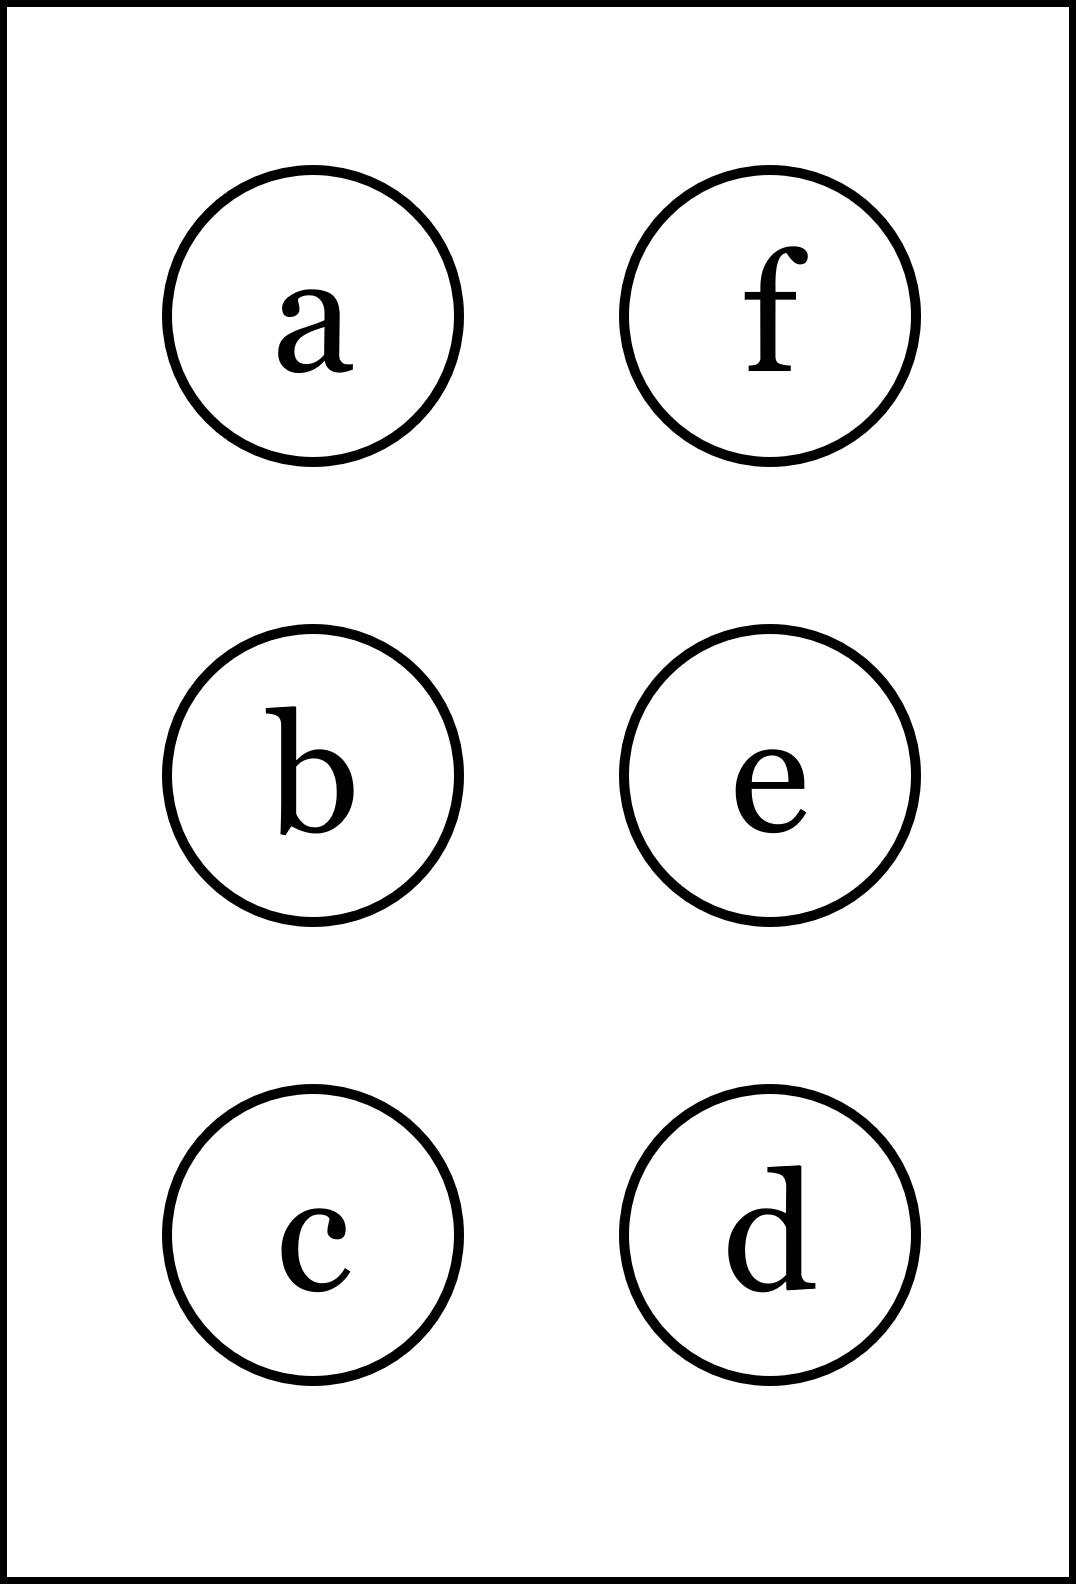
\includegraphics[height=40mm]{../images/braille.png}
{\small Písmeno Braillovej abecedy}
\end{center}
\end{minipage}
\end{center}
\end{minipage}
%
\end{tabular}
\newpage
\thispagestyle{empty}
\begin{tabular}{c:c}
\begin{minipage}[c][104.5mm][t]{0.5\linewidth}
\begin{center}
\vspace{7mm}
{\huge Volné extrémy, skupina \textit{Nu $\nu$} -\romannumeral1}\\[5mm]
\textit{Jméno:}\phantom{xxxxxxxxxxxxxxxxxxxxxxxxxxxxxxxxxxxxxxxxxxxxxxxxxxxxxxxxxxxxxxxxx}\\[5mm]
\begin{minipage}{0.95\linewidth}
\begin{center}
Cílem je najít \textbf{volné extrémy} funkce $f(x,y)$ zadané v \textbf{(a)}.\\Postupuj podle krokú v \textbf{(b)} až \textbf{(f)}. Pokud se medzivýsledky shodujú s těmi za otazníky,\\tak napravo obarvi příslušející kroužek načerno. \textbf{Spolu odevzdejte výsledné slovo}.
\end{center}
\end{minipage}
\\[1mm]
\begin{minipage}{0.79\linewidth}
\begin{center}
\begin{varwidth}{\linewidth}
\begin{enumerate}
\normalsize
\item $f(x,y)=3x^3+18x^2-45x-2+180y-30y^2-5y^3$\quad \dotfill\; ???\;\dotfill \quad vybarvi
\item Najdi parciální derivaci podle $x$, $\pdv{f}{x}=$\quad \dotfill\; ???\;\dotfill \quad $9x^2+18x-45$
\item Najdi stacionární body v $x$\quad \dotfill\; ???\;\dotfill \quad $x_1+x_2=-4$
\item Najdi parciální derivaci podle $y$, $\pdv{f}{y}=$\quad \dotfill\; ???\;\dotfill \quad $-15y^2-60y+120$
\item Najdi stacionární body v $y$\quad \dotfill\; ???\;\dotfill \quad $y_1+y_2=-4$
\item Najdi funkční hodnoty vo všech stacionárních bodech \\ \phantom{xxxxxx} a vyber tu najvětší. $f_{\text{max}}(x,y)=$\quad \dotfill\; ???\;\dotfill \quad $-1106$
\end{enumerate}
\end{varwidth}
\end{center}
\end{minipage}
\begin{minipage}{0.20\linewidth}
\begin{center}
{\Huge\bfseries 1.} \\[2mm]
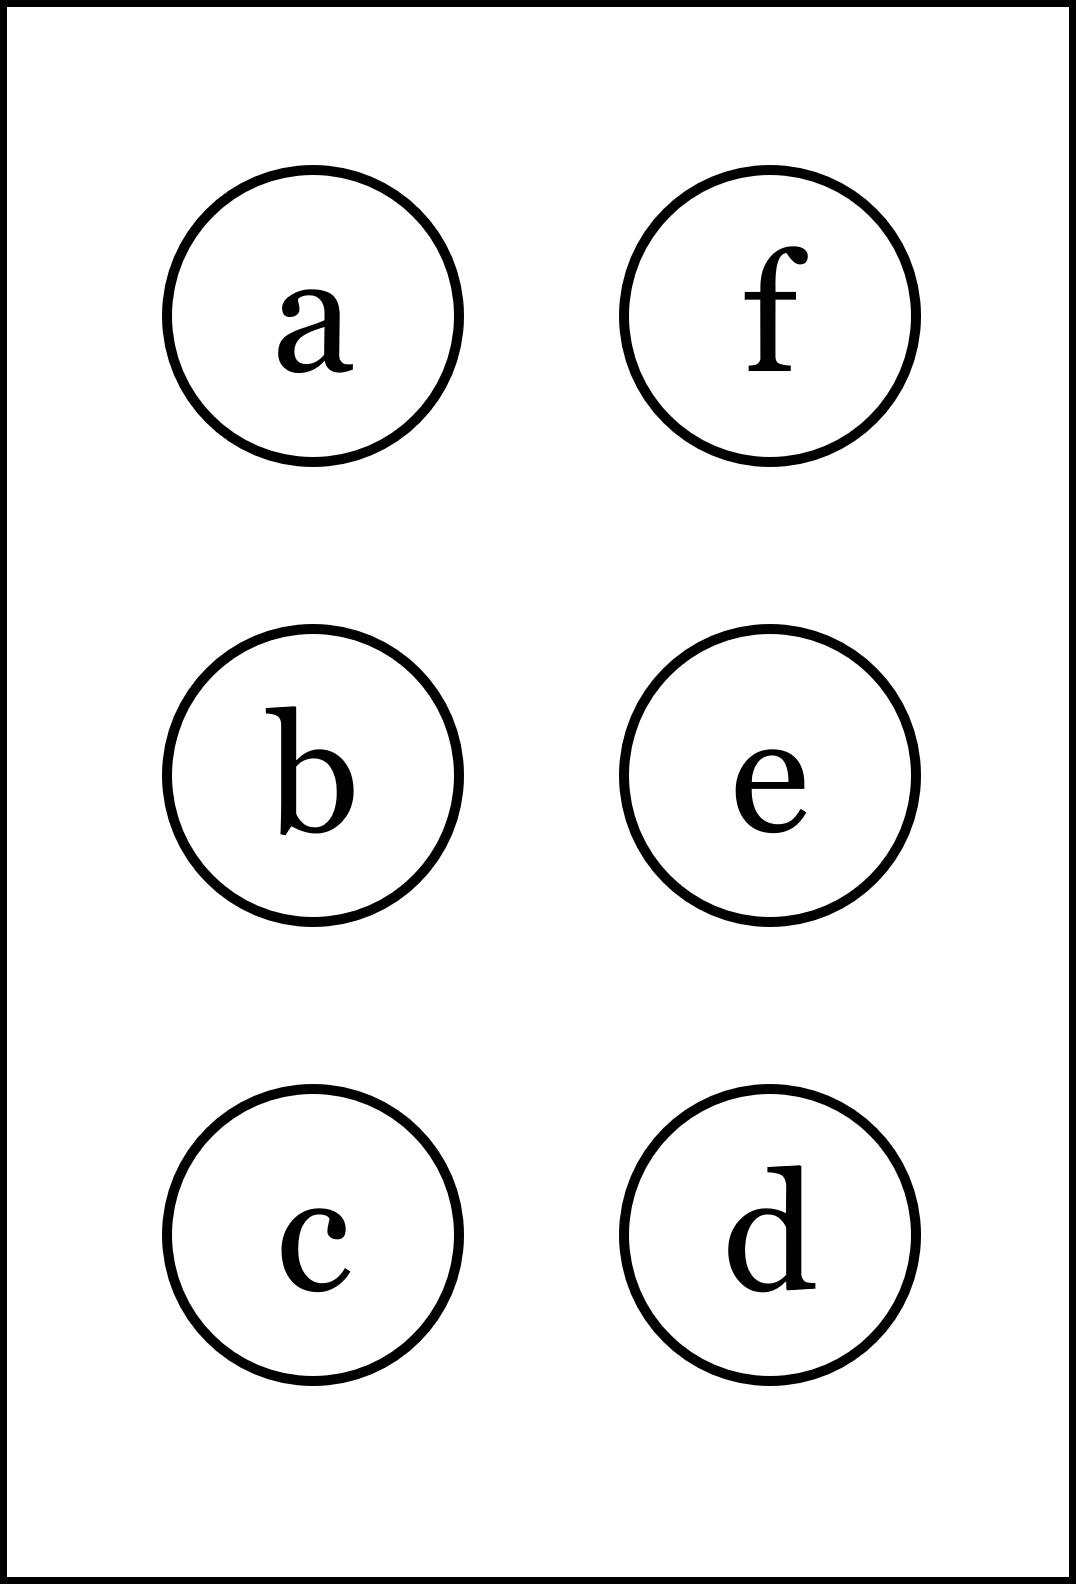
\includegraphics[height=40mm]{../images/braille.png}
{\small Písmeno Braillovej abecedy}
\end{center}
\end{minipage}
\end{center}
\end{minipage}
&
\begin{minipage}[c][104.5mm][t]{0.5\linewidth}
\begin{center}
\vspace{7mm}
{\huge Volné extrémy, skupina \textit{Nu $\nu$} -\romannumeral2}\\[5mm]
\textit{Jméno:}\phantom{xxxxxxxxxxxxxxxxxxxxxxxxxxxxxxxxxxxxxxxxxxxxxxxxxxxxxxxxxxxxxxxxx}\\[5mm]
\begin{minipage}{0.95\linewidth}
\begin{center}
Cílem je najít \textbf{volné extrémy} funkce $f(x,y)$ zadané v \textbf{(a)}.\\Postupuj podle krokú v \textbf{(b)} až \textbf{(f)}. Pokud se medzivýsledky shodujú s těmi za otazníky,\\tak napravo obarvi příslušející kroužek načerno. \textbf{Spolu odevzdejte výsledné slovo}.
\end{center}
\end{minipage}
\\[1mm]
\begin{minipage}{0.79\linewidth}
\begin{center}
\begin{varwidth}{\linewidth}
\begin{enumerate}
\normalsize
\item $f(x,y)=-x^3-6x^2+15x+2-18y+6y^2+2y^3$\quad \dotfill\; ???\;\dotfill \quad vybarvi
\item Najdi parciální derivaci podle $x$, $\pdv{f}{x}=$\quad \dotfill\; ???\;\dotfill \quad $-3x^2-6x+15$
\item Najdi stacionární body v $x$\quad \dotfill\; ???\;\dotfill \quad $x_1+x_2=-4$
\item Najdi parciální derivaci podle $y$, $\pdv{f}{y}=$\quad \dotfill\; ???\;\dotfill \quad $6y^2+12y-12$
\item Najdi stacionární body v $y$\quad \dotfill\; ???\;\dotfill \quad $y_1+y_2=-1$
\item Najdi funkční hodnoty vo všech stacionárních bodech \\ \phantom{xxxxxx} a vyber tu najvětší. $f_{\text{max}}(x,y)=$\quad \dotfill\; ???\;\dotfill \quad $0$
\end{enumerate}
\end{varwidth}
\end{center}
\end{minipage}
\begin{minipage}{0.20\linewidth}
\begin{center}
{\Huge\bfseries 2.} \\[2mm]
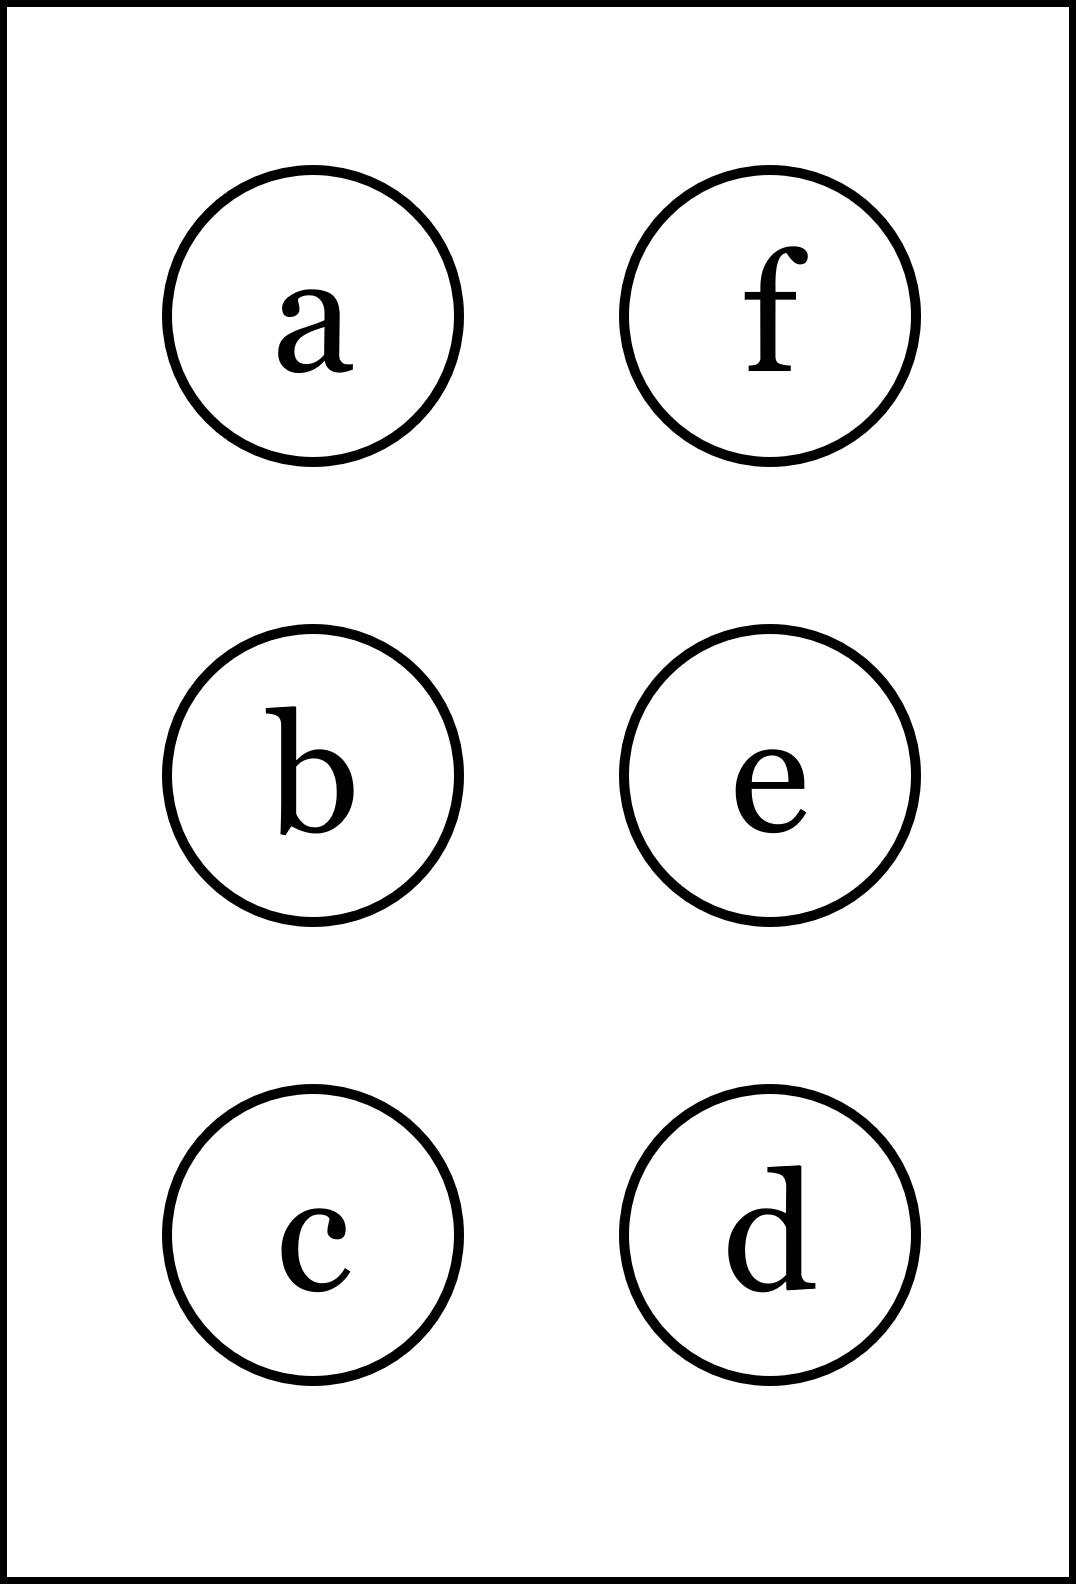
\includegraphics[height=40mm]{../images/braille.png}
{\small Písmeno Braillovej abecedy}
\end{center}
\end{minipage}
\end{center}
\end{minipage}
\\ \hdashline
\begin{minipage}[c][104.5mm][t]{0.5\linewidth}
\begin{center}
\vspace{7mm}
{\huge Volné extrémy, skupina \textit{Nu $\nu$} -\romannumeral3}\\[5mm]
\textit{Jméno:}\phantom{xxxxxxxxxxxxxxxxxxxxxxxxxxxxxxxxxxxxxxxxxxxxxxxxxxxxxxxxxxxxxxxxx}\\[5mm]
\begin{minipage}{0.95\linewidth}
\begin{center}
Cílem je najít \textbf{volné extrémy} funkce $f(x,y)$ zadané v \textbf{(a)}.\\Postupuj podle krokú v \textbf{(b)} až \textbf{(f)}. Pokud se medzivýsledky shodujú s těmi za otazníky,\\tak napravo obarvi příslušející kroužek načerno. \textbf{Spolu odevzdejte výsledné slovo}.
\end{center}
\end{minipage}
\\[1mm]
\begin{minipage}{0.79\linewidth}
\begin{center}
\begin{varwidth}{\linewidth}
\begin{enumerate}
\normalsize
\item $f(x,y)=2x^3-12x^2-30x-4-48y-9y^2+y^3$\quad \dotfill\; ???\;\dotfill \quad vybarvi
\item Najdi parciální derivaci podle $x$, $\pdv{f}{x}=$\quad \dotfill\; ???\;\dotfill \quad $6x^2-12x-30$
\item Najdi stacionární body v $x$\quad \dotfill\; ???\;\dotfill \quad $x_1+x_2=4$
\item Najdi parciální derivaci podle $y$, $\pdv{f}{y}=$\quad \dotfill\; ???\;\dotfill \quad $3y^2-18y-30$
\item Najdi stacionární body v $y$\quad \dotfill\; ???\;\dotfill \quad $y_1+y_2=6$
\item Najdi funkční hodnoty vo všech stacionárních bodech \\ \phantom{xxxxxx} a vyber tu najvětší. $f_{\text{max}}(x,y)=$\quad \dotfill\; ???\;\dotfill \quad $64$
\end{enumerate}
\end{varwidth}
\end{center}
\end{minipage}
\begin{minipage}{0.20\linewidth}
\begin{center}
{\Huge\bfseries 3.} \\[2mm]
\includegraphics[height=40mm]{../images/braille.png}
{\small Písmeno Braillovej abecedy}
\end{center}
\end{minipage}
\end{center}
\end{minipage}
&
\begin{minipage}[c][104.5mm][t]{0.5\linewidth}
\begin{center}
\vspace{7mm}
{\huge Volné extrémy, skupina \textit{Nu $\nu$} -\romannumeral4}\\[5mm]
\textit{Jméno:}\phantom{xxxxxxxxxxxxxxxxxxxxxxxxxxxxxxxxxxxxxxxxxxxxxxxxxxxxxxxxxxxxxxxxx}\\[5mm]
\begin{minipage}{0.95\linewidth}
\begin{center}
Cílem je najít \textbf{volné extrémy} funkce $f(x,y)$ zadané v \textbf{(a)}.\\Postupuj podle krokú v \textbf{(b)} až \textbf{(f)}. Pokud se medzivýsledky shodujú s těmi za otazníky,\\tak napravo obarvi příslušející kroužek načerno. \textbf{Spolu odevzdejte výsledné slovo}.
\end{center}
\end{minipage}
\\[1mm]
\begin{minipage}{0.79\linewidth}
\begin{center}
\begin{varwidth}{\linewidth}
\begin{enumerate}
\normalsize
\item $f(x,y)=-x^3+6x^2+36x+3+9y+6y^2+y^3$\quad \dotfill\; ???\;\dotfill \quad vybarvi
\item Najdi parciální derivaci podle $x$, $\pdv{f}{x}=$\quad \dotfill\; ???\;\dotfill \quad $-3x^2+6x+36$
\item Najdi stacionární body v $x$\quad \dotfill\; ???\;\dotfill \quad $x_1+x_2=4$
\item Najdi parciální derivaci podle $y$, $\pdv{f}{y}=$\quad \dotfill\; ???\;\dotfill \quad $3y^2+12y-9$
\item Najdi stacionární body v $y$\quad \dotfill\; ???\;\dotfill \quad $y_1+y_2=-4$
\item Najdi funkční hodnoty vo všech stacionárních bodech \\ \phantom{xxxxxx} a vyber tu najvětší. $f_{\text{max}}(x,y)=$\quad \dotfill\; ???\;\dotfill \quad $-41$
\end{enumerate}
\end{varwidth}
\end{center}
\end{minipage}
\begin{minipage}{0.20\linewidth}
\begin{center}
{\Huge\bfseries 4.} \\[2mm]
\includegraphics[height=40mm]{../images/braille.png}
{\small Písmeno Braillovej abecedy}
\end{center}
\end{minipage}
\end{center}
\end{minipage}
%
\end{tabular}
\newpage
\thispagestyle{empty}
\begin{tabular}{c:c}
\begin{minipage}[c][104.5mm][t]{0.5\linewidth}
\begin{center}
\vspace{7mm}
{\huge Volné extrémy, skupina \textit{Xi $\xi$} -\romannumeral1}\\[5mm]
\textit{Jméno:}\phantom{xxxxxxxxxxxxxxxxxxxxxxxxxxxxxxxxxxxxxxxxxxxxxxxxxxxxxxxxxxxxxxxxx}\\[5mm]
\begin{minipage}{0.95\linewidth}
\begin{center}
Cílem je najít \textbf{volné extrémy} funkce $f(x,y)$ zadané v \textbf{(a)}.\\Postupuj podle krokú v \textbf{(b)} až \textbf{(f)}. Pokud se medzivýsledky shodujú s těmi za otazníky,\\tak napravo obarvi příslušející kroužek načerno. \textbf{Spolu odevzdejte výsledné slovo}.
\end{center}
\end{minipage}
\\[1mm]
\begin{minipage}{0.79\linewidth}
\begin{center}
\begin{varwidth}{\linewidth}
\begin{enumerate}
\normalsize
\item $f(x,y)=x^3+6x^2-15x+5+108y+18y^2-3y^3$\quad \dotfill\; ???\;\dotfill \quad vybarvi
\item Najdi parciální derivaci podle $x$, $\pdv{f}{x}=$\quad \dotfill\; ???\;\dotfill \quad $3x^2+12x-15$
\item Najdi stacionární body v $x$\quad \dotfill\; ???\;\dotfill \quad $x_1+x_2=-4$
\item Najdi parciální derivaci podle $y$, $\pdv{f}{y}=$\quad \dotfill\; ???\;\dotfill \quad $-9y^2+36y+72$
\item Najdi stacionární body v $y$\quad \dotfill\; ???\;\dotfill \quad $y_1+y_2=5$
\item Najdi funkční hodnoty vo všech stacionárních bodech \\ \phantom{xxxxxx} a vyber tu najvětší. $f_{\text{max}}(x,y)=$\quad \dotfill\; ???\;\dotfill \quad $-15$
\end{enumerate}
\end{varwidth}
\end{center}
\end{minipage}
\begin{minipage}{0.20\linewidth}
\begin{center}
{\Huge\bfseries 1.} \\[2mm]
\includegraphics[height=40mm]{../images/braille.png}
{\small Písmeno Braillovej abecedy}
\end{center}
\end{minipage}
\end{center}
\end{minipage}
&
\begin{minipage}[c][104.5mm][t]{0.5\linewidth}
\begin{center}
\vspace{7mm}
{\huge Volné extrémy, skupina \textit{Xi $\xi$} -\romannumeral2}\\[5mm]
\textit{Jméno:}\phantom{xxxxxxxxxxxxxxxxxxxxxxxxxxxxxxxxxxxxxxxxxxxxxxxxxxxxxxxxxxxxxxxxx}\\[5mm]
\begin{minipage}{0.95\linewidth}
\begin{center}
Cílem je najít \textbf{volné extrémy} funkce $f(x,y)$ zadané v \textbf{(a)}.\\Postupuj podle krokú v \textbf{(b)} až \textbf{(f)}. Pokud se medzivýsledky shodujú s těmi za otazníky,\\tak napravo obarvi příslušející kroužek načerno. \textbf{Spolu odevzdejte výsledné slovo}.
\end{center}
\end{minipage}
\\[1mm]
\begin{minipage}{0.79\linewidth}
\begin{center}
\begin{varwidth}{\linewidth}
\begin{enumerate}
\normalsize
\item $f(x,y)=2x^3+6x^2-18x+1-108y+18y^2+3y^3$\quad \dotfill\; ???\;\dotfill \quad vybarvi
\item Najdi parciální derivaci podle $x$, $\pdv{f}{x}=$\quad \dotfill\; ???\;\dotfill \quad $6x^2+6x-18$
\item Najdi stacionární body v $x$\quad \dotfill\; ???\;\dotfill \quad $x_1+x_2=-1$
\item Najdi parciální derivaci podle $y$, $\pdv{f}{y}=$\quad \dotfill\; ???\;\dotfill \quad $9y^2+36y-72$
\item Najdi stacionární body v $y$\quad \dotfill\; ???\;\dotfill \quad $y_1+y_2=-3$
\item Najdi funkční hodnoty vo všech stacionárních bodech \\ \phantom{xxxxxx} a vyber tu najvětší. $f_{\text{max}}(x,y)=$\quad \dotfill\; ???\;\dotfill \quad $-65$
\end{enumerate}
\end{varwidth}
\end{center}
\end{minipage}
\begin{minipage}{0.20\linewidth}
\begin{center}
{\Huge\bfseries 2.} \\[2mm]
\includegraphics[height=40mm]{../images/braille.png}
{\small Písmeno Braillovej abecedy}
\end{center}
\end{minipage}
\end{center}
\end{minipage}
\\ \hdashline
\begin{minipage}[c][104.5mm][t]{0.5\linewidth}
\begin{center}
\vspace{7mm}
{\huge Volné extrémy, skupina \textit{Xi $\xi$} -\romannumeral3}\\[5mm]
\textit{Jméno:}\phantom{xxxxxxxxxxxxxxxxxxxxxxxxxxxxxxxxxxxxxxxxxxxxxxxxxxxxxxxxxxxxxxxxx}\\[5mm]
\begin{minipage}{0.95\linewidth}
\begin{center}
Cílem je najít \textbf{volné extrémy} funkce $f(x,y)$ zadané v \textbf{(a)}.\\Postupuj podle krokú v \textbf{(b)} až \textbf{(f)}. Pokud se medzivýsledky shodujú s těmi za otazníky,\\tak napravo obarvi příslušející kroužek načerno. \textbf{Spolu odevzdejte výsledné slovo}.
\end{center}
\end{minipage}
\\[1mm]
\begin{minipage}{0.79\linewidth}
\begin{center}
\begin{varwidth}{\linewidth}
\begin{enumerate}
\normalsize
\item $f(x,y)=-x^3-6x^2+15x+7+48y-6y^2-2y^3$\quad \dotfill\; ???\;\dotfill \quad vybarvi
\item Najdi parciální derivaci podle $x$, $\pdv{f}{x}=$\quad \dotfill\; ???\;\dotfill \quad $-3x^2-6x+15$
\item Najdi stacionární body v $x$\quad \dotfill\; ???\;\dotfill \quad $x_1+x_2=-4$
\item Najdi parciální derivaci podle $y$, $\pdv{f}{y}=$\quad \dotfill\; ???\;\dotfill \quad $-6y^2-12y+36$
\item Najdi stacionární body v $y$\quad \dotfill\; ???\;\dotfill \quad $y_1+y_2=-2$
\item Najdi funkční hodnoty vo všech stacionárních bodech \\ \phantom{xxxxxx} a vyber tu najvětší. $f_{\text{max}}(x,y)=$\quad \dotfill\; ???\;\dotfill \quad $71$
\end{enumerate}
\end{varwidth}
\end{center}
\end{minipage}
\begin{minipage}{0.20\linewidth}
\begin{center}
{\Huge\bfseries 3.} \\[2mm]
\includegraphics[height=40mm]{../images/braille.png}
{\small Písmeno Braillovej abecedy}
\end{center}
\end{minipage}
\end{center}
\end{minipage}
&
\begin{minipage}[c][104.5mm][t]{0.5\linewidth}
\begin{center}
\vspace{7mm}
{\huge Volné extrémy, skupina \textit{Xi $\xi$} -\romannumeral4}\\[5mm]
\textit{Jméno:}\phantom{xxxxxxxxxxxxxxxxxxxxxxxxxxxxxxxxxxxxxxxxxxxxxxxxxxxxxxxxxxxxxxxxx}\\[5mm]
\begin{minipage}{0.95\linewidth}
\begin{center}
Cílem je najít \textbf{volné extrémy} funkce $f(x,y)$ zadané v \textbf{(a)}.\\Postupuj podle krokú v \textbf{(b)} až \textbf{(f)}. Pokud se medzivýsledky shodujú s těmi za otazníky,\\tak napravo obarvi příslušející kroužek načerno. \textbf{Spolu odevzdejte výsledné slovo}.
\end{center}
\end{minipage}
\\[1mm]
\begin{minipage}{0.79\linewidth}
\begin{center}
\begin{varwidth}{\linewidth}
\begin{enumerate}
\normalsize
\item $f(x,y)=x^3-6x^2+9x+1-18y-6y^2+2y^3$\quad \dotfill\; ???\;\dotfill \quad vybarvi
\item Najdi parciální derivaci podle $x$, $\pdv{f}{x}=$\quad \dotfill\; ???\;\dotfill \quad $3x^2-6x+9$
\item Najdi stacionární body v $x$\quad \dotfill\; ???\;\dotfill \quad $x_1+x_2=4$
\item Najdi parciální derivaci podle $y$, $\pdv{f}{y}=$\quad \dotfill\; ???\;\dotfill \quad $6y^2-12y-12$
\item Najdi stacionární body v $y$\quad \dotfill\; ???\;\dotfill \quad $y_1+y_2=2$
\item Najdi funkční hodnoty vo všech stacionárních bodech \\ \phantom{xxxxxx} a vyber tu najvětší. $f_{\text{max}}(x,y)=$\quad \dotfill\; ???\;\dotfill \quad $-53$
\end{enumerate}
\end{varwidth}
\end{center}
\end{minipage}
\begin{minipage}{0.20\linewidth}
\begin{center}
{\Huge\bfseries 4.} \\[2mm]
\includegraphics[height=40mm]{../images/braille.png}
{\small Písmeno Braillovej abecedy}
\end{center}
\end{minipage}
\end{center}
\end{minipage}
%
\end{tabular}
\newpage
\thispagestyle{empty}
\begin{tabular}{c:c}
\begin{minipage}[c][104.5mm][t]{0.5\linewidth}
\begin{center}
\vspace{7mm}
{\huge Volné extrémy, skupina \textit{Omicron $\omicron$} -\romannumeral1}\\[5mm]
\textit{Jméno:}\phantom{xxxxxxxxxxxxxxxxxxxxxxxxxxxxxxxxxxxxxxxxxxxxxxxxxxxxxxxxxxxxxxxxx}\\[5mm]
\begin{minipage}{0.95\linewidth}
\begin{center}
Cílem je najít \textbf{volné extrémy} funkce $f(x,y)$ zadané v \textbf{(a)}.\\Postupuj podle krokú v \textbf{(b)} až \textbf{(f)}. Pokud se medzivýsledky shodujú s těmi za otazníky,\\tak napravo obarvi příslušející kroužek načerno. \textbf{Spolu odevzdejte výsledné slovo}.
\end{center}
\end{minipage}
\\[1mm]
\begin{minipage}{0.79\linewidth}
\begin{center}
\begin{varwidth}{\linewidth}
\begin{enumerate}
\normalsize
\item $f(x,y)=x^3+3x^2-9x-1-15y+6y^2+y^3$\quad \dotfill\; ???\;\dotfill \quad vybarvi
\item Najdi parciální derivaci podle $x$, $\pdv{f}{x}=$\quad \dotfill\; ???\;\dotfill \quad $3x^2+3x-9$
\item Najdi stacionární body v $x$\quad \dotfill\; ???\;\dotfill \quad $x_1+x_2=-2$
\item Najdi parciální derivaci podle $y$, $\pdv{f}{y}=$\quad \dotfill\; ???\;\dotfill \quad $3y^2+12y-9$
\item Najdi stacionární body v $y$\quad \dotfill\; ???\;\dotfill \quad $y_1+y_2=-4$
\item Najdi funkční hodnoty vo všech stacionárních bodech \\ \phantom{xxxxxx} a vyber tu najvětší. $f_{\text{max}}(x,y)=$\quad \dotfill\; ???\;\dotfill \quad $126$
\end{enumerate}
\end{varwidth}
\end{center}
\end{minipage}
\begin{minipage}{0.20\linewidth}
\begin{center}
{\Huge\bfseries 1.} \\[2mm]
\includegraphics[height=40mm]{../images/braille.png}
{\small Písmeno Braillovej abecedy}
\end{center}
\end{minipage}
\end{center}
\end{minipage}
&
\begin{minipage}[c][104.5mm][t]{0.5\linewidth}
\begin{center}
\vspace{7mm}
{\huge Volné extrémy, skupina \textit{Omicron $\omicron$} -\romannumeral2}\\[5mm]
\textit{Jméno:}\phantom{xxxxxxxxxxxxxxxxxxxxxxxxxxxxxxxxxxxxxxxxxxxxxxxxxxxxxxxxxxxxxxxxx}\\[5mm]
\begin{minipage}{0.95\linewidth}
\begin{center}
Cílem je najít \textbf{volné extrémy} funkce $f(x,y)$ zadané v \textbf{(a)}.\\Postupuj podle krokú v \textbf{(b)} až \textbf{(f)}. Pokud se medzivýsledky shodujú s těmi za otazníky,\\tak napravo obarvi příslušející kroužek načerno. \textbf{Spolu odevzdejte výsledné slovo}.
\end{center}
\end{minipage}
\\[1mm]
\begin{minipage}{0.79\linewidth}
\begin{center}
\begin{varwidth}{\linewidth}
\begin{enumerate}
\normalsize
\item $f(x,y)=2x^3-6x^2-18x-3-21y+9y^2+y^3$\quad \dotfill\; ???\;\dotfill \quad vybarvi
\item Najdi parciální derivaci podle $x$, $\pdv{f}{x}=$\quad \dotfill\; ???\;\dotfill \quad $6x^2-6x-18$
\item Najdi stacionární body v $x$\quad \dotfill\; ???\;\dotfill \quad $x_1+x_2=2$
\item Najdi parciální derivaci podle $y$, $\pdv{f}{y}=$\quad \dotfill\; ???\;\dotfill \quad $3y^2+18y-12$
\item Najdi stacionární body v $y$\quad \dotfill\; ???\;\dotfill \quad $y_1+y_2=-6$
\item Najdi funkční hodnoty vo všech stacionárních bodech \\ \phantom{xxxxxx} a vyber tu najvětší. $f_{\text{max}}(x,y)=$\quad \dotfill\; ???\;\dotfill \quad $-4$
\end{enumerate}
\end{varwidth}
\end{center}
\end{minipage}
\begin{minipage}{0.20\linewidth}
\begin{center}
{\Huge\bfseries 2.} \\[2mm]
\includegraphics[height=40mm]{../images/braille.png}
{\small Písmeno Braillovej abecedy}
\end{center}
\end{minipage}
\end{center}
\end{minipage}
\\ \hdashline
\begin{minipage}[c][104.5mm][t]{0.5\linewidth}
\begin{center}
\vspace{7mm}
{\huge Volné extrémy, skupina \textit{Omicron $\omicron$} -\romannumeral3}\\[5mm]
\textit{Jméno:}\phantom{xxxxxxxxxxxxxxxxxxxxxxxxxxxxxxxxxxxxxxxxxxxxxxxxxxxxxxxxxxxxxxxxx}\\[5mm]
\begin{minipage}{0.95\linewidth}
\begin{center}
Cílem je najít \textbf{volné extrémy} funkce $f(x,y)$ zadané v \textbf{(a)}.\\Postupuj podle krokú v \textbf{(b)} až \textbf{(f)}. Pokud se medzivýsledky shodujú s těmi za otazníky,\\tak napravo obarvi příslušející kroužek načerno. \textbf{Spolu odevzdejte výsledné slovo}.
\end{center}
\end{minipage}
\\[1mm]
\begin{minipage}{0.79\linewidth}
\begin{center}
\begin{varwidth}{\linewidth}
\begin{enumerate}
\normalsize
\item $f(x,y)=-6x^3+36x^2-54x+3+45y-3y^2-y^3$\quad \dotfill\; ???\;\dotfill \quad vybarvi
\item Najdi parciální derivaci podle $x$, $\pdv{f}{x}=$\quad \dotfill\; ???\;\dotfill \quad $-18x^2+72x-54$
\item Najdi stacionární body v $x$\quad \dotfill\; ???\;\dotfill \quad $x_1+x_2=5$
\item Najdi parciální derivaci podle $y$, $\pdv{f}{y}=$\quad \dotfill\; ???\;\dotfill \quad $-3y^2-6y+36$
\item Najdi stacionární body v $y$\quad \dotfill\; ???\;\dotfill \quad $y_1+y_2=-2$
\item Najdi funkční hodnoty vo všech stacionárních bodech \\ \phantom{xxxxxx} a vyber tu najvětší. $f_{\text{max}}(x,y)=$\quad \dotfill\; ???\;\dotfill \quad $-196$
\end{enumerate}
\end{varwidth}
\end{center}
\end{minipage}
\begin{minipage}{0.20\linewidth}
\begin{center}
{\Huge\bfseries 3.} \\[2mm]
\includegraphics[height=40mm]{../images/braille.png}
{\small Písmeno Braillovej abecedy}
\end{center}
\end{minipage}
\end{center}
\end{minipage}
&
\begin{minipage}[c][104.5mm][t]{0.5\linewidth}
\begin{center}
\vspace{7mm}
{\huge Volné extrémy, skupina \textit{Omicron $\omicron$} -\romannumeral4}\\[5mm]
\textit{Jméno:}\phantom{xxxxxxxxxxxxxxxxxxxxxxxxxxxxxxxxxxxxxxxxxxxxxxxxxxxxxxxxxxxxxxxxx}\\[5mm]
\begin{minipage}{0.95\linewidth}
\begin{center}
Cílem je najít \textbf{volné extrémy} funkce $f(x,y)$ zadané v \textbf{(a)}.\\Postupuj podle krokú v \textbf{(b)} až \textbf{(f)}. Pokud se medzivýsledky shodujú s těmi za otazníky,\\tak napravo obarvi příslušející kroužek načerno. \textbf{Spolu odevzdejte výsledné slovo}.
\end{center}
\end{minipage}
\\[1mm]
\begin{minipage}{0.79\linewidth}
\begin{center}
\begin{varwidth}{\linewidth}
\begin{enumerate}
\normalsize
\item $f(x,y)=-3x^3-18x^2+45x-3-45y-18y^2+3y^3$\quad \dotfill\; ???\;\dotfill \quad vybarvi
\item Najdi parciální derivaci podle $x$, $\pdv{f}{x}=$\quad \dotfill\; ???\;\dotfill \quad $-9x^2-18x+45$
\item Najdi stacionární body v $x$\quad \dotfill\; ???\;\dotfill \quad $x_1+x_2=-3$
\item Najdi parciální derivaci podle $y$, $\pdv{f}{y}=$\quad \dotfill\; ???\;\dotfill \quad $9y^2-36y-27$
\item Najdi stacionární body v $y$\quad \dotfill\; ???\;\dotfill \quad $y_1+y_2=5$
\item Najdi funkční hodnoty vo všech stacionárních bodech \\ \phantom{xxxxxx} a vyber tu najvětší. $f_{\text{max}}(x,y)=$\quad \dotfill\; ???\;\dotfill \quad $-603$
\end{enumerate}
\end{varwidth}
\end{center}
\end{minipage}
\begin{minipage}{0.20\linewidth}
\begin{center}
{\Huge\bfseries 4.} \\[2mm]
\includegraphics[height=40mm]{../images/braille.png}
{\small Písmeno Braillovej abecedy}
\end{center}
\end{minipage}
\end{center}
\end{minipage}
%
\end{tabular}
\newpage
\thispagestyle{empty}
\begin{tabular}{c:c}
\begin{minipage}[c][104.5mm][t]{0.5\linewidth}
\begin{center}
\vspace{7mm}
{\huge Volné extrémy, skupina \textit{Pi $\pi$} -\romannumeral1}\\[5mm]
\textit{Jméno:}\phantom{xxxxxxxxxxxxxxxxxxxxxxxxxxxxxxxxxxxxxxxxxxxxxxxxxxxxxxxxxxxxxxxxx}\\[5mm]
\begin{minipage}{0.95\linewidth}
\begin{center}
Cílem je najít \textbf{volné extrémy} funkce $f(x,y)$ zadané v \textbf{(a)}.\\Postupuj podle krokú v \textbf{(b)} až \textbf{(f)}. Pokud se medzivýsledky shodujú s těmi za otazníky,\\tak napravo obarvi příslušející kroužek načerno. \textbf{Spolu odevzdejte výsledné slovo}.
\end{center}
\end{minipage}
\\[1mm]
\begin{minipage}{0.79\linewidth}
\begin{center}
\begin{varwidth}{\linewidth}
\begin{enumerate}
\normalsize
\item $f(x,y)=-2x^3+6x^2+18x-1-36y+6y^2+y^3$\quad \dotfill\; ???\;\dotfill \quad vybarvi
\item Najdi parciální derivaci podle $x$, $\pdv{f}{x}=$\quad \dotfill\; ???\;\dotfill \quad $-6x^2+6x+18$
\item Najdi stacionární body v $x$\quad \dotfill\; ???\;\dotfill \quad $x_1+x_2=3$
\item Najdi parciální derivaci podle $y$, $\pdv{f}{y}=$\quad \dotfill\; ???\;\dotfill \quad $3y^2+12y-24$
\item Najdi stacionární body v $y$\quad \dotfill\; ???\;\dotfill \quad $y_1+y_2=-3$
\item Najdi funkční hodnoty vo všech stacionárních bodech \\ \phantom{xxxxxx} a vyber tu najvětší. $f_{\text{max}}(x,y)=$\quad \dotfill\; ???\;\dotfill \quad $269$
\end{enumerate}
\end{varwidth}
\end{center}
\end{minipage}
\begin{minipage}{0.20\linewidth}
\begin{center}
{\Huge\bfseries 1.} \\[2mm]
\includegraphics[height=40mm]{../images/braille.png}
{\small Písmeno Braillovej abecedy}
\end{center}
\end{minipage}
\end{center}
\end{minipage}
&
\begin{minipage}[c][104.5mm][t]{0.5\linewidth}
\begin{center}
\vspace{7mm}
{\huge Volné extrémy, skupina \textit{Pi $\pi$} -\romannumeral2}\\[5mm]
\textit{Jméno:}\phantom{xxxxxxxxxxxxxxxxxxxxxxxxxxxxxxxxxxxxxxxxxxxxxxxxxxxxxxxxxxxxxxxxx}\\[5mm]
\begin{minipage}{0.95\linewidth}
\begin{center}
Cílem je najít \textbf{volné extrémy} funkce $f(x,y)$ zadané v \textbf{(a)}.\\Postupuj podle krokú v \textbf{(b)} až \textbf{(f)}. Pokud se medzivýsledky shodujú s těmi za otazníky,\\tak napravo obarvi příslušející kroužek načerno. \textbf{Spolu odevzdejte výsledné slovo}.
\end{center}
\end{minipage}
\\[1mm]
\begin{minipage}{0.79\linewidth}
\begin{center}
\begin{varwidth}{\linewidth}
\begin{enumerate}
\normalsize
\item $f(x,y)=-x^3+6x^2-9x-1-36y-24y^2-4y^3$\quad \dotfill\; ???\;\dotfill \quad vybarvi
\item Najdi parciální derivaci podle $x$, $\pdv{f}{x}=$\quad \dotfill\; ???\;\dotfill \quad $-3x^2+6x-9$
\item Najdi stacionární body v $x$\quad \dotfill\; ???\;\dotfill \quad $x_1+x_2=5$
\item Najdi parciální derivaci podle $y$, $\pdv{f}{y}=$\quad \dotfill\; ???\;\dotfill \quad $-12y^2-48y-12$
\item Najdi stacionární body v $y$\quad \dotfill\; ???\;\dotfill \quad $y_1+y_2=-4$
\item Najdi funkční hodnoty vo všech stacionárních bodech \\ \phantom{xxxxxx} a vyber tu najvětší. $f_{\text{max}}(x,y)=$\quad \dotfill\; ???\;\dotfill \quad $-5$
\end{enumerate}
\end{varwidth}
\end{center}
\end{minipage}
\begin{minipage}{0.20\linewidth}
\begin{center}
{\Huge\bfseries 2.} \\[2mm]
\includegraphics[height=40mm]{../images/braille.png}
{\small Písmeno Braillovej abecedy}
\end{center}
\end{minipage}
\end{center}
\end{minipage}
\\ \hdashline
\begin{minipage}[c][104.5mm][t]{0.5\linewidth}
\begin{center}
\vspace{7mm}
{\huge Volné extrémy, skupina \textit{Pi $\pi$} -\romannumeral3}\\[5mm]
\textit{Jméno:}\phantom{xxxxxxxxxxxxxxxxxxxxxxxxxxxxxxxxxxxxxxxxxxxxxxxxxxxxxxxxxxxxxxxxx}\\[5mm]
\begin{minipage}{0.95\linewidth}
\begin{center}
Cílem je najít \textbf{volné extrémy} funkce $f(x,y)$ zadané v \textbf{(a)}.\\Postupuj podle krokú v \textbf{(b)} až \textbf{(f)}. Pokud se medzivýsledky shodujú s těmi za otazníky,\\tak napravo obarvi příslušející kroužek načerno. \textbf{Spolu odevzdejte výsledné slovo}.
\end{center}
\end{minipage}
\\[1mm]
\begin{minipage}{0.79\linewidth}
\begin{center}
\begin{varwidth}{\linewidth}
\begin{enumerate}
\normalsize
\item $f(x,y)=2x^3-12x^2+18x-2+18y+6y^2-2y^3$\quad \dotfill\; ???\;\dotfill \quad vybarvi
\item Najdi parciální derivaci podle $x$, $\pdv{f}{x}=$\quad \dotfill\; ???\;\dotfill \quad $6x^2-12x+18$
\item Najdi stacionární body v $x$\quad \dotfill\; ???\;\dotfill \quad $x_1+x_2=4$
\item Najdi parciální derivaci podle $y$, $\pdv{f}{y}=$\quad \dotfill\; ???\;\dotfill \quad $-6y^2+12y+12$
\item Najdi stacionární body v $y$\quad \dotfill\; ???\;\dotfill \quad $y_1+y_2=2$
\item Najdi funkční hodnoty vo všech stacionárních bodech \\ \phantom{xxxxxx} a vyber tu najvětší. $f_{\text{max}}(x,y)=$\quad \dotfill\; ???\;\dotfill \quad $60$
\end{enumerate}
\end{varwidth}
\end{center}
\end{minipage}
\begin{minipage}{0.20\linewidth}
\begin{center}
{\Huge\bfseries 3.} \\[2mm]
\includegraphics[height=40mm]{../images/braille.png}
{\small Písmeno Braillovej abecedy}
\end{center}
\end{minipage}
\end{center}
\end{minipage}
&
\begin{minipage}[c][104.5mm][t]{0.5\linewidth}
\begin{center}
\vspace{7mm}
{\huge Volné extrémy, skupina \textit{Pi $\pi$} -\romannumeral4}\\[5mm]
\textit{Jméno:}\phantom{xxxxxxxxxxxxxxxxxxxxxxxxxxxxxxxxxxxxxxxxxxxxxxxxxxxxxxxxxxxxxxxxx}\\[5mm]
\begin{minipage}{0.95\linewidth}
\begin{center}
Cílem je najít \textbf{volné extrémy} funkce $f(x,y)$ zadané v \textbf{(a)}.\\Postupuj podle krokú v \textbf{(b)} až \textbf{(f)}. Pokud se medzivýsledky shodujú s těmi za otazníky,\\tak napravo obarvi příslušející kroužek načerno. \textbf{Spolu odevzdejte výsledné slovo}.
\end{center}
\end{minipage}
\\[1mm]
\begin{minipage}{0.79\linewidth}
\begin{center}
\begin{varwidth}{\linewidth}
\begin{enumerate}
\normalsize
\item $f(x,y)=4x^3-12x^2-96x-6+21y-9y^2-y^3$\quad \dotfill\; ???\;\dotfill \quad vybarvi
\item Najdi parciální derivaci podle $x$, $\pdv{f}{x}=$\quad \dotfill\; ???\;\dotfill \quad $12x^2-12x-96$
\item Najdi stacionární body v $x$\quad \dotfill\; ???\;\dotfill \quad $x_1+x_2=3$
\item Najdi parciální derivaci podle $y$, $\pdv{f}{y}=$\quad \dotfill\; ???\;\dotfill \quad $-3y^2-18y+12$
\item Najdi stacionární body v $y$\quad \dotfill\; ???\;\dotfill \quad $y_1+y_2=-5$
\item Najdi funkční hodnoty vo všech stacionárních bodech \\ \phantom{xxxxxx} a vyber tu najvětší. $f_{\text{max}}(x,y)=$\quad \dotfill\; ???\;\dotfill \quad $-571$
\end{enumerate}
\end{varwidth}
\end{center}
\end{minipage}
\begin{minipage}{0.20\linewidth}
\begin{center}
{\Huge\bfseries 4.} \\[2mm]
\includegraphics[height=40mm]{../images/braille.png}
{\small Písmeno Braillovej abecedy}
\end{center}
\end{minipage}
\end{center}
\end{minipage}
%
\end{tabular}
\newpage
\thispagestyle{empty}
\begin{tabular}{c:c}
\begin{minipage}[c][104.5mm][t]{0.5\linewidth}
\begin{center}
\vspace{7mm}
{\huge Volné extrémy, skupina \textit{Rho $\rho$} -\romannumeral1}\\[5mm]
\textit{Jméno:}\phantom{xxxxxxxxxxxxxxxxxxxxxxxxxxxxxxxxxxxxxxxxxxxxxxxxxxxxxxxxxxxxxxxxx}\\[5mm]
\begin{minipage}{0.95\linewidth}
\begin{center}
Cílem je najít \textbf{volné extrémy} funkce $f(x,y)$ zadané v \textbf{(a)}.\\Postupuj podle krokú v \textbf{(b)} až \textbf{(f)}. Pokud se medzivýsledky shodujú s těmi za otazníky,\\tak napravo obarvi příslušející kroužek načerno. \textbf{Spolu odevzdejte výsledné slovo}.
\end{center}
\end{minipage}
\\[1mm]
\begin{minipage}{0.79\linewidth}
\begin{center}
\begin{varwidth}{\linewidth}
\begin{enumerate}
\normalsize
\item $f(x,y)=-x^3-9x^2+81x+1+48y-6y^2-2y^3$\quad \dotfill\; ???\;\dotfill \quad nebarvi
\item Najdi parciální derivaci podle $x$, $\pdv{f}{x}=$\quad \dotfill\; ???\;\dotfill \quad $-3x^2-9x+81$
\item Najdi stacionární body v $x$\quad \dotfill\; ???\;\dotfill \quad $x_1+x_2=-6$
\item Najdi parciální derivaci podle $y$, $\pdv{f}{y}=$\quad \dotfill\; ???\;\dotfill \quad $-6y^2-12y+48$
\item Najdi stacionární body v $y$\quad \dotfill\; ???\;\dotfill \quad $y_1+y_2=-1$
\item Najdi funkční hodnoty vo všech stacionárních bodech \\ \phantom{xxxxxx} a vyber tu najvětší. $f_{\text{max}}(x,y)=$\quad \dotfill\; ???\;\dotfill \quad $192$
\end{enumerate}
\end{varwidth}
\end{center}
\end{minipage}
\begin{minipage}{0.20\linewidth}
\begin{center}
{\Huge\bfseries 1.} \\[2mm]
\includegraphics[height=40mm]{../images/braille.png}
{\small Písmeno Braillovej abecedy}
\end{center}
\end{minipage}
\end{center}
\end{minipage}
&
\begin{minipage}[c][104.5mm][t]{0.5\linewidth}
\begin{center}
\vspace{7mm}
{\huge Volné extrémy, skupina \textit{Rho $\rho$} -\romannumeral2}\\[5mm]
\textit{Jméno:}\phantom{xxxxxxxxxxxxxxxxxxxxxxxxxxxxxxxxxxxxxxxxxxxxxxxxxxxxxxxxxxxxxxxxx}\\[5mm]
\begin{minipage}{0.95\linewidth}
\begin{center}
Cílem je najít \textbf{volné extrémy} funkce $f(x,y)$ zadané v \textbf{(a)}.\\Postupuj podle krokú v \textbf{(b)} až \textbf{(f)}. Pokud se medzivýsledky shodujú s těmi za otazníky,\\tak napravo obarvi příslušející kroužek načerno. \textbf{Spolu odevzdejte výsledné slovo}.
\end{center}
\end{minipage}
\\[1mm]
\begin{minipage}{0.79\linewidth}
\begin{center}
\begin{varwidth}{\linewidth}
\begin{enumerate}
\normalsize
\item $f(x,y)=x^3-9x^2-81x-2-45y-3y^2+y^3$\quad \dotfill\; ???\;\dotfill \quad vybarvi
\item Najdi parciální derivaci podle $x$, $\pdv{f}{x}=$\quad \dotfill\; ???\;\dotfill \quad $3x^2-9x-81$
\item Najdi stacionární body v $x$\quad \dotfill\; ???\;\dotfill \quad $x_1+x_2=6$
\item Najdi parciální derivaci podle $y$, $\pdv{f}{y}=$\quad \dotfill\; ???\;\dotfill \quad $3y^2-6y-36$
\item Najdi stacionární body v $y$\quad \dotfill\; ???\;\dotfill \quad $y_1+y_2=2$
\item Najdi funkční hodnoty vo všech stacionárních bodech \\ \phantom{xxxxxx} a vyber tu najvětší. $f_{\text{max}}(x,y)=$\quad \dotfill\; ???\;\dotfill \quad $214$
\end{enumerate}
\end{varwidth}
\end{center}
\end{minipage}
\begin{minipage}{0.20\linewidth}
\begin{center}
{\Huge\bfseries 2.} \\[2mm]
\includegraphics[height=40mm]{../images/braille.png}
{\small Písmeno Braillovej abecedy}
\end{center}
\end{minipage}
\end{center}
\end{minipage}
\\ \hdashline
\begin{minipage}[c][104.5mm][t]{0.5\linewidth}
\begin{center}
\vspace{7mm}
{\huge Volné extrémy, skupina \textit{Rho $\rho$} -\romannumeral3}\\[5mm]
\textit{Jméno:}\phantom{xxxxxxxxxxxxxxxxxxxxxxxxxxxxxxxxxxxxxxxxxxxxxxxxxxxxxxxxxxxxxxxxx}\\[5mm]
\begin{minipage}{0.95\linewidth}
\begin{center}
Cílem je najít \textbf{volné extrémy} funkce $f(x,y)$ zadané v \textbf{(a)}.\\Postupuj podle krokú v \textbf{(b)} až \textbf{(f)}. Pokud se medzivýsledky shodujú s těmi za otazníky,\\tak napravo obarvi příslušející kroužek načerno. \textbf{Spolu odevzdejte výsledné slovo}.
\end{center}
\end{minipage}
\\[1mm]
\begin{minipage}{0.79\linewidth}
\begin{center}
\begin{varwidth}{\linewidth}
\begin{enumerate}
\normalsize
\item $f(x,y)=-x^3+6x^2-9x-3+9y+6y^2+y^3$\quad \dotfill\; ???\;\dotfill \quad vybarvi
\item Najdi parciální derivaci podle $x$, $\pdv{f}{x}=$\quad \dotfill\; ???\;\dotfill \quad $-3x^2+6x-9$
\item Najdi stacionární body v $x$\quad \dotfill\; ???\;\dotfill \quad $x_1+x_2=4$
\item Najdi parciální derivaci podle $y$, $\pdv{f}{y}=$\quad \dotfill\; ???\;\dotfill \quad $3y^2+12y-9$
\item Najdi stacionární body v $y$\quad \dotfill\; ???\;\dotfill \quad $y_1+y_2=-4$
\item Najdi funkční hodnoty vo všech stacionárních bodech \\ \phantom{xxxxxx} a vyber tu najvětší. $f_{\text{max}}(x,y)=$\quad \dotfill\; ???\;\dotfill \quad $-11$
\end{enumerate}
\end{varwidth}
\end{center}
\end{minipage}
\begin{minipage}{0.20\linewidth}
\begin{center}
{\Huge\bfseries 3.} \\[2mm]
\includegraphics[height=40mm]{../images/braille.png}
{\small Písmeno Braillovej abecedy}
\end{center}
\end{minipage}
\end{center}
\end{minipage}
&
\begin{minipage}[c][104.5mm][t]{0.5\linewidth}
\begin{center}
\vspace{7mm}
{\huge Volné extrémy, skupina \textit{Rho $\rho$} -\romannumeral4}\\[5mm]
\textit{Jméno:}\phantom{xxxxxxxxxxxxxxxxxxxxxxxxxxxxxxxxxxxxxxxxxxxxxxxxxxxxxxxxxxxxxxxxx}\\[5mm]
\begin{minipage}{0.95\linewidth}
\begin{center}
Cílem je najít \textbf{volné extrémy} funkce $f(x,y)$ zadané v \textbf{(a)}.\\Postupuj podle krokú v \textbf{(b)} až \textbf{(f)}. Pokud se medzivýsledky shodujú s těmi za otazníky,\\tak napravo obarvi příslušející kroužek načerno. \textbf{Spolu odevzdejte výsledné slovo}.
\end{center}
\end{minipage}
\\[1mm]
\begin{minipage}{0.79\linewidth}
\begin{center}
\begin{varwidth}{\linewidth}
\begin{enumerate}
\normalsize
\item $f(x,y)=4x^3+24x^2-60x-2+24y-9y^2+y^3$\quad \dotfill\; ???\;\dotfill \quad vybarvi
\item Najdi parciální derivaci podle $x$, $\pdv{f}{x}=$\quad \dotfill\; ???\;\dotfill \quad $12x^2+48x-60$
\item Najdi stacionární body v $x$\quad \dotfill\; ???\;\dotfill \quad $x_1+x_2=-4$
\item Najdi parciální derivaci podle $y$, $\pdv{f}{y}=$\quad \dotfill\; ???\;\dotfill \quad $3y^2-18y+6$
\item Najdi stacionární body v $y$\quad \dotfill\; ???\;\dotfill \quad $y_1+y_2=6$
\item Najdi funkční hodnoty vo všech stacionárních bodech \\ \phantom{xxxxxx} a vyber tu najvětší. $f_{\text{max}}(x,y)=$\quad \dotfill\; ???\;\dotfill \quad $-18$
\end{enumerate}
\end{varwidth}
\end{center}
\end{minipage}
\begin{minipage}{0.20\linewidth}
\begin{center}
{\Huge\bfseries 4.} \\[2mm]
\includegraphics[height=40mm]{../images/braille.png}
{\small Písmeno Braillovej abecedy}
\end{center}
\end{minipage}
\end{center}
\end{minipage}
%
\end{tabular}
\newpage
\thispagestyle{empty}
\begin{tabular}{c:c}
\begin{minipage}[c][104.5mm][t]{0.5\linewidth}
\begin{center}
\vspace{7mm}
{\huge Volné extrémy, skupina \textit{Sigma $\sigma$} -\romannumeral1}\\[5mm]
\textit{Jméno:}\phantom{xxxxxxxxxxxxxxxxxxxxxxxxxxxxxxxxxxxxxxxxxxxxxxxxxxxxxxxxxxxxxxxxx}\\[5mm]
\begin{minipage}{0.95\linewidth}
\begin{center}
Cílem je najít \textbf{volné extrémy} funkce $f(x,y)$ zadané v \textbf{(a)}.\\Postupuj podle krokú v \textbf{(b)} až \textbf{(f)}. Pokud se medzivýsledky shodujú s těmi za otazníky,\\tak napravo obarvi příslušející kroužek načerno. \textbf{Spolu odevzdejte výsledné slovo}.
\end{center}
\end{minipage}
\\[1mm]
\begin{minipage}{0.79\linewidth}
\begin{center}
\begin{varwidth}{\linewidth}
\begin{enumerate}
\normalsize
\item $f(x,y)=-3x^3-18x^2+108x-1+27y+9y^2-3y^3$\quad \dotfill\; ???\;\dotfill \quad vybarvi
\item Najdi parciální derivaci podle $x$, $\pdv{f}{x}=$\quad \dotfill\; ???\;\dotfill \quad $-9x^2-36x+108$
\item Najdi stacionární body v $x$\quad \dotfill\; ???\;\dotfill \quad $x_1+x_2=-4$
\item Najdi parciální derivaci podle $y$, $\pdv{f}{y}=$\quad \dotfill\; ???\;\dotfill \quad $-9y^2+18y+18$
\item Najdi stacionární body v $y$\quad \dotfill\; ???\;\dotfill \quad $y_1+y_2=2$
\item Najdi funkční hodnoty vo všech stacionárních bodech \\ \phantom{xxxxxx} a vyber tu najvětší. $f_{\text{max}}(x,y)=$\quad \dotfill\; ???\;\dotfill \quad $104$
\end{enumerate}
\end{varwidth}
\end{center}
\end{minipage}
\begin{minipage}{0.20\linewidth}
\begin{center}
{\Huge\bfseries 1.} \\[2mm]
\includegraphics[height=40mm]{../images/braille.png}
{\small Písmeno Braillovej abecedy}
\end{center}
\end{minipage}
\end{center}
\end{minipage}
&
\begin{minipage}[c][104.5mm][t]{0.5\linewidth}
\begin{center}
\vspace{7mm}
{\huge Volné extrémy, skupina \textit{Sigma $\sigma$} -\romannumeral2}\\[5mm]
\textit{Jméno:}\phantom{xxxxxxxxxxxxxxxxxxxxxxxxxxxxxxxxxxxxxxxxxxxxxxxxxxxxxxxxxxxxxxxxx}\\[5mm]
\begin{minipage}{0.95\linewidth}
\begin{center}
Cílem je najít \textbf{volné extrémy} funkce $f(x,y)$ zadané v \textbf{(a)}.\\Postupuj podle krokú v \textbf{(b)} až \textbf{(f)}. Pokud se medzivýsledky shodujú s těmi za otazníky,\\tak napravo obarvi příslušející kroužek načerno. \textbf{Spolu odevzdejte výsledné slovo}.
\end{center}
\end{minipage}
\\[1mm]
\begin{minipage}{0.79\linewidth}
\begin{center}
\begin{varwidth}{\linewidth}
\begin{enumerate}
\normalsize
\item $f(x,y)=x^3+9x^2+24x-5+15y+9y^2+y^3$\quad \dotfill\; ???\;\dotfill \quad vybarvi
\item Najdi parciální derivaci podle $x$, $\pdv{f}{x}=$\quad \dotfill\; ???\;\dotfill \quad $3x^2+9x+24$
\item Najdi stacionární body v $x$\quad \dotfill\; ???\;\dotfill \quad $x_1+x_2=-6$
\item Najdi parciální derivaci podle $y$, $\pdv{f}{y}=$\quad \dotfill\; ???\;\dotfill \quad $3y^2+18y+15$
\item Najdi stacionární body v $y$\quad \dotfill\; ???\;\dotfill \quad $y_1+y_2=-6$
\item Najdi funkční hodnoty vo všech stacionárních bodech \\ \phantom{xxxxxx} a vyber tu najvětší. $f_{\text{max}}(x,y)=$\quad \dotfill\; ???\;\dotfill \quad $4$
\end{enumerate}
\end{varwidth}
\end{center}
\end{minipage}
\begin{minipage}{0.20\linewidth}
\begin{center}
{\Huge\bfseries 2.} \\[2mm]
\includegraphics[height=40mm]{../images/braille.png}
{\small Písmeno Braillovej abecedy}
\end{center}
\end{minipage}
\end{center}
\end{minipage}
\\ \hdashline
\begin{minipage}[c][104.5mm][t]{0.5\linewidth}
\begin{center}
\vspace{7mm}
{\huge Volné extrémy, skupina \textit{Sigma $\sigma$} -\romannumeral3}\\[5mm]
\textit{Jméno:}\phantom{xxxxxxxxxxxxxxxxxxxxxxxxxxxxxxxxxxxxxxxxxxxxxxxxxxxxxxxxxxxxxxxxx}\\[5mm]
\begin{minipage}{0.95\linewidth}
\begin{center}
Cílem je najít \textbf{volné extrémy} funkce $f(x,y)$ zadané v \textbf{(a)}.\\Postupuj podle krokú v \textbf{(b)} až \textbf{(f)}. Pokud se medzivýsledky shodujú s těmi za otazníky,\\tak napravo obarvi příslušející kroužek načerno. \textbf{Spolu odevzdejte výsledné slovo}.
\end{center}
\end{minipage}
\\[1mm]
\begin{minipage}{0.79\linewidth}
\begin{center}
\begin{varwidth}{\linewidth}
\begin{enumerate}
\normalsize
\item $f(x,y)=3x^3+18x^2+27x+2+81y+9y^2-y^3$\quad \dotfill\; ???\;\dotfill \quad vybarvi
\item Najdi parciální derivaci podle $x$, $\pdv{f}{x}=$\quad \dotfill\; ???\;\dotfill \quad $9x^2+36x+27$
\item Najdi stacionární body v $x$\quad \dotfill\; ???\;\dotfill \quad $x_1+x_2=-3$
\item Najdi parciální derivaci podle $y$, $\pdv{f}{y}=$\quad \dotfill\; ???\;\dotfill \quad $-3y^2+18y+54$
\item Najdi stacionární body v $y$\quad \dotfill\; ???\;\dotfill \quad $y_1+y_2=7$
\item Najdi funkční hodnoty vo všech stacionárních bodech \\ \phantom{xxxxxx} a vyber tu najvětší. $f_{\text{max}}(x,y)=$\quad \dotfill\; ???\;\dotfill \quad $-133$
\end{enumerate}
\end{varwidth}
\end{center}
\end{minipage}
\begin{minipage}{0.20\linewidth}
\begin{center}
{\Huge\bfseries 3.} \\[2mm]
\includegraphics[height=40mm]{../images/braille.png}
{\small Písmeno Braillovej abecedy}
\end{center}
\end{minipage}
\end{center}
\end{minipage}
&
\begin{minipage}[c][104.5mm][t]{0.5\linewidth}
\begin{center}
\vspace{7mm}
{\huge Volné extrémy, skupina \textit{Sigma $\sigma$} -\romannumeral4}\\[5mm]
\textit{Jméno:}\phantom{xxxxxxxxxxxxxxxxxxxxxxxxxxxxxxxxxxxxxxxxxxxxxxxxxxxxxxxxxxxxxxxxx}\\[5mm]
\begin{minipage}{0.95\linewidth}
\begin{center}
Cílem je najít \textbf{volné extrémy} funkce $f(x,y)$ zadané v \textbf{(a)}.\\Postupuj podle krokú v \textbf{(b)} až \textbf{(f)}. Pokud se medzivýsledky shodujú s těmi za otazníky,\\tak napravo obarvi příslušející kroužek načerno. \textbf{Spolu odevzdejte výsledné slovo}.
\end{center}
\end{minipage}
\\[1mm]
\begin{minipage}{0.79\linewidth}
\begin{center}
\begin{varwidth}{\linewidth}
\begin{enumerate}
\normalsize
\item $f(x,y)=-2x^3+6x^2+18x-1+24y-9y^2+y^3$\quad \dotfill\; ???\;\dotfill \quad vybarvi
\item Najdi parciální derivaci podle $x$, $\pdv{f}{x}=$\quad \dotfill\; ???\;\dotfill \quad $-6x^2+6x+18$
\item Najdi stacionární body v $x$\quad \dotfill\; ???\;\dotfill \quad $x_1+x_2=3$
\item Najdi parciální derivaci podle $y$, $\pdv{f}{y}=$\quad \dotfill\; ???\;\dotfill \quad $3y^2-18y+6$
\item Najdi stacionární body v $y$\quad \dotfill\; ???\;\dotfill \quad $y_1+y_2=7$
\item Najdi funkční hodnoty vo všech stacionárních bodech \\ \phantom{xxxxxx} a vyber tu najvětší. $f_{\text{max}}(x,y)=$\quad \dotfill\; ???\;\dotfill \quad $5$
\end{enumerate}
\end{varwidth}
\end{center}
\end{minipage}
\begin{minipage}{0.20\linewidth}
\begin{center}
{\Huge\bfseries 4.} \\[2mm]
\includegraphics[height=40mm]{../images/braille.png}
{\small Písmeno Braillovej abecedy}
\end{center}
\end{minipage}
\end{center}
\end{minipage}
%
\end{tabular}
\newpage
\thispagestyle{empty}
\begin{tabular}{c:c}
\begin{minipage}[c][104.5mm][t]{0.5\linewidth}
\begin{center}
\vspace{7mm}
{\huge Volné extrémy, skupina \textit{Tau $\tau$} -\romannumeral1}\\[5mm]
\textit{Jméno:}\phantom{xxxxxxxxxxxxxxxxxxxxxxxxxxxxxxxxxxxxxxxxxxxxxxxxxxxxxxxxxxxxxxxxx}\\[5mm]
\begin{minipage}{0.95\linewidth}
\begin{center}
Cílem je najít \textbf{volné extrémy} funkce $f(x,y)$ zadané v \textbf{(a)}.\\Postupuj podle krokú v \textbf{(b)} až \textbf{(f)}. Pokud se medzivýsledky shodujú s těmi za otazníky,\\tak napravo obarvi příslušející kroužek načerno. \textbf{Spolu odevzdejte výsledné slovo}.
\end{center}
\end{minipage}
\\[1mm]
\begin{minipage}{0.79\linewidth}
\begin{center}
\begin{varwidth}{\linewidth}
\begin{enumerate}
\normalsize
\item $f(x,y)=-x^3+9x^2-15x+1-96y+12y^2+4y^3$\quad \dotfill\; ???\;\dotfill \quad vybarvi
\item Najdi parciální derivaci podle $x$, $\pdv{f}{x}=$\quad \dotfill\; ???\;\dotfill \quad $-3x^2+9x-15$
\item Najdi stacionární body v $x$\quad \dotfill\; ???\;\dotfill \quad $x_1+x_2=7$
\item Najdi parciální derivaci podle $y$, $\pdv{f}{y}=$\quad \dotfill\; ???\;\dotfill \quad $12y^2+24y-96$
\item Najdi stacionární body v $y$\quad \dotfill\; ???\;\dotfill \quad $y_1+y_2=-2$
\item Najdi funkční hodnoty vo všech stacionárních bodech \\ \phantom{xxxxxx} a vyber tu najvětší. $f_{\text{max}}(x,y)=$\quad \dotfill\; ???\;\dotfill \quad $-86$
\end{enumerate}
\end{varwidth}
\end{center}
\end{minipage}
\begin{minipage}{0.20\linewidth}
\begin{center}
{\Huge\bfseries 1.} \\[2mm]
\includegraphics[height=40mm]{../images/braille.png}
{\small Písmeno Braillovej abecedy}
\end{center}
\end{minipage}
\end{center}
\end{minipage}
&
\begin{minipage}[c][104.5mm][t]{0.5\linewidth}
\begin{center}
\vspace{7mm}
{\huge Volné extrémy, skupina \textit{Tau $\tau$} -\romannumeral2}\\[5mm]
\textit{Jméno:}\phantom{xxxxxxxxxxxxxxxxxxxxxxxxxxxxxxxxxxxxxxxxxxxxxxxxxxxxxxxxxxxxxxxxx}\\[5mm]
\begin{minipage}{0.95\linewidth}
\begin{center}
Cílem je najít \textbf{volné extrémy} funkce $f(x,y)$ zadané v \textbf{(a)}.\\Postupuj podle krokú v \textbf{(b)} až \textbf{(f)}. Pokud se medzivýsledky shodujú s těmi za otazníky,\\tak napravo obarvi příslušející kroužek načerno. \textbf{Spolu odevzdejte výsledné slovo}.
\end{center}
\end{minipage}
\\[1mm]
\begin{minipage}{0.79\linewidth}
\begin{center}
\begin{varwidth}{\linewidth}
\begin{enumerate}
\normalsize
\item $f(x,y)=x^3+6x^2-63x+1-72y-9y^2+3y^3$\quad \dotfill\; ???\;\dotfill \quad vybarvi
\item Najdi parciální derivaci podle $x$, $\pdv{f}{x}=$\quad \dotfill\; ???\;\dotfill \quad $3x^2+6x-63$
\item Najdi stacionární body v $x$\quad \dotfill\; ???\;\dotfill \quad $x_1+x_2=-4$
\item Najdi parciální derivaci podle $y$, $\pdv{f}{y}=$\quad \dotfill\; ???\;\dotfill \quad $9y^2-18y-54$
\item Najdi stacionární body v $y$\quad \dotfill\; ???\;\dotfill \quad $y_1+y_2=2$
\item Najdi funkční hodnoty vo všech stacionárních bodech \\ \phantom{xxxxxx} a vyber tu najvětší. $f_{\text{max}}(x,y)=$\quad \dotfill\; ???\;\dotfill \quad $477$
\end{enumerate}
\end{varwidth}
\end{center}
\end{minipage}
\begin{minipage}{0.20\linewidth}
\begin{center}
{\Huge\bfseries 2.} \\[2mm]
\includegraphics[height=40mm]{../images/braille.png}
{\small Písmeno Braillovej abecedy}
\end{center}
\end{minipage}
\end{center}
\end{minipage}
\\ \hdashline
\begin{minipage}[c][104.5mm][t]{0.5\linewidth}
\begin{center}
\vspace{7mm}
{\huge Volné extrémy, skupina \textit{Tau $\tau$} -\romannumeral3}\\[5mm]
\textit{Jméno:}\phantom{xxxxxxxxxxxxxxxxxxxxxxxxxxxxxxxxxxxxxxxxxxxxxxxxxxxxxxxxxxxxxxxxx}\\[5mm]
\begin{minipage}{0.95\linewidth}
\begin{center}
Cílem je najít \textbf{volné extrémy} funkce $f(x,y)$ zadané v \textbf{(a)}.\\Postupuj podle krokú v \textbf{(b)} až \textbf{(f)}. Pokud se medzivýsledky shodujú s těmi za otazníky,\\tak napravo obarvi příslušející kroužek načerno. \textbf{Spolu odevzdejte výsledné slovo}.
\end{center}
\end{minipage}
\\[1mm]
\begin{minipage}{0.79\linewidth}
\begin{center}
\begin{varwidth}{\linewidth}
\begin{enumerate}
\normalsize
\item $f(x,y)=x^3+6x^2-63x-4+72y+12y^2-2y^3$\quad \dotfill\; ???\;\dotfill \quad vybarvi
\item Najdi parciální derivaci podle $x$, $\pdv{f}{x}=$\quad \dotfill\; ???\;\dotfill \quad $3x^2+6x-63$
\item Najdi stacionární body v $x$\quad \dotfill\; ???\;\dotfill \quad $x_1+x_2=-3$
\item Najdi parciální derivaci podle $y$, $\pdv{f}{y}=$\quad \dotfill\; ???\;\dotfill \quad $-6y^2+24y+48$
\item Najdi stacionární body v $y$\quad \dotfill\; ???\;\dotfill \quad $y_1+y_2=4$
\item Najdi funkční hodnoty vo všech stacionárních bodech \\ \phantom{xxxxxx} a vyber tu najvětší. $f_{\text{max}}(x,y)=$\quad \dotfill\; ???\;\dotfill \quad $308$
\end{enumerate}
\end{varwidth}
\end{center}
\end{minipage}
\begin{minipage}{0.20\linewidth}
\begin{center}
{\Huge\bfseries 3.} \\[2mm]
\includegraphics[height=40mm]{../images/braille.png}
{\small Písmeno Braillovej abecedy}
\end{center}
\end{minipage}
\end{center}
\end{minipage}
&
\begin{minipage}[c][104.5mm][t]{0.5\linewidth}
\begin{center}
\vspace{7mm}
{\huge Volné extrémy, skupina \textit{Tau $\tau$} -\romannumeral4}\\[5mm]
\textit{Jméno:}\phantom{xxxxxxxxxxxxxxxxxxxxxxxxxxxxxxxxxxxxxxxxxxxxxxxxxxxxxxxxxxxxxxxxx}\\[5mm]
\begin{minipage}{0.95\linewidth}
\begin{center}
Cílem je najít \textbf{volné extrémy} funkce $f(x,y)$ zadané v \textbf{(a)}.\\Postupuj podle krokú v \textbf{(b)} až \textbf{(f)}. Pokud se medzivýsledky shodujú s těmi za otazníky,\\tak napravo obarvi příslušející kroužek načerno. \textbf{Spolu odevzdejte výsledné slovo}.
\end{center}
\end{minipage}
\\[1mm]
\begin{minipage}{0.79\linewidth}
\begin{center}
\begin{varwidth}{\linewidth}
\begin{enumerate}
\normalsize
\item $f(x,y)=-6x^3+18x^2+54x-4+27y+18y^2+3y^3$\quad \dotfill\; ???\;\dotfill \quad vybarvi
\item Najdi parciální derivaci podle $x$, $\pdv{f}{x}=$\quad \dotfill\; ???\;\dotfill \quad $-18x^2+18x+54$
\item Najdi stacionární body v $x$\quad \dotfill\; ???\;\dotfill \quad $x_1+x_2=2$
\item Najdi parciální derivaci podle $y$, $\pdv{f}{y}=$\quad \dotfill\; ???\;\dotfill \quad $9y^2+36y+9$
\item Najdi stacionární body v $y$\quad \dotfill\; ???\;\dotfill \quad $y_1+y_2=-3$
\item Najdi funkční hodnoty vo všech stacionárních bodech \\ \phantom{xxxxxx} a vyber tu najvětší. $f_{\text{max}}(x,y)=$\quad \dotfill\; ???\;\dotfill \quad $146$
\end{enumerate}
\end{varwidth}
\end{center}
\end{minipage}
\begin{minipage}{0.20\linewidth}
\begin{center}
{\Huge\bfseries 4.} \\[2mm]
\includegraphics[height=40mm]{../images/braille.png}
{\small Písmeno Braillovej abecedy}
\end{center}
\end{minipage}
\end{center}
\end{minipage}
%
\end{tabular}
\newpage
\thispagestyle{empty}
\begin{tabular}{c:c}
\begin{minipage}[c][104.5mm][t]{0.5\linewidth}
\begin{center}
\vspace{7mm}
{\huge Volné extrémy, skupina \textit{Upsilon $\upsilon$} -\romannumeral1}\\[5mm]
\textit{Jméno:}\phantom{xxxxxxxxxxxxxxxxxxxxxxxxxxxxxxxxxxxxxxxxxxxxxxxxxxxxxxxxxxxxxxxxx}\\[5mm]
\begin{minipage}{0.95\linewidth}
\begin{center}
Cílem je najít \textbf{volné extrémy} funkce $f(x,y)$ zadané v \textbf{(a)}.\\Postupuj podle krokú v \textbf{(b)} až \textbf{(f)}. Pokud se medzivýsledky shodujú s těmi za otazníky,\\tak napravo obarvi příslušející kroužek načerno. \textbf{Spolu odevzdejte výsledné slovo}.
\end{center}
\end{minipage}
\\[1mm]
\begin{minipage}{0.79\linewidth}
\begin{center}
\begin{varwidth}{\linewidth}
\begin{enumerate}
\normalsize
\item $f(x,y)=x^3-3x^2-9x+2+36y+24y^2+4y^3$\quad \dotfill\; ???\;\dotfill \quad vybarvi
\item Najdi parciální derivaci podle $x$, $\pdv{f}{x}=$\quad \dotfill\; ???\;\dotfill \quad $3x^2-6x-9$
\item Najdi stacionární body v $x$\quad \dotfill\; ???\;\dotfill \quad $x_1+x_2=2$
\item Najdi parciální derivaci podle $y$, $\pdv{f}{y}=$\quad \dotfill\; ???\;\dotfill \quad $12y^2+48y+36$
\item Najdi stacionární body v $y$\quad \dotfill\; ???\;\dotfill \quad $y_1+y_2=-3$
\item Najdi funkční hodnoty vo všech stacionárních bodech \\ \phantom{xxxxxx} a vyber tu najvětší. $f_{\text{max}}(x,y)=$\quad \dotfill\; ???\;\dotfill \quad $-9$
\end{enumerate}
\end{varwidth}
\end{center}
\end{minipage}
\begin{minipage}{0.20\linewidth}
\begin{center}
{\Huge\bfseries 1.} \\[2mm]
\includegraphics[height=40mm]{../images/braille.png}
{\small Písmeno Braillovej abecedy}
\end{center}
\end{minipage}
\end{center}
\end{minipage}
&
\begin{minipage}[c][104.5mm][t]{0.5\linewidth}
\begin{center}
\vspace{7mm}
{\huge Volné extrémy, skupina \textit{Upsilon $\upsilon$} -\romannumeral2}\\[5mm]
\textit{Jméno:}\phantom{xxxxxxxxxxxxxxxxxxxxxxxxxxxxxxxxxxxxxxxxxxxxxxxxxxxxxxxxxxxxxxxxx}\\[5mm]
\begin{minipage}{0.95\linewidth}
\begin{center}
Cílem je najít \textbf{volné extrémy} funkce $f(x,y)$ zadané v \textbf{(a)}.\\Postupuj podle krokú v \textbf{(b)} až \textbf{(f)}. Pokud se medzivýsledky shodujú s těmi za otazníky,\\tak napravo obarvi příslušející kroužek načerno. \textbf{Spolu odevzdejte výsledné slovo}.
\end{center}
\end{minipage}
\\[1mm]
\begin{minipage}{0.79\linewidth}
\begin{center}
\begin{varwidth}{\linewidth}
\begin{enumerate}
\normalsize
\item $f(x,y)=x^3-6x^2-15x+6+72y+12y^2-2y^3$\quad \dotfill\; ???\;\dotfill \quad vybarvi
\item Najdi parciální derivaci podle $x$, $\pdv{f}{x}=$\quad \dotfill\; ???\;\dotfill \quad $3x^2-12x-15$
\item Najdi stacionární body v $x$\quad \dotfill\; ???\;\dotfill \quad $x_1+x_2=4$
\item Najdi parciální derivaci podle $y$, $\pdv{f}{y}=$\quad \dotfill\; ???\;\dotfill \quad $-6y^2+24y+48$
\item Najdi stacionární body v $y$\quad \dotfill\; ???\;\dotfill \quad $y_1+y_2=5$
\item Najdi funkční hodnoty vo všech stacionárních bodech \\ \phantom{xxxxxx} a vyber tu najvětší. $f_{\text{max}}(x,y)=$\quad \dotfill\; ???\;\dotfill \quad $-66$
\end{enumerate}
\end{varwidth}
\end{center}
\end{minipage}
\begin{minipage}{0.20\linewidth}
\begin{center}
{\Huge\bfseries 2.} \\[2mm]
\includegraphics[height=40mm]{../images/braille.png}
{\small Písmeno Braillovej abecedy}
\end{center}
\end{minipage}
\end{center}
\end{minipage}
\\ \hdashline
\begin{minipage}[c][104.5mm][t]{0.5\linewidth}
\begin{center}
\vspace{7mm}
{\huge Volné extrémy, skupina \textit{Upsilon $\upsilon$} -\romannumeral3}\\[5mm]
\textit{Jméno:}\phantom{xxxxxxxxxxxxxxxxxxxxxxxxxxxxxxxxxxxxxxxxxxxxxxxxxxxxxxxxxxxxxxxxx}\\[5mm]
\begin{minipage}{0.95\linewidth}
\begin{center}
Cílem je najít \textbf{volné extrémy} funkce $f(x,y)$ zadané v \textbf{(a)}.\\Postupuj podle krokú v \textbf{(b)} až \textbf{(f)}. Pokud se medzivýsledky shodujú s těmi za otazníky,\\tak napravo obarvi příslušející kroužek načerno. \textbf{Spolu odevzdejte výsledné slovo}.
\end{center}
\end{minipage}
\\[1mm]
\begin{minipage}{0.79\linewidth}
\begin{center}
\begin{varwidth}{\linewidth}
\begin{enumerate}
\normalsize
\item $f(x,y)=x^3-9x^2-81x+3-24y-3y^2+y^3$\quad \dotfill\; ???\;\dotfill \quad vybarvi
\item Najdi parciální derivaci podle $x$, $\pdv{f}{x}=$\quad \dotfill\; ???\;\dotfill \quad $3x^2-9x-81$
\item Najdi stacionární body v $x$\quad \dotfill\; ???\;\dotfill \quad $x_1+x_2=7$
\item Najdi parciální derivaci podle $y$, $\pdv{f}{y}=$\quad \dotfill\; ???\;\dotfill \quad $3y^2-6y-18$
\item Najdi stacionární body v $y$\quad \dotfill\; ???\;\dotfill \quad $y_1+y_2=3$
\item Najdi funkční hodnoty vo všech stacionárních bodech \\ \phantom{xxxxxx} a vyber tu najvětší. $f_{\text{max}}(x,y)=$\quad \dotfill\; ???\;\dotfill \quad $-806$
\end{enumerate}
\end{varwidth}
\end{center}
\end{minipage}
\begin{minipage}{0.20\linewidth}
\begin{center}
{\Huge\bfseries 3.} \\[2mm]
\includegraphics[height=40mm]{../images/braille.png}
{\small Písmeno Braillovej abecedy}
\end{center}
\end{minipage}
\end{center}
\end{minipage}
&
\begin{minipage}[c][104.5mm][t]{0.5\linewidth}
\begin{center}
\vspace{7mm}
{\huge Volné extrémy, skupina \textit{Upsilon $\upsilon$} -\romannumeral4}\\[5mm]
\textit{Jméno:}\phantom{xxxxxxxxxxxxxxxxxxxxxxxxxxxxxxxxxxxxxxxxxxxxxxxxxxxxxxxxxxxxxxxxx}\\[5mm]
\begin{minipage}{0.95\linewidth}
\begin{center}
Cílem je najít \textbf{volné extrémy} funkce $f(x,y)$ zadané v \textbf{(a)}.\\Postupuj podle krokú v \textbf{(b)} až \textbf{(f)}. Pokud se medzivýsledky shodujú s těmi za otazníky,\\tak napravo obarvi příslušející kroužek načerno. \textbf{Spolu odevzdejte výsledné slovo}.
\end{center}
\end{minipage}
\\[1mm]
\begin{minipage}{0.79\linewidth}
\begin{center}
\begin{varwidth}{\linewidth}
\begin{enumerate}
\normalsize
\item $f(x,y)=-x^3+6x^2+63x+3-27y-9y^2+3y^3$\quad \dotfill\; ???\;\dotfill \quad vybarvi
\item Najdi parciální derivaci podle $x$, $\pdv{f}{x}=$\quad \dotfill\; ???\;\dotfill \quad $-3x^2+6x+63$
\item Najdi stacionární body v $x$\quad \dotfill\; ???\;\dotfill \quad $x_1+x_2=4$
\item Najdi parciální derivaci podle $y$, $\pdv{f}{y}=$\quad \dotfill\; ???\;\dotfill \quad $9y^2-18y-18$
\item Najdi stacionární body v $y$\quad \dotfill\; ???\;\dotfill \quad $y_1+y_2=3$
\item Najdi funkční hodnoty vo všech stacionárních bodech \\ \phantom{xxxxxx} a vyber tu najvětší. $f_{\text{max}}(x,y)=$\quad \dotfill\; ???\;\dotfill \quad $-186$
\end{enumerate}
\end{varwidth}
\end{center}
\end{minipage}
\begin{minipage}{0.20\linewidth}
\begin{center}
{\Huge\bfseries 4.} \\[2mm]
\includegraphics[height=40mm]{../images/braille.png}
{\small Písmeno Braillovej abecedy}
\end{center}
\end{minipage}
\end{center}
\end{minipage}
%
\end{tabular}
\newpage
\thispagestyle{empty}
\begin{tabular}{c:c}
\begin{minipage}[c][104.5mm][t]{0.5\linewidth}
\begin{center}
\vspace{7mm}
{\huge Volné extrémy, skupina \textit{Phi $\phi$} -\romannumeral1}\\[5mm]
\textit{Jméno:}\phantom{xxxxxxxxxxxxxxxxxxxxxxxxxxxxxxxxxxxxxxxxxxxxxxxxxxxxxxxxxxxxxxxxx}\\[5mm]
\begin{minipage}{0.95\linewidth}
\begin{center}
Cílem je najít \textbf{volné extrémy} funkce $f(x,y)$ zadané v \textbf{(a)}.\\Postupuj podle krokú v \textbf{(b)} až \textbf{(f)}. Pokud se medzivýsledky shodujú s těmi za otazníky,\\tak napravo obarvi příslušející kroužek načerno. \textbf{Spolu odevzdejte výsledné slovo}.
\end{center}
\end{minipage}
\\[1mm]
\begin{minipage}{0.79\linewidth}
\begin{center}
\begin{varwidth}{\linewidth}
\begin{enumerate}
\normalsize
\item $f(x,y)=-x^3-6x^2+36x+3+18y+12y^2+2y^3$\quad \dotfill\; ???\;\dotfill \quad vybarvi
\item Najdi parciální derivaci podle $x$, $\pdv{f}{x}=$\quad \dotfill\; ???\;\dotfill \quad $-3x^2-6x+36$
\item Najdi stacionární body v $x$\quad \dotfill\; ???\;\dotfill \quad $x_1+x_2=-3$
\item Najdi parciální derivaci podle $y$, $\pdv{f}{y}=$\quad \dotfill\; ???\;\dotfill \quad $6y^2+24y+6$
\item Najdi stacionární body v $y$\quad \dotfill\; ???\;\dotfill \quad $y_1+y_2=-4$
\item Najdi funkční hodnoty vo všech stacionárních bodech \\ \phantom{xxxxxx} a vyber tu najvětší. $f_{\text{max}}(x,y)=$\quad \dotfill\; ???\;\dotfill \quad $43$
\end{enumerate}
\end{varwidth}
\end{center}
\end{minipage}
\begin{minipage}{0.20\linewidth}
\begin{center}
{\Huge\bfseries 1.} \\[2mm]
\includegraphics[height=40mm]{../images/braille.png}
{\small Písmeno Braillovej abecedy}
\end{center}
\end{minipage}
\end{center}
\end{minipage}
&
\begin{minipage}[c][104.5mm][t]{0.5\linewidth}
\begin{center}
\vspace{7mm}
{\huge Volné extrémy, skupina \textit{Phi $\phi$} -\romannumeral2}\\[5mm]
\textit{Jméno:}\phantom{xxxxxxxxxxxxxxxxxxxxxxxxxxxxxxxxxxxxxxxxxxxxxxxxxxxxxxxxxxxxxxxxx}\\[5mm]
\begin{minipage}{0.95\linewidth}
\begin{center}
Cílem je najít \textbf{volné extrémy} funkce $f(x,y)$ zadané v \textbf{(a)}.\\Postupuj podle krokú v \textbf{(b)} až \textbf{(f)}. Pokud se medzivýsledky shodujú s těmi za otazníky,\\tak napravo obarvi příslušející kroužek načerno. \textbf{Spolu odevzdejte výsledné slovo}.
\end{center}
\end{minipage}
\\[1mm]
\begin{minipage}{0.79\linewidth}
\begin{center}
\begin{varwidth}{\linewidth}
\begin{enumerate}
\normalsize
\item $f(x,y)=-x^3+3x^2+9x-6+45y-15y^2-5y^3$\quad \dotfill\; ???\;\dotfill \quad vybarvi
\item Najdi parciální derivaci podle $x$, $\pdv{f}{x}=$\quad \dotfill\; ???\;\dotfill \quad $-3x^2+3x+9$
\item Najdi stacionární body v $x$\quad \dotfill\; ???\;\dotfill \quad $x_1+x_2=3$
\item Najdi parciální derivaci podle $y$, $\pdv{f}{y}=$\quad \dotfill\; ???\;\dotfill \quad $-15y^2-30y+30$
\item Najdi stacionární body v $y$\quad \dotfill\; ???\;\dotfill \quad $y_1+y_2=-2$
\item Najdi funkční hodnoty vo všech stacionárních bodech \\ \phantom{xxxxxx} a vyber tu najvětší. $f_{\text{max}}(x,y)=$\quad \dotfill\; ???\;\dotfill \quad $-146$
\end{enumerate}
\end{varwidth}
\end{center}
\end{minipage}
\begin{minipage}{0.20\linewidth}
\begin{center}
{\Huge\bfseries 2.} \\[2mm]
\includegraphics[height=40mm]{../images/braille.png}
{\small Písmeno Braillovej abecedy}
\end{center}
\end{minipage}
\end{center}
\end{minipage}
\\ \hdashline
\begin{minipage}[c][104.5mm][t]{0.5\linewidth}
\begin{center}
\vspace{7mm}
{\huge Volné extrémy, skupina \textit{Phi $\phi$} -\romannumeral3}\\[5mm]
\textit{Jméno:}\phantom{xxxxxxxxxxxxxxxxxxxxxxxxxxxxxxxxxxxxxxxxxxxxxxxxxxxxxxxxxxxxxxxxx}\\[5mm]
\begin{minipage}{0.95\linewidth}
\begin{center}
Cílem je najít \textbf{volné extrémy} funkce $f(x,y)$ zadané v \textbf{(a)}.\\Postupuj podle krokú v \textbf{(b)} až \textbf{(f)}. Pokud se medzivýsledky shodujú s těmi za otazníky,\\tak napravo obarvi příslušející kroužek načerno. \textbf{Spolu odevzdejte výsledné slovo}.
\end{center}
\end{minipage}
\\[1mm]
\begin{minipage}{0.79\linewidth}
\begin{center}
\begin{varwidth}{\linewidth}
\begin{enumerate}
\normalsize
\item $f(x,y)=-x^3+6x^2+15x+1-36y-24y^2-4y^3$\quad \dotfill\; ???\;\dotfill \quad vybarvi
\item Najdi parciální derivaci podle $x$, $\pdv{f}{x}=$\quad \dotfill\; ???\;\dotfill \quad $-3x^2+6x+15$
\item Najdi stacionární body v $x$\quad \dotfill\; ???\;\dotfill \quad $x_1+x_2=4$
\item Najdi parciální derivaci podle $y$, $\pdv{f}{y}=$\quad \dotfill\; ???\;\dotfill \quad $-12y^2-48y-12$
\item Najdi stacionární body v $y$\quad \dotfill\; ???\;\dotfill \quad $y_1+y_2=-3$
\item Najdi funkční hodnoty vo všech stacionárních bodech \\ \phantom{xxxxxx} a vyber tu najvětší. $f_{\text{max}}(x,y)=$\quad \dotfill\; ???\;\dotfill \quad $-7$
\end{enumerate}
\end{varwidth}
\end{center}
\end{minipage}
\begin{minipage}{0.20\linewidth}
\begin{center}
{\Huge\bfseries 3.} \\[2mm]
\includegraphics[height=40mm]{../images/braille.png}
{\small Písmeno Braillovej abecedy}
\end{center}
\end{minipage}
\end{center}
\end{minipage}
&
\begin{minipage}[c][104.5mm][t]{0.5\linewidth}
\begin{center}
\vspace{7mm}
{\huge Volné extrémy, skupina \textit{Phi $\phi$} -\romannumeral4}\\[5mm]
\textit{Jméno:}\phantom{xxxxxxxxxxxxxxxxxxxxxxxxxxxxxxxxxxxxxxxxxxxxxxxxxxxxxxxxxxxxxxxxx}\\[5mm]
\begin{minipage}{0.95\linewidth}
\begin{center}
Cílem je najít \textbf{volné extrémy} funkce $f(x,y)$ zadané v \textbf{(a)}.\\Postupuj podle krokú v \textbf{(b)} až \textbf{(f)}. Pokud se medzivýsledky shodujú s těmi za otazníky,\\tak napravo obarvi příslušející kroužek načerno. \textbf{Spolu odevzdejte výsledné slovo}.
\end{center}
\end{minipage}
\\[1mm]
\begin{minipage}{0.79\linewidth}
\begin{center}
\begin{varwidth}{\linewidth}
\begin{enumerate}
\normalsize
\item $f(x,y)=4x^3-12x^2-96x+5-15y-6y^2+y^3$\quad \dotfill\; ???\;\dotfill \quad vybarvi
\item Najdi parciální derivaci podle $x$, $\pdv{f}{x}=$\quad \dotfill\; ???\;\dotfill \quad $12x^2-12x-96$
\item Najdi stacionární body v $x$\quad \dotfill\; ???\;\dotfill \quad $x_1+x_2=3$
\item Najdi parciální derivaci podle $y$, $\pdv{f}{y}=$\quad \dotfill\; ???\;\dotfill \quad $3y^2-12y-9$
\item Najdi stacionární body v $y$\quad \dotfill\; ???\;\dotfill \quad $y_1+y_2=5$
\item Najdi funkční hodnoty vo všech stacionárních bodech \\ \phantom{xxxxxx} a vyber tu najvětší. $f_{\text{max}}(x,y)=$\quad \dotfill\; ???\;\dotfill \quad $-415$
\end{enumerate}
\end{varwidth}
\end{center}
\end{minipage}
\begin{minipage}{0.20\linewidth}
\begin{center}
{\Huge\bfseries 4.} \\[2mm]
\includegraphics[height=40mm]{../images/braille.png}
{\small Písmeno Braillovej abecedy}
\end{center}
\end{minipage}
\end{center}
\end{minipage}
%
\end{tabular}
\newpage
\thispagestyle{empty}
\begin{tabular}{c:c}
\begin{minipage}[c][104.5mm][t]{0.5\linewidth}
\begin{center}
\vspace{7mm}
{\huge Volné extrémy, skupina \textit{Chi $\chi$} -\romannumeral1}\\[5mm]
\textit{Jméno:}\phantom{xxxxxxxxxxxxxxxxxxxxxxxxxxxxxxxxxxxxxxxxxxxxxxxxxxxxxxxxxxxxxxxxx}\\[5mm]
\begin{minipage}{0.95\linewidth}
\begin{center}
Cílem je najít \textbf{volné extrémy} funkce $f(x,y)$ zadané v \textbf{(a)}.\\Postupuj podle krokú v \textbf{(b)} až \textbf{(f)}. Pokud se medzivýsledky shodujú s těmi za otazníky,\\tak napravo obarvi příslušející kroužek načerno. \textbf{Spolu odevzdejte výsledné slovo}.
\end{center}
\end{minipage}
\\[1mm]
\begin{minipage}{0.79\linewidth}
\begin{center}
\begin{varwidth}{\linewidth}
\begin{enumerate}
\normalsize
\item $f(x,y)=-x^3+6x^2-9x+7-120y-15y^2+5y^3$\quad \dotfill\; ???\;\dotfill \quad nebarvi
\item Najdi parciální derivaci podle $x$, $\pdv{f}{x}=$\quad \dotfill\; ???\;\dotfill \quad $-3x^2+12x-9$
\item Najdi stacionární body v $x$\quad \dotfill\; ???\;\dotfill \quad $x_1+x_2=4$
\item Najdi parciální derivaci podle $y$, $\pdv{f}{y}=$\quad \dotfill\; ???\;\dotfill \quad $15y^2-30y-90$
\item Najdi stacionární body v $y$\quad \dotfill\; ???\;\dotfill \quad $y_1+y_2=3$
\item Najdi funkční hodnoty vo všech stacionárních bodech \\ \phantom{xxxxxx} a vyber tu najvětší. $f_{\text{max}}(x,y)=$\quad \dotfill\; ???\;\dotfill \quad $147$
\end{enumerate}
\end{varwidth}
\end{center}
\end{minipage}
\begin{minipage}{0.20\linewidth}
\begin{center}
{\Huge\bfseries 1.} \\[2mm]
\includegraphics[height=40mm]{../images/braille.png}
{\small Písmeno Braillovej abecedy}
\end{center}
\end{minipage}
\end{center}
\end{minipage}
&
\begin{minipage}[c][104.5mm][t]{0.5\linewidth}
\begin{center}
\vspace{7mm}
{\huge Volné extrémy, skupina \textit{Chi $\chi$} -\romannumeral2}\\[5mm]
\textit{Jméno:}\phantom{xxxxxxxxxxxxxxxxxxxxxxxxxxxxxxxxxxxxxxxxxxxxxxxxxxxxxxxxxxxxxxxxx}\\[5mm]
\begin{minipage}{0.95\linewidth}
\begin{center}
Cílem je najít \textbf{volné extrémy} funkce $f(x,y)$ zadané v \textbf{(a)}.\\Postupuj podle krokú v \textbf{(b)} až \textbf{(f)}. Pokud se medzivýsledky shodujú s těmi za otazníky,\\tak napravo obarvi příslušející kroužek načerno. \textbf{Spolu odevzdejte výsledné slovo}.
\end{center}
\end{minipage}
\\[1mm]
\begin{minipage}{0.79\linewidth}
\begin{center}
\begin{varwidth}{\linewidth}
\begin{enumerate}
\normalsize
\item $f(x,y)=3x^3-9x^2-72x-4-9y-6y^2-y^3$\quad \dotfill\; ???\;\dotfill \quad vybarvi
\item Najdi parciální derivaci podle $x$, $\pdv{f}{x}=$\quad \dotfill\; ???\;\dotfill \quad $9x^2-9x-72$
\item Najdi stacionární body v $x$\quad \dotfill\; ???\;\dotfill \quad $x_1+x_2=2$
\item Najdi parciální derivaci podle $y$, $\pdv{f}{y}=$\quad \dotfill\; ???\;\dotfill \quad $-3y^2-12y-3$
\item Najdi stacionární body v $y$\quad \dotfill\; ???\;\dotfill \quad $y_1+y_2=-4$
\item Najdi funkční hodnoty vo všech stacionárních bodech \\ \phantom{xxxxxx} a vyber tu najvětší. $f_{\text{max}}(x,y)=$\quad \dotfill\; ???\;\dotfill \quad $-244$
\end{enumerate}
\end{varwidth}
\end{center}
\end{minipage}
\begin{minipage}{0.20\linewidth}
\begin{center}
{\Huge\bfseries 2.} \\[2mm]
\includegraphics[height=40mm]{../images/braille.png}
{\small Písmeno Braillovej abecedy}
\end{center}
\end{minipage}
\end{center}
\end{minipage}
\\ \hdashline
\begin{minipage}[c][104.5mm][t]{0.5\linewidth}
\begin{center}
\vspace{7mm}
{\huge Volné extrémy, skupina \textit{Chi $\chi$} -\romannumeral3}\\[5mm]
\textit{Jméno:}\phantom{xxxxxxxxxxxxxxxxxxxxxxxxxxxxxxxxxxxxxxxxxxxxxxxxxxxxxxxxxxxxxxxxx}\\[5mm]
\begin{minipage}{0.95\linewidth}
\begin{center}
Cílem je najít \textbf{volné extrémy} funkce $f(x,y)$ zadané v \textbf{(a)}.\\Postupuj podle krokú v \textbf{(b)} až \textbf{(f)}. Pokud se medzivýsledky shodujú s těmi za otazníky,\\tak napravo obarvi příslušející kroužek načerno. \textbf{Spolu odevzdejte výsledné slovo}.
\end{center}
\end{minipage}
\\[1mm]
\begin{minipage}{0.79\linewidth}
\begin{center}
\begin{varwidth}{\linewidth}
\begin{enumerate}
\normalsize
\item $f(x,y)=-2x^3-12x^2-18x-3+18y-6y^2-2y^3$\quad \dotfill\; ???\;\dotfill \quad vybarvi
\item Najdi parciální derivaci podle $x$, $\pdv{f}{x}=$\quad \dotfill\; ???\;\dotfill \quad $-6x^2-24x-18$
\item Najdi stacionární body v $x$\quad \dotfill\; ???\;\dotfill \quad $x_1+x_2=-4$
\item Najdi parciální derivaci podle $y$, $\pdv{f}{y}=$\quad \dotfill\; ???\;\dotfill \quad $-6y^2-12y+18$
\item Najdi stacionární body v $y$\quad \dotfill\; ???\;\dotfill \quad $y_1+y_2=-1$
\item Najdi funkční hodnoty vo všech stacionárních bodech \\ \phantom{xxxxxx} a vyber tu najvětší. $f_{\text{max}}(x,y)=$\quad \dotfill\; ???\;\dotfill \quad $-57$
\end{enumerate}
\end{varwidth}
\end{center}
\end{minipage}
\begin{minipage}{0.20\linewidth}
\begin{center}
{\Huge\bfseries 3.} \\[2mm]
\includegraphics[height=40mm]{../images/braille.png}
{\small Písmeno Braillovej abecedy}
\end{center}
\end{minipage}
\end{center}
\end{minipage}
&
\begin{minipage}[c][104.5mm][t]{0.5\linewidth}
\begin{center}
\vspace{7mm}
{\huge Volné extrémy, skupina \textit{Chi $\chi$} -\romannumeral4}\\[5mm]
\textit{Jméno:}\phantom{xxxxxxxxxxxxxxxxxxxxxxxxxxxxxxxxxxxxxxxxxxxxxxxxxxxxxxxxxxxxxxxxx}\\[5mm]
\begin{minipage}{0.95\linewidth}
\begin{center}
Cílem je najít \textbf{volné extrémy} funkce $f(x,y)$ zadané v \textbf{(a)}.\\Postupuj podle krokú v \textbf{(b)} až \textbf{(f)}. Pokud se medzivýsledky shodujú s těmi za otazníky,\\tak napravo obarvi příslušející kroužek načerno. \textbf{Spolu odevzdejte výsledné slovo}.
\end{center}
\end{minipage}
\\[1mm]
\begin{minipage}{0.79\linewidth}
\begin{center}
\begin{varwidth}{\linewidth}
\begin{enumerate}
\normalsize
\item $f(x,y)=2x^3+6x^2-48x+2+108y-18y^2-3y^3$\quad \dotfill\; ???\;\dotfill \quad vybarvi
\item Najdi parciální derivaci podle $x$, $\pdv{f}{x}=$\quad \dotfill\; ???\;\dotfill \quad $6x^2+6x-48$
\item Najdi stacionární body v $x$\quad \dotfill\; ???\;\dotfill \quad $x_1+x_2=-1$
\item Najdi parciální derivaci podle $y$, $\pdv{f}{y}=$\quad \dotfill\; ???\;\dotfill \quad $-9y^2-36y+72$
\item Najdi stacionární body v $y$\quad \dotfill\; ???\;\dotfill \quad $y_1+y_2=-3$
\item Najdi funkční hodnoty vo všech stacionárních bodech \\ \phantom{xxxxxx} a vyber tu najvětší. $f_{\text{max}}(x,y)=$\quad \dotfill\; ???\;\dotfill \quad $-702$
\end{enumerate}
\end{varwidth}
\end{center}
\end{minipage}
\begin{minipage}{0.20\linewidth}
\begin{center}
{\Huge\bfseries 4.} \\[2mm]
\includegraphics[height=40mm]{../images/braille.png}
{\small Písmeno Braillovej abecedy}
\end{center}
\end{minipage}
\end{center}
\end{minipage}
%
\end{tabular}
\newpage
\thispagestyle{empty}
\begin{tabular}{c:c}
\begin{minipage}[c][104.5mm][t]{0.5\linewidth}
\begin{center}
\vspace{7mm}
{\huge Volné extrémy, skupina \textit{Psi $\psi$} -\romannumeral1}\\[5mm]
\textit{Jméno:}\phantom{xxxxxxxxxxxxxxxxxxxxxxxxxxxxxxxxxxxxxxxxxxxxxxxxxxxxxxxxxxxxxxxxx}\\[5mm]
\begin{minipage}{0.95\linewidth}
\begin{center}
Cílem je najít \textbf{volné extrémy} funkce $f(x,y)$ zadané v \textbf{(a)}.\\Postupuj podle krokú v \textbf{(b)} až \textbf{(f)}. Pokud se medzivýsledky shodujú s těmi za otazníky,\\tak napravo obarvi příslušející kroužek načerno. \textbf{Spolu odevzdejte výsledné slovo}.
\end{center}
\end{minipage}
\\[1mm]
\begin{minipage}{0.79\linewidth}
\begin{center}
\begin{varwidth}{\linewidth}
\begin{enumerate}
\normalsize
\item $f(x,y)=-2x^3-12x^2+72x+4-9y+3y^2+y^3$\quad \dotfill\; ???\;\dotfill \quad vybarvi
\item Najdi parciální derivaci podle $x$, $\pdv{f}{x}=$\quad \dotfill\; ???\;\dotfill \quad $-6x^2-12x+72$
\item Najdi stacionární body v $x$\quad \dotfill\; ???\;\dotfill \quad $x_1+x_2=-4$
\item Najdi parciální derivaci podle $y$, $\pdv{f}{y}=$\quad \dotfill\; ???\;\dotfill \quad $3y^2+6y-18$
\item Najdi stacionární body v $y$\quad \dotfill\; ???\;\dotfill \quad $y_1+y_2=-1$
\item Najdi funkční hodnoty vo všech stacionárních bodech \\ \phantom{xxxxxx} a vyber tu najvětší. $f_{\text{max}}(x,y)=$\quad \dotfill\; ???\;\dotfill \quad $111$
\end{enumerate}
\end{varwidth}
\end{center}
\end{minipage}
\begin{minipage}{0.20\linewidth}
\begin{center}
{\Huge\bfseries 1.} \\[2mm]
\includegraphics[height=40mm]{../images/braille.png}
{\small Písmeno Braillovej abecedy}
\end{center}
\end{minipage}
\end{center}
\end{minipage}
&
\begin{minipage}[c][104.5mm][t]{0.5\linewidth}
\begin{center}
\vspace{7mm}
{\huge Volné extrémy, skupina \textit{Psi $\psi$} -\romannumeral2}\\[5mm]
\textit{Jméno:}\phantom{xxxxxxxxxxxxxxxxxxxxxxxxxxxxxxxxxxxxxxxxxxxxxxxxxxxxxxxxxxxxxxxxx}\\[5mm]
\begin{minipage}{0.95\linewidth}
\begin{center}
Cílem je najít \textbf{volné extrémy} funkce $f(x,y)$ zadané v \textbf{(a)}.\\Postupuj podle krokú v \textbf{(b)} až \textbf{(f)}. Pokud se medzivýsledky shodujú s těmi za otazníky,\\tak napravo obarvi příslušející kroužek načerno. \textbf{Spolu odevzdejte výsledné slovo}.
\end{center}
\end{minipage}
\\[1mm]
\begin{minipage}{0.79\linewidth}
\begin{center}
\begin{varwidth}{\linewidth}
\begin{enumerate}
\normalsize
\item $f(x,y)=-3x^3-9x^2+27x+3+9y-3y^2-y^3$\quad \dotfill\; ???\;\dotfill \quad vybarvi
\item Najdi parciální derivaci podle $x$, $\pdv{f}{x}=$\quad \dotfill\; ???\;\dotfill \quad $-9x^2-9x+27$
\item Najdi stacionární body v $x$\quad \dotfill\; ???\;\dotfill \quad $x_1+x_2=-2$
\item Najdi parciální derivaci podle $y$, $\pdv{f}{y}=$\quad \dotfill\; ???\;\dotfill \quad $-3y^2-6y+18$
\item Najdi stacionární body v $y$\quad \dotfill\; ???\;\dotfill \quad $y_1+y_2=-2$
\item Najdi funkční hodnoty vo všech stacionárních bodech \\ \phantom{xxxxxx} a vyber tu najvětší. $f_{\text{max}}(x,y)=$\quad \dotfill\; ???\;\dotfill \quad $-9$
\end{enumerate}
\end{varwidth}
\end{center}
\end{minipage}
\begin{minipage}{0.20\linewidth}
\begin{center}
{\Huge\bfseries 2.} \\[2mm]
\includegraphics[height=40mm]{../images/braille.png}
{\small Písmeno Braillovej abecedy}
\end{center}
\end{minipage}
\end{center}
\end{minipage}
\\ \hdashline
\begin{minipage}[c][104.5mm][t]{0.5\linewidth}
\begin{center}
\vspace{7mm}
{\huge Volné extrémy, skupina \textit{Psi $\psi$} -\romannumeral3}\\[5mm]
\textit{Jméno:}\phantom{xxxxxxxxxxxxxxxxxxxxxxxxxxxxxxxxxxxxxxxxxxxxxxxxxxxxxxxxxxxxxxxxx}\\[5mm]
\begin{minipage}{0.95\linewidth}
\begin{center}
Cílem je najít \textbf{volné extrémy} funkce $f(x,y)$ zadané v \textbf{(a)}.\\Postupuj podle krokú v \textbf{(b)} až \textbf{(f)}. Pokud se medzivýsledky shodujú s těmi za otazníky,\\tak napravo obarvi příslušející kroužek načerno. \textbf{Spolu odevzdejte výsledné slovo}.
\end{center}
\end{minipage}
\\[1mm]
\begin{minipage}{0.79\linewidth}
\begin{center}
\begin{varwidth}{\linewidth}
\begin{enumerate}
\normalsize
\item $f(x,y)=-3x^3+9x^2+72x-2-18y+6y^2+2y^3$\quad \dotfill\; ???\;\dotfill \quad nebarvi
\item Najdi parciální derivaci podle $x$, $\pdv{f}{x}=$\quad \dotfill\; ???\;\dotfill \quad $-9x^2+18x+72$
\item Najdi stacionární body v $x$\quad \dotfill\; ???\;\dotfill \quad $x_1+x_2=2$
\item Najdi parciální derivaci podle $y$, $\pdv{f}{y}=$\quad \dotfill\; ???\;\dotfill \quad $6y^2+12y-12$
\item Najdi stacionární body v $y$\quad \dotfill\; ???\;\dotfill \quad $y_1+y_2=-1$
\item Najdi funkční hodnoty vo všech stacionárních bodech \\ \phantom{xxxxxx} a vyber tu najvětší. $f_{\text{max}}(x,y)=$\quad \dotfill\; ???\;\dotfill \quad $292$
\end{enumerate}
\end{varwidth}
\end{center}
\end{minipage}
\begin{minipage}{0.20\linewidth}
\begin{center}
{\Huge\bfseries 3.} \\[2mm]
\includegraphics[height=40mm]{../images/braille.png}
{\small Písmeno Braillovej abecedy}
\end{center}
\end{minipage}
\end{center}
\end{minipage}
&
\begin{minipage}[c][104.5mm][t]{0.5\linewidth}
\begin{center}
\vspace{7mm}
{\huge Volné extrémy, skupina \textit{Psi $\psi$} -\romannumeral4}\\[5mm]
\textit{Jméno:}\phantom{xxxxxxxxxxxxxxxxxxxxxxxxxxxxxxxxxxxxxxxxxxxxxxxxxxxxxxxxxxxxxxxxx}\\[5mm]
\begin{minipage}{0.95\linewidth}
\begin{center}
Cílem je najít \textbf{volné extrémy} funkce $f(x,y)$ zadané v \textbf{(a)}.\\Postupuj podle krokú v \textbf{(b)} až \textbf{(f)}. Pokud se medzivýsledky shodujú s těmi za otazníky,\\tak napravo obarvi příslušející kroužek načerno. \textbf{Spolu odevzdejte výsledné slovo}.
\end{center}
\end{minipage}
\\[1mm]
\begin{minipage}{0.79\linewidth}
\begin{center}
\begin{varwidth}{\linewidth}
\begin{enumerate}
\normalsize
\item $f(x,y)=-3x^3-18x^2-27x-3+36y+6y^2-y^3$\quad \dotfill\; ???\;\dotfill \quad nebarvi
\item Najdi parciální derivaci podle $x$, $\pdv{f}{x}=$\quad \dotfill\; ???\;\dotfill \quad $-9x^2-36x-27$
\item Najdi stacionární body v $x$\quad \dotfill\; ???\;\dotfill \quad $x_1+x_2=-4$
\item Najdi parciální derivaci podle $y$, $\pdv{f}{y}=$\quad \dotfill\; ???\;\dotfill \quad $-3y^2+12y+24$
\item Najdi stacionární body v $y$\quad \dotfill\; ???\;\dotfill \quad $y_1+y_2=4$
\item Najdi funkční hodnoty vo všech stacionárních bodech \\ \phantom{xxxxxx} a vyber tu najvětší. $f_{\text{max}}(x,y)=$\quad \dotfill\; ???\;\dotfill \quad $225$
\end{enumerate}
\end{varwidth}
\end{center}
\end{minipage}
\begin{minipage}{0.20\linewidth}
\begin{center}
{\Huge\bfseries 4.} \\[2mm]
\includegraphics[height=40mm]{../images/braille.png}
{\small Písmeno Braillovej abecedy}
\end{center}
\end{minipage}
\end{center}
\end{minipage}
%
\end{tabular}
\newpage
\thispagestyle{empty}
\begin{tabular}{c:c}
\begin{minipage}[c][104.5mm][t]{0.5\linewidth}
\begin{center}
\vspace{7mm}
{\huge Volné extrémy, skupina \textit{Omega $\omega$} -\romannumeral1}\\[5mm]
\textit{Jméno:}\phantom{xxxxxxxxxxxxxxxxxxxxxxxxxxxxxxxxxxxxxxxxxxxxxxxxxxxxxxxxxxxxxxxxx}\\[5mm]
\begin{minipage}{0.95\linewidth}
\begin{center}
Cílem je najít \textbf{volné extrémy} funkce $f(x,y)$ zadané v \textbf{(a)}.\\Postupuj podle krokú v \textbf{(b)} až \textbf{(f)}. Pokud se medzivýsledky shodujú s těmi za otazníky,\\tak napravo obarvi příslušející kroužek načerno. \textbf{Spolu odevzdejte výsledné slovo}.
\end{center}
\end{minipage}
\\[1mm]
\begin{minipage}{0.79\linewidth}
\begin{center}
\begin{varwidth}{\linewidth}
\begin{enumerate}
\normalsize
\item $f(x,y)=x^3+6x^2+9x+1+90y+36y^2-6y^3$\quad \dotfill\; ???\;\dotfill \quad vybarvi
\item Najdi parciální derivaci podle $x$, $\pdv{f}{x}=$\quad \dotfill\; ???\;\dotfill \quad $3x^2+6x+9$
\item Najdi stacionární body v $x$\quad \dotfill\; ???\;\dotfill \quad $x_1+x_2=-3$
\item Najdi parciální derivaci podle $y$, $\pdv{f}{y}=$\quad \dotfill\; ???\;\dotfill \quad $-18y^2+72y+54$
\item Najdi stacionární body v $y$\quad \dotfill\; ???\;\dotfill \quad $y_1+y_2=5$
\item Najdi funkční hodnoty vo všech stacionárních bodech \\ \phantom{xxxxxx} a vyber tu najvětší. $f_{\text{max}}(x,y)=$\quad \dotfill\; ???\;\dotfill \quad $-47$
\end{enumerate}
\end{varwidth}
\end{center}
\end{minipage}
\begin{minipage}{0.20\linewidth}
\begin{center}
{\Huge\bfseries 1.} \\[2mm]
\includegraphics[height=40mm]{../images/braille.png}
{\small Písmeno Braillovej abecedy}
\end{center}
\end{minipage}
\end{center}
\end{minipage}
&
\begin{minipage}[c][104.5mm][t]{0.5\linewidth}
\begin{center}
\vspace{7mm}
{\huge Volné extrémy, skupina \textit{Omega $\omega$} -\romannumeral2}\\[5mm]
\textit{Jméno:}\phantom{xxxxxxxxxxxxxxxxxxxxxxxxxxxxxxxxxxxxxxxxxxxxxxxxxxxxxxxxxxxxxxxxx}\\[5mm]
\begin{minipage}{0.95\linewidth}
\begin{center}
Cílem je najít \textbf{volné extrémy} funkce $f(x,y)$ zadané v \textbf{(a)}.\\Postupuj podle krokú v \textbf{(b)} až \textbf{(f)}. Pokud se medzivýsledky shodujú s těmi za otazníky,\\tak napravo obarvi příslušející kroužek načerno. \textbf{Spolu odevzdejte výsledné slovo}.
\end{center}
\end{minipage}
\\[1mm]
\begin{minipage}{0.79\linewidth}
\begin{center}
\begin{varwidth}{\linewidth}
\begin{enumerate}
\normalsize
\item $f(x,y)=4x^3-24x^2-144x+1-21y-9y^2+y^3$\quad \dotfill\; ???\;\dotfill \quad vybarvi
\item Najdi parciální derivaci podle $x$, $\pdv{f}{x}=$\quad \dotfill\; ???\;\dotfill \quad $12x^2-24x-144$
\item Najdi stacionární body v $x$\quad \dotfill\; ???\;\dotfill \quad $x_1+x_2=4$
\item Najdi parciální derivaci podle $y$, $\pdv{f}{y}=$\quad \dotfill\; ???\;\dotfill \quad $3y^2-18y-21$
\item Najdi stacionární body v $y$\quad \dotfill\; ???\;\dotfill \quad $y_1+y_2=7$
\item Najdi funkční hodnoty vo všech stacionárních bodech \\ \phantom{xxxxxx} a vyber tu najvětší. $f_{\text{max}}(x,y)=$\quad \dotfill\; ???\;\dotfill \quad $-1108$
\end{enumerate}
\end{varwidth}
\end{center}
\end{minipage}
\begin{minipage}{0.20\linewidth}
\begin{center}
{\Huge\bfseries 2.} \\[2mm]
\includegraphics[height=40mm]{../images/braille.png}
{\small Písmeno Braillovej abecedy}
\end{center}
\end{minipage}
\end{center}
\end{minipage}
\\ \hdashline
\begin{minipage}[c][104.5mm][t]{0.5\linewidth}
\begin{center}
\vspace{7mm}
{\huge Volné extrémy, skupina \textit{Omega $\omega$} -\romannumeral3}\\[5mm]
\textit{Jméno:}\phantom{xxxxxxxxxxxxxxxxxxxxxxxxxxxxxxxxxxxxxxxxxxxxxxxxxxxxxxxxxxxxxxxxx}\\[5mm]
\begin{minipage}{0.95\linewidth}
\begin{center}
Cílem je najít \textbf{volné extrémy} funkce $f(x,y)$ zadané v \textbf{(a)}.\\Postupuj podle krokú v \textbf{(b)} až \textbf{(f)}. Pokud se medzivýsledky shodujú s těmi za otazníky,\\tak napravo obarvi příslušející kroužek načerno. \textbf{Spolu odevzdejte výsledné slovo}.
\end{center}
\end{minipage}
\\[1mm]
\begin{minipage}{0.79\linewidth}
\begin{center}
\begin{varwidth}{\linewidth}
\begin{enumerate}
\normalsize
\item $f(x,y)=-5x^3+15x^2+120x-1+144y+24y^2-4y^3$\quad \dotfill\; ???\;\dotfill \quad nebarvi
\item Najdi parciální derivaci podle $x$, $\pdv{f}{x}=$\quad \dotfill\; ???\;\dotfill \quad $-15x^2+30x+120$
\item Najdi stacionární body v $x$\quad \dotfill\; ???\;\dotfill \quad $x_1+x_2=2$
\item Najdi parciální derivaci podle $y$, $\pdv{f}{y}=$\quad \dotfill\; ???\;\dotfill \quad $-12y^2+48y+96$
\item Najdi stacionární body v $y$\quad \dotfill\; ???\;\dotfill \quad $y_1+y_2=4$
\item Najdi funkční hodnoty vo všech stacionárních bodech \\ \phantom{xxxxxx} a vyber tu najvětší. $f_{\text{max}}(x,y)=$\quad \dotfill\; ???\;\dotfill \quad $1263$
\end{enumerate}
\end{varwidth}
\end{center}
\end{minipage}
\begin{minipage}{0.20\linewidth}
\begin{center}
{\Huge\bfseries 3.} \\[2mm]
\includegraphics[height=40mm]{../images/braille.png}
{\small Písmeno Braillovej abecedy}
\end{center}
\end{minipage}
\end{center}
\end{minipage}
&
\begin{minipage}[c][104.5mm][t]{0.5\linewidth}
\begin{center}
\vspace{7mm}
{\huge Volné extrémy, skupina \textit{Omega $\omega$} -\romannumeral4}\\[5mm]
\textit{Jméno:}\phantom{xxxxxxxxxxxxxxxxxxxxxxxxxxxxxxxxxxxxxxxxxxxxxxxxxxxxxxxxxxxxxxxxx}\\[5mm]
\begin{minipage}{0.95\linewidth}
\begin{center}
Cílem je najít \textbf{volné extrémy} funkce $f(x,y)$ zadané v \textbf{(a)}.\\Postupuj podle krokú v \textbf{(b)} až \textbf{(f)}. Pokud se medzivýsledky shodujú s těmi za otazníky,\\tak napravo obarvi příslušející kroužek načerno. \textbf{Spolu odevzdejte výsledné slovo}.
\end{center}
\end{minipage}
\\[1mm]
\begin{minipage}{0.79\linewidth}
\begin{center}
\begin{varwidth}{\linewidth}
\begin{enumerate}
\normalsize
\item $f(x,y)=x^3+3x^2-24x+1+90y+36y^2-6y^3$\quad \dotfill\; ???\;\dotfill \quad vybarvi
\item Najdi parciální derivaci podle $x$, $\pdv{f}{x}=$\quad \dotfill\; ???\;\dotfill \quad $3x^2+3x-24$
\item Najdi stacionární body v $x$\quad \dotfill\; ???\;\dotfill \quad $x_1+x_2=-2$
\item Najdi parciální derivaci podle $y$, $\pdv{f}{y}=$\quad \dotfill\; ???\;\dotfill \quad $-18y^2+72y+54$
\item Najdi stacionární body v $y$\quad \dotfill\; ???\;\dotfill \quad $y_1+y_2=4$
\item Najdi funkční hodnoty vo všech stacionárních bodech \\ \phantom{xxxxxx} a vyber tu najvětší. $f_{\text{max}}(x,y)=$\quad \dotfill\; ???\;\dotfill \quad $33$
\end{enumerate}
\end{varwidth}
\end{center}
\end{minipage}
\begin{minipage}{0.20\linewidth}
\begin{center}
{\Huge\bfseries 4.} \\[2mm]
\includegraphics[height=40mm]{../images/braille.png}
{\small Písmeno Braillovej abecedy}
\end{center}
\end{minipage}
\end{center}
\end{minipage}
%
\end{tabular}
\newpage
\begin{landscape}
\newgeometry{total={194mm,285mm}, left=8mm, top=9mm}
\begin{center}
{\huge Volné extrémy (riešenia)}\\[4mm]
\begin{varwidth}{\linewidth}
\begin{center}
\footnotesize
\rule[1mm]{\linewidth}{0.5pt}
$\boxed{\bm{\alpha}} \quad \begin{aligned}
\romannumeral1 : \; &\textbf{W} 
 &&\mathrm{\textbf{(a) }} vybarvi\,\text{\ding{51}}
 &&\mathrm{\textbf{(b) }} 3x^2-12x-15\,\text{\ding{51}}
 &&\mathrm{\textbf{(c) }} x_1+x_2=4\,\text{\ding{51}}
 &&\mathrm{\textbf{(d) }} -3y^2+6y+24\,\text{\ding{51}}
 &&\mathrm{\textbf{(e) }} y_1+y_2=2\,\text{\ding{51}}
 &&\mathrm{\textbf{(f) }} 87\,\text{\ding{55}}
\\[-0.4mm]
\romannumeral2 : \; &\textbf{O} 
 &&\mathrm{\textbf{(a) }} vybarvi\,\text{\ding{51}}
 &&\mathrm{\textbf{(b) }} -3x^2-18x+21\,\text{\ding{55}}
 &&\mathrm{\textbf{(c) }} x_1+x_2=-6\,\text{\ding{51}}
 &&\mathrm{\textbf{(d) }} 3y^2+6y-45\,\text{\ding{55}}
 &&\mathrm{\textbf{(e) }} y_1+y_2=-2\,\text{\ding{51}}
 &&\mathrm{\textbf{(f) }} 184\,\text{\ding{55}}
\\[-0.4mm]
\romannumeral3 : \; &\textbf{R} 
 &&\mathrm{\textbf{(a) }} vybarvi\,\text{\ding{51}}
 &&\mathrm{\textbf{(b) }} 3x^2+12x+9\,\text{\ding{51}}
 &&\mathrm{\textbf{(c) }} x_1+x_2=-4\,\text{\ding{51}}
 &&\mathrm{\textbf{(d) }} -3y^2+18y+21\,\text{\ding{55}}
 &&\mathrm{\textbf{(e) }} y_1+y_2=6\,\text{\ding{51}}
 &&\mathrm{\textbf{(f) }} 244\,\text{\ding{55}}
\\[-0.4mm]
\romannumeral4 : \; &\textbf{D} 
 &&\mathrm{\textbf{(a) }} vybarvi\,\text{\ding{51}}
 &&\mathrm{\textbf{(b) }} -12x^2-24x+36\,\text{\ding{55}}
 &&\mathrm{\textbf{(c) }} x_1+x_2=-2\,\text{\ding{55}}
 &&\mathrm{\textbf{(d) }} 12y^2-24y-96\,\text{\ding{55}}
 &&\mathrm{\textbf{(e) }} y_1+y_2=2\,\text{\ding{51}}
 &&\mathrm{\textbf{(f) }} 135\,\text{\ding{51}}
\end{aligned} $
\\[2mm]
\rule[1mm]{\linewidth}{0.5pt}
$\boxed{\bm{\beta}} \quad \begin{aligned}
\romannumeral1 : \; &\textbf{E} 
 &&\mathrm{\textbf{(a) }} vybarvi\,\text{\ding{51}}
 &&\mathrm{\textbf{(b) }} -18x^2-36x+144\,\text{\ding{55}}
 &&\mathrm{\textbf{(c) }} x_1+x_2=-2\,\text{\ding{55}}
 &&\mathrm{\textbf{(d) }} 15y^2-60y+45\,\text{\ding{55}}
 &&\mathrm{\textbf{(e) }} y_1+y_2=4\,\text{\ding{51}}
 &&\mathrm{\textbf{(f) }} 185\,\text{\ding{55}}
\\[-0.4mm]
\romannumeral2 : \; &\textbf{R} 
 &&\mathrm{\textbf{(a) }} vybarvi\,\text{\ding{51}}
 &&\mathrm{\textbf{(b) }} 3x^2-6x-24\,\text{\ding{51}}
 &&\mathrm{\textbf{(c) }} x_1+x_2=2\,\text{\ding{51}}
 &&\mathrm{\textbf{(d) }} -12y^2+24y+36\,\text{\ding{55}}
 &&\mathrm{\textbf{(e) }} y_1+y_2=2\,\text{\ding{51}}
 &&\mathrm{\textbf{(f) }} 135\,\text{\ding{55}}
\\[-0.4mm]
\romannumeral3 : \; &\textbf{I} 
 &&\mathrm{\textbf{(a) }} vybarvi\,\text{\ding{55}}
 &&\mathrm{\textbf{(b) }} -3x^2-18x+81\,\text{\ding{51}}
 &&\mathrm{\textbf{(c) }} x_1+x_2=-6\,\text{\ding{55}}
 &&\mathrm{\textbf{(d) }} -6y^2+12y+48\,\text{\ding{55}}
 &&\mathrm{\textbf{(e) }} y_1+y_2=2\,\text{\ding{55}}
 &&\mathrm{\textbf{(f) }} 288\,\text{\ding{51}}
\\[-0.4mm]
\romannumeral4 : \; &\textbf{K} 
 &&\mathrm{\textbf{(a) }} vybarvi\,\text{\ding{51}}
 &&\mathrm{\textbf{(b) }} -18x^2+72x+90\,\text{\ding{55}}
 &&\mathrm{\textbf{(c) }} x_1+x_2=4\,\text{\ding{51}}
 &&\mathrm{\textbf{(d) }} -15y^2+60y+75\,\text{\ding{55}}
 &&\mathrm{\textbf{(e) }} y_1+y_2=4\,\text{\ding{55}}
 &&\mathrm{\textbf{(f) }} 1102\,\text{\ding{55}}
\end{aligned} $
\\[2mm]
\rule[1mm]{\linewidth}{0.5pt}
$\boxed{\bm{\gamma}} \quad \begin{aligned}
\romannumeral1 : \; &\textbf{V} 
 &&\mathrm{\textbf{(a) }} vybarvi\,\text{\ding{51}}
 &&\mathrm{\textbf{(b) }} -3x^2+12x+15\,\text{\ding{51}}
 &&\mathrm{\textbf{(c) }} x_1+x_2=4\,\text{\ding{51}}
 &&\mathrm{\textbf{(d) }} -3y^2-12y-9\,\text{\ding{51}}
 &&\mathrm{\textbf{(e) }} y_1+y_2=-4\,\text{\ding{55}}
 &&\mathrm{\textbf{(f) }} 100\,\text{\ding{55}}
\\[-0.4mm]
\romannumeral2 : \; &\textbf{A} 
 &&\mathrm{\textbf{(a) }} vybarvi\,\text{\ding{51}}
 &&\mathrm{\textbf{(b) }} 6x^2-24x-72\,\text{\ding{55}}
 &&\mathrm{\textbf{(c) }} x_1+x_2=4\,\text{\ding{55}}
 &&\mathrm{\textbf{(d) }} 3y^2+6y-24\,\text{\ding{55}}
 &&\mathrm{\textbf{(e) }} y_1+y_2=-2\,\text{\ding{55}}
 &&\mathrm{\textbf{(f) }} 164\,\text{\ding{55}}
\\[-0.4mm]
\romannumeral3 : \; &\textbf{N} 
 &&\mathrm{\textbf{(a) }} vybarvi\,\text{\ding{51}}
 &&\mathrm{\textbf{(b) }} -3x^2-12x-9\,\text{\ding{55}}
 &&\mathrm{\textbf{(c) }} x_1+x_2=-4\,\text{\ding{51}}
 &&\mathrm{\textbf{(d) }} -6y^2-24y+72\,\text{\ding{55}}
 &&\mathrm{\textbf{(e) }} y_1+y_2=-4\,\text{\ding{51}}
 &&\mathrm{\textbf{(f) }} 77\,\text{\ding{51}}
\\[-0.4mm]
\romannumeral4 : \; &\textbf{A} 
 &&\mathrm{\textbf{(a) }} vybarvi\,\text{\ding{51}}
 &&\mathrm{\textbf{(b) }} -6x^2+12x+18\,\text{\ding{55}}
 &&\mathrm{\textbf{(c) }} x_1+x_2=2\,\text{\ding{55}}
 &&\mathrm{\textbf{(d) }} -3y^2+12y+36\,\text{\ding{55}}
 &&\mathrm{\textbf{(e) }} y_1+y_2=4\,\text{\ding{55}}
 &&\mathrm{\textbf{(f) }} 268\,\text{\ding{55}}
\end{aligned} $
\\[2mm]
\rule[1mm]{\linewidth}{0.5pt}
$\boxed{\bm{\delta}} \quad \begin{aligned}
\romannumeral1 : \; &\textbf{O} 
 &&\mathrm{\textbf{(a) }} vybarvi\,\text{\ding{51}}
 &&\mathrm{\textbf{(b) }} -21x^2-42x+63\,\text{\ding{55}}
 &&\mathrm{\textbf{(c) }} x_1+x_2=-2\,\text{\ding{51}}
 &&\mathrm{\textbf{(d) }} 3y^2-6y-45\,\text{\ding{55}}
 &&\mathrm{\textbf{(e) }} y_1+y_2=2\,\text{\ding{51}}
 &&\mathrm{\textbf{(f) }} 120\,\text{\ding{55}}
\\[-0.4mm]
\romannumeral2 : \; &\textbf{S} 
 &&\mathrm{\textbf{(a) }} vybarvi\,\text{\ding{55}}
 &&\mathrm{\textbf{(b) }} -3x^2+18x+21\,\text{\ding{51}}
 &&\mathrm{\textbf{(c) }} x_1+x_2=6\,\text{\ding{51}}
 &&\mathrm{\textbf{(d) }} -3y^2-18y-15\,\text{\ding{55}}
 &&\mathrm{\textbf{(e) }} y_1+y_2=-6\,\text{\ding{55}}
 &&\mathrm{\textbf{(f) }} 249\,\text{\ding{51}}
\\[-0.4mm]
\romannumeral3 : \; &\textbf{E} 
 &&\mathrm{\textbf{(a) }} vybarvi\,\text{\ding{51}}
 &&\mathrm{\textbf{(b) }} 6x^2+24x+18\,\text{\ding{55}}
 &&\mathrm{\textbf{(c) }} x_1+x_2=-4\,\text{\ding{55}}
 &&\mathrm{\textbf{(d) }} -18y^2-36y+54\,\text{\ding{55}}
 &&\mathrm{\textbf{(e) }} y_1+y_2=-2\,\text{\ding{51}}
 &&\mathrm{\textbf{(f) }} 35\,\text{\ding{55}}
\\[-0.4mm]
\romannumeral4 : \; &\textbf{L} 
 &&\mathrm{\textbf{(a) }} vybarvi\,\text{\ding{51}}
 &&\mathrm{\textbf{(b) }} -12x^2+24x+36\,\text{\ding{51}}
 &&\mathrm{\textbf{(c) }} x_1+x_2=2\,\text{\ding{51}}
 &&\mathrm{\textbf{(d) }} 15y^2+60y-75\,\text{\ding{55}}
 &&\mathrm{\textbf{(e) }} y_1+y_2=-4\,\text{\ding{55}}
 &&\mathrm{\textbf{(f) }} 609\,\text{\ding{55}}
\end{aligned} $
\\[2mm]
\rule[1mm]{\linewidth}{0.5pt}
$\boxed{\bm{\epsilon}} \quad \begin{aligned}
\romannumeral1 : \; &\textbf{B} 
 &&\mathrm{\textbf{(a) }} vybarvi\,\text{\ding{51}}
 &&\mathrm{\textbf{(b) }} 12x^2+24x-36\,\text{\ding{51}}
 &&\mathrm{\textbf{(c) }} x_1+x_2=-2\,\text{\ding{55}}
 &&\mathrm{\textbf{(d) }} -15y^2-60y-45\,\text{\ding{55}}
 &&\mathrm{\textbf{(e) }} y_1+y_2=-4\,\text{\ding{55}}
 &&\mathrm{\textbf{(f) }} 131\,\text{\ding{55}}
\\[-0.4mm]
\romannumeral2 : \; &\textbf{Á} 
 &&\mathrm{\textbf{(a) }} vybarvi\,\text{\ding{51}}
 &&\mathrm{\textbf{(b) }} -3x^2+18x+21\,\text{\ding{55}}
 &&\mathrm{\textbf{(c) }} x_1+x_2=6\,\text{\ding{55}}
 &&\mathrm{\textbf{(d) }} 3y^2-6y-9\,\text{\ding{51}}
 &&\mathrm{\textbf{(e) }} y_1+y_2=2\,\text{\ding{55}}
 &&\mathrm{\textbf{(f) }} 244\,\text{\ding{55}}
\\[-0.4mm]
\romannumeral3 : \; &\textbf{B} 
 &&\mathrm{\textbf{(a) }} vybarvi\,\text{\ding{51}}
 &&\mathrm{\textbf{(b) }} 6x^2-24x-30\,\text{\ding{51}}
 &&\mathrm{\textbf{(c) }} x_1+x_2=4\,\text{\ding{55}}
 &&\mathrm{\textbf{(d) }} 9y^2-36y-108\,\text{\ding{55}}
 &&\mathrm{\textbf{(e) }} y_1+y_2=4\,\text{\ding{55}}
 &&\mathrm{\textbf{(f) }} 134\,\text{\ding{55}}
\\[-0.4mm]
\romannumeral4 : \; &\textbf{A} 
 &&\mathrm{\textbf{(a) }} vybarvi\,\text{\ding{51}}
 &&\mathrm{\textbf{(b) }} 6x^2-24x-30\,\text{\ding{55}}
 &&\mathrm{\textbf{(c) }} x_1+x_2=4\,\text{\ding{55}}
 &&\mathrm{\textbf{(d) }} -3y^2-12y-9\,\text{\ding{55}}
 &&\mathrm{\textbf{(e) }} y_1+y_2=-4\,\text{\ding{55}}
 &&\mathrm{\textbf{(f) }} 23\,\text{\ding{55}}
\end{aligned} $
\\[2mm]
\rule[1mm]{\linewidth}{0.5pt}
$\boxed{\bm{\zeta}} \quad \begin{aligned}
\romannumeral1 : \; &\textbf{H} 
 &&\mathrm{\textbf{(a) }} vybarvi\,\text{\ding{51}}
 &&\mathrm{\textbf{(b) }} -9x^2+36x+108\,\text{\ding{51}}
 &&\mathrm{\textbf{(c) }} x_1+x_2=4\,\text{\ding{55}}
 &&\mathrm{\textbf{(d) }} -6y^2+12y+48\,\text{\ding{55}}
 &&\mathrm{\textbf{(e) }} y_1+y_2=2\,\text{\ding{51}}
 &&\mathrm{\textbf{(f) }} 806\,\text{\ding{55}}
\\[-0.4mm]
\romannumeral2 : \; &\textbf{O} 
 &&\mathrm{\textbf{(a) }} vybarvi\,\text{\ding{51}}
 &&\mathrm{\textbf{(b) }} -9x^2-36x+45\,\text{\ding{55}}
 &&\mathrm{\textbf{(c) }} x_1+x_2=-4\,\text{\ding{51}}
 &&\mathrm{\textbf{(d) }} -18y^2-36y+144\,\text{\ding{55}}
 &&\mathrm{\textbf{(e) }} y_1+y_2=-2\,\text{\ding{51}}
 &&\mathrm{\textbf{(f) }} 187\,\text{\ding{55}}
\\[-0.4mm]
\romannumeral3 : \; &\textbf{R} 
 &&\mathrm{\textbf{(a) }} vybarvi\,\text{\ding{51}}
 &&\mathrm{\textbf{(b) }} -18x^2-72x-54\,\text{\ding{51}}
 &&\mathrm{\textbf{(c) }} x_1+x_2=-4\,\text{\ding{51}}
 &&\mathrm{\textbf{(d) }} 3y^2+12y+9\,\text{\ding{55}}
 &&\mathrm{\textbf{(e) }} y_1+y_2=-4\,\text{\ding{51}}
 &&\mathrm{\textbf{(f) }} 30\,\text{\ding{55}}
\\[-0.4mm]
\romannumeral4 : \; &\textbf{A} 
 &&\mathrm{\textbf{(a) }} vybarvi\,\text{\ding{51}}
 &&\mathrm{\textbf{(b) }} 12x^2+24x-96\,\text{\ding{55}}
 &&\mathrm{\textbf{(c) }} x_1+x_2=-2\,\text{\ding{55}}
 &&\mathrm{\textbf{(d) }} -3y^2-12y+63\,\text{\ding{55}}
 &&\mathrm{\textbf{(e) }} y_1+y_2=-4\,\text{\ding{55}}
 &&\mathrm{\textbf{(f) }} 425\,\text{\ding{55}}
\end{aligned} $
\\[2mm]
\rule[1mm]{\linewidth}{0.5pt}
$\boxed{\bm{\eta}} \quad \begin{aligned}
\romannumeral1 : \; &\textbf{U} 
 &&\mathrm{\textbf{(a) }} vybarvi\,\text{\ding{51}}
 &&\mathrm{\textbf{(b) }} 9x^2-36x-45\,\text{\ding{55}}
 &&\mathrm{\textbf{(c) }} x_1+x_2=4\,\text{\ding{51}}
 &&\mathrm{\textbf{(d) }} -9y^2-36y+45\,\text{\ding{51}}
 &&\mathrm{\textbf{(e) }} y_1+y_2=-4\,\text{\ding{55}}
 &&\mathrm{\textbf{(f) }} 46\,\text{\ding{55}}
\\[-0.4mm]
\romannumeral2 : \; &\textbf{R} 
 &&\mathrm{\textbf{(a) }} vybarvi\,\text{\ding{51}}
 &&\mathrm{\textbf{(b) }} -12x^2-24x+96\,\text{\ding{51}}
 &&\mathrm{\textbf{(c) }} x_1+x_2=-2\,\text{\ding{51}}
 &&\mathrm{\textbf{(d) }} -3y^2+12y-9\,\text{\ding{55}}
 &&\mathrm{\textbf{(e) }} y_1+y_2=4\,\text{\ding{51}}
 &&\mathrm{\textbf{(f) }} 111\,\text{\ding{55}}
\\[-0.4mm]
\romannumeral3 : \; &\textbf{N} 
 &&\mathrm{\textbf{(a) }} vybarvi\,\text{\ding{51}}
 &&\mathrm{\textbf{(b) }} -3x^2+12x-9\,\text{\ding{55}}
 &&\mathrm{\textbf{(c) }} x_1+x_2=4\,\text{\ding{51}}
 &&\mathrm{\textbf{(d) }} -18y^2-72y+216\,\text{\ding{55}}
 &&\mathrm{\textbf{(e) }} y_1+y_2=-4\,\text{\ding{51}}
 &&\mathrm{\textbf{(f) }} 247\,\text{\ding{51}}
\\[-0.4mm]
\romannumeral4 : \; &\textbf{A} 
 &&\mathrm{\textbf{(a) }} vybarvi\,\text{\ding{51}}
 &&\mathrm{\textbf{(b) }} -3x^2-12x+15\,\text{\ding{55}}
 &&\mathrm{\textbf{(c) }} x_1+x_2=-4\,\text{\ding{55}}
 &&\mathrm{\textbf{(d) }} 3y^2-6y-9\,\text{\ding{55}}
 &&\mathrm{\textbf{(e) }} y_1+y_2=2\,\text{\ding{55}}
 &&\mathrm{\textbf{(f) }} 12\,\text{\ding{55}}
\end{aligned} $
\\[2mm]
\rule[1mm]{\linewidth}{0.5pt}
$\boxed{\bm{\theta}} \quad \begin{aligned}
\romannumeral1 : \; &\textbf{I} 
 &&\mathrm{\textbf{(a) }} vybarvi\,\text{\ding{55}}
 &&\mathrm{\textbf{(b) }} -12x^2-48x+60\,\text{\ding{51}}
 &&\mathrm{\textbf{(c) }} x_1+x_2=-4\,\text{\ding{55}}
 &&\mathrm{\textbf{(d) }} -6y^2-24y-18\,\text{\ding{55}}
 &&\mathrm{\textbf{(e) }} y_1+y_2=-4\,\text{\ding{55}}
 &&\mathrm{\textbf{(f) }} 44\,\text{\ding{51}}
\\[-0.4mm]
\romannumeral2 : \; &\textbf{G} 
 &&\mathrm{\textbf{(a) }} vybarvi\,\text{\ding{51}}
 &&\mathrm{\textbf{(b) }} -3x^2+18x-15\,\text{\ding{51}}
 &&\mathrm{\textbf{(c) }} x_1+x_2=6\,\text{\ding{55}}
 &&\mathrm{\textbf{(d) }} 3y^2+12y+9\,\text{\ding{55}}
 &&\mathrm{\textbf{(e) }} y_1+y_2=-4\,\text{\ding{51}}
 &&\mathrm{\textbf{(f) }} 26\,\text{\ding{51}}
\\[-0.4mm]
\romannumeral3 : \; &\textbf{L} 
 &&\mathrm{\textbf{(a) }} vybarvi\,\text{\ding{51}}
 &&\mathrm{\textbf{(b) }} 6x^2-24x+18\,\text{\ding{51}}
 &&\mathrm{\textbf{(c) }} x_1+x_2=4\,\text{\ding{51}}
 &&\mathrm{\textbf{(d) }} 12y^2+24y-36\,\text{\ding{55}}
 &&\mathrm{\textbf{(e) }} y_1+y_2=-2\,\text{\ding{55}}
 &&\mathrm{\textbf{(f) }} 109\,\text{\ding{55}}
\\[-0.4mm]
\romannumeral4 : \; &\textbf{U} 
 &&\mathrm{\textbf{(a) }} vybarvi\,\text{\ding{51}}
 &&\mathrm{\textbf{(b) }} -15x^2+30x+45\,\text{\ding{55}}
 &&\mathrm{\textbf{(c) }} x_1+x_2=2\,\text{\ding{51}}
 &&\mathrm{\textbf{(d) }} 9y^2-18y-72\,\text{\ding{51}}
 &&\mathrm{\textbf{(e) }} y_1+y_2=2\,\text{\ding{55}}
 &&\mathrm{\textbf{(f) }} 220\,\text{\ding{55}}
\end{aligned} $
\\[2mm]
\rule[1mm]{\linewidth}{0.5pt}
$\boxed{\bm{\iota}} \quad \begin{aligned}
\romannumeral1 : \; &\textbf{Ú} 
 &&\mathrm{\textbf{(a) }} vybarvi\,\text{\ding{55}}
 &&\mathrm{\textbf{(b) }} -3x^2-6x+9\,\text{\ding{55}}
 &&\mathrm{\textbf{(c) }} x_1+x_2=-2\,\text{\ding{51}}
 &&\mathrm{\textbf{(d) }} 3y^2+6y-9\,\text{\ding{51}}
 &&\mathrm{\textbf{(e) }} y_1+y_2=-2\,\text{\ding{55}}
 &&\mathrm{\textbf{(f) }} 38\,\text{\ding{51}}
\\[-0.4mm]
\romannumeral2 : \; &\textbf{S} 
 &&\mathrm{\textbf{(a) }} vybarvi\,\text{\ding{55}}
 &&\mathrm{\textbf{(b) }} -3x^2-12x+15\,\text{\ding{51}}
 &&\mathrm{\textbf{(c) }} x_1+x_2=-4\,\text{\ding{51}}
 &&\mathrm{\textbf{(d) }} -3y^2-12y+15\,\text{\ding{55}}
 &&\mathrm{\textbf{(e) }} y_1+y_2=-4\,\text{\ding{55}}
 &&\mathrm{\textbf{(f) }} 20\,\text{\ding{51}}
\\[-0.4mm]
\romannumeral3 : \; &\textbf{T} 
 &&\mathrm{\textbf{(a) }} vybarvi\,\text{\ding{55}}
 &&\mathrm{\textbf{(b) }} -12x^2-24x+36\,\text{\ding{51}}
 &&\mathrm{\textbf{(c) }} x_1+x_2=-2\,\text{\ding{51}}
 &&\mathrm{\textbf{(d) }} -3y^2-6y+45\,\text{\ding{55}}
 &&\mathrm{\textbf{(e) }} y_1+y_2=-2\,\text{\ding{51}}
 &&\mathrm{\textbf{(f) }} 106\,\text{\ding{51}}
\\[-0.4mm]
\romannumeral4 : \; &\textbf{A} 
 &&\mathrm{\textbf{(a) }} vybarvi\,\text{\ding{51}}
 &&\mathrm{\textbf{(b) }} -15x^2-30x+45\,\text{\ding{55}}
 &&\mathrm{\textbf{(c) }} x_1+x_2=-2\,\text{\ding{55}}
 &&\mathrm{\textbf{(d) }} 3y^2+6y-45\,\text{\ding{55}}
 &&\mathrm{\textbf{(e) }} y_1+y_2=-2\,\text{\ding{55}}
 &&\mathrm{\textbf{(f) }} 198\,\text{\ding{55}}
\end{aligned} $
\\[2mm]
\rule[1mm]{\linewidth}{0.5pt}
$\boxed{\bm{\kappa}} \quad \begin{aligned}
\romannumeral1 : \; &\textbf{R} 
 &&\mathrm{\textbf{(a) }} vybarvi\,\text{\ding{51}}
 &&\mathrm{\textbf{(b) }} -3x^2+18x+48\,\text{\ding{51}}
 &&\mathrm{\textbf{(c) }} x_1+x_2=6\,\text{\ding{51}}
 &&\mathrm{\textbf{(d) }} 3y^2-18y-48\,\text{\ding{55}}
 &&\mathrm{\textbf{(e) }} y_1+y_2=6\,\text{\ding{51}}
 &&\mathrm{\textbf{(f) }} 502\,\text{\ding{55}}
\\[-0.4mm]
\romannumeral2 : \; &\textbf{U} 
 &&\mathrm{\textbf{(a) }} vybarvi\,\text{\ding{51}}
 &&\mathrm{\textbf{(b) }} 6x^2+12x-48\,\text{\ding{55}}
 &&\mathrm{\textbf{(c) }} x_1+x_2=-2\,\text{\ding{51}}
 &&\mathrm{\textbf{(d) }} 3y^2-12y-15\,\text{\ding{51}}
 &&\mathrm{\textbf{(e) }} y_1+y_2=4\,\text{\ding{55}}
 &&\mathrm{\textbf{(f) }} 171\,\text{\ding{55}}
\\[-0.4mm]
\romannumeral3 : \; &\textbf{K} 
 &&\mathrm{\textbf{(a) }} vybarvi\,\text{\ding{51}}
 &&\mathrm{\textbf{(b) }} -12x^2-24x+36\,\text{\ding{55}}
 &&\mathrm{\textbf{(c) }} x_1+x_2=-2\,\text{\ding{51}}
 &&\mathrm{\textbf{(d) }} -3y^2+6y+9\,\text{\ding{55}}
 &&\mathrm{\textbf{(e) }} y_1+y_2=2\,\text{\ding{55}}
 &&\mathrm{\textbf{(f) }} 41\,\text{\ding{55}}
\\[-0.4mm]
\romannumeral4 : \; &\textbf{A} 
 &&\mathrm{\textbf{(a) }} vybarvi\,\text{\ding{51}}
 &&\mathrm{\textbf{(b) }} -3x^2-12x-9\,\text{\ding{55}}
 &&\mathrm{\textbf{(c) }} x_1+x_2=-4\,\text{\ding{55}}
 &&\mathrm{\textbf{(d) }} 6y^2-12y-18\,\text{\ding{55}}
 &&\mathrm{\textbf{(e) }} y_1+y_2=2\,\text{\ding{55}}
 &&\mathrm{\textbf{(f) }} 19\,\text{\ding{55}}
\end{aligned} $
\\[2mm]
\rule[1mm]{\linewidth}{0.5pt}
$\boxed{\bm{\lambda}} \quad \begin{aligned}
\romannumeral1 : \; &\textbf{Z} 
 &&\mathrm{\textbf{(a) }} vybarvi\,\text{\ding{51}}
 &&\mathrm{\textbf{(b) }} 3x^2+18x+15\,\text{\ding{55}}
 &&\mathrm{\textbf{(c) }} x_1+x_2=-6\,\text{\ding{51}}
 &&\mathrm{\textbf{(d) }} -9y^2+18y+72\,\text{\ding{51}}
 &&\mathrm{\textbf{(e) }} y_1+y_2=2\,\text{\ding{51}}
 &&\mathrm{\textbf{(f) }} 264\,\text{\ding{55}}
\\[-0.4mm]
\romannumeral2 : \; &\textbf{I} 
 &&\mathrm{\textbf{(a) }} vybarvi\,\text{\ding{55}}
 &&\mathrm{\textbf{(b) }} 9x^2+18x-27\,\text{\ding{51}}
 &&\mathrm{\textbf{(c) }} x_1+x_2=-2\,\text{\ding{55}}
 &&\mathrm{\textbf{(d) }} 6y^2+12y-18\,\text{\ding{55}}
 &&\mathrm{\textbf{(e) }} y_1+y_2=-2\,\text{\ding{55}}
 &&\mathrm{\textbf{(f) }} 132\,\text{\ding{51}}
\\[-0.4mm]
\romannumeral3 : \; &\textbf{M} 
 &&\mathrm{\textbf{(a) }} vybarvi\,\text{\ding{51}}
 &&\mathrm{\textbf{(b) }} -9x^2+18x+27\,\text{\ding{55}}
 &&\mathrm{\textbf{(c) }} x_1+x_2=2\,\text{\ding{51}}
 &&\mathrm{\textbf{(d) }} -3y^2+18y+21\,\text{\ding{55}}
 &&\mathrm{\textbf{(e) }} y_1+y_2=6\,\text{\ding{55}}
 &&\mathrm{\textbf{(f) }} 321\,\text{\ding{51}}
\\[-0.4mm]
\romannumeral4 : \; &\textbf{A} 
 &&\mathrm{\textbf{(a) }} vybarvi\,\text{\ding{51}}
 &&\mathrm{\textbf{(b) }} 9x^2+36x-108\,\text{\ding{55}}
 &&\mathrm{\textbf{(c) }} x_1+x_2=-4\,\text{\ding{55}}
 &&\mathrm{\textbf{(d) }} -3y^2+6y+9\,\text{\ding{55}}
 &&\mathrm{\textbf{(e) }} y_1+y_2=2\,\text{\ding{55}}
 &&\mathrm{\textbf{(f) }} 679\,\text{\ding{55}}
\end{aligned} $
\\[2mm]
\rule[1mm]{\linewidth}{0.5pt}
$\boxed{\bm{\mu}} \quad \begin{aligned}
\romannumeral1 : \; &\textbf{E} 
 &&\mathrm{\textbf{(a) }} vybarvi\,\text{\ding{51}}
 &&\mathrm{\textbf{(b) }} 3x^2-12x-63\,\text{\ding{55}}
 &&\mathrm{\textbf{(c) }} x_1+x_2=4\,\text{\ding{55}}
 &&\mathrm{\textbf{(d) }} 12y^2+48y-60\,\text{\ding{55}}
 &&\mathrm{\textbf{(e) }} y_1+y_2=-4\,\text{\ding{51}}
 &&\mathrm{\textbf{(f) }} 507\,\text{\ding{55}}
\\[-0.4mm]
\romannumeral2 : \; &\textbf{U} 
 &&\mathrm{\textbf{(a) }} vybarvi\,\text{\ding{51}}
 &&\mathrm{\textbf{(b) }} 12x^2-24x-36\,\text{\ding{55}}
 &&\mathrm{\textbf{(c) }} x_1+x_2=2\,\text{\ding{51}}
 &&\mathrm{\textbf{(d) }} -3y^2-18y-24\,\text{\ding{51}}
 &&\mathrm{\textbf{(e) }} y_1+y_2=-6\,\text{\ding{55}}
 &&\mathrm{\textbf{(f) }} 45\,\text{\ding{55}}
\\[-0.4mm]
\romannumeral3 : \; &\textbf{R} 
 &&\mathrm{\textbf{(a) }} vybarvi\,\text{\ding{51}}
 &&\mathrm{\textbf{(b) }} -18x^2-72x+90\,\text{\ding{51}}
 &&\mathrm{\textbf{(c) }} x_1+x_2=-4\,\text{\ding{51}}
 &&\mathrm{\textbf{(d) }} -3y^2+6y+9\,\text{\ding{55}}
 &&\mathrm{\textbf{(e) }} y_1+y_2=2\,\text{\ding{51}}
 &&\mathrm{\textbf{(f) }} 76\,\text{\ding{55}}
\\[-0.4mm]
\romannumeral4 : \; &\textbf{O} 
 &&\mathrm{\textbf{(a) }} vybarvi\,\text{\ding{51}}
 &&\mathrm{\textbf{(b) }} 3x^2+12x-36\,\text{\ding{55}}
 &&\mathrm{\textbf{(c) }} x_1+x_2=-4\,\text{\ding{51}}
 &&\mathrm{\textbf{(d) }} 12y^2+48y-60\,\text{\ding{55}}
 &&\mathrm{\textbf{(e) }} y_1+y_2=-4\,\text{\ding{51}}
 &&\mathrm{\textbf{(f) }} 620\,\text{\ding{55}}
\end{aligned} $
\\[2mm]
\rule[1mm]{\linewidth}{0.5pt}
\end{center}\end{varwidth}\end{center}\clearpage\begin{center}{\huge Volné extrémy (riešenia)}\\[4mm]\begin{varwidth}{\linewidth}\begin{center}
\footnotesize
\rule[1mm]{\linewidth}{0.5pt}
$\boxed{\bm{\nu}} \quad \begin{aligned}
\romannumeral1 : \; &\textbf{O} 
 &&\mathrm{\textbf{(a) }} vybarvi\,\text{\ding{51}}
 &&\mathrm{\textbf{(b) }} 9x^2+36x-45\,\text{\ding{55}}
 &&\mathrm{\textbf{(c) }} x_1+x_2=-4\,\text{\ding{51}}
 &&\mathrm{\textbf{(d) }} -15y^2-60y+180\,\text{\ding{55}}
 &&\mathrm{\textbf{(e) }} y_1+y_2=-4\,\text{\ding{51}}
 &&\mathrm{\textbf{(f) }} 498\,\text{\ding{55}}
\\[-0.4mm]
\romannumeral2 : \; &\textbf{K} 
 &&\mathrm{\textbf{(a) }} vybarvi\,\text{\ding{51}}
 &&\mathrm{\textbf{(b) }} -3x^2-12x+15\,\text{\ding{55}}
 &&\mathrm{\textbf{(c) }} x_1+x_2=-4\,\text{\ding{51}}
 &&\mathrm{\textbf{(d) }} 6y^2+12y-18\,\text{\ding{55}}
 &&\mathrm{\textbf{(e) }} y_1+y_2=-2\,\text{\ding{55}}
 &&\mathrm{\textbf{(f) }} 64\,\text{\ding{55}}
\\[-0.4mm]
\romannumeral3 : \; &\textbf{N} 
 &&\mathrm{\textbf{(a) }} vybarvi\,\text{\ding{51}}
 &&\mathrm{\textbf{(b) }} 6x^2-24x-30\,\text{\ding{55}}
 &&\mathrm{\textbf{(c) }} x_1+x_2=4\,\text{\ding{51}}
 &&\mathrm{\textbf{(d) }} 3y^2-18y-48\,\text{\ding{55}}
 &&\mathrm{\textbf{(e) }} y_1+y_2=6\,\text{\ding{51}}
 &&\mathrm{\textbf{(f) }} 64\,\text{\ding{51}}
\\[-0.4mm]
\romannumeral4 : \; &\textbf{O} 
 &&\mathrm{\textbf{(a) }} vybarvi\,\text{\ding{51}}
 &&\mathrm{\textbf{(b) }} -3x^2+12x+36\,\text{\ding{55}}
 &&\mathrm{\textbf{(c) }} x_1+x_2=4\,\text{\ding{51}}
 &&\mathrm{\textbf{(d) }} 3y^2+12y+9\,\text{\ding{55}}
 &&\mathrm{\textbf{(e) }} y_1+y_2=-4\,\text{\ding{51}}
 &&\mathrm{\textbf{(f) }} 219\,\text{\ding{55}}
\end{aligned} $
\\[2mm]
\rule[1mm]{\linewidth}{0.5pt}
$\boxed{\bm{\xi}} \quad \begin{aligned}
\romannumeral1 : \; &\textbf{L} 
 &&\mathrm{\textbf{(a) }} vybarvi\,\text{\ding{51}}
 &&\mathrm{\textbf{(b) }} 3x^2+12x-15\,\text{\ding{51}}
 &&\mathrm{\textbf{(c) }} x_1+x_2=-4\,\text{\ding{51}}
 &&\mathrm{\textbf{(d) }} -9y^2+36y+108\,\text{\ding{55}}
 &&\mathrm{\textbf{(e) }} y_1+y_2=4\,\text{\ding{55}}
 &&\mathrm{\textbf{(f) }} 753\,\text{\ding{55}}
\\[-0.4mm]
\romannumeral2 : \; &\textbf{A} 
 &&\mathrm{\textbf{(a) }} vybarvi\,\text{\ding{51}}
 &&\mathrm{\textbf{(b) }} 6x^2+12x-18\,\text{\ding{55}}
 &&\mathrm{\textbf{(c) }} x_1+x_2=-2\,\text{\ding{55}}
 &&\mathrm{\textbf{(d) }} 9y^2+36y-108\,\text{\ding{55}}
 &&\mathrm{\textbf{(e) }} y_1+y_2=-4\,\text{\ding{55}}
 &&\mathrm{\textbf{(f) }} 703\,\text{\ding{55}}
\\[-0.4mm]
\romannumeral3 : \; &\textbf{N} 
 &&\mathrm{\textbf{(a) }} vybarvi\,\text{\ding{51}}
 &&\mathrm{\textbf{(b) }} -3x^2-12x+15\,\text{\ding{55}}
 &&\mathrm{\textbf{(c) }} x_1+x_2=-4\,\text{\ding{51}}
 &&\mathrm{\textbf{(d) }} -6y^2-12y+48\,\text{\ding{55}}
 &&\mathrm{\textbf{(e) }} y_1+y_2=-2\,\text{\ding{51}}
 &&\mathrm{\textbf{(f) }} 71\,\text{\ding{51}}
\\[-0.4mm]
\romannumeral4 : \; &\textbf{O} 
 &&\mathrm{\textbf{(a) }} vybarvi\,\text{\ding{51}}
 &&\mathrm{\textbf{(b) }} 3x^2-12x+9\,\text{\ding{55}}
 &&\mathrm{\textbf{(c) }} x_1+x_2=4\,\text{\ding{51}}
 &&\mathrm{\textbf{(d) }} 6y^2-12y-18\,\text{\ding{55}}
 &&\mathrm{\textbf{(e) }} y_1+y_2=2\,\text{\ding{51}}
 &&\mathrm{\textbf{(f) }} 15\,\text{\ding{55}}
\end{aligned} $
\\[2mm]
\rule[1mm]{\linewidth}{0.5pt}
$\boxed{\bm{\omicron}} \quad \begin{aligned}
\romannumeral1 : \; &\textbf{N} 
 &&\mathrm{\textbf{(a) }} vybarvi\,\text{\ding{51}}
 &&\mathrm{\textbf{(b) }} 3x^2+6x-9\,\text{\ding{55}}
 &&\mathrm{\textbf{(c) }} x_1+x_2=-2\,\text{\ding{51}}
 &&\mathrm{\textbf{(d) }} 3y^2+12y-15\,\text{\ding{55}}
 &&\mathrm{\textbf{(e) }} y_1+y_2=-4\,\text{\ding{51}}
 &&\mathrm{\textbf{(f) }} 126\,\text{\ding{51}}
\\[-0.4mm]
\romannumeral2 : \; &\textbf{O} 
 &&\mathrm{\textbf{(a) }} vybarvi\,\text{\ding{51}}
 &&\mathrm{\textbf{(b) }} 6x^2-12x-18\,\text{\ding{55}}
 &&\mathrm{\textbf{(c) }} x_1+x_2=2\,\text{\ding{51}}
 &&\mathrm{\textbf{(d) }} 3y^2+18y-21\,\text{\ding{55}}
 &&\mathrm{\textbf{(e) }} y_1+y_2=-6\,\text{\ding{51}}
 &&\mathrm{\textbf{(f) }} 252\,\text{\ding{55}}
\\[-0.4mm]
\romannumeral3 : \; &\textbf{H} 
 &&\mathrm{\textbf{(a) }} vybarvi\,\text{\ding{51}}
 &&\mathrm{\textbf{(b) }} -18x^2+72x-54\,\text{\ding{51}}
 &&\mathrm{\textbf{(c) }} x_1+x_2=4\,\text{\ding{55}}
 &&\mathrm{\textbf{(d) }} -3y^2-6y+45\,\text{\ding{55}}
 &&\mathrm{\textbf{(e) }} y_1+y_2=-2\,\text{\ding{51}}
 &&\mathrm{\textbf{(f) }} 84\,\text{\ding{55}}
\\[-0.4mm]
\romannumeral4 : \; &\textbf{A} 
 &&\mathrm{\textbf{(a) }} vybarvi\,\text{\ding{51}}
 &&\mathrm{\textbf{(b) }} -9x^2-36x+45\,\text{\ding{55}}
 &&\mathrm{\textbf{(c) }} x_1+x_2=-4\,\text{\ding{55}}
 &&\mathrm{\textbf{(d) }} 9y^2-36y-45\,\text{\ding{55}}
 &&\mathrm{\textbf{(e) }} y_1+y_2=4\,\text{\ding{55}}
 &&\mathrm{\textbf{(f) }} 45\,\text{\ding{55}}
\end{aligned} $
\\[2mm]
\rule[1mm]{\linewidth}{0.5pt}
$\boxed{\bm{\pi}} \quad \begin{aligned}
\romannumeral1 : \; &\textbf{C} 
 &&\mathrm{\textbf{(a) }} vybarvi\,\text{\ding{51}}
 &&\mathrm{\textbf{(b) }} -6x^2+12x+18\,\text{\ding{55}}
 &&\mathrm{\textbf{(c) }} x_1+x_2=2\,\text{\ding{55}}
 &&\mathrm{\textbf{(d) }} 3y^2+12y-36\,\text{\ding{55}}
 &&\mathrm{\textbf{(e) }} y_1+y_2=-4\,\text{\ding{55}}
 &&\mathrm{\textbf{(f) }} 269\,\text{\ding{51}}
\\[-0.4mm]
\romannumeral2 : \; &\textbf{E} 
 &&\mathrm{\textbf{(a) }} vybarvi\,\text{\ding{51}}
 &&\mathrm{\textbf{(b) }} -3x^2+12x-9\,\text{\ding{55}}
 &&\mathrm{\textbf{(c) }} x_1+x_2=4\,\text{\ding{55}}
 &&\mathrm{\textbf{(d) }} -12y^2-48y-36\,\text{\ding{55}}
 &&\mathrm{\textbf{(e) }} y_1+y_2=-4\,\text{\ding{51}}
 &&\mathrm{\textbf{(f) }} 15\,\text{\ding{55}}
\\[-0.4mm]
\romannumeral3 : \; &\textbf{N} 
 &&\mathrm{\textbf{(a) }} vybarvi\,\text{\ding{51}}
 &&\mathrm{\textbf{(b) }} 6x^2-24x+18\,\text{\ding{55}}
 &&\mathrm{\textbf{(c) }} x_1+x_2=4\,\text{\ding{51}}
 &&\mathrm{\textbf{(d) }} -6y^2+12y+18\,\text{\ding{55}}
 &&\mathrm{\textbf{(e) }} y_1+y_2=2\,\text{\ding{51}}
 &&\mathrm{\textbf{(f) }} 60\,\text{\ding{51}}
\\[-0.4mm]
\romannumeral4 : \; &\textbf{A} 
 &&\mathrm{\textbf{(a) }} vybarvi\,\text{\ding{51}}
 &&\mathrm{\textbf{(b) }} 12x^2-24x-96\,\text{\ding{55}}
 &&\mathrm{\textbf{(c) }} x_1+x_2=2\,\text{\ding{55}}
 &&\mathrm{\textbf{(d) }} -3y^2-18y+21\,\text{\ding{55}}
 &&\mathrm{\textbf{(e) }} y_1+y_2=-6\,\text{\ding{55}}
 &&\mathrm{\textbf{(f) }} 117\,\text{\ding{55}}
\end{aligned} $
\\[2mm]
\rule[1mm]{\linewidth}{0.5pt}
$\boxed{\bm{\rho}} \quad \begin{aligned}
\romannumeral1 : \; &\textbf{Ú} 
 &&\mathrm{\textbf{(a) }} vybarvi\,\text{\ding{55}}
 &&\mathrm{\textbf{(b) }} -3x^2-18x+81\,\text{\ding{55}}
 &&\mathrm{\textbf{(c) }} x_1+x_2=-6\,\text{\ding{51}}
 &&\mathrm{\textbf{(d) }} -6y^2-12y+48\,\text{\ding{51}}
 &&\mathrm{\textbf{(e) }} y_1+y_2=-2\,\text{\ding{55}}
 &&\mathrm{\textbf{(f) }} 192\,\text{\ding{51}}
\\[-0.4mm]
\romannumeral2 : \; &\textbf{N} 
 &&\mathrm{\textbf{(a) }} vybarvi\,\text{\ding{51}}
 &&\mathrm{\textbf{(b) }} 3x^2-18x-81\,\text{\ding{55}}
 &&\mathrm{\textbf{(c) }} x_1+x_2=6\,\text{\ding{51}}
 &&\mathrm{\textbf{(d) }} 3y^2-6y-45\,\text{\ding{55}}
 &&\mathrm{\textbf{(e) }} y_1+y_2=2\,\text{\ding{51}}
 &&\mathrm{\textbf{(f) }} 214\,\text{\ding{51}}
\\[-0.4mm]
\romannumeral3 : \; &\textbf{O} 
 &&\mathrm{\textbf{(a) }} vybarvi\,\text{\ding{51}}
 &&\mathrm{\textbf{(b) }} -3x^2+12x-9\,\text{\ding{55}}
 &&\mathrm{\textbf{(c) }} x_1+x_2=4\,\text{\ding{51}}
 &&\mathrm{\textbf{(d) }} 3y^2+12y+9\,\text{\ding{55}}
 &&\mathrm{\textbf{(e) }} y_1+y_2=-4\,\text{\ding{51}}
 &&\mathrm{\textbf{(f) }} -3\,\text{\ding{55}}
\\[-0.4mm]
\romannumeral4 : \; &\textbf{R} 
 &&\mathrm{\textbf{(a) }} vybarvi\,\text{\ding{51}}
 &&\mathrm{\textbf{(b) }} 12x^2+48x-60\,\text{\ding{51}}
 &&\mathrm{\textbf{(c) }} x_1+x_2=-4\,\text{\ding{51}}
 &&\mathrm{\textbf{(d) }} 3y^2-18y+24\,\text{\ding{55}}
 &&\mathrm{\textbf{(e) }} y_1+y_2=6\,\text{\ding{51}}
 &&\mathrm{\textbf{(f) }} 418\,\text{\ding{55}}
\end{aligned} $
\\[2mm]
\rule[1mm]{\linewidth}{0.5pt}
$\boxed{\bm{\sigma}} \quad \begin{aligned}
\romannumeral1 : \; &\textbf{R} 
 &&\mathrm{\textbf{(a) }} vybarvi\,\text{\ding{51}}
 &&\mathrm{\textbf{(b) }} -9x^2-36x+108\,\text{\ding{51}}
 &&\mathrm{\textbf{(c) }} x_1+x_2=-4\,\text{\ding{51}}
 &&\mathrm{\textbf{(d) }} -9y^2+18y+27\,\text{\ding{55}}
 &&\mathrm{\textbf{(e) }} y_1+y_2=2\,\text{\ding{51}}
 &&\mathrm{\textbf{(f) }} 200\,\text{\ding{55}}
\\[-0.4mm]
\romannumeral2 : \; &\textbf{Y} 
 &&\mathrm{\textbf{(a) }} vybarvi\,\text{\ding{51}}
 &&\mathrm{\textbf{(b) }} 3x^2+18x+24\,\text{\ding{55}}
 &&\mathrm{\textbf{(c) }} x_1+x_2=-6\,\text{\ding{51}}
 &&\mathrm{\textbf{(d) }} 3y^2+18y+15\,\text{\ding{51}}
 &&\mathrm{\textbf{(e) }} y_1+y_2=-6\,\text{\ding{51}}
 &&\mathrm{\textbf{(f) }} 4\,\text{\ding{51}}
\\[-0.4mm]
\romannumeral3 : \; &\textbf{B} 
 &&\mathrm{\textbf{(a) }} vybarvi\,\text{\ding{51}}
 &&\mathrm{\textbf{(b) }} 9x^2+36x+27\,\text{\ding{51}}
 &&\mathrm{\textbf{(c) }} x_1+x_2=-4\,\text{\ding{55}}
 &&\mathrm{\textbf{(d) }} -3y^2+18y+81\,\text{\ding{55}}
 &&\mathrm{\textbf{(e) }} y_1+y_2=6\,\text{\ding{55}}
 &&\mathrm{\textbf{(f) }} 731\,\text{\ding{55}}
\\[-0.4mm]
\romannumeral4 : \; &\textbf{A} 
 &&\mathrm{\textbf{(a) }} vybarvi\,\text{\ding{51}}
 &&\mathrm{\textbf{(b) }} -6x^2+12x+18\,\text{\ding{55}}
 &&\mathrm{\textbf{(c) }} x_1+x_2=2\,\text{\ding{55}}
 &&\mathrm{\textbf{(d) }} 3y^2-18y+24\,\text{\ding{55}}
 &&\mathrm{\textbf{(e) }} y_1+y_2=6\,\text{\ding{55}}
 &&\mathrm{\textbf{(f) }} 73\,\text{\ding{55}}
\end{aligned} $
\\[2mm]
\rule[1mm]{\linewidth}{0.5pt}
$\boxed{\bm{\tau}} \quad \begin{aligned}
\romannumeral1 : \; &\textbf{Š} 
 &&\mathrm{\textbf{(a) }} vybarvi\,\text{\ding{51}}
 &&\mathrm{\textbf{(b) }} -3x^2+18x-15\,\text{\ding{55}}
 &&\mathrm{\textbf{(c) }} x_1+x_2=6\,\text{\ding{55}}
 &&\mathrm{\textbf{(d) }} 12y^2+24y-96\,\text{\ding{51}}
 &&\mathrm{\textbf{(e) }} y_1+y_2=-2\,\text{\ding{51}}
 &&\mathrm{\textbf{(f) }} 346\,\text{\ding{55}}
\\[-0.4mm]
\romannumeral2 : \; &\textbf{N} 
 &&\mathrm{\textbf{(a) }} vybarvi\,\text{\ding{51}}
 &&\mathrm{\textbf{(b) }} 3x^2+12x-63\,\text{\ding{55}}
 &&\mathrm{\textbf{(c) }} x_1+x_2=-4\,\text{\ding{51}}
 &&\mathrm{\textbf{(d) }} 9y^2-18y-72\,\text{\ding{55}}
 &&\mathrm{\textbf{(e) }} y_1+y_2=2\,\text{\ding{51}}
 &&\mathrm{\textbf{(f) }} 477\,\text{\ding{51}}
\\[-0.4mm]
\romannumeral3 : \; &\textbf{E} 
 &&\mathrm{\textbf{(a) }} vybarvi\,\text{\ding{51}}
 &&\mathrm{\textbf{(b) }} 3x^2+12x-63\,\text{\ding{55}}
 &&\mathrm{\textbf{(c) }} x_1+x_2=-4\,\text{\ding{55}}
 &&\mathrm{\textbf{(d) }} -6y^2+24y+72\,\text{\ding{55}}
 &&\mathrm{\textbf{(e) }} y_1+y_2=4\,\text{\ding{51}}
 &&\mathrm{\textbf{(f) }} 820\,\text{\ding{55}}
\\[-0.4mm]
\romannumeral4 : \; &\textbf{K} 
 &&\mathrm{\textbf{(a) }} vybarvi\,\text{\ding{51}}
 &&\mathrm{\textbf{(b) }} -18x^2+36x+54\,\text{\ding{55}}
 &&\mathrm{\textbf{(c) }} x_1+x_2=2\,\text{\ding{51}}
 &&\mathrm{\textbf{(d) }} 9y^2+36y+27\,\text{\ding{55}}
 &&\mathrm{\textbf{(e) }} y_1+y_2=-4\,\text{\ding{55}}
 &&\mathrm{\textbf{(f) }} 158\,\text{\ding{55}}
\end{aligned} $
\\[2mm]
\rule[1mm]{\linewidth}{0.5pt}
$\boxed{\bm{\upsilon}} \quad \begin{aligned}
\romannumeral1 : \; &\textbf{V} 
 &&\mathrm{\textbf{(a) }} vybarvi\,\text{\ding{51}}
 &&\mathrm{\textbf{(b) }} 3x^2-6x-9\,\text{\ding{51}}
 &&\mathrm{\textbf{(c) }} x_1+x_2=2\,\text{\ding{51}}
 &&\mathrm{\textbf{(d) }} 12y^2+48y+36\,\text{\ding{51}}
 &&\mathrm{\textbf{(e) }} y_1+y_2=-4\,\text{\ding{55}}
 &&\mathrm{\textbf{(f) }} 7\,\text{\ding{55}}
\\[-0.4mm]
\romannumeral2 : \; &\textbf{L} 
 &&\mathrm{\textbf{(a) }} vybarvi\,\text{\ding{51}}
 &&\mathrm{\textbf{(b) }} 3x^2-12x-15\,\text{\ding{51}}
 &&\mathrm{\textbf{(c) }} x_1+x_2=4\,\text{\ding{51}}
 &&\mathrm{\textbf{(d) }} -6y^2+24y+72\,\text{\ding{55}}
 &&\mathrm{\textbf{(e) }} y_1+y_2=4\,\text{\ding{55}}
 &&\mathrm{\textbf{(f) }} 446\,\text{\ding{55}}
\\[-0.4mm]
\romannumeral3 : \; &\textbf{A} 
 &&\mathrm{\textbf{(a) }} vybarvi\,\text{\ding{51}}
 &&\mathrm{\textbf{(b) }} 3x^2-18x-81\,\text{\ding{55}}
 &&\mathrm{\textbf{(c) }} x_1+x_2=6\,\text{\ding{55}}
 &&\mathrm{\textbf{(d) }} 3y^2-6y-24\,\text{\ding{55}}
 &&\mathrm{\textbf{(e) }} y_1+y_2=2\,\text{\ding{55}}
 &&\mathrm{\textbf{(f) }} 166\,\text{\ding{55}}
\\[-0.4mm]
\romannumeral4 : \; &\textbf{K} 
 &&\mathrm{\textbf{(a) }} vybarvi\,\text{\ding{51}}
 &&\mathrm{\textbf{(b) }} -3x^2+12x+63\,\text{\ding{55}}
 &&\mathrm{\textbf{(c) }} x_1+x_2=4\,\text{\ding{51}}
 &&\mathrm{\textbf{(d) }} 9y^2-18y-27\,\text{\ding{55}}
 &&\mathrm{\textbf{(e) }} y_1+y_2=2\,\text{\ding{55}}
 &&\mathrm{\textbf{(f) }} 410\,\text{\ding{55}}
\end{aligned} $
\\[2mm]
\rule[1mm]{\linewidth}{0.5pt}
$\boxed{\bm{\phi}} \quad \begin{aligned}
\romannumeral1 : \; &\textbf{D} 
 &&\mathrm{\textbf{(a) }} vybarvi\,\text{\ding{51}}
 &&\mathrm{\textbf{(b) }} -3x^2-12x+36\,\text{\ding{55}}
 &&\mathrm{\textbf{(c) }} x_1+x_2=-4\,\text{\ding{55}}
 &&\mathrm{\textbf{(d) }} 6y^2+24y+18\,\text{\ding{55}}
 &&\mathrm{\textbf{(e) }} y_1+y_2=-4\,\text{\ding{51}}
 &&\mathrm{\textbf{(f) }} 43\,\text{\ding{51}}
\\[-0.4mm]
\romannumeral2 : \; &\textbf{E} 
 &&\mathrm{\textbf{(a) }} vybarvi\,\text{\ding{51}}
 &&\mathrm{\textbf{(b) }} -3x^2+6x+9\,\text{\ding{55}}
 &&\mathrm{\textbf{(c) }} x_1+x_2=2\,\text{\ding{55}}
 &&\mathrm{\textbf{(d) }} -15y^2-30y+45\,\text{\ding{55}}
 &&\mathrm{\textbf{(e) }} y_1+y_2=-2\,\text{\ding{51}}
 &&\mathrm{\textbf{(f) }} 46\,\text{\ding{55}}
\\[-0.4mm]
\romannumeral3 : \; &\textbf{K} 
 &&\mathrm{\textbf{(a) }} vybarvi\,\text{\ding{51}}
 &&\mathrm{\textbf{(b) }} -3x^2+12x+15\,\text{\ding{55}}
 &&\mathrm{\textbf{(c) }} x_1+x_2=4\,\text{\ding{51}}
 &&\mathrm{\textbf{(d) }} -12y^2-48y-36\,\text{\ding{55}}
 &&\mathrm{\textbf{(e) }} y_1+y_2=-4\,\text{\ding{55}}
 &&\mathrm{\textbf{(f) }} 117\,\text{\ding{55}}
\\[-0.4mm]
\romannumeral4 : \; &\textbf{A} 
 &&\mathrm{\textbf{(a) }} vybarvi\,\text{\ding{51}}
 &&\mathrm{\textbf{(b) }} 12x^2-24x-96\,\text{\ding{55}}
 &&\mathrm{\textbf{(c) }} x_1+x_2=2\,\text{\ding{55}}
 &&\mathrm{\textbf{(d) }} 3y^2-12y-15\,\text{\ding{55}}
 &&\mathrm{\textbf{(e) }} y_1+y_2=4\,\text{\ding{55}}
 &&\mathrm{\textbf{(f) }} 125\,\text{\ding{55}}
\end{aligned} $
\\[2mm]
\rule[1mm]{\linewidth}{0.5pt}
$\boxed{\bm{\chi}} \quad \begin{aligned}
\romannumeral1 : \; &\textbf{S} 
 &&\mathrm{\textbf{(a) }} vybarvi\,\text{\ding{55}}
 &&\mathrm{\textbf{(b) }} -3x^2+12x-9\,\text{\ding{51}}
 &&\mathrm{\textbf{(c) }} x_1+x_2=4\,\text{\ding{51}}
 &&\mathrm{\textbf{(d) }} 15y^2-30y-120\,\text{\ding{55}}
 &&\mathrm{\textbf{(e) }} y_1+y_2=2\,\text{\ding{55}}
 &&\mathrm{\textbf{(f) }} 147\,\text{\ding{51}}
\\[-0.4mm]
\romannumeral2 : \; &\textbf{O} 
 &&\mathrm{\textbf{(a) }} vybarvi\,\text{\ding{51}}
 &&\mathrm{\textbf{(b) }} 9x^2-18x-72\,\text{\ding{55}}
 &&\mathrm{\textbf{(c) }} x_1+x_2=2\,\text{\ding{51}}
 &&\mathrm{\textbf{(d) }} -3y^2-12y-9\,\text{\ding{55}}
 &&\mathrm{\textbf{(e) }} y_1+y_2=-4\,\text{\ding{51}}
 &&\mathrm{\textbf{(f) }} 84\,\text{\ding{55}}
\\[-0.4mm]
\romannumeral3 : \; &\textbf{V} 
 &&\mathrm{\textbf{(a) }} vybarvi\,\text{\ding{51}}
 &&\mathrm{\textbf{(b) }} -6x^2-24x-18\,\text{\ding{51}}
 &&\mathrm{\textbf{(c) }} x_1+x_2=-4\,\text{\ding{51}}
 &&\mathrm{\textbf{(d) }} -6y^2-12y+18\,\text{\ding{51}}
 &&\mathrm{\textbf{(e) }} y_1+y_2=-2\,\text{\ding{55}}
 &&\mathrm{\textbf{(f) }} 15\,\text{\ding{55}}
\\[-0.4mm]
\romannumeral4 : \; &\textbf{A} 
 &&\mathrm{\textbf{(a) }} vybarvi\,\text{\ding{51}}
 &&\mathrm{\textbf{(b) }} 6x^2+12x-48\,\text{\ding{55}}
 &&\mathrm{\textbf{(c) }} x_1+x_2=-2\,\text{\ding{55}}
 &&\mathrm{\textbf{(d) }} -9y^2-36y+108\,\text{\ding{55}}
 &&\mathrm{\textbf{(e) }} y_1+y_2=-4\,\text{\ding{55}}
 &&\mathrm{\textbf{(f) }} 282\,\text{\ding{55}}
\end{aligned} $
\\[2mm]
\rule[1mm]{\linewidth}{0.5pt}
$\boxed{\bm{\psi}} \quad \begin{aligned}
\romannumeral1 : \; &\textbf{M} 
 &&\mathrm{\textbf{(a) }} vybarvi\,\text{\ding{51}}
 &&\mathrm{\textbf{(b) }} -6x^2-24x+72\,\text{\ding{55}}
 &&\mathrm{\textbf{(c) }} x_1+x_2=-4\,\text{\ding{51}}
 &&\mathrm{\textbf{(d) }} 3y^2+6y-9\,\text{\ding{55}}
 &&\mathrm{\textbf{(e) }} y_1+y_2=-2\,\text{\ding{55}}
 &&\mathrm{\textbf{(f) }} 111\,\text{\ding{51}}
\\[-0.4mm]
\romannumeral2 : \; &\textbf{O} 
 &&\mathrm{\textbf{(a) }} vybarvi\,\text{\ding{51}}
 &&\mathrm{\textbf{(b) }} -9x^2-18x+27\,\text{\ding{55}}
 &&\mathrm{\textbf{(c) }} x_1+x_2=-2\,\text{\ding{51}}
 &&\mathrm{\textbf{(d) }} -3y^2-6y+9\,\text{\ding{55}}
 &&\mathrm{\textbf{(e) }} y_1+y_2=-2\,\text{\ding{51}}
 &&\mathrm{\textbf{(f) }} 23\,\text{\ding{55}}
\\[-0.4mm]
\romannumeral3 : \; &\textbf{S} 
 &&\mathrm{\textbf{(a) }} vybarvi\,\text{\ding{55}}
 &&\mathrm{\textbf{(b) }} -9x^2+18x+72\,\text{\ding{51}}
 &&\mathrm{\textbf{(c) }} x_1+x_2=2\,\text{\ding{51}}
 &&\mathrm{\textbf{(d) }} 6y^2+12y-18\,\text{\ding{55}}
 &&\mathrm{\textbf{(e) }} y_1+y_2=-2\,\text{\ding{55}}
 &&\mathrm{\textbf{(f) }} 292\,\text{\ding{51}}
\\[-0.4mm]
\romannumeral4 : \; &\textbf{T} 
 &&\mathrm{\textbf{(a) }} vybarvi\,\text{\ding{55}}
 &&\mathrm{\textbf{(b) }} -9x^2-36x-27\,\text{\ding{51}}
 &&\mathrm{\textbf{(c) }} x_1+x_2=-4\,\text{\ding{51}}
 &&\mathrm{\textbf{(d) }} -3y^2+12y+36\,\text{\ding{55}}
 &&\mathrm{\textbf{(e) }} y_1+y_2=4\,\text{\ding{51}}
 &&\mathrm{\textbf{(f) }} 225\,\text{\ding{51}}
\end{aligned} $
\\[2mm]
\rule[1mm]{\linewidth}{0.5pt}
$\boxed{\bm{\omega}} \quad \begin{aligned}
\romannumeral1 : \; &\textbf{A} 
 &&\mathrm{\textbf{(a) }} vybarvi\,\text{\ding{51}}
 &&\mathrm{\textbf{(b) }} 3x^2+12x+9\,\text{\ding{55}}
 &&\mathrm{\textbf{(c) }} x_1+x_2=-4\,\text{\ding{55}}
 &&\mathrm{\textbf{(d) }} -18y^2+72y+90\,\text{\ding{55}}
 &&\mathrm{\textbf{(e) }} y_1+y_2=4\,\text{\ding{55}}
 &&\mathrm{\textbf{(f) }} 601\,\text{\ding{55}}
\\[-0.4mm]
\romannumeral2 : \; &\textbf{U} 
 &&\mathrm{\textbf{(a) }} vybarvi\,\text{\ding{51}}
 &&\mathrm{\textbf{(b) }} 12x^2-48x-144\,\text{\ding{55}}
 &&\mathrm{\textbf{(c) }} x_1+x_2=4\,\text{\ding{51}}
 &&\mathrm{\textbf{(d) }} 3y^2-18y-21\,\text{\ding{51}}
 &&\mathrm{\textbf{(e) }} y_1+y_2=6\,\text{\ding{55}}
 &&\mathrm{\textbf{(f) }} 172\,\text{\ding{55}}
\\[-0.4mm]
\romannumeral3 : \; &\textbf{T} 
 &&\mathrm{\textbf{(a) }} vybarvi\,\text{\ding{55}}
 &&\mathrm{\textbf{(b) }} -15x^2+30x+120\,\text{\ding{51}}
 &&\mathrm{\textbf{(c) }} x_1+x_2=2\,\text{\ding{51}}
 &&\mathrm{\textbf{(d) }} -12y^2+48y+144\,\text{\ding{55}}
 &&\mathrm{\textbf{(e) }} y_1+y_2=4\,\text{\ding{51}}
 &&\mathrm{\textbf{(f) }} 1263\,\text{\ding{51}}
\\[-0.4mm]
\romannumeral4 : \; &\textbf{O} 
 &&\mathrm{\textbf{(a) }} vybarvi\,\text{\ding{51}}
 &&\mathrm{\textbf{(b) }} 3x^2+6x-24\,\text{\ding{55}}
 &&\mathrm{\textbf{(c) }} x_1+x_2=-2\,\text{\ding{51}}
 &&\mathrm{\textbf{(d) }} -18y^2+72y+90\,\text{\ding{55}}
 &&\mathrm{\textbf{(e) }} y_1+y_2=4\,\text{\ding{51}}
 &&\mathrm{\textbf{(f) }} 681\,\text{\ding{55}}
\end{aligned} $
\\[1mm]
\rule[-1mm]{\linewidth}{0.5pt}
\end{center}
\end{varwidth}
\end{center}
\end{landscape}
\end{document}
